\documentclass[paper=b5, fontsize=12pt, pagesize=auto, chapterprefix, headsepline=true, parskip=half, DIV=12]{scrbook}
\usepackage{scrlayer-scrpage}
\setkomafont{pagehead}{\textcolor{Mahogany}}

\usepackage[utf8]{inputenc}
\usepackage{microtype}

\usepackage[svgnames, dvipsnames]{xcolor}
\usepackage[many]{tcolorbox}

\usepackage{amsmath,amssymb,amsthm}
\allowdisplaybreaks
\usepackage[T1]{fontenc}
\usepackage{newtxtext,newtxmath}
\addtokomafont{disposition}{\rmfamily}

\theoremstyle{definition}
\newtheorem{defn}{Definition}[section]
\newtheorem{thm}[defn]{Theorem}
\newtheorem{proper}[defn]{Properties}
\tcbset{common/.style={
  colback=blue!8,
  boxrule=1pt,
  boxsep=1pt,
  left=3pt,right=3pt,top=6pt,bottom=6pt,
  oversize=0pt,
  sharp corners,
  breakable,
  before skip=\topsep,
  after skip=\topsep}
}
\tcolorboxenvironment{defn}{common}
\tcolorboxenvironment{thm}{common}
\tcolorboxenvironment{proper}{common}
\newtheorem{exmp}{Example}[section]
\tcolorboxenvironment{exmp}{
  colback=green!8,
  boxrule=1pt,
  boxsep=1pt,
  left=3pt,right=3pt,top=6pt,bottom=6pt,
  oversize=0pt,
  sharp corners,
  breakable,
  before skip=\topsep,
  after skip=\topsep,
}
\newenvironment{solution}{\begin{proof}[Solution]}{\end{proof}}

\usepackage{listings}
\lstdefinestyle{mystyle}{
    language=Python, 
    basicstyle=\footnotesize\ttfamily,
    backgroundcolor=\color{gray!20},
    keywordstyle=\color{blue!80}\bfseries,
    commentstyle=\color{Green},
    breaklines=true,
    showstringspaces=false,
    belowskip=0pt
}
\lstset{style=mystyle}

\renewcommand{\chapterformat}{\raggedleft \colorbox{Mahogany}{%
\centering\textit{\textcolor{white}{{\Large Chapter} {\Huge \thechapter}}}}}
\renewcommand{\chapterheadendvskip}{\vspace{3mm}\hrule\par\vspace{6mm}}
\renewcommand{\footnoterule}{\hrule\vspace{2mm}}

\usepackage[lastexercise,answerdelayed]{exercise}
\renewcounter{Exercise}[chapter]
\renewcommand{\theExercise}{\thechapter.\arabic{Exercise}}
\renewcommand{\ExerciseHeader}{\noindent \textbf{Exercise \theExercise} }
\renewcommand{\AnswerHeader}{\noindent \textbf{Exercise \theExercise} }
\usepackage{imakeidx}
\makeindex[intoc]
\newcommand{\keywordhl}[1]{\textbf{\textit{#1}}}
\usepackage{biblatex}
\addbibresource{reference.bib}
\nocite{*}

\usepackage{enumitem}
\usepackage{mathtools}
\usepackage{bm,esint}
\usepackage{siunitx}
\DeclareSIPrePower\quartic{4}
\usepackage{physics}
\usepackage[open,openlevel=2,atend,numbered]{bookmark}

\usepackage{hyperref} % hyper reference
\hypersetup{
    colorlinks,
    allcolors = blue!70!green,
    pdfauthor = Benjamin Loi,
    pdftitle = Intro. to Linear Algebra for Earth Sci. Students,
    pdfsubject = Draft Version,
    pdfkeywords = {Mathematics, Earth Science}
}

\usepackage{pgfplots} % plots
\pgfplotsset{ % plots option
  compat=1.18,
  samples=100
}

\usetikzlibrary{calc, matrix, angles,quotes, arrows.meta}
\tikzset{>=latex}

\includeonly{chapter0, chapter1_Intro_to_Matrix, chapter2_Inv_Det, chapter3_Sol_LinSys, chapter4_Intro_to_Vector, answers, reference}

\begin{document}

\KOMAoptions{twoside=false}
\begin{titlepage}
    {\Huge\raggedright Introduction to Linear Algebra \par}
    {\Large\raggedright \textit{for Earth Science Students} \hfill\textcolor{Mahogany}{\rule{3mm}{3mm}} \par}
    \vspace{3mm}\hrule\par
    {\Large\raggedleft Draft Version \hfill Benjamin C. Loi \par}
    \vfill
    {\Large\raggedleft CUHK-EESC/NTU-AS \par}
\end{titlepage}
\KOMAoptions{twoside=true}

\chapter*{Preface}
This is a Linear Algebra textbook specifically designed for students who study any Earth Science related major like Geophysics and Atmospheric Sciences. With these target readers in mind, we set out to provide them with a foundation in Linear Algebra that is adequate to deal with relevant Earth Science problems. We have avoided pedantic mathematical details in the book and are instead focusing on practical methods. Therefore, this book is not suitable for training mathematicians. In each chapter, we first discuss a selected Linear Algebra topic. Then we will move on to some Earth Science examples about that topic if possible. It is followed up by another section which demonstrates how coding in Python may help us solve these Linear Algebra problems. At the end of each chapter, a number of exercises are given for practices, and it can be done either by hand or programming. It is suggested that the readers install the newest version of Python via Anaconda. \par
{\raggedleft Benjamin Loi \par}

%\setcounter{tocdepth}{1}
\tableofcontents
\chapter{Introduction to Matrices and Linear Systems}

Although the Earth System is well-known to be filled with non-linear processes, we still benefit from learning how to work with linear systems, by which many Earth Science problems can be approximated. This actually works well in several scenarios. For instance, in Atmosphere Sciences, we often consider the so-called \textit{perturbation equations}, which assume that deviations from the mean state are small enough to neglect quadratic terms. The most fundamental usage of Linear Algebra in Applied Sciences is to formulate, analyze, and solve \textit{linear systems of equations}. Some examples in Earth Sciences are mapping the depth of overlying soil layers underground, as well as chemical balances in various subsystems of the Earth. \textit{Matrices} are one of the most central ingredients in Linear Algebra that can be used to describe such systems, and we are going to address the basic aspects related to them in the first chapter.

\section{Definition and Operations of Matrices}
\label{section:matrixdefn}

\subsection{Basic Structure of Matrices}
\index{Matrix}\keywordhl{Matrices} are rectangular arrays of numbers, the entries of which can be real or complex. For now, we will work with the simpler case of real matrices first. A matrix with $m$ rows and $n$ columns is called an $m \times n$ matrix. Matrices that happen to have the same number of rows and columns, i.e.\ $m = n$, are known as \index{Square Matrix}\keywordhl{square matrices}. Below are some examples of matrices.

\begin{minipage}{0.5\textwidth}
$\begin{bmatrix}
1.17 & 3 & -2.15 & 5 \\
1.44 & 4 & 2.88 & -3
\end{bmatrix}$
\end{minipage}%
\begin{minipage}{0.5\textwidth}
$\begin{bmatrix}
1 - \sqrt{2}i \\
\frac{7}{8}i \\
5 + 4i \\
\sqrt{3}
\end{bmatrix}$
\end{minipage}\par
\begin{minipage}[b]{0.5\textwidth}
\textit{A $2 \times 4$ real matrix.}
\end{minipage}%
\begin{minipage}[b]{0.5\textwidth}
\textit{A $4 \times 1$ complex matrix.}
\end{minipage}\par
\begin{minipage}{0.5\textwidth}
$\begin{bmatrix}
3 & \frac{2}{7} & 9 \\
0 & -4 & \frac{1}{10} \\
5 & 2 & -1
\end{bmatrix}$
\end{minipage}\par
\textit{A $3 \times 3$ real, square matrix.}

Given any matrix $A$, its entry at row $i$ and column $j$ will be denoted as $A_{ij}$. For example,
\begin{align*}
& A =
\begin{tikzpicture}[baseline=-\the\dimexpr\fontdimen22\textfont2\relax]
\matrix(mymatrix)[matrix of math nodes, left delimiter={[}, 
right delimiter={]}, anchor=center, row sep=2pt,
column sep=2pt, nodes={text width=16pt, align=center}, ampersand replacement=\&]
{2 \& 1 \& 7 \& \frac{8}{9} \\
\mathcolor{red}{5} \& -\frac{1}{3} \& 5 \& 0 \\
-3 \& \frac{4}{11} \& 6 \& -\frac{1}{6} \\};
\node at (mymatrix-1-1)[above, font=\footnotesize, yshift=10, Green] {Col 1};
\node at (mymatrix-2-4)[right, font=\footnotesize, xshift=24, Green] {Row 2};
\draw [Green, dashed, fill=blue!50, fill opacity=0.2] (mymatrix-1-1.north west) rectangle (mymatrix-3-1.south east);
\draw [Green, dashed, fill=blue!50, fill opacity=0.2] ([shift={(0pt,3pt)}]mymatrix-2-1.north west) rectangle ([shift={(0pt,-3pt)}]mymatrix-2-4.south east);
\end{tikzpicture}
& \textcolor{red}{A_{21} = 5}
\end{align*}
Short Exercise: Find $A_{13}$, $A_{22}$, $A_{34}$ and $A_{42}$ .\footnote{$A_{13} = 7$, $A_{22} = -\frac{1}{3}$, $A_{34} = -\frac{1}{6}$, $A_{42}$ does not exist.}

\subsection{Matrix Operations}

\subsubsection{Addition and Subtraction}
Addition and subtraction between two matrices $A$ and $B$ are carried out \textit{entry-wise}, which means that if $C = A \pm B$, then $C_{ij} = A_{ij} \pm B_{ij}$. This implies that the two matrix operands must be of the same shape, and addition/subtraction is not defined for two matrices with different shapes. For instance, if we have
\begin{align*}
A &=
\begin{bmatrix}
1 & 2 \\
3 & 4 \\
5 & 6
\end{bmatrix} &
B &= 
\begin{bmatrix}
1 & 1 \\
0 & 8.5 \\
1 & -7
\end{bmatrix}
\end{align*}
Then
\begin{align*}
A+B &= 
\begin{bmatrix}
1 & 2 \\
3 & 4 \\
5 & 6
\end{bmatrix}
+
\begin{bmatrix}
1 & 1 \\
0 & 8.5 \\
1 & -7
\end{bmatrix} \\
&= 
\begin{bmatrix}
1+1 & 2+1 \\
3+0 & 4+8.5 \\
5+1 & 6+(-7)
\end{bmatrix} \\
&= 
\begin{bmatrix}
2 & 3 \\
3 & 12.5 \\
6 & -1
\end{bmatrix}
\end{align*}
Short Exercise: Find $A-B$.\footnote{$A-B = \begin{bmatrix}
0 & 1 \\
3 & -4.5 \\
4 & 13
\end{bmatrix}$\\}

\subsubsection{Scalar Multiplication} Multiplying a matrix by a number (\textit{scalar}) constitutes a \index{Scalar Multiplication (for Matrices)}\keywordhl{scalar multiplication}, in which all entries are multiplied by that scalar. It is illustrated by the example below.
\begin{align*}
A &= 
\begin{bmatrix}
2 & -5.3 & 6 \\
-1 & 4.1 & -3
\end{bmatrix} \\
3A &= 3
\begin{bmatrix}
2 & -5.3 & 6 \\
-1 & 4.1 & -3
\end{bmatrix} \\
&=
\begin{bmatrix}
3(2) & 3(-5.3) & 3(6) \\
3(-1) & 3(4.1) & 3(-3)
\end{bmatrix} \\
&=
\begin{bmatrix}
6 & -15.9 & 18 \\
-3 & 12.3 & -9
\end{bmatrix}
\end{align*}
Short Exercise: Find $\frac{1}{4}A$.\footnote{$\frac{1}{4}A = \begin{bmatrix}
\frac{1}{2} & -1.325 & \frac{3}{2} \\
-\frac{1}{4} & 1.025 & -\frac{3}{4}
\end{bmatrix}$}

\subsubsection{Matrix Multiplication/Matrix Product} Meanwhile, multiplication between two matrices, commonly referred to as \index{Matrix Product}\index{Matrix Multiplication}\keywordhl{matrix multiplication/matrix product}, is not entry-wise. It can be only carried out if the number of columns of the first matrix $A$ equals the number of rows of the second matrix $B$, let's say $r$. In other words, they need to be of the shapes $m \times r$ and $r \times n$ respectively. The resulting matrix $AB$ will then have the shape $m \times n$, which means that the number of rows/columns of the output matrix follows from the first/second input matrix respectively. The following two examples explain this requirement.
\begin{align*}
& A = 
\begin{bmatrix}
1 & 2.1 & 2 \\
1 & 3 & 5
\end{bmatrix} &
& B = 
\begin{bmatrix}
1 \\
5 \\
7
\end{bmatrix}
\end{align*}
Since the shapes of $A$ and $B$ are $2 \times 3$ and $3 \times 1$ so that the number of columns in $A$ and the number of rows in $B$ are both $3$, the matrix product $AB$ is possible. The resulting matrix will be of the shape $2 \times 1$. On the other hand, $BA$ is not defined if we reverse the order of the matrix product. Meanwhile, for
\begin{align*}
& C = 
\begin{bmatrix}
1 & 2 & 3 & 4 \\
2 & 0 & 6 & 1
\end{bmatrix} &
& D = 
\begin{bmatrix}
3.44 & 1.07\\
0 & 5.96\\
-4.3 & 2.75
\end{bmatrix}
\end{align*}
as the number of columns in $C$ is $4$, which is not equal to the number of rows in $D$, $3$, the matrix product $CD$ is undefined in this case. (However, $DC$ is just valid, and what will be its shape?\footnote{$DC$ will be a $3 \times 4$ matrix.}) Now we are ready to see exactly how the entries in a matrix product are computed.

\begin{defn}[Matrix Product/Matrix Multiplcation]
\label{defn:matprod}
Given an $m \times r$ matrix $A$ and another $r \times n$ matrix $B$, we denote the matrix product between $A$ and $B$ as $AB$, which will have the shape of $m \times n$. To calculate any entry in $AB$ at row $i$ and column $j$, we select the $i$-th row from the first matrix $A$ and $j$-th column from the second matrix $B$. Subsequently, take the products in between the $r$ pairs of numbers from that row and column and their sum will then be the required value, i.e.\
\begin{subequations}
\begin{align}
(AB)_{ij} &= A_{i1}B_{1j} + A_{i2}B_{2j} + A_{i3}B_{3j} + ... + A_{ir}B_{rj} \\
&= \sum_{k=1}^{r} A_{ik}B_{kj}
\end{align}    
\end{subequations}
again, $r$ is the number of columns/rows in the first/second matrix.
\end{defn}
\begin{exmp}
Calculate the matrix product $C = AB$, where
\begin{align*}
& A = 
\begin{bmatrix}
\mathcolor{red}{1} & \mathcolor{red}{3} & \mathcolor{red}{5} \\
2 & 4 & 6 
\end{bmatrix} &
& B = 
\begin{bmatrix}
1 & \mathcolor{blue}{4} \\
2 & \mathcolor{blue}{5} \\
3 & \mathcolor{blue}{6}
\end{bmatrix}
\end{align*}
\end{exmp}
\begin{solution}
The output will be a $2 \times 2$ matrix. Using Definition \ref{defn:matprod} above, we have
\begin{align*}
C_{11} = (AB)_{11} &= A_{11}B_{11} + A_{12}B_{21} + A_{13}B_{31} \\
&= (1)(1) + (3)(2) + (5)(3) = 22 \\
C_{12} = (AB)_{12} &= \textcolor{red}{A_{11}}\textcolor{blue}{B_{12}} + \textcolor{red}{A_{12}}\textcolor{blue}{B_{22}} + \textcolor{red}{A_{13}}\textcolor{blue}{B_{32}} \\
&= \textcolor{red}{(1)}\textcolor{blue}{(4)} + \textcolor{red}{(3)}\textcolor{blue}{(5)} + \textcolor{red}{(5)}\textcolor{blue}{(6)} = 49
\end{align*}
Hence the entries along the first row of $C$ will be 22 and 49. The remaining entries in the second row can be found in a similar way, and the readers are encouraged to do this themselves. You should be able to get
\begin{align*}
C = 
\begin{bmatrix}
22 & 49 \\
28 & 64
\end{bmatrix}   
\end{align*}
\end{solution}

Matrix product has some important properties, listed as follows.
\begin{proper}
\label{proper:matmul}
If $A$, $B$, $C$ are some matrices having compatible shapes (\textit{conformable}) so that the matrix multiplication operations below are valid, then
\begin{align*}
\underbrace{A\cdots A}_{k \text{ times}} &= A^k &\text{$k$-th power of a (square) matrix} \\
(AB)C &= A(BC) = ABC &\text{Associative Property} \\
(A \pm B)C &= AC \pm BC &\text{Distributive Property} \\
A(B \pm C) &= AB \pm AC &\text{Distributive Property}
\end{align*}
\end{proper}
Another important observation is that in general, $AB \neq BA$ even if the matrix products $AB$ and $BA$ are both well-defined, so they are not \textit{commutative}. However, there are some exceptions to this.\footnote{A trivial exception is that $A=B$.}
\begin{exmp}
Calculate $-2A + 3B$, where
\begin{align*}
& A = 
\begin{bmatrix}
1 & 6 & 9 \\
4 & 4 & 6 
\end{bmatrix} &
& B = 
\begin{bmatrix}
4 & 8 & 6 \\
-5 & 0 & 3
\end{bmatrix}
\end{align*}
\end{exmp}
\begin{solution}
\begin{align*}
-2A + 3B &= 
-2\begin{bmatrix}
1 & 6 & 9 \\
4 & 4 & 6 
\end{bmatrix}
+3\begin{bmatrix}
4 & 8 & 6 \\
-5 & 0 & 3
\end{bmatrix} \\
&= \begin{bmatrix}
-2 & -12 & -18 \\
-8 & -8 & -12 
\end{bmatrix}
+ \begin{bmatrix}
12 & 24 & 18 \\
-15 & 0 & 9
\end{bmatrix} \\
&= \begin{bmatrix}
10 & 12 & 0 \\
-23 & -8 & -3
\end{bmatrix}
\end{align*}
\end{solution}

\begin{exmp}
Compute $(A+3B)(2A-B)$, where
\begin{align*}
& A = 
\begin{bmatrix}
1 & 2 \\
3 & 5 
\end{bmatrix} &
& B = 
\begin{bmatrix}
-2 & 0 \\
4 & -1
\end{bmatrix}
\end{align*}
\end{exmp}
\begin{solution}
Using the distributive property in Properties \ref{proper:matmul}, the expression can be expanded into
\begin{align*}
(A+3B)(2A-B) &= A(2A-B) + (3B)(2A-B)\\
&= A(2A) + A(-B) + (3B)(2A) + (3B)(-B) \\
&= 2A^2 - AB + 6BA - 3B^2
\end{align*}
Bear in mind that $AB \neq BA$. We calculate each of the terms, which gives
\begin{align*}
A^2 &=
\begin{bmatrix}
1 & 2 \\
3 & 5 
\end{bmatrix}
\begin{bmatrix}
1 & 2 \\
3 & 5 
\end{bmatrix} \\
&=
\begin{bmatrix}
(1)(1)+(2)(3) & (1)(2)+(2)(5) \\
(3)(1)+(5)(3) & (3)(2)+(5)(5) 
\end{bmatrix} \\
&=
\begin{bmatrix}
7 & 12 \\
18 & 31 
\end{bmatrix}
\end{align*}
\begin{align*}
AB &= 
\begin{bmatrix}
1 & 2 \\
3 & 5 
\end{bmatrix}
\begin{bmatrix}
-2 & 0 \\
4 & -1
\end{bmatrix} \\
&=
\begin{bmatrix}
(1)(-2)+(2)(4) & (1)(0)+(2)(-1) \\
(3)(-2)+(5)(4) & (3)(0)+(5)(-1) 
\end{bmatrix} \\
&= 
\begin{bmatrix}
6 & -2 \\
14 & -5 
\end{bmatrix}
\end{align*}
Similarly, it is not difficult to obtain
\begin{align*}
BA &= 
\begin{bmatrix}
-2 & -4 \\
1 & 3 
\end{bmatrix} &
B^2 &= 
\begin{bmatrix}
4 & 0 \\
-12 & 1 
\end{bmatrix} 
\end{align*}
Hence the final answer will be
\begin{align*}
&\quad 2A^2 - AB + 6BA - 3B^2 \\
&= 
2\begin{bmatrix}
7 & 12 \\
18 & 31 
\end{bmatrix}
-\begin{bmatrix}
6 & -2 \\
14 & -5 
\end{bmatrix}
+6\begin{bmatrix}
-2 & -4 \\
1 & 3 
\end{bmatrix}
-3\begin{bmatrix}
4 & 0 \\
-12 & 1 
\end{bmatrix} \\
&=
\begin{bmatrix}
14 & 24 \\
36 & 62 
\end{bmatrix}
-\begin{bmatrix}
6 & -2 \\
14 & -5 
\end{bmatrix}
+\begin{bmatrix}
-12 & -24 \\
6 & 18 
\end{bmatrix}
-\begin{bmatrix}
12 & 0 \\
-36 & 3 
\end{bmatrix} \\
&= 
\begin{bmatrix}
-16 & 2 \\
64 & 82 
\end{bmatrix}
\end{align*}
\end{solution}
Alternatively, one can evaluate $C = A+3B$ and $D = 2A-B$ first, and subsequently calculate the matrix dot product $CD$. (This is actually easier and more efficient.) The readers should try this as an exercise.

\subsubsection{Matrix Equation Manipulation}
For any matrix equation, one can do addition, subtraction, and multiplication on both sides of the equation. However, one important note is that multiplying a matrix to an equation requires that the same matrix to be inserted to the left (or right) on both sides, respecting the order. So, for a matrix equation that looks like (assuming the shapes of matrices are compatible)
\begin{align}
AB-C = DE+F \label{eqn:matrixmatdemo}
\end{align}
if we want to multiply the equation by some matrix $G$, then two possibilities are
\begin{align*}
G(AB-C) &= G(DE+F) \\
(AB-C)G &= (DE+F)G
\end{align*}
but we have, in general
\begin{align*}
G(AB-C) &\neq (DE+F)G \\
(AB-C)G &\neq G(DE+F)
\end{align*}
Doing successive matrix multiplications follows the same principle, step by step. Using the same example of Equation (\ref{eqn:matrixmatdemo}), given another matrix $H$, we note some valid outcomes.
\begin{align*}
HG(AB-C) &= HG(DE+F) \\
(AB-C)GH &= (DE+F)GH \\
GH(AB-C) &= GH(DE+F) \\
H(AB-C)G &= H(DE+F)G \\
G(AB-C)H &= G(DE+F)H 
\end{align*}
However, be careful that cancellation on both sides may not be correct. If $AB = AC$, then we cannot conclude that $B = C$ for sure. Nevertheless, in the next chapter, we will see one of the scenarios where cancellation actually works.

\section{Definition of Linear Systems of Equations}
\label{section:deflinsys}
The prime application of matrices is to deal with \index{Linear System of Equations}\keywordhl{linear systems (of equations)} as mentioned in the introduction. To understand what a linear system is, we first have to know the definition of a \index{Linear Equation}\keywordhl{linear equation} (in multiple variables, let's say $x_1, x_2, \ldots$, or $x, y, \ldots$). In a linear equation, for any additive term, there is at most one variable (unknown) with a power of one, times some constant coefficient, like $x$, $-\sqrt{5}x$, $-y$, $2.33y$. This means that there are no cross-product terms such as $1.68xy$, variables with a power that is not one, like $x^3$, $y^{-5/2}$, or non-linear functions, including $\sin{x}, e^{y}$. For the case of $n$ variables, a linear equation has the following form.
\begin{defn}[Linear Equation]
A linear equation is an equation in the form of
\begin{align}
\sum_{j=1}^n a_jx_j = a_1x_1 + a_2x_2 + a_3x_3 + \cdots + a_nx_n = h
\end{align}
where $x_1, x_2, \ldots, x_n$ are the unknowns/variables, while $a_1, a_2, \ldots, a_n$ and $h$ are some constants. If $h = 0$, then it is known as a \index{Homogeneous Linear Equation}\keywordhl{homogeneous linear equation}.
\end{defn}
Short Exercise: Determine whether the equations below are (a) linear, and if they are linear, then (b) homogeneous or not. The unknowns are $x, y, z$. \footnote{Linear/Inhomogeneous, Non-linear, Linear/Inhomogeneous, Non-linear, Linear/Homogeneous, Non-linear.}
\begin{enumerate}
    \item $3x + 4.7y = 2\sqrt{2}$ 
    \item $\cos x + \ln y = 0$
    \item $7\pi x - z = 2$ 
    \item $x^2 + 3.8y^{-3/2} = 1$
    \item $1.05x + 3.17y + 6.44z = 0$
    \item $xyz = 8$ 
\end{enumerate}
A system of linear equations is then simply a family of $m$ linear equations in a set of some unknowns, $m \geq 1$.
\begin{defn}[Linear System of Equations]
\label{defn:linsys}
A linear system of the shape $m \times n$, i.e. $m$ linear equations in $n$ unknowns ($x_1, x_2, \ldots, x_n$), has the form of
\begin{align}
\label{eqn:linsys}
\left\{\begin{alignedat}{2}
\sum_{j=1}^n a_j^{(1)}x_j &= a_1^{(1)}x_1 + a_2^{(1)}x_2 + a_3^{(1)}x_3 + \cdots + a_n^{(1)}x_n & &= h^{(1)} \\
\sum_{j=1}^n a_j^{(2)}x_j &= a_1^{(2)}x_1 + a_2^{(2)}x_2 + a_3^{(2)}x_3 + \cdots + a_n^{(2)}x_n & &= h^{(2)} \\
\vdots \\
\sum_{j=1}^n a_j^{(m)}x_j &= a_1^{(m)}x_1 + a_2^{(m)}x_2 + a_3^{(m)}x_3 + \cdots + a_n^{(m)}x_n & &= h^{(m)} 
\end{alignedat}\right.
\end{align}
If $h^{(1)}, h^{(2)}, \ldots, h^{(m)}$ on R.H.S. are all zeros, i.e. all the equations are homogeneous, then the system is called a \index{Linear System of Equations!Homogeneous Linear System of Equations}\keywordhl{homogeneous linear system (of equations)}.
\end{defn}
It is not hard to see that for any homogeneous linear system, it always has the trivial solution of $x_j = 0$ for $j = 1, 2 \ldots, n$, or expressed as $\vec{x} = \textbf{0}$. However, such a trivial solution may not be the only solution to the system, as we shall see in Chapter \ref{chap:SolLinSys}. Below are some examples of linear systems.
\begin{align*}
\left\{\begin{alignedat}{2}
&3.3x + 4y& &= 5 \\
&7x + 9.7y& &= 13.1
\end{alignedat}\right.
\end{align*}
A $2 \times 2$ linear system with two equations, and two unknowns.
\begin{align}
\label{eqn:linsys1}
\left\{\begin{alignedat}{2}
&x + 2y - 4z& &= 3 \\
&x - y + 3z& &= -4
\end{alignedat}\right.
\end{align}
A $2 \times 3$ linear system with two equations, and three unknowns.
\begin{align}
\label{eqn:linsys2}
\left\{\begin{alignedat}{2}
&x + 2.2y + 3z& &= 0 \\
&2x + 3z& &= 0 \\
&4x - 5.6y& &= 0
\end{alignedat}\right.
\end{align}
A $3 \times 3$ homogeneous linear system (homogeneous as the constants on R.H.S. are all zeros), notice that the coefficients of $y$ and $z$ in the second/third equations are zeros as well and do not appear explicitly.\par

The above formulation of a linear system closely resembles a tabular structure. Therefore, we are motivated to represent such systems with the language of matrices, which have the appearance of tabular arrays. Indeed, it is possible to rewrite an $m \times n$ linear system as $A\vec{x} = \vec{h}$, where $A$ is an $m \times n$ matrix with entries copied from the coefficients in front of the unknowns/variables in (\ref{eqn:linsys}). In this book, sometimes we will call it a \index{Coefficient Matrix}\textit{coefficient matrix}. Meanwhile, $\vec{x}$ is a \textit{column vector} (an $n \times 1$ matrix) holding the $n$ unknowns, and $\vec{h}$ is another column vector (an $m \times 1$ matrix) that contains the $m$ constants on R.H.S. of the linear system.
\begin{proper}
\label{proper:linsysmat}
For a linear system defined like (\ref{eqn:linsys}) in Definition \ref{defn:linsys}, it can be rewritten as 
\begin{align}
A\vec{x} = \vec{h}    
\end{align}
where $A_{ij} = a_{j}^{(i)}$, $\vec{x} = x_j$, and $\vec{h} = h^{(i)}$.
\end{proper}
Using the second example (Equation (\ref{eqn:linsys1})) above as an illustration, we can easily verify that
\begin{align*}
\left\{\begin{alignedat}{2}
&x + 2y - 4z& &= 3 \\
&x - y + 3z& &= -4
\end{alignedat}\right.
\end{align*}
can be expressed as (you should check it by expanding the matrix product)
\begin{align*}
\begin{bmatrix}
1 & 2 & -4 \\
1 & -1 & 3 
\end{bmatrix}
\begin{bmatrix}
x \\
y \\
z
\end{bmatrix}
=
\begin{bmatrix}
3 \\
-4
\end{bmatrix}
\end{align*}
An even simpler representation is the \index{Augmented Matrix}\keywordhl{augmented matrix} which omits the unknowns and concatenates $A$ and $\vec{h}$.
\begin{equation*}
\left[\begin{array}{@{\,}ccc|c@{\,}}
1 & 2 & -4 & 3\\
1 & -1 & 3 & -4
\end{array}\right]
\end{equation*}
Short Exercise: Write down the augmented matrix for the linear system in Equation (\ref{eqn:linsys2}).\footnote{$
\left[\begin{array}{@{\,}ccc|c@{\,}}
1 & 2.2 & 3 & 0 \\
2 & 0 & 3 & 0 \\
4 & -5.6 & 0 & 0 \\
\end{array}\right]$}

\section{Elementary Row Operations}
When we construct a matrix, it is natural to think about how to manipulate its structure. \index{Elementary Row Operations}\keywordhl{Elementary row operations} provide such possibility in three ways, outlined in the following definition.
\begin{defn}[Elementary Row Operations]
\label{defn:elerowop}
Denote the $p$-th row of a matrix by $R_{p}$. The three types of elementary row operations are
\begin{enumerate}
\item Multiplying a row $R_{p}$ by any non-zero constant $c \neq 0$;
\item Adding another row $R_{q}$ times any non-zero constant $c \neq 0$, to a row $R_{p}$, such that the new $p$-th row becomes $R_{p} + cR_{q}$;
\item Swapping a row $R_{p}$ with another row $R_{q}$.
\end{enumerate}
To facilitate computation, we will bookmark these three kinds of operations using the following notations.
\begin{enumerate}
\item $cR_{p} \rightarrow R_{p}$,
\item $R_{p} + cR_{q} \rightarrow R_{p}$,
\item $R_{p} \leftrightarrow R_{q}$
\end{enumerate}
\end{defn}
For example, the matrix $A$
\begin{equation*}
\begin{bmatrix}
1 & 2 & 3 \\
5 & 7 & 11
\end{bmatrix}
\end{equation*}
can be transformed to a new matrix $A'$
\begin{equation*}
\begin{bmatrix}
1 & 2 & 3 \\
3 & 3 & 5
\end{bmatrix}
\end{equation*}
if we apply the elementary row operation of subtracting $2R_1$ from $R_2$  (i.e.\ $R_2 - 2R_1 \to R_2$). \par
Short Exercise: Find out the resulting matrix $A''$ if we multiply the first row of $A'$ by $3$ and then subtract the second row from the first row.\footnote{
$\begin{bmatrix}
0 & 3 & 4 \\
3 & 3 & 5
\end{bmatrix}$}\par
Attentive readers may have noticed that these three types of elementary row operations resemble what we have been always doing to the equations when solving a linear system as taught in high school. We re-introduce them as elementary row operations here first as they allow a systematic treatment of linear systems and matrices in later chapters.

\section{Earth Science Applications}
\label{section:ch1earth}
\begin{exmp}
\label{exmp:seismic1}
Seismic wave follows \textit{Snell's Law} like a light ray when it comes to refraction. Assuming the ground can be modeled as a two-layer system (see Figure \ref{fig:seismic1}), and we know a particular train of seismic wave generated from an underground source that reaches the ground receiver travels at an angle of $\theta_1 = \SI{45}{\degree}$/$\theta_2 = \SI{60}{\degree}$ to the vertical at the top/bottom layer. ($\theta_1$ can be found by analyzing the seismic waveform, and then $\theta_2$ can be estimated by Snell's Law given we know about the densities of the respective layers.) Given that the horizontal and vertical distance between the seismic source and the surface receiver are $d = \SI{120}{\m}$ and $h = \SI{80}{\m}$, construct a linear system for this situation in two unknowns: the depth of the top layer $y$ and the horizontal displacement $x$ (in meters) at which the wave reaches the interface relative to the source.
\end{exmp}
\begin{figure}
\centering
\begin{tikzpicture}
    \draw [black, bottom color=brown!50!orange, top color=orange!50] (0,-0.4) rectangle (8,2.4);
    \draw [black, bottom color=brown!50, top color=brown!10] (0,2.4) rectangle (8,4);
    \coordinate (source) at (1,0);
    \draw [red] (source) circle (0.1);
    \draw [red] (source) circle (0.2);
    \draw [red] (source) circle (0.3);
    \coordinate (interface) at (5.4,2.4);
    \coordinate (receive) at (7,4);
    \draw [black, fill] (6.9,4) rectangle (7.1,4.4);
    \draw [thick, dotted] (interface) -- ++ (0,1) node (interup){};
    \draw [thick, dotted] (interface) -- ++ (0,-1) node (interdown){};
    \draw [red, thick] (source) -- (interface);
    \draw [red, thick, ->] (interface) -- (receive);
    \pic [draw, "$\theta_2 = \SI{60}{\degree}$", angle eccentricity=2, font=\scriptsize, pic text options={xshift=-2}] {angle = source--interface--interdown};
    \pic [draw, "$\theta_1 = \SI{45}{\degree}$", angle eccentricity=2.5, font=\scriptsize, pic text options={xshift=2}] {angle = receive--interface--interup};
    \draw [blue, thick, <->] (7,2.4) -- (7,4) node[below, sloped, midway]{$y$};
    \draw [thick, <->] (8.2,0) -- (8.2,4) node[below, sloped, midway]{$h = \SI{80}{\m}$};
    \draw [blue, thick, <->] (1,2.3) -- (5.4,2.3) node[below, sloped, midway]{$x$};
    \draw [thick, <->] (1,-0.6) -- (7,-0.6) node[below, sloped, midway]{$d = \SI{120}{\m}$};
\end{tikzpicture}
\caption{\textit{The underground schematic for the seismic ray in Example \ref{exmp:seismic1}.}}
\label{fig:seismic1}
\end{figure}
\begin{solution}
We can deduce two equations from the given information. Considering the upper portion of the seismic ray, from basic trigonometry, we know that 
\begin{align*}
\frac{d-x}{y} &= \tan \theta_1 \\
d-x &= (\tan\theta_1) y \\
x + (\tan\theta_1) y &= d
\end{align*}
Similarly, for the lower portion of the seismic ray, we have
\begin{align*}
\frac{x}{h-y} &= \tan \theta_2 \\
x &= (\tan \theta_2) h - (\tan\theta_2) y \\
x + (\tan\theta_2) y &= (\tan \theta_2) h
\end{align*}
The corresponding linear system is
\begin{align}
\left\{\begin{alignedat}{2}
x + (\tan\theta_1) y &= d \\
x + (\tan\theta_2) y &= (\tan \theta_2) h
\end{alignedat}\right.
\end{align}
where $x$ and $y$ are the unknowns to be solved. $d$, $h$, $\theta_1$ and $\theta_2$ (and hence $\tan\theta_1$ and $\tan\theta_2$) are constants. Expressing the system in matrix form, we have
\begin{align*}
\begin{bmatrix}
1 & \tan\theta_1 \\
1 & \tan\theta_2
\end{bmatrix}
\begin{bmatrix}
x \\
y
\end{bmatrix}
=
\begin{bmatrix}
d \\
(\tan \theta_2) h
\end{bmatrix}
\end{align*}
Substituting the provided values for the constants ($\tan\theta_1 = \tan(\SI{45}{\degree}) = 1$, $\tan\theta_2 = \tan(\SI{60}{\degree}) = \sqrt{3}$), we have
\begin{align*}
\begin{bmatrix}
1 & 1 \\
1 & \sqrt{3}
\end{bmatrix}
\begin{bmatrix}
x \\
y
\end{bmatrix}
=
\begin{bmatrix}
120 \\
80\sqrt{3}
\end{bmatrix}
\end{align*}
\end{solution}

\begin{exmp}
\label{exmp:multilayer1}
The radiation transfer across the atmosphere of any planet (including the Earth) in the Solar system can be compared to a \textit{multi-layer model} with fully absorbing layers (note that it is a very simplistic approach). Assume there are $N$ such layers and the total rate of incident Solar radiation reaching the surface is $E_{\text{in}}$. Each of the layers also emits radiation to the other two layers directly above/below it. The rate of radiative emission for the $j$-th layer that has a temperature $T_j$ is
\begin{align}
E_j = \sigma T_j^4    
\end{align}
according to the \textit{Stefan–Boltzmann Law}, with $\sigma = \SI{5.67e-8}{\W \per \square\m \per \quartic\K}$. The overall scenario can be seen in Figure \ref{fig:multilayer1}. Formulate a linear system that represents the energy equilibrium (incoming radiation balancing outgoing radiation) of all layers and the surface, with $E_j$ being the unknowns, over $j = 1, 2, \ldots, N, N+1$.
\end{exmp}
\begin{figure}
\centering
\begin{tikzpicture}
    \fill [SkyBlue!70] (0,0) rectangle (10, 1.5) node[below left, black]{Layer $N$, $T_N$};
    \fill [SkyBlue!60] (0,1.5) rectangle (10, 3) node[below left, black]{Layer $N-1$, $T_{N-1}$};
    \fill [SkyBlue!50] (0,3) rectangle (10, 6.5) node[below left, black, scale=3]{$\vdots$};
    \fill [SkyBlue!40] (0,6.5) rectangle (10, 8) node[below left, black]{Layer $3$, $T_3$};
    \fill [SkyBlue!30] (0,8) rectangle (10, 9.5) node[below left, black]{Layer $2$, $T_2$};
    \fill [SkyBlue!20] (0,9.5) rectangle (10, 11) node[below left, black]{Layer $1$, $T_1$};
    \fill [Brown!50!Orange] (-1,-1.2) rectangle (11, 0) node[below left, black]{Surface, $T_s = T_{N+1}$};
    \draw [black] (-1,0) -- (11,0) ;
    \draw [black] (0,1.5) -- (10,1.5);
    \draw [black] (0,3) -- (10,3);
    \draw [black] (0,6.5) -- (10,6.5);
    \draw [black] (0,8) -- (10,8);
    \draw [black] (0,9.5) -- (10,9.5);
    \draw [black] (0,11) -- (10,11);
    \draw [Mahogany, ->, line width=5pt] (0.5,12) -- (0.5,0) node[align=left, pos=-0.05]{Incoming Solar\\ Radiation $E_{\text{in}} $};
    \draw [Green, thick, ->] (2.5,10.5) -- (2.5,11.5) node[above]{$E_1 = \sigma T_1^4$};
    \draw [Green, thick, ->] (2.5,10) -- (2.5,9) node[below]{$E_1 = \sigma T_1^4$};
    \draw [Green, thick, ->] (4.5,9) -- (4.5,10) node[above]{$E_2 = \sigma T_2^4$};
    \draw [Green, thick, ->] (4.5,8.5) -- (4.5,7.5) node[below]{$E_2 = \sigma T_2^4$};
    \draw [Green, thick, ->] (6.5,7.5) -- (6.5,8.5) node[above]{$E_3 = \sigma T_3^4$};
    \draw [Green, thick, ->] (6.5,7) -- (6.5,6) node[below]{$E_3 = \sigma T_3^4$};
    \draw [Green, thick, ->] (8.5,6) -- (8.5,7);
    \draw [Green, thick, ->] (3.5,2.5) -- (3.5,3.5) node[above]{$E_{N-1} = \sigma T_{N-1}^4$};
    \draw [Green, thick, ->] (3.5,2) -- (3.5,1) node[below]{$E_{N-1} = \sigma T_{N-1}^4$};
    \draw [Green, thick, ->] (5.5,1) -- (5.5,2) node[above]{$E_N = \sigma T_N^4$};
    \draw [Green, thick, ->] (5.5,0.5) -- (5.5,-0.5) node[below]{$E_N = \sigma T_N^4$};
    \draw [Green, thick, ->] (7.5,-0.5) -- (7.5,0.5) node[above right, pos=0.6]{$E_{N+1} = \sigma T_{N+1}^4$};
    \draw [Green, thick, ->] (1.5,3.5) -- (1.5,2.5);
\end{tikzpicture}
\caption{\textit{The atmospheric profile with multiple ($N$) absorbing layers in Example \ref{exmp:multilayer1}. The surface is treated as an extra $(N+1)$-th layer.}}
\label{fig:multilayer1}
\end{figure}
\begin{solution}
Considering the energy equilibrium for the first (topmost) layer, we have
\begin{align*}
-2E_1 + E_2 = 0 
\end{align*}
Going down to the second layer, it is
\begin{align*}
E_1 - 2E_2 + E_3 = 0
\end{align*}
In general, for the $j$-th layer in the middle, where $j$ runs from $2$ to $N$, we can similarly obtain
\begin{align}
E_{j-1} - 2E_j + E_{j+1} = 0
\end{align}
Finally, for the surface (the $N+1$-th layer), we have
\begin{align*}
E_N - E_{N+1} + E_{\text{in}}  &= 0 \\
E_N - E_{N+1} &= -E_{\text{in}}  
\end{align*}
Summarizing all the $N+1$ equations, they can be expressed in matrix form as
\begin{align*}
\begin{bmatrix}
-2 & 1 & 0 & \cdots & 0 & 0 & 0 \\
1 & -2 & 1 & & 0 & 0 & 0 \\
0 & 1 & -2 & & 0 & 0 & 0 \\
\vdots & & & \ddots & & & \vdots \\
0 & 0 & 0 & & -2 & 1 & 0 \\
0 & 0 & 0 & & 1 & -2 & 1 \\
0 & 0 & 0 & \cdots & 0 & 1 & -1
\end{bmatrix}
\begin{bmatrix}
E_1 \\
E_2 \\
E_3 \\
\vdots \\
E_{N-1} \\
E_N \\
E_{N+1}
\end{bmatrix}
=
\begin{bmatrix}
0 \\
0 \\
0 \\
\vdots \\
0 \\
0 \\
-E_{\text{in}} 
\end{bmatrix}
\end{align*}
Particularly, for $N=4$, it is
\begin{align*}
\begin{bmatrix}
-2 & 1 & 0 & 0 & 0 \\
1 & -2 & 1 & 0 & 0 \\
0 & 1 & -2 & 1 & 0 \\
0 & 0 & 1 & -2 & 1 \\
0 & 0 & 0 & 1 & -1
\end{bmatrix}
\begin{bmatrix}
E_1 \\
E_2 \\
E_3 \\
E_4 \\
E_5
\end{bmatrix}
=
\begin{bmatrix}
0 \\
0 \\
0 \\
0 \\
-E_{\text{in}} 
\end{bmatrix}
\end{align*}
\end{solution}

\begin{exmp}
\label{exmp:seaion}
The seawater in oceans contains a variety of dissolved salts in the form of ions. Most of them are sodium (Na$^+$), magnesium (Mg$^{2+}$), chlorine (Cl$^-$) and sulphate (SO$_4^{2-}$). Consider a sample of seawater and assume the concentrations of other ions are negligible. There are two major constraints over the individual concentrations of each type of ions ($n=$ [Na$^+$], $m=$ [Mg$^{2+}$], $c=$ [Cl$^-$], $s=$ [SO$_4^{2-}$]). First, the overall charge of the seawater has to be neutral. Second, their concentrations should add up to the measured salinity (the total mass concentration of salts, inferred by electrical conductivity). It is given that the salinity of the seawater sample is $\SI{34}{psu}$ (\SI{1}{psu} = \SI{1}{\g\per\kg} which is the unit preferred in oceanography). Write down the corresponding linear system that consists of two equations for this situation.
\end{exmp}
\begin{solution}
The first constraint, charge neutrality, can be simply translated to
\begin{align*}
n + 2m - c - 2s = 0
\end{align*}
While for the second constraint about salinity, we need to convert the molar concentration (\textit{molarity}) of each ion species to mass concentration through multiplying it by their respective molar mass (Na$^+$: \SI{23.0}{\g \per \mol}, Mg$^{2+}$: \SI{24.3}{\g \per \mol}, Cl$^-$: \SI{35.5}{\g \per \mol}, SO$_4^{2-}$: \SI{96.1}{\g \per \mol}). This will lead to
\begin{align*}
23.0 n + 24.3 m + 35.5 c + 96.1s = 34.0 \\
\end{align*}
Thus, the linear system will be just
\begin{align*}
\left\{\begin{alignedat}{2}
& n + 2m - c - 2s& &= 0 \\
& 23.0 n + 24.3 m + 35.5 c + 96.1s& &= 34.0
\end{alignedat}\right.
\end{align*}
and its matrix form is
\begin{align*}
\begin{bmatrix}
1 & 2 & -1 & -2 \\
23.0 & 24.3 & 35.5 & 96.1    
\end{bmatrix}
\begin{bmatrix}
n \\
m \\
c \\
s
\end{bmatrix}
=
\begin{bmatrix}
0 \\
34.0
\end{bmatrix}
\end{align*}
\end{solution}

\begin{exmp}
\label{exmp:weatherstats}
There are four weather stations in proximity. Each of them measures the local air temperature $T_i$, where $i = 0,1,2,3$. Assume that the spatial pattern of temperature over the region approximately follows a linear gradient such that both $\partial T/\partial x$ and $\partial T/\partial y$ can be treated as constants. Assign the location of the first station to be the origin $(0,0)$, and the relative locations of the second/third/fourth station are $(10,20)$, $(25,15)$, $(-10,5)$ (in \si{\km}). The measured air temperature of the four stations at some time are $\SI{27.1}{\degree C}, \SI{27.3}{\degree C}, \SI{27.4}{\degree C}, \SI{26.9}{\degree C}$. Set up a linear system for finding $\partial T/\partial x$ and $\partial T/\partial y$.
\end{exmp}
\begin{solution}
Since the temperature gradients $\partial T/\partial x$ and $\partial T/\partial y$ are assumed to be constants, we have, by Taylor expansion in both $x$ and $y$,
\begin{align*}
T_i = T_0 + \frac{\partial T}{\partial x}(\Delta x) + \frac{\partial T}{\partial y}(\Delta y)
\end{align*}
for $i = 1,2,3$ where $\Delta x$ and $\Delta y$ are the $x$/$y$-distances relative to the station at the origin. Substituting the provided data, we get
\begin{align*}
\left\{\begin{alignedat}{2}
27.3 &= 27.1 + \frac{\partial T}{\partial x}(10) + \frac{\partial T}{\partial y}(20) \\ 
27.4 &= 27.1 + \frac{\partial T}{\partial x}(25) + \frac{\partial T}{\partial y}(15) \\
26.9 &= 27.1 + \frac{\partial T}{\partial x}(-10) + \frac{\partial T}{\partial y}(5) 
\end{alignedat}\right.
\end{align*}
Reorganizing them gives
\begin{align*}
\left\{\begin{alignedat}{2}
& 10\frac{\partial T}{\partial x} + 20\frac{\partial T}{\partial y}& &= 0.2 \\ 
& 25\frac{\partial T}{\partial x} + 15\frac{\partial T}{\partial y}& &= 0.3 \\
& {-}10\frac{\partial T}{\partial x} + 5\frac{\partial T}{\partial y}& &= -0.2
\end{alignedat}\right.
\end{align*}
The matrix form of this linear system will then be
\begin{align*}
\begin{bmatrix}
10 & 20 \\
25 & 15 \\
-10 & 5
\end{bmatrix}
\begin{bmatrix}
\dfrac{\partial T}{\partial x} \\[10pt]
\dfrac{\partial T}{\partial y} 
\end{bmatrix}
=
\begin{bmatrix}
0.2 \\
0.3 \\
-0.2
\end{bmatrix}
\end{align*}
\end{solution}

We will talk about how to solve the linear systems in these four examples in Section \ref{section:ch3earth}.

\section{Python Programming}
We will use the package \texttt{numpy} and \texttt{scipy} throughout the book to solve linear algebra problems via \textit{Python} programming. First, we can define a 2D \texttt{numpy} array that works as a matrix.
\begin{lstlisting}
import numpy as np
myMatrix1 = np.array([[1, 4], [5, 3]])
print(myMatrix1)
\end{lstlisting}
which gives
\begin{lstlisting}
[[1 4]
 [5 3]]
\end{lstlisting}
representing the matrix
\begin{align*}
\begin{bmatrix}
1 & 4 \\
5 & 3
\end{bmatrix}
\end{align*}
We can similarly define another matrix:
\begin{lstlisting}
myMatrix2 = np.array([[1, 3], [5, 6]])    
\end{lstlisting}
Addition, subtraction, and scalar multiplication are straight-forward.
\begin{lstlisting}
myMatrix3 = 3*myMatrix1 - 4*myMatrix2
print(myMatrix3)
\end{lstlisting}
The above code produces
\begin{lstlisting}
[[ -1   0]
 [ -5 -15]]
\end{lstlisting}
and you can verify the answer by hand. Meanwhile, matrix product is done by the function \texttt{np.matmul()}.
\begin{lstlisting}
myMatrix4 = np.matmul(myMatrix1, myMatrix2) # or equivalently myMatrix1 @ myMatrix2
print(myMatrix4)
\end{lstlisting}
gives
\begin{lstlisting}
[[21 27]
 [20 33]]
\end{lstlisting}
To select a specific entry, use indexing by square brackets. The first index/second index represents row/column. Beware that each index starts at zero in \textit{Python}. So putting the number $1$ in the first/second index actually means the second row/column. So
\begin{lstlisting}
print(myMatrix4[1,0])
\end{lstlisting}
refers to the entry at row $2$, column $1$ of \verb|myMatrix4| which is $20$. Also, we can select the $i$-th row (or the $j$-th column) by \verb|<Matrix>[i-1, :]| (\verb|<Matrix>[:, j-1]|), where the colon \verb|:| implies selecting along the entire row (column). For example,
\begin{lstlisting}
print(myMatrix3[0,:])
print(myMatrix4[:,1])
\end{lstlisting}
gives
\verb|[-1  0]| and \verb|[27 33]| respectively. Now let's see how to perform elementary row operations. It will be easier and less error-prone if we copy the array before performing the operations.
\begin{lstlisting}
myMatrix5 = np.copy(myMatrix4)
myMatrix5[0,:] = myMatrix5[0,:]/3
print(myMatrix5)
\end{lstlisting}
The lines above, when executed, divide the first row of \verb|myMatrix5| (which is a copy of \verb|myMatrix4|) by $3$, and give
\begin{lstlisting}
[[ 7  9]
 [20 33]]    
\end{lstlisting}
Meanwhile, the subsequent lines below
\begin{lstlisting}
myMatrix5[1,:] = myMatrix5[1,:] - 2*myMatrix5[0,:]
print(myMatrix5)
\end{lstlisting}
proceed to subtract $2$ times the first row from the second row, and produce
\begin{lstlisting}
[[ 7  9]
 [ 6 15]]
\end{lstlisting}
Row interchange is a bit more tricky.
\begin{lstlisting}
myMatrix6 = np.copy(myMatrix4)
myMatrix6[[0, 1],:] = myMatrix6[[1, 0],:]    
\end{lstlisting}
This swaps the first and second rows. (You can swap columns in a similar way.) Printing out the new matrix by \verb|print(myMatrix6)| shows
\begin{lstlisting}
[[20 33]
 [21 27]]
\end{lstlisting}
An important pitfall is that, since our inputs to \texttt{np.array} are all integers, the previous arrays will automatically have a data type of \texttt{int} (integer). This may produce unexpected errors when the calculation leads to decimals/fractions. If this is the case, then we can avoid such bugs by declaring the array with the keyword \verb|dtype=float| to use \textit{floating point numbers}, like
\begin{lstlisting}
myMatrix1 = np.array([[1, 4], [5, 3]], dtype=float) 
\end{lstlisting}
when printed out via \verb|print(myMatrix1)| it gives
\begin{lstlisting}
[[1. 4.]
 [5. 3.]]    
\end{lstlisting}
Notice the newly appeared decimal points after the original integers. Alternatively, we can add decimal points to the integer entries during the array initialization, as
\begin{lstlisting}
myMatrix1 = np.array([[1., 4.], [5., 3.]]) 
\end{lstlisting}

\section{Exercises}
\begin{Exercise}
Let 
\begin{align*}
& A =
\begin{bmatrix}
1 & 2 \\
5 & -1 \\
\end{bmatrix}
& B =
\begin{bmatrix}
-4 & 3 \\
-2 & 7 \\
\end{bmatrix}
\end{align*}
Find:
\begin{enumerate}[label=(\alph*)]
\item $A+B$,
\item $2A-\frac{3}{2}B$,
\item $AB$,
\item $BA$.
\end{enumerate}
\end{Exercise}
\begin{Answer}
\begin{enumerate}[label=(\alph*)]
\item $\begin{bmatrix}
-3 & 5 \\
3 & 6 \\
\end{bmatrix}$
\item $\begin{bmatrix}
8 & -\frac{1}{2} \\
13 & -\frac{25}{2} \\
\end{bmatrix}$
\item $\begin{bmatrix}
-8 & 17 \\
-18 & 8 \\
\end{bmatrix}$
\item $\begin{bmatrix}
11 & -11 \\
33 & -11 \\
\end{bmatrix}$
\end{enumerate}   
\end{Answer}

\begin{Exercise}
Let 
\begin{align*}
& A =
\begin{bmatrix}
0 & 1 \\
3 & -1 \\
4 & 2 \\
\end{bmatrix}
& B =
\begin{bmatrix}
-1 & 0 & -2 \\
-2 & 1 & 3 \\
\end{bmatrix}
\end{align*}
Find:
\begin{enumerate}[label=(\alph*)]
\item $AB$,
\item $BA$.
\end{enumerate}
\end{Exercise}
\begin{Answer}
\begin{enumerate}[label=(\alph*)]
\item $\begin{bmatrix}
-2 & 1 & 3 \\
-1 & -1 & -9 \\
-8 & 2 & -2 \end{bmatrix}$
\item $\begin{bmatrix}
-8 & -5 \\
15 & 3
\end{bmatrix}$
\end{enumerate}
\end{Answer}

\begin{Exercise}
Let
\begin{align*}
A &=
\begin{bmatrix}
4 & 6\\
3 & 3
\end{bmatrix} \\
B &= 
\begin{bmatrix}
2 & 0\\
1 & 2
\end{bmatrix} \\
C &= 
\begin{bmatrix}
3 & 9 & 1\\
4 & 3 & -1
\end{bmatrix}
\end{align*}
Find:
\begin{enumerate}[label=(\alph*)]
\item $(A+B)C$,
\item $AC+BC$,
\item $(AB)C$,
\item $A(BC)$.
\end{enumerate}
\end{Exercise}
\begin{Answer}
\begin{enumerate}[label=(\alph*)]
\item $\begin{bmatrix}
42 & 72 & 0 \\ 
32 & 51 & -1 \\
\end{bmatrix}$
\item Same as above
\item $\begin{bmatrix}
90 & 162 & 2 \\
51 & 99 & 3
\end{bmatrix}$
\item Same as above
\end{enumerate}
\end{Answer}

\begin{Exercise}
Let 
\begin{align*}
& A =
\begin{bmatrix}
1 & 2 & 4\\
1 & 3 & 9\\
7 & 2 & -1
\end{bmatrix}
& B =
\begin{bmatrix}
1 & 5 & -2\\
4 & 3 & 1\\
0 & 2 & 3
\end{bmatrix}
\end{align*}
Find:
\begin{enumerate}[label=(\alph*)]
\item $(A+B)(2A-B)$,
\item $(\frac{3}{2}A - B)(-A + \frac{1}{2}B)$.
\end{enumerate}
\end{Exercise}
\begin{Answer}
\begin{enumerate}[label=(\alph*)]
\item $\begin{bmatrix}
16 & 23 & 129 \\
133 & 33 & 102 \\
27 & 9 & 128
\end{bmatrix}$
\item $\begin{bmatrix}
-\frac{233}{4} & -\frac{19}{4} & \frac{69}{2} \\
-\frac{339}{4} & -16 & 31 \\
\frac{109}{4} & \frac{33}{4} & -\frac{289}{4} \\
\end{bmatrix}$
\end{enumerate}
\end{Answer}

\begin{Exercise}
Let 
\begin{align*}
& A =
\begin{bmatrix}
1 & 0 & 3\\
2 & 1 & 6\\
5 & 2 & 0
\end{bmatrix}
& B =
\begin{bmatrix}
2 & 3 & 5\\
1 & 3 & 8\\
4 & 0 & 7
\end{bmatrix}
\end{align*}
Find:
\begin{enumerate}[label=(\alph*)]
\item $A^2$,
\item $B^2$,
\item $AB$, 
\item $BA$.
\end{enumerate}
\end{Exercise}
\begin{Answer}
\begin{enumerate}[label=(\alph*)]
\item $\begin{bmatrix}
16 & 6 & 3 \\
34 & 13 & 12 \\
9 & 2 & 27
\end{bmatrix}$
\item $\begin{bmatrix}
27 & 15 & 69 \\
37 & 12 & 85 \\
36 & 12 & 69 \\
\end{bmatrix}$
\item $\begin{bmatrix}
14 & 3 & 26 \\
29 & 9 & 60 \\
12 & 21 & 41
\end{bmatrix}$
\item $\begin{bmatrix}
33 & 13 & 24 \\
47 & 19 & 21 \\
39 & 14 & 12
\end{bmatrix}$
\end{enumerate}    
\end{Answer}

\begin{Exercise}
Rewrite the following system of linear equations in matrix form.
\begin{align*}
\left\{\begin{alignedat}{2}
&3y - 4z& &= 6\\
&5x - y + 2z& &= 13\\
&6x + z& &= 8
\end{alignedat}\right.
\end{align*}
\end{Exercise}
\begin{Answer}
\begin{align*}
\begin{bmatrix}
0 & 3 & -4 \\
5 & -1 & 2 \\
6 & 0 & 1
\end{bmatrix}
\begin{bmatrix}
x \\
y \\
z
\end{bmatrix}
=
\begin{bmatrix}
6 \\ 
13 \\
8
\end{bmatrix}    
\end{align*}
or
\begin{align*}
\left[\begin{array}{@{}ccc|c@{}}
0 & 3 & -4 & 6 \\
5 & -1 & 2 & 13 \\
6 & 0 & 1 & 8
\end{array}\right]    
\end{align*}
\end{Answer}

\begin{Exercise}
For the following matrix,
\[
\begin{bmatrix}
2 & 3 & 5 & 7\\
1 & 2 & 4 & 8\\
1 & 3 & 6 & 10
\end{bmatrix}
\]
Find the results if the following elementary row operations are applied on it: 
\begin{enumerate}[label=(\alph*)]
\item Multiplying the third row by a factor of 2, and then subtracting the third row by the second row,
\item Adding the first row by 3 times the third row, and then interchanging the first and second row, and finally subtract the third row by 2 times the first row.\\
\end{enumerate}
\end{Exercise}
\begin{Answer}
\begin{enumerate}[label=(\alph*)]
\item $\begin{bmatrix}
2 & 3 & 5 & 7 \\
1 & 2 & 4 & 8 \\
1 & 4 & 8 & 12
\end{bmatrix}$
\item (WIP)
\end{enumerate}
\end{Answer}

\begin{Exercise}
\label{ex:lapse}
The \textit{dry adiabatic lapse rate}, which is the rate of decrease in air temperature when an unsaturated air parcel rises, is about $\Gamma_{dry} = \SI{9.8}{\celsius \per \km}$. When the temperature of the air parcel falls below the \textit{dew point}, the air saturates and condensation occurs. Typically, the dew point temperature of an air parcel will decrease at a rate of roughly $\Gamma_{dew} = \SI{2}{\celsius \per \km}$. Now, an air parcel with an initial air temperature/dew point temperature of $T_{a,ini} = \SI{25.4}{\celsius}$ / $T_{dew, ini} = \SI{17.8}{\celsius}$ at the ground starts to rise. Let $z_{cd}$ and $T_{cd}$ be the height above the ground (in \si{\km}) and temperature (in \si{\celsius}) of the air parcel when condensation occurs. Construct a linear system with $z_{cd}$ and $T_{cd}$ as the unknowns to represent this situation.
\end{Exercise}
\begin{Answer}
The air temperature/dew point at any height $z$ before saturation is $T_a = T_{a,ini} - (\Gamma_{dry})z$ and $T_{dew} = T_{dew, ini} - (\Gamma_{dew})z$ respectively. At the condensation level $z = z_{cd}$, the air temperature equals to the dew point temperature $T_a = T_{dew} = T_{cd}$, and hence we have
\begin{align*}
T_{a,ini} - \Gamma_{dry}(z_{cd}) = T_{dew, ini} - \Gamma_{dew}(z_{cd}) = T_{cd}
\end{align*}
which can be separated into two equations
\begin{align*}
\begin{cases}
T_{a,ini} - \Gamma_{dry}(z_{cd}) &= T_{cd} \\
T_{dew, ini} - \Gamma_{dew}(z_{cd}) &= T_{cd}
\end{cases}
\end{align*}
Rearranging to put the unknowns $z_{cd}$ and $T_{cd}$ to L.H.S., we obtain
\begin{align*}
\begin{cases}
T_{cd} + \Gamma_{dry}(z_{cd}) &= T_{a,ini}\\
T_{cd} + \Gamma_{dew}(z_{cd}) &= T_{dew, ini} 
\end{cases}
\end{align*}
or, in matrix form
\begin{align*}
\begin{bmatrix}
1 & \Gamma_{dry} \\
1 & \Gamma_{dew} \\
\end{bmatrix}
\begin{bmatrix}
T_{cd} \\
z_{cd}
\end{bmatrix}
=
\begin{bmatrix}
T_{a,ini} \\   
T_{dew, ini}
\end{bmatrix}
\end{align*}
Plugging in the lapse rates, we have
\begin{align*}
\begin{bmatrix}
1 & 9.8 \\
1 & 2 \\
\end{bmatrix}
\begin{bmatrix}
T_{cd} \\
z_{cd}
\end{bmatrix}
=
\begin{bmatrix}
25.4 \\   
17.8
\end{bmatrix}
\end{align*}
\end{Answer}

\begin{Exercise}
\label{ex:animals}
In some ancient Chinese Mathematics texts, the problem of \textit{Chickens and Rabbits in the Same Cage} was posed. \textit{"Now there are some chickens and rabbits placed in the same cage, with a total number of $35$ heads and $94$ legs. How many chickens and rabbits are there respectively?"} Given the fact that a chicken [rabbit] has two [four] legs (and obviously only one head), write down the corresponding linear system in terms of the numbers of chickens $x$ and rabbits $y$.
\end{Exercise}
\begin{Answer}
Obviously, there are $35$ chickens and rabbits in total, and $x + y = 35$. Considering the total amount of legs, we also have $2x + 4y = 94$. Hence the required linear system is
\begin{align*}
\begin{cases}
x + y &= 35\\
2x + 4y &= 94
\end{cases}    
\end{align*}
In matrix form, it is
\begin{align*}
\begin{bmatrix}
1 & 1 \\
2 & 4 
\end{bmatrix}
\begin{bmatrix}
x \\
y
\end{bmatrix}
=
\begin{bmatrix}
35 \\
94
\end{bmatrix}
\end{align*}
\end{Answer}
\chapter{Inverses and Determinants}
\label{chapter:invdet}

In this chapter, we are going to discuss two important concepts about matrices: their \textit{inverses} and \textit{determinants}. They will appear from time to time in the remaining parts of this book. To derive them, we first need to introduce some prerequisite ideas, including the \textit{identity matrix}, \textit{transpose}, and the methods of \textit{Gaussian Elimination} and \textit{cofactor expansion}.

\section{Identity Matrices and Transpose}

\subsection{Identity Matrices}
One important class of matrices is the \index{Identity Matrix}\keywordhl{identity matrices}. They are $n \times n$ square matrices, where $n$ can be any positive integer, with entries along the \textit{main diagonal} (where the row index equals column index) being $1$ and other off-diagonal elements being $0$. Usually, they are denoted by $I_n$, or simply by $I$.
\begin{align*}
I_2 &= 
\begin{bmatrix}
\mathcolor{red}{1} & 0 \\
0 & \mathcolor{red}{1}
\end{bmatrix}
& I_3 &= 
\begin{bmatrix}
\mathcolor{red}{1} & 0 & 0 \\
0 & \mathcolor{red}{1} & 0 \\
0 & 0 & \mathcolor{red}{1}
\end{bmatrix}
\end{align*}
\textit{Identity matrices of size $2 \times 2$ and $3 \times 3$ with the main diagonal $1$s highlighted.}
\begin{defn}[Identity Matrix]
\label{defn:identity}
An identity matrix $I_n$ of the square shape $n \times n$ is defined as $[I_{n}]_{ij} = 1$, for $i = j$, and $[I_{n}]_{ij} = 0$, for $i \neq j$, where $1 \leq i,j \leq n$.
\end{defn}
Short Exercise: Explicitly write down $I_5$.\footnote{$I_5=
\begin{bmatrix}
1 & 0 & 0 & 0 & 0 \\
0 & 1 & 0 & 0 & 0 \\
0 & 0 & 1 & 0 & 0 \\
0 & 0 & 0 & 1 & 0 \\
0 & 0 & 0 & 0 & 1
\end{bmatrix}$\\}\\
\\
One important property of identity matrices is
\begin{proper}
\label{proper:identity}
The matrix product between any matrix $A$ with an identity matrix $I$ always returns $A$ whenever the matrix product is well-defined. If $A$ is of the shape $m \times n$, then 
\begin{align}
AI_n = I_mA = A    
\end{align}
If A is now a square matrix such that $m=n$ (and $I_m = I_n = I$), then we simply have 
\begin{align}
AI = IA = A    
\end{align}
\end{proper}
In other words, the identity $I$ can be regarded as "$1$" in the world of matrices. This is one of the cases where $AB = BA$ commutes (if both of them are square and either one is the identity matrix). Using the matrix
\begin{align*}
A =
\begin{bmatrix}
a & b & c \\
d & e & f
\end{bmatrix}
\end{align*}
as an example, the readers can try to computed $AI_3$ and $I_2A$ to see if the results are $A$ itself.\footnote{
\begin{align*}
AI_3 &=
\begin{bmatrix}
a & b & c \\
d & e & f
\end{bmatrix}
\begin{bmatrix}
1 & 0 & 0\\
0 & 1 & 0 \\
0 & 0 & 1
\end{bmatrix} \\
&=
\begin{bmatrix}
(a)(1) + (b)(0) + (c)(0) & (a)(0) + (b)(1) + (c)(0) &  (a)(0) + (b)(0) + (c)(1) \\
(d)(1) + (e)(0) + (f)(0) & (d)(0) + (e)(1) + (f)(0) &  (d)(0) + (e)(0) + (f)(1)
\end{bmatrix} \\
&=
\begin{bmatrix}
a & b & c \\
d & e & f
\end{bmatrix}
= A    
\end{align*} The calculation of $I_2A = A$ is similar. }

\subsection{Transpose}
\index{Transpose}\keywordhl{Transpose} of a matrix, denoted by adding the superscript $^T$, is formed by interchanging its rows and columns, that is, flipping the elements about the main diagonal.
\begin{defn}[Transpose]
The transpose of an $m \times n$ matrix $A$, denoted as $A^T$, is constructed according to the relation 
\begin{align}
[A^T]_{pq} = A_{qp}
\end{align}
where $1 \leq p \leq n$, $1 \leq q \leq m$, i.e.\ swapping the row and column indices. Now, $A^T$ is an $n \times m$ matrix.
\end{defn}
Two examples are given below to show the effect of applying transpose on matrices.
\begin{align*}
A &= 
\begin{bmatrix}
1 & 2 & 3 \\
4 & 5 & 6
\end{bmatrix}
& A^T &= 
\begin{bmatrix}
1 & 4 \\
2 & 5 \\
3 & 6
\end{bmatrix} \\
B &= 
\begin{tikzpicture}[baseline=-\the\dimexpr\fontdimen22\textfont2\relax]
\matrix(mymatrix)[matrix of math nodes, left delimiter={[}, 
right delimiter={]}, row sep=1pt, column sep=-1pt, outer sep=-7pt, nodes={text width=14pt, align=center}, ampersand replacement=\&]
{1 \& -4 \& 3 \\
2 \& -2 \& 0 \\
-3 \& 1 \& 4 \\};
\draw (mymatrix-1-1.center) edge[dashed, thick, Red] (mymatrix-3-3.center);
\draw (mymatrix-1-2.center) edge[dashed, Green, <->] (mymatrix-2-1.center);
\draw (mymatrix-1-3.center) edge[dashed, Green, <->] (mymatrix-3-1.center);
\draw (mymatrix-2-3.center) edge[dashed, Green, <->] (mymatrix-3-2.center);
\end{tikzpicture}
& B^T &= 
\begin{tikzpicture}[baseline=-\the\dimexpr\fontdimen22\textfont2\relax]
\matrix(mymatrix)[matrix of math nodes, left delimiter={[}, 
right delimiter={]}, row sep=1pt, column sep=-1pt, outer sep=-7pt, nodes={text width=14pt, align=center}, ampersand replacement=\&]
{1 \& 2 \& -3 \\
-4 \& -2 \& 1 \\
3 \& 0 \& 4 \\};
\draw (mymatrix-1-1.center) edge[dashed, thick, Red] (mymatrix-3-3.center);
\draw (mymatrix-1-2.center) edge[dashed, Green, <->] (mymatrix-2-1.center);
\draw (mymatrix-1-3.center) edge[dashed, Green, <->] (mymatrix-3-1.center);
\draw (mymatrix-2-3.center) edge[dashed, Green, <->] (mymatrix-3-2.center);
\end{tikzpicture}
\end{align*}
Particularly, in the second example, we have outlined the main diagonal (red dashed line) of $B$ (as well as $B^T$) and how the elements flip about it (green dashed arrows) when transpose is carried out. Some useful properties of transpose are listed as follows.
\begin{proper}
\label{proper:transp}
For two matrices $A$ and $B$, we have
\begin{enumerate}
\item $(cA)^T = cA^T$, where $c$ is any constant;
\item $(A^T)^T = A$, i.e.\ transposing twice returns the original matrix (which is obvious);
\item $(A \pm B)^T = A^T \pm B^T$, if $A$ and $B$ have the same shape;
\item $(AB)^T = B^TA^T$, if $A$ and $B$ are conformable;
\item $A_{kk} = A^T_{kk}$ for any $k$ that $A_{kk}$ is defined, i.e.\ the main diagonal is unaffected by transpose.
\end{enumerate}
\end{proper}
Short Exercise: Show that $(ABC)^T = C^TB^TA^T$ if the matrices have compatible shapes for the matrix multiplication.\footnote{By (4), $(ABC)^T = ((AB)(C))^T = C^T(AB)^T = C^TB^TA^T$.}

\subsection{Symmetric Matrices}
A \index{Symmetric Matrix}\keywordhl{symmetric matrix} has its elements mirrored across the main diagonal. Taking a transpose of such a matrix will leave it unchanged. Implicitly, the matrix is required to be square.
\begin{defn}[Symmetric Matrix]
If an $n \times n$ square matrix $A$ and its transpose $A^T$ are equal, i.e.\ \begin{align}
A_{pq} = [A^T]_{pq} = A_{qp}    
\end{align} for all $1 \leq p, q \leq n$, or simply 
\begin{align}
A = A^T    
\end{align} then $A$, and also $A^T$, are symmetric.
\end{defn}
As an example,
\begin{flalign*}
&\begin{bmatrix}
1 & 2 & -2 \\
2 & 0 & 4 \\
-2 & 4 & 3
\end{bmatrix}&
\end{flalign*}
is a $3 \times 3$ symmetric matrix.\par
Short Exercise: Show that $Y = XX^T$ and $Z = X^TX$ are symmetric for any matrix $X$.\footnote{By (4) of Properties \ref{proper:transp}, $Y^T = (XX^T)^T = (X^T)^T(X)^T = XX^T = Y$, similar goes for $Z = X^TX$.}\par
In contrast, we also have \index{Skew-symmetric Matrix}\keywordhl{skew-symmetric matrices} such that 
\begin{align}
A^T = -A    
\end{align} This automatically forces the elements along the main diagonal in the matrix to be all zeros.
\begin{flalign*}
&\begin{bmatrix}
0 & 2 & 1 \\
-2 & 0 & -3 \\
-1 & 3 & 0
\end{bmatrix}&
\end{flalign*}
\textit{A $3 \times 3$ skew-symmetric matrix.}

\section{Inverses}
\label{section:inv}
\subsection{Definition and Properties of Inverses}
\label{subsection:invsub}
\index{Inverse}\keywordhl{Inverse} of a square matrix, denoted by appending the superscript $^{-1}$, is another square matrix such that the matrix product between these two matrices (in either order) yields an identity matrix.
\begin{defn}[Inverse]
\label{defn:inverse}
An $n \times n$ square matrix $B$ is said to be the inverse of another $n \times n$ square matrix $A$ if 
\begin{align}
AB = BA = I_n    
\end{align}
This inverse matrix is denoted as $B = A^{-1}$, and the relation becomes 
\begin{align}
AA^{-1} = A^{-1}A = I    
\end{align}
The opposite direction also holds, i.e.\ $A$ is the inverse of $A^{-1}$. Hence, we say that $A$ and $A^{-1}$ are the inverse of each other.
\end{defn}
If there exists an inverse $A^{-1}$ for the square matrix $A$, then both $A$ and $A^{-1}$ are called \index{Invertible}\keywordhl{invertible}. Otherwise, $A$ is said to be \index{Singular}\keywordhl{singular}. This is another situation in which a matrix product $AB = BA$ (if $B=A^{-1}$) can commute.\footnote{$AA^{-1} = I$ implies $A^{-1}A = I$ and vice versa. However, while appearing innocent, showing this is actually not trivial and prone to circular logic. A heuristic way to "prove" it is to note that
\begin{align*}
AA^{-1} &= I \\
AA^{-1}A &= IA \\
A(A^{-1}A) &= A
\end{align*}
which implies that multiplying $A$ by $A^{-1}A$ returns $A$ itself, so it should be reasonable to assume $A^{-1}A = I$. In fact, this is guaranteed if $A$ is indeed invertible.}\par %We can show why $AA^{-1} = I$ implies $A^{-1}A = I$, or vice versa.
%\begin{proof}
%Assume only $AA^{-1} = I$ is true, then multiplying $A$ to the right on both sides of the equation leads to
%\begin{align*}
%AA^{-1}A &= IA \\
%A(A^{-1}A) &= A & & \text{(Properties \ref{proper:matmul} and Properties \ref{proper:identity})}\\
%AP &= A
%\end{align*}
%where we write $P = A^{-1}A$. The above implies that multiplying $A$ by $P$ returns $A$ itself. We are tempted to claim that $P = I$ by observing Properties \ref{proper:identity}. However, it is not trivial to show that $P$ cannot be any matrix other than $I$, and to do so we have to wait until later chapters. Nevertheless, it is indeed true as long as $A$ is invertible. Therefore, $P = A^{-1}A = I$. The opposite direction is proved similarly.    
%\end{proof}
In the last chapter, we only define addition, subtraction, and multiplication for matrices, omitting division like an elephant in the room. The inverse serves as a remedy for this by acting as the reciprocal in the world of matrices. This allows us to "divide" on both sides of a matrix equation provided the relevant inverses exist. Remember, in the last chapter, we mentioned that cancellation on both sides may not work for some equations like $AB = AC$. But if the inverse $A^{-1}$ exists, then by multiplying it to the left on both sides of the equation, we can effectively "divide by $A$" to get
\begin{align*}
AB &= AC \\
A^{-1}AB &= A^{-1}AC \\
(A^{-1}A)B &= (A^{-1}A)C & \text{(Associative, from Properties \ref{proper:matmul})} \\
IB &= IC & \text{(Definition \ref{defn:inverse})} \\
B &= C & \text{(Properties \ref{proper:identity})}
\end{align*}
so that cancellation holds in this situation. Take the matrix equation $AG = H$ as another example, if $A$ has an inverse $A^{-1}$, then we may do a matrix "division" as follows:
\begin{align*}
AG &= H \\
A^{-1}AG &= A^{-1}H \\
\textcolor{gray}{((A^{-1}A)G = IG =)} \, G &= A^{-1}H & 
\begin{aligned}
& \text{(Properties \ref{proper:matmul} and \ref{proper:identity},} \\    
& \text{Definition \ref{defn:inverse})}
\end{aligned} 
\end{align*}
In addition, the inverse of a matrix, if exists, must be unique.
\begin{proper}[Uniqueness of Inverse]
\label{proper:uniqueinverse}
If $A$ has an inverse $A^{-1}$, it is unique.
\end{proper}
\begin{proof}
This property can be proved easily by first assuming that the invertible matrix $A$ has two different inverses, $B$ and $C$. Subsequently, by Definition \ref{defn:inverse}, we have $BA = I$ (and also $AC = I$). Multiplying by $C$ to the right on both sides gives
\begin{align*}
BAC &= IC \\
B(AC) &= C & \text{(Properties \ref{proper:matmul} and \ref{proper:identity})}\\
B(I) &= C & \text{($AC = I$ from assumption)} \\
B &= C & \text{(Properties \ref{proper:identity})}
\end{align*}
So, $B$ and $C$ are actually the same matrix, implying that the inverse of $A$ is unique.    
\end{proof}
\begin{exmp}
Let 
\begin{align*}
& A =
\begin{bmatrix}
4 & 6 \\
3 & 5
\end{bmatrix}
& B =
\begin{bmatrix}
\frac{5}{2} & -3 \\
-\frac{3}{2} & 2
\end{bmatrix}
\end{align*}
Show that $A$ and $B$ are the inverse of each other.
\end{exmp}
\begin{solution}
\begin{align*}
AB &= 
\begin{bmatrix}
4 & 6 \\
3 & 5
\end{bmatrix}
\begin{bmatrix}
\frac{5}{2} & -3 \\
-\frac{3}{2} & 2
\end{bmatrix} \\
&= 
\begin{bmatrix}
(4)(\frac{5}{2})+(6)(-\frac{3}{2}) & (4)(-3)+(6)(2) \\
(3)(\frac{5}{2})+(5)(-\frac{3}{2}) & (3)(-3)+(5)(2)
\end{bmatrix} \\
&= 
\begin{bmatrix}
1 & 0 \\
0 & 1
\end{bmatrix} = I_2
\end{align*}
We leave it to the readers to show $BA = I$ too as an exercise. Hence, $AB = BA = I$, $A$ and $B$ are indeed the inverse of each other.
\end{solution}

The following are some properties of inverses.
\begin{proper}
\label{proper:inverse}
If a square matrix $A$ is invertible and has an inverse $A^{-1}$, then
\begin{enumerate}
\item $(cA)^{-1} = \frac{1}{c}A^{-1}$, for any constant $c \neq 0$;
\item $(A^{-1})^{-1} = A$, i.e.\ the inverse of an inverse returns the original matrix;
\item $(A^n)^{-1} = (A^{-1})^n$, for any positive integer $n$;
\item $(AB)^{-1} = B^{-1}A^{-1}$, provided that $B$ is invertible too (and they are square matrices of the same size);
\item $(A^T)^{-1} = (A^{-1})^T$.
\end{enumerate}
\end{proper}
However, $(A\pm B)^{-1}$ may not be equal to $A^{-1} \pm B^{-1}$, or even may be singular. We shall briefly prove (4) here.
\begin{proof}
It is given that $A$ and $B$ is invertible, and by Definition \ref{defn:inverse}, we have $AA^{-1} = I$, as well as 
\begin{align*}
BB^{-1} = I    
\end{align*}
Multiplying by $A$ and $A^{-1}$ to the left and right on both sides of the above equation respectively yields
\begin{align*}
ABB^{-1}A^{-1} &= AIA^{-1} \\
AB(B^{-1}A^{-1}) &= (AI)A^{-1} = AA^{-1} & \text{(Properties \ref{proper:matmul} and \ref{proper:identity})} \\
&= I & \text{(Definition \ref{defn:inverse})}
\end{align*}
This shows that multiplying $AB$ by $B^{-1}A^{-1}$ produces an identity matrix, and therefore $(AB)^{-1} = B^{-1}A^{-1}$ is the unique inverse of $AB$ by Definition \ref{defn:inverse} and Properties \ref{proper:uniqueinverse}.
\end{proof}
Short Exercise: Show that $(ABC)^{-1} = C^{-1}B^{-1}A^{-1}$ if $A$, $B$ and $C$ are invertible and conformable.\footnote{By (4), $(ABC)^{-1} = ((AB)(C))^{-1} = C^{-1}(AB)^{-1} = C^{-1}B^{-1}A^{-1}$.}\par
(4) of Properties \ref{proper:inverse} explicitly shows that the product $AB$ is invertible if $A$ and $B$ are themselves invertible. The converse is actually true as well.\footnote{Let's assume $AB$ is invertible and has an inverse $C = (AB)^{-1}$, hence we have $(AB)C = I$ by Definition \ref{defn:inverse}, (notice that $A$, $B$, and $C$ are all square matrices of the same extent) and by Properties \ref{proper:matmul}, $A(BC) = I$. Using Definition \ref{defn:inverse} (as well as Properties \ref{proper:uniqueinverse}) again, we immediately identify $BC$ as the inverse of $A$ and $A$ is invertible. The case for $B$ is similarly proved.} Hence
\begin{proper}
\label{proper:ABinv}
For two square matrices $A$ and $B$, $AB$ is invertible if and only if $A$ and $B$ are invertible.
\end{proper}

\subsection{(Reduced) Row Echelon Form}
\label{section:echelon}
Naturally, the next question is how to compute the inverse of any square matrix. For this, we have to understand a specific form of matrices called the \index{Row Echelon Form}\index{Row Echelon Form}\index{Reduced Row Echelon Form}\keywordhl{(reduced) row echelon form} first. A matrix is in reduced row echelon form (\textit{RREF}) when it satisfies the following requirements.
\begin{defn}[(Reduced) Row Echelon Form]
\label{defn:rref}
A matrix is in row echelon form if
\begin{enumerate}
\item The first non-zero number in every row is $1$, which is known as the \textit{"Leading 1"} (sometimes referred to as a \textit{pivot});
\item \textit{"Leading 1"} of a lower row must appear farther to the right than that of any higher row;
\item Any row consisting of all zeros is placed at the bottom;
\item If additionally, any column containing a leading $1$ (sometimes called a \textit{pivotal column}) has zeros elsewhere in that column, then it is in \textit{reduced} row echelon form.
\end{enumerate}
\end{defn}
It is apparent that all identity matrices are in (reduced) row echelon form. Examples of row echelon form (but not \textit{reduced}), with the leading $1$s highlighted are
\begin{align*}
A &=
\begin{bmatrix}
\textcolor{red}{1} & 2 & 0 \\
0 & \textcolor{red}{1} & 1 \\
0 & 0 & \textcolor{red}{1}
\end{bmatrix}
& B &=
\begin{bmatrix}
\textcolor{red}{1} & 3 & 1 & 2 \\
0 & 0 & \textcolor{red}{1} & 5 \\
0 & 0 & 0 & \textcolor{red}{1}
\end{bmatrix} \\
C &=
\begin{bmatrix}
\textcolor{red}{1} & 4 \\
0 & \textcolor{red}{1} \\
0 & 0 
\end{bmatrix}
& D &=
\begin{bmatrix}
0 & \textcolor{red}{1} & 0 & 2 \\
0 & 0 & 0 & \textcolor{red}{1} \\
0 & 0 & 0 & 0
\end{bmatrix}
\end{align*}
Meanwhile, examples of \textit{reduced} row echelon form are
\begin{align*}
& G =
\begin{bmatrix}
\textcolor{red}{1} & 0 & 0 \\
0 & 0 & \textcolor{red}{1}\\
0 & 0 & 0 
\end{bmatrix}
& H =
\begin{bmatrix}
\textcolor{red}{1} & 0 & 2 & 0 \\
0 & \textcolor{red}{1} & 1 & 0 \\
0 & 0 & 0 & \textcolor{red}{1}
\end{bmatrix}
\end{align*}
The following matrices are \textit{not} in row echelon form. (why?)\footnote{$P$ violates (2) and $Q$ does not satisfy (1) and (3) of Definition \ref{defn:rref}.}
\begin{align*}
& P =
\begin{bmatrix}
1 & 0 & 0 \\
0 & 0 & 1 \\
0 & 1 & 0 \\
\end{bmatrix}
& Q =
\begin{bmatrix}
1 & 0 & 0 \\
0 & 0 & 0 \\
0 & 3 & 1
\end{bmatrix}
\end{align*}
Short Exercise: Decide if the following matrices are in (reduced) row echelon form or not.\footnote{Yes, Yes (reduced), No.}
\begin{align*}
X &= 
\begin{bmatrix}
1 & 0 & 0 & 1 \\
0 & 1 & 2 & 0 \\
0 & 0 & 0 & 1
\end{bmatrix}
& Y&=
\begin{bmatrix}
1 & 0 & 0 & 0 & 0 \\
0 & 0 & 0 & 1 & 0 \\
0 & 0 & 0 & 0 & 1 \\
0 & 0 & 0 & 0 & 0
\end{bmatrix}
& Z&=
\begin{bmatrix}
1 & 0 & 0 \\
0 & 0 & 1 \\
0 & 0 & 1 
\end{bmatrix}
\end{align*}
We have studied elementary row operations in the last chapter, which now can be used to transform matrices into their reduced row echelon form. The procedure is comprised of two major parts, the \textit{forward phase}, converting the matrix to row echelon form first, and the \textit{backward phase}, eventually transforming it into reduced row echelon form. The first phase is also named \index{Gaussian Elimination}\keywordhl{Gaussian Elimination}, and together they are called \index{Gauss-Jordan Elimination}\keywordhl{Gauss-Jordan Elimination}\footnote{Often we just write Gaussian Elimination in place of Gauss-Jordan Elimination.}. We demonstrate the entire procedure using an example.
\begin{exmp}
Carry out Gauss-Jordan Elimination on the following matrix to make it become reduced row echelon form.
\begin{align*}
A =
\begin{bmatrix}
2 & 1 & 4 & 6 \\
3 & 3 & 1 & 0 \\
1 & 2 & 3 & 4
\end{bmatrix}    
\end{align*}
\end{exmp}
\begin{solution}
At each step of the forward phase, the strategy is to look at the leftmost column that has at least one non-zero entry (any column consisting of full zeros is ignored). Along that column, we either find an existing leading $1$, or create a leading $1$ via multiplying some row having a starting entry $a$ that is as large as possible in magnitude, by the constant $1/a$. (The leading entry selected by this algorithm is commonly called the \index{Pivot}\keywordhl{pivot}, and the process is called \index{Pivoting}\keywordhl{pivoting}.) The row holding the leading $1$ is subsequently put at the top, by an interchanging of rows if needed. In this example, such rows will be highlighted in red.
\begin{align*}
\left[\begin{array}{@{\,}wc{10pt}wc{10pt}wc{10pt}wc{10pt}@{\,}}
2 & 1 & 4 & 6 \\[3pt]
3 & 3 & 1 & 0 \\[3pt]
1 & 2 & 3 & 4
\end{array}\right]
&\to
\left[\begin{array}{@{\,}wc{10pt}wc{10pt}wc{10pt}wc{10pt}@{\,}}
\mathcolor{red}{1} & \mathcolor{red}{\frac{1}{2}} & \mathcolor{red}{2} & \mathcolor{red}{3} \\[3pt]
3 & 3 & 1 & 0 \\[3pt]
1 & 2 & 3 & 4
\end{array}\right]
& \frac{1}{2}R_1 \to R_1
\end{align*}
We have picked the first row $R_1$ for the leading $1$ through multiplying it by a factor of $\frac{1}{2}$ here, but a leading $1$ can be obtained from the other two rows as well. Subsequently, we make all the entries below the leading $1$ along that \textit{pivotal column} become zero, by adding the top row (which now holds the leading $1$), times $-a_i$ (where $a_i$ is the corresponding leading entry in the $i$-th row) to the other rows. Those zeros produced in this way will be highlighted in blue.
\begin{align*}
\left[\begin{array}{@{\,}wc{10pt}wc{10pt}wc{10pt}wc{10pt}@{\,}}
\mathcolor{red}{1} & \mathcolor{red}{\frac{1}{2}} & \mathcolor{red}{2} & \mathcolor{red}{3} \\[3pt]
3 & 3 & 1 & 0 \\[3pt]
1 & 2 & 3 & 4
\end{array}\right]
&\to
\left[\begin{array}{@{\,}wc{10pt}wc{10pt}wc{10pt}wc{10pt}@{\,}}
\mathcolor{red}{1} & \mathcolor{red}{\frac{1}{2}} & \mathcolor{red}{2} & \mathcolor{red}{3} \\[3pt]
\mathcolor{blue}{0} & \frac{3}{2} & -5 & -9 \\[3pt]
1 & 2 & 3 & 4
\end{array}\right]
& R_2-3R_1 \to R_2 \\
&\to
\left[\begin{array}{@{\,}wc{10pt}wc{10pt}wc{10pt}wc{10pt}@{\,}}
\mathcolor{red}{1} & \mathcolor{red}{\frac{1}{2}} & \mathcolor{red}{2} & \mathcolor{red}{3} \\[3pt]
\mathcolor{blue}{0} & \frac{3}{2} & -5 & -9 \\[3pt]
\mathcolor{blue}{0} & \frac{3}{2} & 1 & 1
\end{array}\right]
& R_3-R_1 \to R_3
\end{align*}
The first iteration is finished. We now repeat the same process over the remaining submatrix made up of elements that are not yet highlighted in colour, from left to right recursively.
\begin{align*}
\left[\begin{array}{@{\,}wc{10pt}wc{10pt}wc{10pt}wc{10pt}@{\,}}
\mathcolor{red}{1} & \mathcolor{red}{\frac{1}{2}} & \mathcolor{red}{2} & \mathcolor{red}{3} \\[3pt]
\mathcolor{blue}{0} & \frac{3}{2} & -5 & -9 \\[3pt]
\mathcolor{blue}{0} & \frac{3}{2} & 1 & 1
\end{array}\right]
&\to
\left[\begin{array}{@{\,}wc{10pt}wc{10pt}wc{10pt}wc{10pt}@{\,}}
\mathcolor{red}{1} & \mathcolor{red}{\frac{1}{2}} & \mathcolor{red}{2} & \mathcolor{red}{3} \\[3pt]
\mathcolor{blue}{0} & \mathcolor{red}{1} & \mathcolor{red}{-\frac{10}{3}} & \mathcolor{red}{-6} \\[3pt]
\mathcolor{blue}{0} & \frac{3}{2} & 1 & 1
\end{array}\right]
& \frac{2}{3}R_2 \to R_2 \\
&\to
\left[\begin{array}{@{\,}wc{10pt}wc{10pt}wc{10pt}wc{10pt}@{\,}}
\mathcolor{red}{1} & \mathcolor{red}{\frac{1}{2}} & \mathcolor{red}{2} & \mathcolor{red}{3} \\[3pt]
\mathcolor{blue}{0} & \mathcolor{red}{1} & \mathcolor{red}{-\frac{10}{3}} & \mathcolor{red}{-6} \\[3pt]
\mathcolor{blue}{0} & \mathcolor{blue}{0} & 6 & 10
\end{array}\right]
& R_3-\frac{3}{2}R_2 \to R_3 \\
&\to
\left[\begin{array}{@{\,}wc{10pt}wc{10pt}wc{10pt}wc{10pt}@{\,}}
\mathcolor{red}{1} & \mathcolor{red}{\frac{1}{2}} & \mathcolor{red}{2} & \mathcolor{red}{3} \\[3pt]
\mathcolor{blue}{0} & \mathcolor{red}{1} & \mathcolor{red}{-\frac{10}{3}} & \mathcolor{red}{-6} \\[3pt]
\mathcolor{blue}{0} & \mathcolor{blue}{0} & \mathcolor{red}{1} & \mathcolor{red}{\frac{5}{3}}
\end{array}\right]
& \frac{1}{6}R_3 \to R_3 
\end{align*}
Now, all entries below every leading $1$ are zeros, and the forward phase is completed. We have obtained the row echelon form as an intermediate product. The backward phase is done similarly but in a bottom-up fashion, from right to left. By adding appropriate multiples of lower rows to higher rows, we turn all the non-zero elements above the leading $1$ along every pivotal column into zeros. Non-pivotal columns (the last column here) are ignored.
\begin{align*}
\left[\begin{array}{@{\,}wc{10pt}wc{10pt}wc{10pt}wc{10pt}@{\,}}
1 & \frac{1}{2} & 2 & 3 \\[3pt]
0 & 1 & -\frac{10}{3} & -6 \\[3pt]
0 & 0 & 1 & \frac{5}{3}
\end{array}\right]
&\to
\left[\begin{array}{@{\,}wc{10pt}wc{10pt}wc{10pt}wc{10pt}@{\,}}
1 & \frac{1}{2} & 2 & 3 \\[3pt]
0 & 1 & 0 & -\frac{4}{9} \\[3pt]
0 & 0 & 1 & \frac{5}{3}
\end{array}\right]
& R_2 + \frac{10}{3}R_3 \to R_2 \\
&\to
\left[\begin{array}{@{\,}wc{10pt}wc{10pt}wc{10pt}wc{10pt}@{\,}}
1 & \frac{1}{2} & 0 & -\frac{1}{3} \\[3pt]
0 & 1 & 0 & -\frac{4}{9} \\[3pt]
0 & 0 & 1 & \frac{5}{3}
\end{array}\right]
& R_2 - 2R_3 \to R_1 \\
&\to
\left[\begin{array}{@{\,}wc{10pt}wc{10pt}wc{10pt}wc{10pt}@{\,}}
1 & 0 & 0 & -\frac{1}{9} \\[3pt]
0 & 1 & 0 & -\frac{4}{9} \\[3pt]
0 & 0 & 1 & \frac{5}{3}
\end{array}\right]
& R_1 - \frac{1}{2}R_2 \to R_1
\end{align*}
The matrix is now in reduced row echelon form as required. The amount of leading $1$s in the RREF of the matrix is known as its \textit{rank}, which equals $3$ here.
\end{solution}
Short Exercise: Repeat the example above but start by interchanging $R_1$ and $R_3$.\footnote{For checking, after the first iteration, it will be
\begin{align*}
\begin{bmatrix}
1 & 2 & 3 & 4 \\
0 & -3 & -8 & -12 \\
0 & -3 & -2 & -2 
\end{bmatrix}    
\end{align*}
and the result will be the same.}\par
From the short exercise above, we can see that even if we apply different elementary row operations (particularly for the creation of leading $1$s) during Gauss-Jordan Elimination, we will acquire the same reduced echelon form in the end. In fact,
\begin{thm}[Uniqueness of Reduced Row Echelon Form]
\label{thm:uniquerref}
The reduced row echelon form (RREF) of a matrix is unique.
\end{thm}
We shall omit the proof here. The following property further reveals how elementary row operations are relevant to reduced row echelon form.
\begin{proper}
\label{proper:rowequiv}
If a matrix can be transformed into another matrix by elementary row operations, they are said to be \index{Row Equivalent}\keywordhl{row equivalent}.
\end{proper}
Since for any pair of row equivalent matrices, either of them can be transformed into the other one by elementary row operations and hence can be further transformed into the reduced row echelon form of the other matrix, by Theorem \ref{thm:uniquerref}, the uniqueness of RREF implies that
\begin{proper}
\label{proper:rowequivreduce}
Row equivalent matrices have the same reduced row echelon form. Particularly, they are row equivalent to this RREF. If two matrices have different reduced row echelon forms, then they are not row equivalent, and vice versa.
\end{proper}
Let's go through one more simple example of Gauss-Jordan Elimination.
\begin{exmp}
\label{exmp:rref2}
Transform the following matrix into reduced row echelon form.
\begin{align*}
A =
\begin{bmatrix}
2 & 2 & 1 \\
6 & 4 & 1 \\
2 & 3 & 2 \\
2 & 1 & 0
\end{bmatrix}    
\end{align*}
\end{exmp}
\begin{solution}
One possible way to do the forward elimination is
\begin{align*}
\left[\begin{array}{@{\,}wc{10pt}wc{10pt}wc{10pt}@{\,}}
2 & 2 & 1 \\[3pt]
6 & 4 & 1 \\[3pt]
2 & 3 & 2 \\[3pt]
2 & 1 & 0
\end{array}\right]
&\to
\left[\begin{array}{@{\,}wc{10pt}wc{10pt}wc{10pt}@{\,}}
6 & 4 & 1 \\[3pt]
2 & 2 & 1 \\[3pt]
2 & 3 & 2 \\[3pt]
2 & 1 & 0
\end{array}\right]
& R_1 \leftrightarrow R_2 \\
&\to
\left[\begin{array}{@{\,}wc{10pt}wc{10pt}wc{10pt}@{\,}}
1 & \frac{2}{3} & \frac{1}{6} \\[3pt]
2 & 2 & 1 \\[3pt]
2 & 3 & 2 \\[3pt]
2 & 1 & 0
\end{array}\right]
& \frac{1}{6}R_1 \to R_1 \\
&\to
\left[\begin{array}{@{\,}wc{10pt}wc{10pt}wc{10pt}@{\,}}
1 & \frac{2}{3} & \frac{1}{6} \\[3pt]
0 & \frac{2}{3} & \frac{2}{3} \\[3pt]
0 & \frac{5}{3} & \frac{5}{3} \\[3pt]
0 & -\frac{1}{3} & -\frac{1}{3}
\end{array}\right]
& 
\begin{aligned}
R_2 - 2R_1 &\to R_2 \\
R_3 - 2R_1 &\to R_3 \\
R_4 - 2R_1 &\to R_4 
\end{aligned}\\
&\to
\left[\begin{array}{@{\,}wc{10pt}wc{10pt}wc{10pt}@{\,}}
1 & \frac{2}{3} & \frac{1}{6} \\[3pt]
0 & 1 & 1 \\[3pt]
0 & \frac{5}{3} & \frac{5}{3} \\[3pt]
0 & -\frac{1}{3} & -\frac{1}{3}
\end{array}\right]
& \frac{3}{2}R_2 \to R_2 \\
&\to
\left[\begin{array}{@{\,}wc{10pt}wc{10pt}wc{10pt}@{\,}}
1 & \frac{2}{3} & \frac{1}{6} \\[3pt]
0 & 1 & 1 \\[3pt]
0 & 0 & 0 \\[3pt]
0 & 0 & 0
\end{array}\right]
&
\begin{aligned}
R_3 - \frac{5}{3}R_2 &\to R_3\\
R_4 + \frac{1}{3}R_2 &\to R_4     
\end{aligned}
\end{align*}
The backward elimination is straightforward.
\begin{align*}
\left[\begin{array}{@{\,}wc{10pt}wc{10pt}wc{10pt}@{\,}}
1 & \frac{2}{3} & \frac{1}{6} \\[3pt]
0 & 1 & 1 \\[3pt]
0 & 0 & 0 \\[3pt]
0 & 0 & 0
\end{array}\right] 
&\to
\left[\begin{array}{@{\,}wc{10pt}wc{10pt}wc{10pt}@{\,}}
1 & 0 & -\frac{1}{2} \\[3pt]
0 & 1 & 1 \\[3pt]
0 & 0 & 0 \\[3pt]
0 & 0 & 0
\end{array}\right]
& R_1 - \frac{2}{3}R_2 \to R_1
\end{align*}
The rank of the matrix can be readily seen to be $2$.
\end{solution}

\subsection{Finding Inverses by Gaussian Elimination}
\label{subsection:invGauss}
With Gaussian Elimination, obtaining the inverse $A^{-1}$ of any invertible matrix $A$ is now possible. We start by writing an identity matrix $I$ of the same shape and concatenate this identity matrix to the right of $A$, leading to an augmented form of $[A|I]$. Then we carry out elementary row operations simultaneously on both sides of $[A|I]$ such that the matrix on the left, originally as $A$, is reduced to the identity matrix $I$ by Gaussian Elimination. The identity matrix on the right will then be transformed into the desired inverse by the same set of elementary row operations and the concatenated matrix will now appear as $[I|A^{-1}]$. 
\begin{exmp}
Find the inverse of
\begin{align*}
A =
\begin{bmatrix}
1 & 4 & 5 \\
0 & 2 & 3 \\
0 & 1 & 1
\end{bmatrix}
\end{align*}
by Gaussian Elimination.
\end{exmp}
\begin{solution}
Appending a $3 \times 3$ identity matrix to the right, we have
\begin{align*} 
\left[\begin{array}{@{}wc{10pt}wc{10pt}wc{10pt}|wc{10pt}wc{10pt}wc{10pt}@{\,}}
1 & 4 & 5 & 1 & 0 & 0 \\
0 & 2 & 3 & 0 & 1 & 0 \\
0 & 1 & 1 & 0 & 0 & 1
\end{array}\right] 
& \to
\left[\begin{array}{@{}wc{10pt}wc{10pt}wc{10pt}|wc{10pt}wc{10pt}wc{10pt}@{\,}}
1 & 4 & 5 & 1 & 0 & 0 \\
0 & 0 & 1 & 0 & 1 & -2 \\
0 & 1 & 1 & 0 & 0 & 1
\end{array}\right] & R_2 - 2R_3 \to R_2 \\
& \to
\left[\begin{array}{@{}wc{10pt}wc{10pt}wc{10pt}|wc{10pt}wc{10pt}wc{10pt}@{\,}}
1 & 4 & 5 & 1 & 0 & 0 \\
0 & 1 & 1 & 0 & 0 & 1 \\
0 & 0 & 1 & 0 & 1 & -2 
\end{array}\right] & R_2 \leftrightarrow R_3 \\
& \to
\left[\begin{array}{@{}wc{10pt}wc{10pt}wc{10pt}|wc{10pt}wc{10pt}wc{10pt}@{\,}}
1 & 4 & 5 & 1 & 0 & 0 \\
0 & 1 & 0 & 0 & -1 & 3 \\
0 & 0 & 1 & 0 & 1 & -2 
\end{array}\right] & R_2 - R_3 \to R_2 \\
& \to
\left[\begin{array}{@{}wc{10pt}wc{10pt}wc{10pt}|wc{10pt}wc{10pt}wc{10pt}@{\,}}
1 & 4 & 0 & 1 & -5 & 10 \\
0 & 1 & 0 & 0 & -1 & 3 \\
0 & 0 & 1 & 0 & 1 & -2 
\end{array}\right] & R_1 - 5R_3 \to R_1 \\
& \to
\left[\begin{array}{@{}wc{10pt}wc{10pt}wc{10pt}|wc{10pt}wc{10pt}wc{10pt}@{\,}}
1 & 0 & 0 & 1 & -1 & -2 \\
0 & 1 & 0 & 0 & -1 & 3 \\
0 & 0 & 1 & 0 & 1 & -2 
\end{array}\right] & R_1 - 4R_2 \to R_1 
\end{align*}
Hence the required inverse is
\begin{align*}
A^{-1} =
\begin{bmatrix}
1 & -1 & -2 \\
0 & -1 & 3 \\
0 & 1 & -2 
\end{bmatrix}    
\end{align*}
\end{solution}
Short Exercise: Verify the inverse of $A^{-1}$ above is just $A$ by the same method. \footnote{You should be able to retrieve the matrix $A$ back. The first column of $A^{-1}$ already contains a leading 1 and elements below which are zeros. A possible next step is to multiply $R_2$ by $-1$ and then subtract $R_3$ by $R_2$.}\par
The underlying reason why the above procedure can produce the inverse matrix is the equivalence between elementary row operations and multiplication by appropriate \index{Elementary Matrix}\keywordhl{elementary matrices}.
\begin{proper}[Elementary Matrices]
\label{proper:elementarymat}
Any elementary row operation on an $m \times n$ matrix can be represented by multiplying it to the left with a suitable \textit{elementary matrix}. Such a matrix is essentially the one that appears after applying that particular elementary row operation on an identity matrix. For the three types of elementary row operations described in Definition \ref{defn:elerowop}:
\begin{enumerate}
\item $cR_{p} \to R_{p}$, $c \neq 0$,
\item $R_{p} + cR_{q} \to R_{p}$,
\item $R_{p} \leftrightarrow R_{q}$
\end{enumerate}
their corresponding elementary matrices $E$ are square ($m \times m$), and \textit{invertible} (see the following remark) in which
\begin{enumerate}
\item $E_{kk} = 1$ for any $k$, except $E_{pp} = c$;
\item $E_{kk} = 1$ for all $k$, with $E_{pq} = c$;
\item $E_{kk} = 1$ for any $k$, except $E_{pp} = 0$ and $E_{qq} = 0$, with $E_{pq} = E_{qp} = 1$. 
\end{enumerate}
Entries not mentioned are all zeros.
\end{proper}
Since it is quite abstract, it is useful to have some actual examples.
\begin{align*}
&
\begin{bmatrix}
1 & 0 & 0 \\
0 & 2 & 0 \\
0 & 0 & 1
\end{bmatrix} & \text{Multiplying $R_2$ by a factor of $2$: } 2R_2 \to R_2 \\
&
\begin{bmatrix}
1 & 3 & 0 \\
0 & 1 & 0 \\
0 & 0 & 1
\end{bmatrix} & \text{Adding 3 times $R_2$ to $R_1$: } R_1 + 3R_2 \to R_1 \\
&
\begin{bmatrix}
0 & 0 & 1 \\
0 & 1 & 0 \\
1 & 0 & 0
\end{bmatrix} & \text{Swapping $R_1$ and $R_3$: } R_1 \leftrightarrow R_3 
\end{align*}
The third type of elementary matrices listed above is known as \textit{permutation matrices}. Any elementary row operation can be apparently undone by an inverse elementary row operation (addition vs subtraction, multiplication vs division ($c \neq 0$), swapping twice). Accordingly, any elementary matrix has another corresponding elementary matrix as its inverse, and the readers are invited to think about their forms in the exercise below. \par
Short Exercise: Write down the inverses of the three example elementary matrices above.\footnote{$
\begin{bmatrix}
1 & 0 & 0 \\
0 & \frac{1}{2} & 0 \\
0 & 0 & 1
\end{bmatrix},
\begin{bmatrix}
1 & -3 & 0 \\
0 & 1 & 0 \\
0 & 0 & 1
\end{bmatrix},
\begin{bmatrix}
0 & 0 & 1 \\
0 & 1 & 0 \\
1 & 0 & 0
\end{bmatrix}
$\\}\par
For instance, consider a matrix
\begin{align*}
\begin{bmatrix}
1 & 4 & 3 \\
2 & 5 & 1 \\
-1 & 0 & 2
\end{bmatrix}     
\end{align*}
then the action of subtracting $R_2$ from $R_3$, $R_3 - R_2 \to R_3$. can be expressed as
\begin{align*}
\begin{bmatrix}
1 & 0 & 0 \\
0 & 1 & 0 \\
0 & -1 & 1
\end{bmatrix} 
\begin{bmatrix}
1 & 4 & 3 \\
2 & 5 & 1 \\
-1 & 0 & 2
\end{bmatrix} 
&= 
\begin{bmatrix}
1 & 4 & 3 \\
2 & 5 & 1 \\
-3 & -5 & 1
\end{bmatrix} 
\end{align*}
Short Exercise: Find out the $3 \times 3$ elementary matrix for subtracting $2$ times the third row from the first row. What happens when we apply this elementary matrix to the left of the matrix above? \footnote{$
\begin{bmatrix}
1 & 0 & -2 \\
0 & 1 & 0 \\
0 & 0 & 1
\end{bmatrix}$:  
$\begin{bmatrix}
1 & 0 & -2 \\
0 & 1 & 0 \\
0 & 0 & 1
\end{bmatrix}
\begin{bmatrix}
1 & 4 & 3 \\
2 & 5 & 1 \\
-3 & -5 & 1
\end{bmatrix}
=
\begin{bmatrix}
7 & 14 & 1 \\
2 & 5 & 1 \\
-3 & -5 & 1
\end{bmatrix}
$}\par
Now we are ready to see why finding inverses by Gaussian Elimination works.
\begin{thm}
\label{thm:Gausselimprincip}
If a matrix $A$ can be converted to an identity matrix $I$ as its reduced row echelon form by Gaussian Elimination, then it is invertible since the same steps can in turn be applied on $I$, producing its inverse $A^{-1}$. 
\end{thm}
Using the language of Properties \ref{proper:rowequivreduce}, the matrix $A$ has to be row equivalent to $I$ for $A^{-1}$ to exist. This also means if Gaussian Elimination fails to reduce $A$ to $I$ (i.e.\ the RREF of $A$ is some matrix other than the identity), then $A^{-1}$ does not exist.
\begin{proof}
Assume $A$ is invertible and hence $AA^{-1} = I$ (Definition \ref{defn:inverse}). From Properties \ref{proper:elementarymat}, when doing Gaussian Elimination over $A$, the $i$-th elementary row operation executed can be represented by an elementary matrix, denoted as $E_{i}$, for $i = 1,2,\ldots,n$ where $n$ is the total number of steps. If we multiply these $E_{i}$ successively to the left on both sides of the equation $AA^{-1} = I$, we have
\begin{align*}
E_n \cdots E_{3}E_{2}E_{1} AA^{-1} &= E_n \cdots E_{3}E_{2}E_{1}I \\
(E_n \cdots E_{3}E_{2}E_{1}A) A^{-1} &= E_n \cdots E_{3}E_{2}E_{1}I & \text{(Properties \ref{proper:matmul})} \\
(I)A^{-1} &= E_n \cdots E_{3}E_{2}E_{1}I \\
A^{-1} &= E_n \cdots E_{3}E_{2}E_{1}I & \text{(Properties \ref{proper:identity})}
\end{align*}
from the second line to the third line, we have $E_n \cdots E_{3}E_{2}E_{1}A = I$, because the elementary row operations during Gaussian Elimination, represented by $E_i$, $i = 1,2,\ldots,n$, reduce $A$ to $I$ as we demand in the assumption. With $A^{-1} = E_n \cdots E_{3}E_{2}E_{1}I$, we immediately see that the same set of elementary matrices and hence elementary row operations can also transform $I$ into $A^{-1}$, explicitly showing that $A$ is invertible.    
\end{proof}
As a corollary, because we have $E_n \cdots E_{3}E_{2}E_{1}A = I$ from above, and all $E_i$ are invertible by Properties \ref{proper:elementarymat}, we can multiply their inverses $E'_i = E_i^{-1}$ (which are also elementary matrices) to the left on both sides successively, where $i$ runs backward from $n$ to $1$. This leads to
\begin{align}
E_{1}^{-1}E_{2}^{-1}E_{3}^{-1}\cdots E_n^{-1}E_n \cdots E_{3}E_{2}E_{1}A &= E_{1}^{-1}E_{2}^{-1}E_{3}^{-1}\cdots E_n^{-1}I \nonumber \\
A &= E'_{1}E'_{2}E'_{3}\cdots E'_n
\end{align}
as each of the pairs $E_n^{-1}E_n$, $E_{n-1}^{-1}E_{n-1}$, $\ldots$, $E_2^{-1}E_2$, $E_1^{-1}E_1$ on L.H.S. cancels out to produce $I$, and hence
\begin{proper}
\label{proper:invseqelement}
All invertible matrices can be written as a product of some sequence of elementary matrices. 
\end{proper}

\section{Determinants}
\label{section:det}
\subsection{Computing Determinants}
The \index{Determinant}\keywordhl{determinant} of a \textit{square} matrix $A$, denoted by $\det(A)$ or $\abs{A}$, is a number associated with intrinsic geometrical properties of the matrix which can help us to find its inverse (Determinant of non-square matrices is undefined). The determinant of a $1 \times 1$ matrix is equal to the matrix's only entry. Meanwhile, determinants of $2 \times 2$ and $3 \times 3$ matrices can be calculated by a trick called \index{Sarrus' Rule}\keywordhl{Sarrus' Rule}.
\subsubsection{Sarrus' Rule}
\begin{proper}[Sarrus' Rule]
\label{proper:sarrus}
Determinants of size $2 \times 2$ and $3 \times 3$ matrices can be found by the Sarrus' Rule. For a $2 \times 2$ matrix
\begin{align*}
A =
\begin{bmatrix}
a_1 & b_1 \\
a_2 & b_2
\end{bmatrix} 
\end{align*}
Its determinant is computed by
\begin{center}
\begin{tikzpicture}
% https://tex.stackexchange.com/questions/32978/typesetting-a-matrix-with-crossing-arrows-on-it
\matrix[matrix of math nodes, inner sep=5pt, outer sep=-5pt] (sarrus) 
{a_{11} & a_{12} \\
a_{21} & a_{22} \\ };
\path
($(sarrus-1-1.north west)-(0.5em,0)$) edge[thick] ($(sarrus-2-1.south west)-(0.5em,0)$)
($(sarrus-1-2.north east)+(0.5em,0)$) edge[thick] ($(sarrus-2-2.south east)+(0.5em,0)$)
(sarrus-1-1.center)                          edge[red, line width=1, ->]           (sarrus-2-2.south east)
(sarrus-2-1.center)                          edge[blue, line width=1, ->, dashed]  (sarrus-1-2.north east);
\end{tikzpicture}
\end{center}
\vspace{-25pt}
\begin{align}
\abs{A} &= \textcolor{red}{a_{11}a_{22}} - \textcolor{blue}{a_{21}a_{12}}
\end{align}
which is the product of entries crossed by the red arrow, minus the blue one. Similarly, for a $3 \times 3$ matrix
\begin{align*}
A =
\begin{bmatrix}
a_{11} & a_{12} & a_{13} \\
a_{21} & a_{22} & a_{23} \\
a_{31} & a_{32} & a_{33}
\end{bmatrix} 
\end{align*}
Its determinant can be found by
\begin{center}
\begin{tikzpicture}
\matrix[matrix of math nodes, inner sep=5pt, outer sep=-5pt] (sarrus) 
{a_{11} & a_{12} & a_{13} & \textcolor{gray}{a_{11}} & \textcolor{gray}{a_{12}} \\
a_{21} & a_{22} & a_{23} & \textcolor{gray}{a_{21}} & \textcolor{gray}{a_{22}} \\
a_{31} & a_{32} & a_{33} & \textcolor{gray}{a_{31}} & \textcolor{gray}{a_{32}} \\ };
\path
($(sarrus-1-1.north west)-(0.5em,0)$) edge[thick] ($(sarrus-3-1.south west)-(0.5em,0)$)
($(sarrus-1-3.north east)+(0.5em,0)$) edge[thick] ($(sarrus-3-3.south east)+(0.5em,0)$)
(sarrus-1-1.center)                          edge[red, line width=1, ->]           (sarrus-3-3.south east)
(sarrus-1-2.center)                          edge[red, line width=1, ->]           (sarrus-3-4.south east)
(sarrus-1-3.center)                          edge[red, line width=1, ->]           (sarrus-3-5.south east)
(sarrus-3-1.center)                          edge[blue, line width=1, ->, dashed]  (sarrus-1-3.north east)
(sarrus-3-2.center)                          edge[blue, line width=1, ->, dashed]  (sarrus-1-4.north east)
(sarrus-3-3.center)                          edge[blue, line width=1, ->, dashed]  (sarrus-1-5.north east);
\end{tikzpicture}
\end{center}
\vspace{-25pt}
\begin{align}
\abs{A} ={}& \begin{aligned}
&(\textcolor{red}{a_{11}a_{22}a_{33}} + \textcolor{red}{a_{12}a_{23}a_{31}} + \textcolor{red}{a_{13}a_{21}a_{32}}) \\
&- (\textcolor{blue}{a_{31}a_{22}a_{13}} + \textcolor{blue}{a_{32}a_{23}a_{11}} + \textcolor{blue}{a_{33}a_{21}a_{12}})    
\end{aligned}
\end{align}
\end{proper}

\begin{exmp}
Find the determinant of the following matrix.
\begin{align*}
A &=
\begin{bmatrix}
1 & 2 & 4 \\
-5 & 0 & -3 \\
4 & 3 & 1
\end{bmatrix} 
\end{align*}
\end{exmp}
\begin{solution}
By Sarrus's Rule (Properties \ref{proper:sarrus}), we have
\begin{align*}
|A| &=
\begin{vmatrix}
1 & 2 & 4 \\
-5 & 0 & -3 \\
4 & 3 & 1
\end{vmatrix} \\
&= ((1)(0)(1) + (2)(-3)(4) + (4)(-5)(3)) \\
&\quad- ((4)(0)(4) + (3)(-3)(1) + (1)(-5)(2)) \\
&= (0 - 24 - 60) - (0 - 9 - 10) \\
&= -65
\end{align*}
\end{solution}

\subsubsection{Cofactor Expansion}
Another commonly used method to calculate determinants is \textit{Cofactor Expansion}, also known as \textit{Laplace Expansion}. Before discussing cofactor expansion, it is necessary to know what \textit{cofactors} are.
\begin{defn}[Cofactor and Minor]
\label{defn:cofactor}
The \index{Cofactor}\keywordhl{cofactor} $C_{ij}$ at the $(i, j)$ position of a matrix $A$ is simply the determinant of the submatrix formed by deleting the $i$-th row and $j$-th column of $A$, $M_{ij}$ (called the \index{Minor}\keywordhl{minor} at $(i, j)$), times the factor of $(-1)^{i+j}$, that is
\begin{align}
C_{ij} = (-1)^{i+j} \det(M_{ij})    
\end{align}
\end{defn}
The $(-1)^{i+j}$ factor can be visualized as a checkerboard pattern like
\begin{align*}
\begin{bmatrix}
+ & - & + & \cdots \\
- & + & - &  \\
+ & - & + &  \\
\vdots & &  & \ddots
\end{bmatrix}
\end{align*}
So, for a matrix like
\begin{center}
\begin{tikzpicture}
\matrix[matrix of math nodes, inner sep=4pt, outer sep=-4pt, left delimiter={[}, right delimiter={]}] (cofactor) 
{1 & \mathcolor{blue}{3} & \mathcolor{blue}{5} \\
2 & 4 & 6 \\
3 & \mathcolor{blue}{5} & \mathcolor{blue}{7} \\ };
\path
(cofactor-1-1.north) edge[red, thick] (cofactor-3-1.south)
(cofactor-2-1.west) edge[red, thick] (cofactor-2-3.east);
\end{tikzpicture}
\end{center}
Its cofactor at $(2, 1)$ is
\begin{align*}
C_{21} &= (-1)^{(2+1)}
\begin{vmatrix}
\mathcolor{blue}{3} & \mathcolor{blue}{5} \\
\mathcolor{blue}{5} & \mathcolor{blue}{7}
\end{vmatrix} & \text{(Definition \ref{defn:cofactor})} \\
&= (-1)((3)(7) - (5)(5)) & \text{(Properties \ref{proper:sarrus})} \\
&= 4
\end{align*}
Short Exercise: Find $C_{13}$ and $C_{32}$ for the matrix above.\footnote{$C_{13} = (-1)^{1+3}\begin{vmatrix}
2 & 4 \\
3 & 5
\end{vmatrix} = (1)((2)(5)-(3)(4)) = -2$, similarly $C_{32} = 4$.}\\
\\
With \index{Cofactor Expansion}\index{Laplace Expansion}\keywordhl{Cofactor (Laplace) Expansion}, the determinant of a matrix is computed as the sum of products between each entry and the corresponding cofactor along a picked row/column of the matrix.
\begin{proper}[Cofactor/Laplace Expansion]
\label{proper:cofactorex}
The determinant of an $n \times n$ square matrix $A$, $\abs{A}$, can be found by selecting either a fixed row $i$, or column $j$, and adding up the products of every entry-cofactor pair along that row/column. For the former case (selected the $i$-th row), the determinant is computed as
\begin{subequations}
\label{eqn:cofactorexrow}
\begin{align}
\abs{A} &= A_{i1}C_{i1} + A_{i2}C_{i2} + \cdots + A_{in}C_{in} \\
&= \sum_{k=1}^{n} A_{ik}C_{ik}
\end{align}    
\end{subequations}
For the latter case (fixed the $j$-th column), the determinant is similarly found by
\begin{subequations}
\begin{align}
\abs{A} &= A_{1j}C_{1j} + A_{2j}C_{2j} + \cdots + A_{nj}C_{nj} \\
&= \sum_{k=1}^{n} A_{kj}C_{kj}
\end{align}
\end{subequations}
where each of the cofactors $C_{ij}$ is defined as in Definition \ref{defn:cofactor}. \textcolor{red}{Important: regardless of which row or column is chosen, the result is always the same.\footnotemark}
\end{proper}
\footnotetext{This is due to the uniqueness of the determinant as an "alternating $k$-linear form".}
\begin{exmp}
Again, for the matrix
\begin{align*}
A =
\begin{bmatrix}
\mathcolor{red}{1} & \mathcolor{red}{3} & \mathcolor{red}{5} \\
2 & 4 & 6 \\
3 & 5 & 7 
\end{bmatrix}   
\end{align*}
Find its determinant via cofactor expansion.
\end{exmp}
\begin{solution}
According to (\ref{eqn:cofactorexrow}) in Properties \ref{proper:cofactorex}, if we choose the first row to be expanded, its determinant will be
\begin{align*}
|A| &= A_{11}C_{11} + A_{12}C_{12} + A_{13}C_{13} \\
&= (\textcolor{red}{1})\left((-1)^{1+1}
\begin{vmatrix}
4 & 6 \\
5 & 7
\end{vmatrix}\right)
+
(\textcolor{red}{3})\left((-1)^{1+2}
\begin{vmatrix}
2 & 6 \\
3 & 7
\end{vmatrix}\right) \\
& \quad + 
(\textcolor{red}{5})\left((-1)^{1+3}
\begin{vmatrix}
2 & 4 \\
3 & 5
\end{vmatrix}\right) & \text{(Definition \ref{defn:cofactor})}\\
&= (1)(-2) + (3)(4) + (5)(-2) = 0 & \text{(Properties \ref{proper:sarrus})} 
\end{align*}
\end{solution}
Short Exercise: Confirm the answer by carrying out cofactor expansion on another row or column.\footnote{You should able to get $\abs{A} = 0$, no matter which row/column is selected.}
\begin{exmp}
\label{exmp:4x4det}
Find the determinant of
\begin{align*}
A = 
\begin{bmatrix}
1 & 4 & 4 & 4 \\
2 & 0 & 4 & 6 \\
2 & 1 & 1 & 0 \\
6 & 2 & 3 & 1
\end{bmatrix}
\end{align*}\
\end{exmp}
\begin{solution}
It is a $4 \times 4$ matrix and we have to apply cofactor expansion. We can choose any row or column that contains some zero(s) to reduce the computation. Here we pick the second column and by Properties \ref{proper:cofactorex}, we have
\begin{align*}
\abs{A} &= 
(4)(-1)^{1+2}
\begin{vmatrix}
2 & 4 & 6 \\
2 & 1 & 0 \\
6 & 3 & 1 \\
\end{vmatrix}
+ (0)(-1)^{2+2}
\begin{vmatrix}
1 & 4 & 4 \\
2 & 1 & 0 \\
6 & 3 & 1 \\
\end{vmatrix} \\
& \quad + (1)(-1)^{3+2}
\begin{vmatrix}
1 & 4 & 4 \\
2 & 4 & 6 \\
6 & 3 & 1 \\
\end{vmatrix} 
+ (2)(-1)^{4+2}
\begin{vmatrix}
1 & 4 & 4 \\
2 & 4 & 6 \\
2 & 1 & 0
\end{vmatrix}     
\end{align*}
By Sarrus' Rule (Properties \ref{proper:sarrus}), we can calculate each of the four $3 \times 3$ determinants (the detailed calculations are omitted, notice that we don't need to actually compute the second determinant) and obtain
\begin{align*}
\abs{A} = (-4)(-6) + 0 + (-1)(50) + (2)(18) = 10
\end{align*}
\end{solution}
Finally, we can derive two simple results about determinants from the perspective of cofactor expansion.
\begin{proper}
\label{proper:zerodet}
If a matrix has a row/column with full zeros, or two identical/proportional rows/columns, then it has a determinant of zero.
\end{proper}
The first case is trivial (just do the expansion along the row/column with full zeros) and we will show the second case alongside the introduction of the properties of determinants in the upcoming subsection.

\subsection{Properties of Determinants} There are some notable properties of determinants. First of all, it is very easy to see that the determinant for any $n \times n$ identity matrix $I_n$ is just $1$. Second, there is a close relation between elementary row operations/elementary matrices and (their effects on) determinants, noted as follows.
\begin{proper}
\label{proper:elementaryopdet}
The three types of elementary row operations in Definition \ref{defn:elerowop}, when applied on some square matrix $A$,
\begin{enumerate}
\item $cR_{p} \to R_{p}$, $c \neq 0$,
\item $R_{p} + cR_{q} \to R_{p}$,
\item $R_{p} \leftrightarrow R_{q}$,
\end{enumerate}
change the determinant of $A$ by a factor of $c$, $1$ (unchanged), and $-1$ (switching the sign), respectively.
\end{proper}
\begin{proper}
\label{proper:elementarymatdet}
The three types of elementary matrices $E$ in Properties \ref{proper:elementarymat} that correspond to the elementary row operations in Definition \ref{defn:elerowop},
\begin{enumerate}
\item $E_{kk} = 1$ for any $k$, except $E_{pp} = c$ ($cR_{p} \to R_{p}$, $c \neq 0$),
\item $E_{kk} = 1$ for all $k$, with $E_{pq} = c$ ($R_{p} + cR_{q} \to R_{p}$),
\item $E_{kk} = 1$ for any $k$, except $E_{pp} = 0$ and $E_{qq} = 0$, with $E_{pq} = E_{qp} = 1$ ($R_{p} \leftrightarrow R_{q}$),
\end{enumerate}
have a determinant of $c$, $1$, and $-1$, respectively.
\end{proper}
We will prove the above properties for the second kind of elementary row
operations/elementary matrices (corresponding to addition/subtraction) in Appendix \ref{section:invdetappend}. The properties for the two other types of elementary matrices are easy to show and we will take them for granted, such that we can establish the second case in Properties \ref{proper:zerodet}, which is in turn used for demonstrating the later results.\par
Since the determinants of elementary matrices, by Properties \ref{proper:elementarymatdet}, coincide exactly with the factors by how the determinant of a square matrix $A$ changes when the corresponding elementary row operations are applied on $A$ (represented by multiplication to the left of $A$ by these elementary matrices) as shown in Properties \ref{proper:elementaryopdet}, we conclude that
\begin{proper}
\label{proper:elementarytimesdet}
For any elementary matrix $E$ and a square matrix $A$, we have
\begin{align}
\det(EA) = \det(E)\det(A)
\end{align}
\end{proper}
This property will be of use when we later prove other properties of determinant. However, before doing so, we will demonstrate how to utilize Properties \ref{proper:elementaryopdet} (or equivalently \ref{proper:elementarymatdet}) to ease the calculation of determinants.
\begin{exmp}
Re-do Example \ref{exmp:4x4det} utilizing Properties \ref{proper:elementaryopdet}.
\end{exmp}
\begin{solution}
We can factor out the $2$ in the second row and subtract $3$ times the third row from the fourth row. By Properties \ref{proper:elementaryopdet}, we have
\begin{align*}
|A| = 
\begin{vmatrix}
1 & 4 & 4 & 4 \\
2 & 0 & 4 & 6 \\
2 & 1 & 1 & 0 \\
6 & 2 & 3 & 1
\end{vmatrix}
&=
2
\begin{vmatrix}
1 & 4 & 4 & 4 \\
1 & 0 & 2 & 3 \\
2 & 1 & 1 & 0 \\
6 & 2 & 3 & 1
\end{vmatrix} = 
2
\begin{vmatrix}
1 & 4 & 4 & 4 \\
1 & 0 & 2 & 3 \\
2 & 1 & 1 & 0 \\
0 & -1 & 0 & 1
\end{vmatrix} 
\end{align*}
The new determinant can be computed by doing cofactor expansion along the fourth row which now contains two zeros. With Properties \ref{proper:cofactorex} and \ref{proper:sarrus}, it is
\begin{align*}
\begin{vmatrix}
1 & 4 & 4 & 4 \\
1 & 0 & 2 & 3 \\
2 & 1 & 1 & 0 \\
0 & -1 & 0 & 1
\end{vmatrix}
&= 0 + (-1)^{4+2}(-1)
\begin{vmatrix}
1 & 4 & 4 \\
1 & 2 & 3 \\
2 & 1 & 0 
\end{vmatrix} 
+ 0 + (-1)^{4+4}(1)
\begin{vmatrix}
1 & 4 & 4 \\
1 & 0 & 2 \\
2 & 1 & 1 
\end{vmatrix} \\
&= 0 + (-1)(9) + 0 + (1)(14) = 5
\end{align*}
and hence $\abs{A} = 2(5) = 10$.
\end{solution}

With Properties \ref{proper:elementarytimesdet}, we can unearth the relation between the invertibility of a square matrix and its determinant.
\begin{proper}
\label{proper:invnonzerodet}
An invertible matrix has a non-zero determinant. Otherwise, a singular matrix has a determinant of zero.
\end{proper}
\begin{proof}
Let's denote the matrix in question as $A$. For the case in which $A$ is invertible, by Properties \ref{proper:invseqelement} it can be written as the product of some elementary matrices $E_1$, $E_2$, $\ldots$, $E_{n-1}$, $E_n$, i.e.\
\begin{align*}
A = E_{1}E_{2} \cdots E_{n-1}E_n
\end{align*}
Taking the determinant of both sides, we have
\begin{align*}
\det(A) &= \det(E_{1}E_{2} \cdots E_{n-1}E_n)
\end{align*}
By repetitively using Properties \ref{proper:elementarytimesdet}, we have
\begin{align*}
\det(A) &= \det(E_{1}(E_{2} \cdots E_{n-1}E_n)) \\
&= \det(E_1) \det(E_{2} \cdots E_{n-1}E_n) \\
&= \det(E_1) \det(E_{2}) \det(\cdots E_{n-1}E_n) \\
&= \det(E_1) \det(E_{2}) \cdots \det(E_{n-1})\det(E_n)
\end{align*}
Since by Properties \ref{proper:elementarymatdet}, all elementary matrices have a non-zero determinant (particularly we have required $c \neq 0$ when multiplying a row), i.e. $\det(E_i) \neq 0$ for all $i$, we have $\det(A) \neq 0$. We will not go through the details for singular matrices, which are put in the footnote below for reference.\footnote{By Theorem \ref{thm:Gausselimprincip}, singular matrices have reduced row echelon forms that are not the identity. Observe that all other square RREFs that are not the identity must have at least one row of full zeros, and by Properties \ref{proper:zerodet} they will have a determinant of zero.} 
\end{proof}
Other properties of determinants include:
\begin{proper}
\label{proper:properdet}
For any $n \times n$ square matrices $A$ and $B$, we have
\begin{enumerate}
\item $\det(A^T) = \det(A)$;
\item $\det(kA) = k^n \det(A)$, for any constant $k$;
\item $\det(AB) = \det(A)\det(B)$; and
\item $\det(A^{-1}) = \dfrac{1}{\det(A)}$, if $A$ is invertible.
\end{enumerate}
By extension of (3), $\det(A_1A_2\cdots A_n) = \det(A_1)\det(A_2)\cdots\det(A_n)$.
\end{proper}
For instance, if
\begin{align*}
&A = 
\begin{bmatrix}
2 & 3 \\
5 & 9 \\
\end{bmatrix}
&B = 
\begin{bmatrix}
4 & 5 \\
1 & 0 \\
\end{bmatrix}
\end{align*}
then
\begin{align*}
&\abs{A} = (2)(9) - (3)(5) = 3 
&\abs{B} = (4)(0) - (5)(1) = -5
\end{align*}
\begin{align*}
AB &= 
\begin{bmatrix}
2 & 3 \\
5 & 9 \\
\end{bmatrix}
\begin{bmatrix}
4 & 5 \\
1 & 0 \\
\end{bmatrix} \\
&= 
\begin{bmatrix}
(2)(4)+(3)(1) & (2)(5)+(3)(0) \\
(5)(4)+(9)(1) & (5)(5)+(9)(0)
\end{bmatrix} \\
&= 
\begin{bmatrix}
11 & 10 \\
29 & 25
\end{bmatrix} \\
\abs{AB} &= (11)(25) - (10)(29) \\
&= -15 = (3)(-5) = \abs{A}\abs{B}
\end{align*}
So we can see in this case, $\det(AB) = \det(A)\det(B)$ indeed. We put the formal proof for (3) of Properties \ref{proper:properdet} in the footnote for reference.\footnote{There are two cases to consider, $A$ being invertible or singular. If $A$ is singular, then by Properties \ref{proper:ABinv}, $AB$ is also singular, and by Properties \ref{proper:invnonzerodet}, both $\det(A)$ and $\det(AB)$ will be zero, and the equality holds trivially. Otherwise, if $A$ is invertible, then we can follow the idea in the proof of Properties \ref{proper:invnonzerodet}, and let $A = E_{1}E_{2} \cdots E_{n-1}E_n$ as a sequence of elementary matrices. By using Properties \ref{proper:elementarytimesdet} back and forth, we have
\begin{align*}
\det(AB) &= \det(E_{1}E_{2} \cdots E_{n-1}E_nB) \\
&= \det(E_1) \det(E_{2}) \cdots \det(E_{n-1})\det(E_n)\det(B) & \text{(Properties \ref{proper:elementarytimesdet})} \\
&= (\det(E_1) \det(E_{2}) \cdots \det(E_{n-1})\det(E_n))\det(B) \\
&= \det(E_{1}E_{2} \cdots E_{n-1}E_n)\det(B) & \text{(Properties \ref{proper:elementarytimesdet})} \\
&= \det(A)\det(B)
\end{align*}
So the equality is true in both cases.}

Short Exercise: Prove (4) of Properties \ref{proper:properdet}.\footnote{Consider $A^{-1}A=I$, and take determinant on both sides. By (3), we have
\begin{align*}
\det(A^{-1}A) &= \det(I) \\
\det(A^{-1})\det(A) &= 1 & \text{(The identity always has a determinant of $1$)} \\
\det(A^{-1}) &= \frac{1}{\det(A)}
\end{align*}}

\subsection{Finding Inverses by Adjugate}
An alternative method to compute the inverse of a matrix is by using its \index{Adjugate}\keywordhl{adjugate}, which is the transpose of its cofactor matrix associated with it.
\begin{defn}[Adjugate]
For a matrix $A$, its adjugate is defined as
\begin{align}
[\text{adj}(A)]_{pq} = (C_{pq})^T = C_{qp}
\end{align}
where $C_{pq}$ is the cofactor of $A$ at $(p, q)$, formulated as in Definition \ref{defn:cofactor}.
\end{defn}
\begin{proper}
\label{proper:invadj}
The inverse of a matrix $A$ can be computed from its adjugate by
\begin{align}
A^{-1} = \frac{1}{\det(A)}\text{adj}(A)
\end{align}
\end{proper}
From this formula, it is obvious that singular matrices, having a determinant of zero, do not have an inverse.
\begin{exmp}
\label{exmp:2x2}
For a $2 \times 2$ matrix
\begin{align*}
A = \begin{bmatrix}
a & b \\
c & d
\end{bmatrix}    
\end{align*}
It is not difficult to see that its determinant is $ad - bc$, and the adjugate matrix is
\begin{align*}
\text{adj}(A) = 
\begin{bmatrix}
d & -c \\
-b & a 
\end{bmatrix}^T = 
\begin{bmatrix}
d & -b \\
-c & a 
\end{bmatrix}    
\end{align*}
So the inverse, if $ad - bc \neq 0$, is
\begin{align}
A^{-1} = 
\frac{1}{ad-bc}
\begin{bmatrix}
d & -b \\
-c & a 
\end{bmatrix}
\label{eqn:2times2inv}
\end{align}
\end{exmp}

\begin{exmp}
Find the inverse of the following matrix by evaluating its adjugate.
\begin{align*}
A &= 
\begin{bmatrix}
1 & 2 & 3 \\
1 & 3 & 5 \\
1 & 4 & 11
\end{bmatrix}
\end{align*}
\end{exmp}
\begin{solution}
First of all, by Sarrus' Rule (Properties \ref{proper:sarrus})
\begin{align*}
|A| &= ((1)(3)(11) + (2)(5)(1) + (3)(1)(4))\\
&\quad- ((3)(3)(1) + (1)(5)(4) + (2)(1)(11)) \\
&= (33 + 10 + 12) - (9 + 20 + 22) \\
&= 4
\end{align*}
The adjugate matrix is
\begin{align*}
\text{adj}(A) &=
\begin{bmatrix*}[r]
\begin{vmatrix}
3 & 5 \\
4 & 11
\end{vmatrix}
&
-\begin{vmatrix}
1 & 5 \\
1 & 11
\end{vmatrix}
&
\begin{vmatrix}
1 & 3 \\
1 & 4
\end{vmatrix}\\[10pt]
-\begin{vmatrix}
2 & 3 \\
4 & 11
\end{vmatrix}
&
\begin{vmatrix}
1 & 3 \\
1 & 11
\end{vmatrix}
&
-\begin{vmatrix}
1 & 2 \\
1 & 4
\end{vmatrix}\\[10pt]
\begin{vmatrix}
2 & 3 \\
3 & 5
\end{vmatrix}
&
-\begin{vmatrix}
1 & 3 \\
1 & 5
\end{vmatrix}
&
\begin{vmatrix}
1 & 2 \\
1 & 3 
\end{vmatrix} 
\end{bmatrix*}^{\color{red}{T}} \\
&= 
\begin{bmatrix}
13 & \textcolor{red}{-6} & 1 \\
\textcolor{red}{-10} & 8 & -2 \\
1 & -2 & 1
\end{bmatrix}^{\color{red}{T}} = 
\begin{bmatrix}
13 & \textcolor{red}{-10} & 1 \\
\textcolor{red}{-6} & 8 & -2 \\
1 & -2 & 1
\end{bmatrix}
\end{align*}
(be careful not to forget the transpose!) Putting the pieces together according to the formula in Properties \ref{proper:invadj}, we have
\begin{align*}
A^{-1} &= \frac{1}{\det(A)}\text{adj}(A) \\
&= \frac{1}{4}
\begin{bmatrix}
13 & -10 & 1 \\
-6 & 8 & -2 \\
1 & -2 & 1
\end{bmatrix} \\
&= 
\begin{bmatrix}
\frac{13}{4} & -\frac{5}{2} & \frac{1}{4} \\[3pt]
-\frac{3}{2} & 2 & -\frac{1}{2} \\[3pt]
\frac{1}{4} & -\frac{1}{2} & \frac{1}{4}
\end{bmatrix}
\end{align*}
\end{solution}
A summarizing point to be emphasized is that
\begin{thm}[Equivalence Statements]
\label{thm:equiv1}
For a square matrix $A$, the followings are equivalent:
\begin{enumerate}[label=(\alph*)]
\item $A$ is invertible, i.e.\ $A^{-1}$ exists,
\item $\det(A) \neq 0$,
\item The reduced row echelon form of $A$ is the identity $I$.
\end{enumerate}
\end{thm}
which is just a rephrasing of Properties \ref{proper:invnonzerodet} and Theorem \ref{thm:Gausselimprincip}. 
Particularly, invertibility is equivalent to a non-zero determinant. We will see the expansion of these equivalence statements in later chapters.

\section{Python Programming}
\label{section:ch2python}
To create an identity matrix of size $n$, we use \verb|np.identity(n)|. For example,
\begin{lstlisting}
import numpy as np
I4 = np.identity(4)
print(I4)
\end{lstlisting}
returns
\begin{lstlisting}
[[1. 0. 0. 0.]
 [0. 1. 0. 0.]
 [0. 0. 1. 0.]
 [0. 0. 0. 1.]]
\end{lstlisting}
Applying transpose on a matrix is simple where we just add \verb|.T| after the array variable, like
\begin{lstlisting}
myMatrix1 = np.array([[1.,  0., 3.],
                      [1.,  4., 1.],
                      [-1., 2., 4.]])
print(myMatrix1)
print(myMatrix1.T)
\end{lstlisting}
yields
\begin{lstlisting}
[[ 1.  0.  3.]
 [ 1.  4.  1.]
 [-1.  2.  4.]]
[[ 1.  1. -1.]
 [ 0.  4.  2.]
 [ 3.  1.  4.]]
\end{lstlisting}
Finding the inverse of a matrix requires the \verb|scipy.linalg| library and call the \verb|inv| function.
\begin{lstlisting}
from scipy import linalg
myMatrix2 = linalg.inv(myMatrix1)
print(myMatrix2)
print(myMatrix1 @ myMatrix2) # Check: should give the identity
\end{lstlisting}
gives the expected results of
\begin{lstlisting}
[[ 0.4375   0.1875  -0.375  ]
 [-0.15625  0.21875  0.0625 ]
 [ 0.1875  -0.0625   0.125  ]]
[[1. 0. 0.]
 [0. 1. 0.]
 [0. 0. 1.]]
\end{lstlisting}
Meanwhile, we can use the \verb|det| function to calculate the determinant of a matrix as follows. First,
\begin{lstlisting}
print(linalg.det(myMatrix1))
\end{lstlisting}
gives the expected output of \verb|32.0|. As another example,
\begin{lstlisting}
myMatrix3 = np.array([[3.,  1.,  3., 2.],
                      [0., -1., -3., 1.],
                      [1., -1., -2., 0.],
                      [2.,  0.,  1., 0.]])
print(linalg.det(myMatrix3))  
\end{lstlisting}
produces an extremely small value of \verb|1.11022302e-16|. In fact, the matrix
\begin{align*}
\begin{bmatrix}
3 & 1 & 3 & 2 \\
0 & -1 & -3 & 1 \\
1 & -1 & -2 & 0 \\
2 & 0 & 1 & 0    
\end{bmatrix}
\end{align*}
has a determinant of exactly zero. It is an artifact of numerical error when using floating point numbers. If we keep going ahead and compute its inverse by \verb|linalg.inv(myMatrix3)|, we will obtain an absurd output of
\begin{lstlisting}
[[ 1.200959e+15 -2.401919e+15  3.602879e+15 -3.602879e+15]
 [ 6.004799e+15 -1.200959e+16  1.801439e+16 -1.801439e+16]
 [-2.401919e+15  4.803839e+15 -7.205759e+15  7.205759e+15]
 [-1.200959e+15  2.401919e+15 -3.602879e+15  3.602879e+15]]
\end{lstlisting}
that have entries of extremely large magnitude. This phenomenon is due to the "extremely small determinant", through Properties \ref{proper:invadj}, magnifying the adjugate by being in the denominator. (The actual computation does not use Properties \ref{proper:invadj} directly but this is a heuristic perspective to view the problem.) To prevent this, we can add a \verb|if| condition to look for singularity, defining a function like
\begin{lstlisting}
def safe_inv(matrix):
    if np.abs(linalg.det(matrix)) < np.finfo(float).eps:
        print("Warning: The matrix is highly singular!")
        return(np.nan)
    else:
        return(linalg.inv(matrix))
\end{lstlisting}
where \verb|np.finfo(float).eps| gives the so-called \textit{machine epsilon} $\epsilon$ (the order of relative round-off error) of \verb|float| and we want the absolute value of the determinant to be larger than that. Subsequently, calling \verb|safe_inv(myMatrix3)| will print a warning. Finally, we note that we can use \verb|sympy| to acquire the reduced row echelon form of a matrix. Let's use the matrix in Example \ref{exmp:rref2} for demonstration.
\begin{lstlisting}
import sympy

myMatrix4 = np.array([[2., 2., 1.],
                      [6., 4., 1.],
                      [2., 3., 2.],
                      [2., 1., 0.]])
myMatrix4_sympy = sympy.Matrix(myMatrix4) # Convert the numpy array to a sympy matrix
print(myMatrix4_sympy.rref())
\end{lstlisting}
then returns two objects
\begin{lstlisting}
(Matrix([
[1, 0, -0.5],
[0, 1,  1.0],
[0, 0,    0],
[0, 0,    0]]), (0, 1))    
\end{lstlisting}
The first one is the reduced row echelon form we want, and the second is a tuple that keeps the column indices of the pivots. \verb|sympy| also does \textit{zero testing} such that
\begin{lstlisting}
myMatrix3_sympy = sympy.Matrix(myMatrix3)
print(myMatrix3_sympy**(-1))    
\end{lstlisting}
raises properly the error of
\begin{lstlisting}
NonInvertibleMatrixError("Matrix det == 0; not invertible.") sympy.matrices.common.NonInvertibleMatrixError: Matrix det == 0; not invertible. 
\end{lstlisting}

\section{Exercises}

\begin{Exercise}
Find the determinant of the matrix below by inspection.
\begin{align*}
\begin{bmatrix}
1 & 2 & 3 & 4 & 5 \\
0 & 6 & 7 & 8 & 9 \\
0 & 0 & 10 & 11 & 12 \\
0 & 0 & 0 & 13 & 14 \\
0 & 0 & 0 & 0 & 15
\end{bmatrix}    
\end{align*}
By the same logic, derive a general formula for the determinant of any upper(lower)-triangular matrix.\footnote{An upper(lower)-triangular matrix is a matrix whose elements below (above) the main diagonal are all zeros.}
\end{Exercise}
\begin{Answer}
(Applying cofactor expansion along the leftmost column recursively) The determinant is just the product of the diagonal elements $= (1)(6)(10)(13)(15) = 11700$.    
\end{Answer}

\begin{Exercise}
Let
\begin{align*}
&A =
\begin{bmatrix}
2 & 3\\
5 & 7
\end{bmatrix}
&B =
\begin{bmatrix}
4 & 6\\
0 & 1
\end{bmatrix}  
\end{align*}
Verify:
\begin{enumerate}[label=(\alph*)]
\item $(AB)^T = B^TA^T$,
\item $(AB)^{-1} = B^{-1}A^{-1}$, and
\item $\det(AB) = \det(A)\det(B)$.
\end{enumerate} for this particular case.
\end{Exercise}
\begin{Answer}
\begin{enumerate}[label=(\alph*)]
\item 
$\begin{bmatrix}
8 & 20\\
15 & 37
\end{bmatrix}
=
\begin{bmatrix}
4 & 0 \\
6 & 1
\end{bmatrix}
\begin{bmatrix}
2 & 5 \\
3 & 7
\end{bmatrix}
$
\item $\begin{bmatrix}
-\frac{37}{4} & \frac{15}{4}\\
5 & -2    
\end{bmatrix} = 
\begin{bmatrix}
\frac{1}{4} & -\frac{3}{2}\\
0 & 1 
\end{bmatrix}
\begin{bmatrix}
-7 & 3\\
5 & -2  
\end{bmatrix}$
\item $\begin{vmatrix}
8 & 15\\
20 & 37
\end{vmatrix}
= -4 = (-1)(4) =
\begin{vmatrix}
2 & 3\\
5 & 7
\end{vmatrix}
\begin{vmatrix}
4 & 6\\
0 & 1
\end{vmatrix}$
\end{enumerate}
\end{Answer}

\begin{Exercise}
If
\begin{align*}
A =
\begin{bmatrix}
3 & 2 & 9\\
1 & 2 & 3\\
4 & 0 & 4
\end{bmatrix}  
\end{align*}
Find its inverse by 
\begin{enumerate}[label=(\alph*)]
\item Gaussian Elimination, and
\item Determinant and adjugate.
\end{enumerate}
\end{Exercise}
\begin{Answer}
\begin{enumerate}[label=(\alph*)]
\item \begin{align*}
& \left[\begin{array}{@{}ccc|ccc@{}}
3 & 2 & 9 & 1 & 0 & 0 \\
1 & 2 & 3 & 0 & 1 & 0 \\
4 & 0 & 4 & 0 & 0 & 1
\end{array}\right] \\
\to & 
\left[\begin{array}{@{}ccc|ccc@{}}
1 & 2 & 3 & 0 & 1 & 0 \\
3 & 2 & 9 & 1 & 0 & 0 \\
4 & 0 & 4 & 0 & 0 & 1
\end{array}\right] & R_1 \leftrightarrow R_2 \\    
\to & 
\left[\begin{array}{@{}ccc|ccc@{}}
1 & 2 & 3 & 0 & 1 & 0 \\
0 & -4 & 0 & 1 & -3 & 0 \\
0 & -8 & -8 & 0 & -4 & 1
\end{array}\right] & 
R_2 - 3R_1 \to R_2, R_3 - 4R_1 \to R_3 \\
\to & 
\left[\begin{array}{@{}ccc|ccc@{}}
1 & 2 & 3 & 0 & 1 & 0 \\
0 & 1 & 0 & -\frac{1}{4} & \frac{3}{4} & 0 \\
0 & 1 & 1 & 0 & \frac{1}{2} & -\frac{1}{8}
\end{array}\right] & 
-\frac{1}{4}R_2 \to R_2, -\frac{1}{8}R_3 \to R_3 \\
\to & 
\left[\begin{array}{@{}ccc|ccc@{}}
1 & 2 & 3 & 0 & 1 & 0 \\
0 & 1 & 0 & -\frac{1}{4} & \frac{3}{4} & 0 \\
0 & 0 & 1 & \frac{1}{4} & -\frac{1}{4} & -\frac{1}{8}
\end{array}\right] & 
R_3 - R_2 \to R_3 \\
\to &
\left[\begin{array}{@{}ccc|ccc@{}}
1 & 0 & 0 & -\frac{1}{4} & \frac{1}{4} & \frac{3}{8} \\
0 & 1 & 0 & -\frac{1}{4} & \frac{3}{4} & 0 \\
0 & 0 & 1 & \frac{1}{4} & -\frac{1}{4} & -\frac{1}{8}
\end{array}\right] & 
R_1 - 3R_3 - 2R_2 \to R_1 
\end{align*}
\item $\det(A) = -32$ and
\begin{align*}
\text{adj}(A) &=
\begin{bmatrix}
\begin{vmatrix}
2 & 3 \\
0 & 4
\end{vmatrix} &
-\begin{vmatrix}
1 & 3 \\
4 & 4
\end{vmatrix} &
\begin{vmatrix}
1 & 2 \\
4 & 0
\end{vmatrix} 
\\
-\begin{vmatrix}
2 & 9 \\
0 & 4
\end{vmatrix} &
\begin{vmatrix}
3 & 9 \\
4 & 4
\end{vmatrix} &
-\begin{vmatrix}
3 & 2 \\
4 & 0
\end{vmatrix}
\\
\begin{vmatrix}
2 & 9 \\
2 & 3
\end{vmatrix} &
-\begin{vmatrix}
3 & 9 \\
1 & 3
\end{vmatrix} &
\begin{vmatrix}
3 & 2 \\
1 & 2
\end{vmatrix} 
\end{bmatrix}^T \\
&=
\begin{bmatrix}
8 & 8 & -8 \\
-8 & -24 & 8 \\
-12 & 0 & 4
\end{bmatrix}^T \\
&=
\begin{bmatrix}
8 & -8 & -12 \\
8 & -24 & 0 \\
-8 & 8 & 4
\end{bmatrix}   
\end{align*}
Hence 
\begin{align*}
A^{-1} &= \frac{1}{\det(A)} \text{adj}(A) \\
&= -\frac{1}{32}
\begin{bmatrix}
8 & -8 & -12 \\
8 & -24 & 0 \\
-8 & 8 & 4
\end{bmatrix} \\
&= 
\begin{bmatrix}
-\frac{1}{4} & \frac{1}{4} & \frac{3}{8} \\
-\frac{1}{4} & \frac{3}{4} & 0 \\
\frac{1}{4} & -\frac{1}{4} & -\frac{1}{8}
\end{bmatrix}
\end{align*}
\end{enumerate}
\end{Answer}

\begin{Exercise}
Let
\begin{align*}
&A =
\begin{bmatrix}
0 & 2 & 5\\
0 & 4 & 9\\
1 & 2 & 1
\end{bmatrix}
&B =
\begin{bmatrix}
2 & 3 & 4\\
2 & 4 & 6\\
3 & 5 & 8
\end{bmatrix}  
\end{align*}
Verify:
\begin{enumerate}[label=(\alph*)]
\item $(AB)^T = B^TA^T$,
\item $(AB)^{-1} = B^{-1}A^{-1}$, and
\item $\det(AB) = \det(A)\det(B)$.
\end{enumerate} for this particular case. 
\end{Exercise}
\begin{Answer}
\begin{enumerate}[label=(\alph*)]
\item $\begin{bmatrix}
19 & 35 & 9 \\
33 & 61 & 16 \\
52 & 96 & 24
\end{bmatrix}
=
\begin{bmatrix}
2 & 2 & 3\\
3 & 4 & 5\\
4 & 6 & 8
\end{bmatrix} 
\begin{bmatrix}
0 & 0 & 1\\
2 & 4 & 2\\
5 & 9 & 1
\end{bmatrix}$
\item $
\begin{bmatrix}
18 & -10 & 1 \\
-6 & 3 & 1 \\
-\frac{11}{4} & \frac{7}{4} & - 1
\end{bmatrix}
=
\begin{bmatrix}
1 & -2 & 1 \\
1 & 2 & -2 \\
-1 & -\frac{1}{2} & 1 \\
\end{bmatrix}
\begin{bmatrix}
7 & -4 & 1 \\
-\frac{9}{2} & \frac{5}{2} & 0 \\
2 & -1 & 0 \\
\end{bmatrix}$
\item
$ \begin{vmatrix}
19 & 33 & 52 \\
35 & 61 & 96 \\
9 & 16 & 24
\end{vmatrix} = -4 = (-2)(2) =
\begin{vmatrix}
0 & 2 & 5\\
0 & 4 & 9\\
1 & 2 & 1
\end{vmatrix}
\begin{vmatrix}
2 & 3 & 4\\
2 & 4 & 6\\
3 & 5 & 8
\end{vmatrix}$
\end{enumerate}
\end{Answer}

\begin{Exercise}
Show that
\begin{align*}
A = 
\begin{bmatrix}
1 & 2 & 3 \\
3 & 0 & -1 \\
2 & 1 & 1 
\end{bmatrix}
\end{align*}
is singular.
\end{Exercise}
\begin{Answer}
Either by evaluating the determinant to show that $|A| = 0$, or find its reduced row echelon form which is
\begin{align*}
\begin{bmatrix}
1 & 0 & -\frac{1}{3} \\
0 & 1 & \frac{5}{3} \\
0 & 0 & 0
\end{bmatrix}
\end{align*}
and not equal to the identity.
\end{Answer}


\begin{Exercise}
Given
\begin{align*}
A =
\begin{bmatrix}
1 & 9 & 1 & 4\\
0 & 6 & 2 & 8\\
1 & 9 & 3 & 9\\
0 & 9 & 0 & 1
\end{bmatrix}  
\end{align*}
Find its determinant, inverse, and determinant of the inverse. 
\end{Exercise}
\begin{Answer}
\begin{align*}
\det(A) &= -42\\
\det(A^{-1}) &= -\frac{1}{42}\\
A^{-1} &= 
\def\arraystretch{1.25}
\begin{bmatrix}
\frac{9}{7} & -\frac{3}{14} & -\frac{2}{7} & -\frac{6}{7} \\
-\frac{1}{21} & -\frac{1}{21} & \frac{1}{21} & \frac{1}{7} \\
-\frac{11}{7} & -\frac{15}{14} & \frac{11}{7} & \frac{5}{7} \\
\frac{3}{7} & \frac{3}{7} & -\frac{3}{7} & -\frac{2}{7}
\end{bmatrix}
\end{align*}
\end{Answer}

\begin{Exercise}
For the following matrix,
\begin{align*}
A = 
\begin{bmatrix}
p & 1 & 2\\
0 & 2 & p\\
4 & -2 & 0
\end{bmatrix} 
\end{align*}
Find the values of $p$ such that $A$ is invertible.
\end{Exercise}
\begin{Answer}
By cofactor expansion along the first column, we can obtain the determinant of $A$ as
\begin{align*}
|A| = 2p^2 + 4p - 16
\end{align*}
which has two roots, $p = -4$ and $p = 2$ such that $|A| = 0$ and $A$ is not invertible. All values of $p$ other than $p = -4$ and $p = 2$ make $A$ invertible.
\end{Answer}

\begin{Exercise}
\phantomsection
\label{ex:symskew}
Show that for any square matrix $A$, $A + A^T$ is symmetric, and $A - A^T$ is skew-symmetric. Hence show that any square matrix $A$ can be written as the sum of a symmetric matrix and a skew-symmetric matrix with an explicit formula.
\end{Exercise}
\begin{Answer}
$(A + A^T)^T = A^T + (A^T)^T = A^T+A = A+A^T$,\\
and $(A - A^T)^T = A^T - (A^T)^T = A^T-A = -(A - A^T)$. We can split $A$ into
\begin{align*}
A &= A + \frac{1}{2}(A^T - A^T) \\
&= \frac{1}{2}A + \frac{1}{2}A + \frac{1}{2}A^T - \frac{1}{2}A^T \\
&= \frac{1}{2}A + \frac{1}{2}A^T + \frac{1}{2}A - \frac{1}{2}A^T \\
&= \frac{1}{2}(A + A^T) + \frac{1}{2}(A - A^T)
\end{align*}
where the first term is symmetric and the second term is skew-symmetric.
\end{Answer}

\begin{Exercise}
Prove that if $A$ is an invertible $n \times n$ matrix, $\abs{A} \neq 0$, then we have
\begin{align*}
\det(\text{adj}(A))=(\det(A))^{n-1}    
\end{align*}
using Properties \ref{proper:properdet} and \ref{proper:invadj}.
\end{Exercise}
\begin{Answer}
\begin{align*}
A^{-1} &= \frac{1}{\det(A)}\text{adj}(A) \\
\det(A^{-1}) &= \det(\frac{1}{\det(A)}\text{adj}(A)) & \text{(Notice that $\frac{1}{\det(A)}$ is now a scalar)}\\
\frac{1}{\det(A)} &= (\frac{1}{\det(A)})^n\det(\text{adj}(A)) \\
\det(\text{adj}(A)) &= (\det(A))^{n-1}  
\end{align*}
\end{Answer}
\chapter{Solutions for Linear Systems}
\label{chap:SolLinSys}

The last chapter has introduced the necessary machinery for solving linear systems of equations and now we are going to see how to apply them under suitable circumstances. Remember, in the first chapter, we have formulated some problems about linear systems of equations appearing in Earth Science, and they will be solved accordingly.

\section{Number of Solutions for Linear Systems}
\label{section:NoSolLinSys}

Before tackling any linear system, we may like to know there are how many solutions. In fact, there are only three possibilities.
\begin{thm}[Number of Solutions for a Linear System]
For a system of linear equations $A\vec{x} = \vec{h}$ (recall Definition \ref{defn:linsys} and Properties \ref{proper:linsysmat}), it has either:
\begin{enumerate}
\item No solution,
\item A unique solution, or
\item Infinitely many solutions.
\end{enumerate}
for the unknowns $\vec{x}$.
\end{thm}
This can be illustrated by considering a linear system with two equations and two unknowns, with each equation representing a line. There are three types of scenarios. \\
\\
$\begin{cases}
a_1x + b_1y &= h_1 \\
a_2x + b_2y &= h_2
\end{cases}$\vspace{10pt}\\
\begin{tikzpicture}
\begin{axis}
[axis y line=middle,
axis x line=middle,
xlabel=$x$,ylabel=$y$,
enlargelimits=0.2,
xmin=-5,xmax=5,
ymin=-5,ymax=5,ticks=none]
\addplot[mark=none, color=blue, line width=1] {x+1} node[below, yshift=-20]{$x-y=-1$};
\addplot[mark=none, color=red, line width=1, domain=-1.5:4.5] {-2*x+3} node[left, xshift=-4]{$2x+y=3$};
\addplot[mark=*, color=Green, mark size=1.8pt] coordinates {(2/3, 5/3)} node[left, xshift=-10]{\large$(\frac{2}{3}, \frac{5}{3})$};
\end{axis}
\end{tikzpicture} \\
One solution: Two non-parallel lines (red/blue) intersecting at one point (green). \vspace{10pt}\\
\begin{tikzpicture}
\begin{axis}
[axis y line=middle,
axis x line=middle,
xlabel=$x$,ylabel=$y$,
enlargelimits=0.2,
xmin=-5,xmax=5,
ymin=-5,ymax=5,ticks=none]
\addplot[mark=none, color=blue , line width=1] {1/2*x+1} node[above, xshift=-10]{$x - 2y = -2$};
\addplot[mark=none, color=red , line width=1] {1/2*x-2} node[below, yshift=-10]{$x - 2y = 4$};
\end{axis}
\end{tikzpicture} \\
No solution: Two parallel lines never touch each other. \\
\\
\begin{tikzpicture}
\begin{axis}
[axis y line=middle,
axis x line=middle,
xlabel=$x$,ylabel=$y$,
enlargelimits=0.2,
xmin=-5,xmax=5,
ymin=-5,ymax=5,ticks=none]
\addplot[mark=none, color=Green, line width=1, domain=-2.25:0.875] {-4*x-3};
\node[blue] at (-4,2) {$4x+y=-3$};
\node[red] at (3,-3) {$8x+2y=-6$};
\end{axis}
\end{tikzpicture} \\
Infinitely many solutions: Two parallel lines overlap each other. \\
\\
It goes similarly for any linear system of three unknowns in which equations represent planes instead, and the intersection of two non-parallel planes will be a line. We show three possible scenarios below. The readers can try to imagine and drawing out other possibilities. \\
\\
    \hspace*{\fill} 
    \begin{minipage}{0.3\textwidth}
    \begin{tikzpicture}[x={(-0.9cm, 0.2cm)}, y={(0.6cm, 0.7cm)}, z={(0cm, 1cm)}]
    \filldraw[draw=Red, fill=Red!40, opacity=0.5]
    (-1,-1,0) -- (-1,1,0) -- (1,1,0) -- (1,-1,0) -- cycle;
    \filldraw[draw=yellow, fill=yellow!40, opacity=0.5]
    (-1,0,-1) -- (-1,0,1) -- (1,0,1) -- (1,0,-1) -- cycle;
    \filldraw[draw=SkyBlue, fill=SkyBlue!40, opacity=0.5]
    (0,-1,-1) -- (0,-1,1) -- (0,1,1) -- (0,1,-1) -- cycle;
    \draw[dashed] (1,0,0) -- (-1,0,0);
    \draw[dashed] (0,1,0) -- (0,-1,0);
    \draw[dashed] (0,0,1) -- (0,0,-1);
    \node at (0,0,0) [circle,fill,inner sep=1.5pt,Green]{};
    \end{tikzpicture} \\
    \end{minipage}
    \hfill
    \begin{minipage}{0.3\textwidth}
    \begin{tikzpicture}[x={(-0.8cm, 0.3cm)}, y={(0.7cm, 0.3cm)}, z={(-0.2cm, 0.8cm)}]
    \filldraw[draw=Red, fill=Red!40, opacity=0.5]
    (-1,-1,0) -- (-1,1,0) -- (1,1,0) -- (1,-1,0) -- cycle;
    \filldraw[draw=SkyBlue, fill=SkyBlue!40, opacity=0.5]
    (0,-1,-1) -- (0,-1,1) -- (0,1,1) -- (0,1,-1) -- cycle;
    \draw[Green] (0,1,0) -- (0,-1,0);
    \end{tikzpicture} \\
    \end{minipage}
    \hfill
    \begin{minipage}{0.3\textwidth}
    \begin{tikzpicture}[x={(-0.85cm, 0.25cm)}, y={(0.65cm, 0.45cm)}, z={(0cm, 1cm)}]
    \filldraw[draw=Red, fill=Red!40, opacity=0.5]
    (-1,-1,0) -- (-1,1,0) -- (1,1,0) -- (1,-1,0) -- cycle;
    \filldraw[draw=yellow, fill=yellow!40, opacity=0.5]
    (-1,-1,-0.4) -- (-1,1,-0.4) -- (1,1,0.8) -- (1,-1,0.8) -- cycle;
    \filldraw[draw=SkyBlue, fill=SkyBlue!40, opacity=0.5]
    (0,-1,-1) -- (0,-1,1) -- (0,1,1) -- (0,1,-1) -- cycle;
    \draw[dashed] (0,1,0.2) -- (0,-1,0.2);
    \draw[dashed] (0,1,0) -- (0,-1,0);
    \draw[dashed] (-0.333,1,0) -- (-0.333,-1,0);
    \draw[dashed] (-0.333,-1,0) -- (0,-1,0) -- (0,-1,0.2) -- cycle;
    \end{tikzpicture}
    \end{minipage}
    \hspace*{\fill}\\
One solution (left): Three planes (red/yellow/blue) intersecting at one point (green). Infinitely many solutions (middle): Two planes intersecting along a straight line. No solution (right): Three planes intersecting pair-wise along three non-intersecting parallel lines. \\
\\
In fact, this theorem about the existence of solutions is true for any number of variables and equations.\footnote{Some readers may think if there can be finitely many solutions only. Unfortunately, it is impossible. Assume there are two distinct solutions $\vec{x}_1$, $\vec{x}_2$ to the system $A\vec{x} = \vec{h}$, then it is easy to show by construction all $\vec{x}_t = t\vec{x}_1 + (1-t)\vec{x}_2$ for any $t$ will be valid solutions which are infinitely many.} If there is any solution, then the system is called \index{Consistent}\keywordhl{consistent}. Otherwise, if no solution exists, then it is known as \index{Inconsistent}\keywordhl{inconsistent}. \par

Clearly, the next task is about how to find out which case the linear system belongs to. The following theorem reveals the relationship between the number of solutions for a \textit{square} linear system and the determinant of its coefficient matrix.
\begin{thm}
\label{thm:sqlinsysunique}
For a square linear system $A\vec{x} = \vec{h}$, if the coefficient matrix $A$ is invertible, i.e.\ $\det(A) \neq 0$, then there is always only one unique solution. However, if $A$ is singular, $\det(A) = 0$, then it has either no solution, or infinitely many solutions.
\end{thm}
As a consequence, if the homogeneous linear system $A\vec{x} = \textbf{0}$ has as singular coefficient matrix with $\det(A) = 0$, since it always has a trivial solution of $\vec{x} = \textbf{0}$, the above theorem implies that the homogeneous system must have infinitely many solutions (since it will not have no solution). We defer the arguments for Theorem \ref{thm:sqlinsysunique}, as well as the discussion about non-square systems, until we start actually solving linear systems in the next subsection. \\
\\
Short Exercise: By inspection, determine the number of solutions for the following linear systems.\footnote{These two homogeneous linear system has a determinant of $-1$ and $0$, and hence by Theorem \ref{thm:sqlinsysunique} the first system has a unique solution and the second one has infinitely many solutions.}
\begin{align*}
&
\begin{bmatrix}
2 & 1 & 6 \\
3 & 0 & 4 \\
1 & 1 & 5 \\
\end{bmatrix}
\begin{bmatrix}
x \\
y \\
z
\end{bmatrix}
=
\begin{bmatrix}
0 \\
0 \\
0
\end{bmatrix}
&
\begin{bmatrix}
1 & 4 & 3 \\
1 & 5 & 2 \\
1 & 3 & 4 \\
\end{bmatrix}
\begin{bmatrix}
x \\
y \\
z
\end{bmatrix}
=
\begin{bmatrix}
0 \\
0 \\
0
\end{bmatrix}
\end{align*}

\section{Solving Linear Systems}
\label{section:SolveLinSys}
Now it is the time to get down to solving linear systems (preferably written in matrix form), and we have two methods to choose:
\begin{enumerate}
\item By Gaussian Elimination, for linear system in any shape, or
\item By Inverse, which is apparently only applicable for square, invertible coefficient matrices.
\end{enumerate}

\subsection{Solving Linear Systems by Gaussian Elimination}
\label{subsection:SolLinSysGauss}

Like in Section \ref{subsection:invGauss}, applying Gaussian Elimination on the augmented matrix (introduced at the end of Section \ref{section:deflinsys}) of a linear system can yield the solution to the right. The principle involving elementary row operations is the same as that in Properties \ref{proper:elementarymat} and Theorem \ref{thm:Gausselimprincip}, but with $A\vec{x} = \vec{h}$ instead of $AA^{-1} = I$. Let $A_{\text{rref}}$ be the reduced row echelon form of $A$, and $E_1, E_2, \ldots, E_n$ be the elementary matrices used in the Gaussian Elimination process to arrive at the rref. For any solution $\vec{x}$ to the system $A\vec{x} = \vec{h}$, we multiply the elementary matrices one by one to the left on both sides of the equation, leading to
\begin{align*}
(E_n\cdots E_2E_1)A\vec{x} &= (E_n\cdots E_2E_1)\vec{h} \\
(E_n\cdots E_2E_1A)\vec{x} = A_{\text{rref}}\vec{x} &= (E_n\cdots E_2E_1)\vec{h} 
\end{align*}
hence $\vec{x}$ will be the solution to $A_{\text{rref}}\vec{x} = \tilde{h}$ at the same time where $\tilde{h} = E_n\cdots E_2E_1\vec{h}$. Therefore, the solutions of $A\vec{x} = \vec{h}$ and $A_{\text{rref}}\vec{x} = \tilde{h}$ coincide, which can be inferred more directly from the latter system. In addition, the coefficient matrix $A$ can be non-square, but we will look at the easier case of a square coefficient matrix first.

\subsubsection{Square Systems}
\begin{exmp}
Solve the following linear system by Gaussian Elimination.
\begin{align*}
\begin{bmatrix}
1 & 0 & 1 \\
1 & 1 & 4 \\
2 & 0 & 3
\end{bmatrix}
\begin{bmatrix}
x \\
y \\
z
\end{bmatrix}
=
\begin{bmatrix}
3 \\
10 \\
8
\end{bmatrix}
\end{align*}
\end{exmp}
\begin{solution}
We rewrite the system in augmented form and then apply Gaussian Elimination, with the aim to reduce the coefficient matrix on the left to the identity matrix.
\begin{align*}
\left[\begin{array}{@{\,}wc{10pt}wc{10pt}wc{10pt}|wc{10pt}@{\,}}
1 & 0 & 1 & 3 \\
1 & 1 & 4 & 10 \\
2 & 0 & 3 & 8
\end{array}\right] 
& \to 
\left[\begin{array}{@{\,}wc{10pt}wc{10pt}wc{10pt}|wc{10pt}@{\,}}
1 & 0 & 1 & 3 \\
0 & 1 & 3 & 7 \\
0 & 0 & 1 & 2
\end{array}\right] 
& \begin{aligned}
R_2-R_1 &\to R_2 \\
R_3-2R_1 &\to R_3 
\end{aligned} \\
& \to 
\left[\begin{array}{@{\,}wc{10pt}wc{10pt}wc{10pt}|wc{10pt}@{\,}}
1 & 0 & 0 & 1 \\
0 & 1 & 0 & 1 \\
0 & 0 & 1 & 2
\end{array}\right] 
& 
\begin{aligned}
R_2-2R_3 &\to R_2 \\
R_1-R_3 &\to R_1    
\end{aligned}
\end{align*}
which translates to
\begin{align*}
&
\begin{cases}
x = 1 \\
y = 1 \\
z = 2
\end{cases}
& \text{or} &
& \vec{x} = 
\begin{bmatrix}
x \\
y \\
z
\end{bmatrix}
=
\begin{bmatrix}
1 \\
1 \\
2
\end{bmatrix}
\end{align*}
Note that we have successfully converted the coefficient matrix to the identity along the way, which by Theorem \ref{thm:equiv1} (c) to (a) implies that the coefficient matrix is invertible. This explains the first part of Theorem \ref{thm:sqlinsysunique} as every unknown is now associated to a single leading 1 in the corresponding column of the identity matrix acquired from the reduction process and a unique solution can be derived.
\end{solution}

\begin{exmp}
\label{exmp:nosol}
Solve the linear system
\begin{align*}
\begin{bmatrix}
3 & 7 & 2 \\
1 & 1 & 0 \\
0 & 2 & 1 
\end{bmatrix}
\begin{bmatrix}
x \\
y \\
z
\end{bmatrix}
=
\begin{bmatrix}
8 \\
2 \\
2
\end{bmatrix}   
\end{align*}
if possible.
\end{exmp}
\begin{solution} Again, we apply Gaussian Elimination on the augmented matrix to obtain
\begin{align*}
\left[\begin{array}{@{\,}wc{10pt}wc{10pt}wc{10pt}|wc{10pt}@{\,}}
3 & 7 & 2 & 8 \\
1 & 1 & 0 & 2 \\
0 & 2 & 1 & 2
\end{array}\right] 
& \to 
\left[\begin{array}{@{\,}wc{10pt}wc{10pt}wc{10pt}|wc{10pt}@{\,}}
1 & 1 & 0 & 2 \\
3 & 7 & 2 & 8 \\
0 & 2 & 1 & 2
\end{array}\right] 
& R_1 \leftrightarrow R_2 \\
& \to 
\left[\begin{array}{@{\,}wc{10pt}wc{10pt}wc{10pt}|wc{10pt}@{\,}}
1 & 1 & 0 & 2 \\
0 & 4 & 2 & 2 \\
0 & 2 & 1 & 2
\end{array}\right] 
& R_2-3R_1 \to R_2 \\
& \to 
\left[\begin{array}{@{\,}wc{10pt}wc{10pt}wc{10pt}|wc{10pt}@{\,}}
1 & 1 & 0 & 2 \\
0 & 1 & \frac{1}{2} & \frac{1}{2} \\
0 & 2 & 1 & 2
\end{array}\right] 
& \frac{1}{4}R_2 \to R_2 \\
& \to 
\left[\begin{array}{@{\,}wc{10pt}wc{10pt}wc{10pt}|wc{10pt}@{\,}}
1 & 1 & 0 & 2 \\
0 & 1 & \frac{1}{2} & \frac{1}{2} \\
0 & 0 & 0 & 1
\end{array}\right] 
& R_3 - 2R_2 \to R_3
\end{align*}
The last row corresponds to $0 = 1$ which is contradictory. As a consequence, the system is inconsistent, i.e. no solution exists.
\end{solution}

\begin{exmp}
\label{exmp:mulsol}
Find all solutions for the following linear system.
\begin{align*}
\begin{bmatrix}
1 & 2 & 1 \\
2 & 5 & 3 \\
0 & 1 & 1 
\end{bmatrix}
\begin{bmatrix}
x \\
y \\
z
\end{bmatrix}
=
\begin{bmatrix}
1 \\
2 \\
0
\end{bmatrix}   
\end{align*}
\end{exmp}
\begin{solution} 
Gaussian Elimination leads to
\begin{align*}
\left[\begin{array}{@{\,}wc{10pt}wc{10pt}wc{10pt}|wc{10pt}@{\,}}
1 & 2 & 1 & 1 \\
2 & 5 & 3 & 2 \\
0 & 1 & 1 & 0
\end{array}\right] 
& \to 
\left[\begin{array}{@{\,}wc{10pt}wc{10pt}wc{10pt}|wc{10pt}@{\,}}
1 & 2 & 1 & 1 \\
0 & 1 & 1 & 0 \\
0 & 1 & 1 & 0
\end{array}\right] 
& R_2 - 2R_1 \to R_2 \\
& \to 
\left[\begin{array}{@{\,}wc{10pt}wc{10pt}wc{10pt}|wc{10pt}@{\,}}
1 & 0 & -1 & 1 \\
0 & 1 & 1 & 0 \\
0 & 0 & 0 & 0
\end{array}\right] 
& \begin{aligned}
R_3-R_2 &\to R_3 \\
R_1-2R_2 &\to R_1    
\end{aligned}
\end{align*}
Now, the last row corresponds to $0 = 0$, which is vacuous and implies that one equation is spurious. This also means we can assign an unknown as a \index{Free Variable}\keywordhl{free variable (parameter)} for expressing other variables. We will choose unknown(s) that is/are not linked to any pivot in the reduced coefficient matrix. As the variables $x$ and $y$ already correspond to the two pivots in the first/second column, we can let $z = t$ where $t$ represents a free parameter. Then the first/second row gives $x = 1+t$, $y = -t$ respectively, and
\begin{align*}
\vec{x} = 
\begin{bmatrix}
x \\
y \\
z
\end{bmatrix}
=
\begin{bmatrix}
1+t \\
-t \\
t
\end{bmatrix}
=
\begin{bmatrix}
1 \\
0 \\
0
\end{bmatrix}
+ t
\begin{bmatrix}
1 \\
-1 \\
1
\end{bmatrix}
\end{align*}
with $-\infty < t < \infty$. The first column vector appearing alone
\begin{align*}
\begin{bmatrix}
1 \\
0 \\
0
\end{bmatrix}    
\end{align*}
is the so-called \index{Particular Solution}\keywordhl{particular solution}, which can be any vector $\vec{x} = \vec{x}_p$ that satisfies the inhomogeneous part of the system $A\vec{x} = \vec{h}$. Meanwhile, the second column vector multiplied by the free parameter $t$
\begin{align*}
t
\begin{bmatrix}
1 \\
-1 \\
1
\end{bmatrix}    
\end{align*}
is known as the \index{Complementary Solution}\keywordhl{complementary solution}, the family of all vectors $\vec{x} = \vec{x}_c$ that satisfy the homogeneous part $A\vec{x} = \textbf{0}$. Combined together, they form the \index{General Solution}\keywordhl{general solution} $\vec{x}_g = \vec{x}_p + \vec{x}_c$ as the complete set of solutions to the linear system. 
\end{solution}
Short Exercise: Try plugging in any number $t$ to the general solution and verify the consistency.\footnote{Let's say $t=1$ and $\tilde{x} = 
\begin{bmatrix}
1 \\
0 \\
0
\end{bmatrix}
+ (1)
\begin{bmatrix}
1 \\
-1 \\
1
\end{bmatrix}
=
\begin{bmatrix}
2 \\
-1 \\
1
\end{bmatrix}$, then clearly $A\tilde{x} = 
\begin{bmatrix}
1 & 2 & 1 \\
2 & 5 & 3 \\
0 & 1 & 1 
\end{bmatrix}
\begin{bmatrix}
2 \\
-1 \\
1
\end{bmatrix}
= 
\begin{bmatrix}
1 \\
2 \\
0
\end{bmatrix}$.\vspace{3pt} $\tilde{x}$ can become a new particular solution by noting that the original solution form can be rewritten as
\begin{align*}
\vec{x} =
\begin{bmatrix}
1 \\
0 \\
0
\end{bmatrix}
+ t
\begin{bmatrix}
1 \\
-1 \\
1
\end{bmatrix}
= 
\begin{bmatrix}
1 \\
0 \\
0
\end{bmatrix}
+ (1)
\begin{bmatrix}
1 \\
-1 \\
1
\end{bmatrix}
+
(t-1)
\begin{bmatrix}
1 \\
-1 \\
1
\end{bmatrix}
=
\begin{bmatrix}
2 \\
-1 \\
1
\end{bmatrix}
+
t'
\begin{bmatrix}
1 \\
-1 \\
1
\end{bmatrix}
= \tilde{x} + t'
\begin{bmatrix}
1 \\
-1 \\
1
\end{bmatrix}
\end{align*}
where we "extract" $\tilde{x}$ from shifting the free parameter via $t' = t-1$, and it represents the same general solution as the original expression.}\\
\par
The complementary solution encompasses all possible solutions to the homogeneous part $A\vec{x} = \textbf{0}$ of the linear system $A\vec{x} = \vec{h}$. For broader situations, it can contain more than one pairs of free parameter and column vector (or none, if the homogeneous part only permits the trivial solution of all zeros), and the complementary solution becomes a \textit{linear combination} of multiple \textit{linearly independent} column vectors who satisfy $A\vec{x} = \textbf{0}$ on their own. (We will clarify about these concepts in Chapter \ref{chap:vec_space}.) The amount of free variables is decided by the number of columns in the coefficient matrix (unknowns), minus the number of pivots (constraints) in its reduced row echelon form. This quantity is called \textit{nullity} and in the last example it equals to $1$. In case of multiple free variables, we assign the corresponding number of free parameters to non-pivotal unknowns and apply the same procedure as in the example above to acquire a set of complementary solution. Any column vector that constitutes the complementary solution (followed by a free parameter) can be scaled by any non-zero factor as we desire.\footnote{Using the last example as a demonstration, 
\begin{align*}
\begin{bmatrix}
1 \\
0 \\
0
\end{bmatrix}
+ t
\begin{bmatrix}
1 \\
-1 \\
1
\end{bmatrix}
=
\begin{bmatrix}
1 \\
0 \\
0
\end{bmatrix}
+ \frac{t}{2}
\begin{bmatrix}
2 \\
-2 \\
2
\end{bmatrix}
=
\begin{bmatrix}
1 \\
0 \\
0
\end{bmatrix}
+ s
\begin{bmatrix}
2 \\
-2 \\
2
\end{bmatrix}
\end{align*} where we use $s = \frac{t}{2}$ as a new free parameter. Notice that the old column vector $\begin{bmatrix}
1 \\
-1 \\
1
\end{bmatrix}$ in the original expression of complementary solution, and the newly generated column vector $\begin{bmatrix}
2 \\
-2 \\
2
\end{bmatrix}$ that is double in length, both satisfy the homogeneous part $A\vec{x} = 0$.} \par
Meanwhile, the particular solution can be set to any valid solution to the linear system (the choice does not affect the structure of its complementary part, see the footnote to the last short exercise). If the linear system is itself homogeneous, then the zero vector $\textbf{0}$ can always be chosen as a particular solution which does not appear explicitly.\\
\\
We have seen in the previous two examples that if the reduced row echelon form of the square coefficient matrix has some row of full zeros, then it either leads to no solution (if inconsistent) or infinitely many solutions (if consistent). Since such a matrix at the same time has a determinant of zero (by Properties \ref{proper:zerodet}) and is singular, this establishes the second part of Theorem \ref{thm:sqlinsysunique}. \\
\\
For non-square coefficient matrices, two cases occur.
\begin{enumerate}
\item There are more equations (rows) than unknowns (columns). The system is \index{Overdetermined}\keywordhl{overdetermined}. The rref of coefficient matrix then must have at least one row of full zeros. If any one of them is inconsistent, then contradiction will arise just like in Example \ref{exmp:nosol} and there will be no solution. However, if all zero rows are consistent (i.e.\ $0=0$), then there still can be a unique solution or infintely many of them.
\item There are fewer equations (rows) than unknowns (columns). The system is said to be \index{Underdetermined}\keywordhl{underdetermined}. There must be unknown(s) that is/are non-pivot(s) in the reduced row echelon form of the coefficient matrix. Hence free variables, and infinitely many solutions ensue if there is no inconsistent row (if there is at least one row of $0 = k$ where $k$ is a non-zero constant, then there is no solution). The calculation is similar to that in Example \ref{exmp:mulsol}.
\end{enumerate}
Let's see some examples for non-square linear systems.\
\subsubsection{Overdetermined Systems}
\begin{exmp}
Find the solution to the following overdetermined system, if any.
\begin{align*}
\begin{bmatrix}
1 & 4 & 0 \\
2 & 2 & 3 \\
1 & 1 & 2 \\
0 & 3 & 1 
\end{bmatrix}
\begin{bmatrix}
x \\
y \\
z 
\end{bmatrix}
=
\begin{bmatrix}
4 \\
8 \\
3 \\
5
\end{bmatrix}   
\end{align*}
\end{exmp}
\begin{solution}
\begin{align*}
\left[\begin{array}{@{\,}wc{10pt}wc{10pt}wc{10pt}|wc{10pt}@{\,}}
1 & 4 & 0 & 4\\
2 & 2 & 3 & 8\\
1 & 1 & 2 & 3\\
0 & 3 & 1 & 5\\
\end{array}\right] 
& \to 
\left[\begin{array}{@{\,}wc{10pt}wc{10pt}wc{10pt}|wc{10pt}@{\,}}
1 & 4 & 0 & 4\\
0 & -6 & 3 & 0\\
0 & -3 & 2 & -1\\
0 & 3 & 1 & 5\\
\end{array}\right] 
& \begin{aligned}
R_2 - 2R_1 &\to R_2 \\
R_3 - R_1 &\to R_3 \\    
\end{aligned} \\
& \to
\left[\begin{array}{@{\,}wc{10pt}wc{10pt}wc{10pt}|wc{10pt}@{\,}}
1 & 4 & 0 & 4\\
0 & 1 & -\frac{1}{2} & 0\\
0 & -3 & 2 & -1\\
0 & 3 & 1 & 5\\
\end{array}\right] 
& -\frac{1}{6}R_2 \to R_2  \\    
& \to
\left[\begin{array}{@{\,}wc{10pt}wc{10pt}wc{10pt}|wc{10pt}@{\,}}
1 & 4 & 0 & 4\\
0 & 1 & -\frac{1}{2} & 0\\
0 & 0 & \frac{1}{2} & -1\\
0 & 0 & \frac{5}{2} & 5\\
\end{array}\right] 
& \begin{aligned}
R_3 + 3R_2 &\to R_3\\
R_4 - 3R_2 &\to R_4     
\end{aligned} \\   
& \to
\left[\begin{array}{@{\,}wc{10pt}wc{10pt}wc{10pt}|wc{10pt}@{\,}}
1 & 4 & 0 & 4\\
0 & 1 & -\frac{1}{2} & 0\\
0 & 0 & 1 & -2\\
0 & 0 & \frac{5}{2} & 5\\
\end{array}\right] 
& 2R_3 \to R_3 \\ 
& \to
\left[\begin{array}{@{\,}wc{10pt}wc{10pt}wc{10pt}|wc{10pt}@{\,}}
1 & 4 & 0 & 4\\
0 & 1 & -\frac{1}{2} & 0\\
0 & 0 & 1 & -2\\
0 & 0 & 0 & 10\\
\end{array}\right] 
& R_4 - \frac{5}{2}R_3 \to R_4 \\ 
\end{align*}
The last row is inconsistent and hence the overdetermined system has no solution.
\end{solution}

\begin{exmp}
Show that there are infinitely many solution to the following overdetermined system.
\begin{align*}
\begin{bmatrix}
1 & 1 & 2 \\
1 & 2 & 5 \\
2 & 1 & 1 \\
1 & 0 & -1
\end{bmatrix}
\begin{bmatrix}
x \\
y \\ 
z
\end{bmatrix}
=
\begin{bmatrix}
2 \\
3 \\
3 \\
1
\end{bmatrix}   
\end{align*}
\end{exmp}
\begin{solution}
\begin{align*}
\left[\begin{array}{@{\,}wc{10pt}wc{10pt}wc{10pt}|wc{10pt}@{\,}}
1 & 1 & 2 & 2 \\
1 & 2 & 5 & 3 \\
2 & 1 & 1 & 3 \\
1 & 0 & -1 & 1
\end{array}\right] 
& \to 
\left[\begin{array}{@{\,}wc{10pt}wc{10pt}wc{10pt}|wc{10pt}@{\,}}
1 & 1 & 2 & 2 \\
0 & 1 & 3 & 1 \\
0 & -1 & -3 & -1\\
0 & -1 & -3 & -1
\end{array}\right] 
& \begin{aligned}
R_2 - R_1 &\to R_2\\
R_3 - 2R_1 &\to R_3 \\
R_4 - R_1 &\to R_4
\end{aligned}\\ 
& \to 
\left[\begin{array}{@{\,}wc{10pt}wc{10pt}wc{10pt}|wc{10pt}@{\,}}
1 & 1 & 2 & 2 \\
0 & 1 & 3 & 1 \\
0 & 0 & 0 & 0 \\
0 & 0 & 0 & 0
\end{array}\right] 
& \begin{aligned}
R_3 + R_2 &\to R_3\\
R_4 + R_2 &\to R_4    
\end{aligned} \\
& \to 
\left[\begin{array}{@{\,}wc{10pt}wc{10pt}wc{10pt}|wc{10pt}@{\,}}
1 & 0 & -1 & 1 \\
0 & 1 & 3 & 1 \\
0 & 0 & 0 & 0 \\
0 & 0 & 0 & 0
\end{array}\right] 
& R_1- R_2 \to R_1 
\end{align*}
The two rows of full zeros indicate that two out of the four equations are redundant and there are effectively two constraints only, over the three variables. We can let the non-pivotal unknown $z = t$ be a free variable like in Example \ref{exmp:mulsol}, and obtain $x = 1+t$, $y = 1-3t$ from the first two rows. Thus the general solution is
\begin{align*}
\vec{x} = 
\begin{bmatrix}
x \\
y \\
z
\end{bmatrix}
=
\begin{bmatrix}
1+t \\
1-3t \\
t
\end{bmatrix}
=
\begin{bmatrix}
1 \\
1 \\
0
\end{bmatrix}
+ t
\begin{bmatrix}
1 \\
-3 \\
1
\end{bmatrix}
\end{align*}
where $\begin{bmatrix}
1 \\
1 \\
0    
\end{bmatrix}$
is a particular solution and the nullity is $1$.
\end{solution}

\subsubsection{Underdetermined Systems}
\begin{exmp}
\label{exmp:underdetsys}
Solve the following underdetermined system.
\begin{align*}
\begin{bmatrix}
1 & 1 & 2 & 1 \\
1 & 2 & 1 & 0 \\
1 & 0 & 3 & 2 
\end{bmatrix}
\begin{bmatrix}
x \\
y \\
u \\
v
\end{bmatrix}
=
\begin{bmatrix}
0 \\
1 \\
-1
\end{bmatrix}
\end{align*}
\end{exmp}
\begin{solution}
\begin{align*}
\left[\begin{array}{@{\,}wc{10pt}wc{10pt}wc{10pt}wc{10pt}|wc{10pt}@{\,}}
1 & 1 & 2 & 1 & 0 \\
1 & 2 & 1 & 0 & 1 \\
1 & 0 & 3 & 2 & -1
\end{array}\right] 
& \to 
\left[\begin{array}{@{\,}wc{10pt}wc{10pt}wc{10pt}wc{10pt}|wc{10pt}@{\,}}
1 & 1 & 2 & 1 & 0 \\
0 & 1 & -1 & -1 & 1 \\
0 & -1 & 1 & 1 & -1
\end{array}\right] 
& \begin{aligned}
R_2 - R_1 &\to R_2 \\
R_3 - R_1 &\to R_3
\end{aligned} \\
& \to 
\left[\begin{array}{@{\,}wc{10pt}wc{10pt}wc{10pt}wc{10pt}|wc{10pt}@{\,}}
1 & 1 & 2 & 1 & 0 \\
0 & 1 & -1 & -1 & 1 \\
0 & 0 & 0 & 0 & 0
\end{array}\right] 
& R_3 + R_2 \to R_3 \\
& \to 
\left[\begin{array}{@{\,}wc{10pt}wc{10pt}wc{10pt}wc{10pt}|wc{10pt}@{\,}}
1 & 0 & 3 & 2 & -1 \\
0 & 1 & -1 & -1 & 1 \\
0 & 0 & 0 & 0 & 0
\end{array}\right] 
& R_1 - R_2 \to R_1
\end{align*} 
The last zero row is consistent. The first two columns are pivotal and we can let the remaining two unknowns that are not associated to any leading 1, $u=s$ and $v=t$ be free variables. From the first two equations, we retrieve $x = -1 - 3s - 2t$ and $y = 1 + s + t$, and therefore the general solution is
\begin{align*}
\vec{x} = 
\begin{bmatrix}
x \\
y \\
u \\
v
\end{bmatrix} 
=
\begin{bmatrix}
-1 - 3s - 2t \\
1 + s + t \\
s \\
t
\end{bmatrix}
=
\begin{bmatrix}
-1 \\
1 \\
0 \\
0
\end{bmatrix}
+ s
\begin{bmatrix}
-3 \\
1 \\
1 \\
0
\end{bmatrix}
+
t
\begin{bmatrix}
-2 \\
1 \\
0 \\
1
\end{bmatrix}
\end{align*}
with 
$\begin{bmatrix}
-1 \\
1 \\
0 \\
0
\end{bmatrix}$ as a particular solution and the nullity being $2$.
\end{solution}

\subsection{Solving Linear Systems by Inverse}
\label{subsection:SolLinSysInv}
For a square linear system $A\vec{x} = \vec{h}$, if $A$ has a non-zero determinant and is invertible, then we can apply its inverse to recover the solution. Remember that multiplying a matrix by its inverse returns an identity matrix, hence it is possible to multiply the inverse $A^{-1}$ (or heuristically, "dividing" by $A$) to the left on both sides of the equation $A\vec{x} = \vec{h}$ to cancel out the $A$ on L.H.S., which reads
\begin{align}
A^{-1}A\vec{x}= (A^{-1}A)\vec{x} &= A^{-1}\vec{h} \nonumber \\
\vec{x} = \textcolor{gray}{I\vec{x}} &= A^{-1}\vec{h} &\text{(Definition \ref{defn:inverse} and Properties \ref{proper:identity})} \label{eqn:inversesol}
\end{align}
This solution is unique, guaranteed by Theorem \ref{thm:sqlinsysunique}.
\begin{exmp}
Solve the linear system $A\vec{x} = \vec{h}$ by the inverse method, where
\begin{align*}
A &=
\begin{bmatrix}
1 & -1 & -2 \\
0 & 3 & 1 \\
1 & 0 & -1
\end{bmatrix}
& \vec{h} &=
\begin{bmatrix}
3 \\
2 \\
3
\end{bmatrix}
\end{align*}
\end{exmp}
\begin{solution}
It can be checked that the inverse of the coefficient matrix is
\begin{align*}
A^{-1} =
\begin{bmatrix}
1 & -1 & -2 \\
0 & 3 & 1 \\
1 & 0 & -1
\end{bmatrix}^{-1}   
=
\begin{bmatrix}
-\frac{3}{2} & -\frac{1}{2} & \frac{5}{2} \\
\frac{1}{2} & \frac{1}{2} & -\frac{1}{2} \\
-\frac{3}{2} & -\frac{1}{2} & \frac{3}{2}
\end{bmatrix}
\end{align*}
The readers are encouraged to derive the inverse by themselves. Subsequently, we have the solution to the linear system as
\begin{align*}
\vec{x} = 
\begin{bmatrix}
x \\
y \\
z
\end{bmatrix}
= A^{-1}\vec{h} =  
\begin{bmatrix}
-\frac{3}{2} & -\frac{1}{2} & \frac{5}{2} \\
\frac{1}{2} & \frac{1}{2} & -\frac{1}{2} \\
-\frac{3}{2} & -\frac{1}{2} & \frac{3}{2}
\end{bmatrix}
\begin{bmatrix}
3 \\
2 \\
3
\end{bmatrix}
=
\begin{bmatrix}
2 \\
1 \\
-1
\end{bmatrix}
\end{align*}
\end{solution}

Doing Gaussian Elimination to find the inverse and then compute the solution by $\vec{x} = A^{-1}\vec{h}$ (Equation (\ref{eqn:inversesol})) is, at first sight somehow the same as using Gaussian Elimination directly to solve the linear system as sketched in Section \ref{subsection:SolLinSysGauss}. However, in computer, calculation of inverse can be unstable (see Section \ref{section:ch2python}) and there are some other practical reasons not to take the first approach, which will be discussed in Section \ref{section:ch3python}. \\
\\
Besides, Theorem \ref{thm:equiv1} can be extended as below by incorporating Theorem \ref{thm:sqlinsysunique}:
\begin{thm}[Equivalence Statement, ver.\ 2]
\label{thm:equiv2}
For a square matrix $A$, the followings are equivalent:
\begin{enumerate}[label=(\alph*)]
\item $A$ is invertible, i.e.\ $A^{-1}$ exists,
\item $\det(A) \neq 0$,
\item The reduced row echelon form of $A$ is $I$,
\item The linear system $A\vec{x} = \vec{h}$ has a unique solution for any $\vec{h}$, particularly $A\vec{x} = \textbf{0}$ has only the trivial solution $\vec{x} = \textbf{0}$.
\end{enumerate}
\end{thm}

\subsubsection{Cramer's Rule}

\section{Earth Science Applications}
\label{section:ch3earth}
Now we are going to revisit and find the solutions to the two linear system problems in Section \ref{section:ch1earth}.
\begin{exmp}
Solve for the horizontal displacement $x$ and depth of top layer $y$ in the seismic ray problem of Example \ref{exmp:seismic1}.
\end{exmp}
\begin{solution}
The linear system is
\begin{align*}
\begin{bmatrix}
1 & 1 \\
1 & \sqrt{3}
\end{bmatrix}
\begin{bmatrix}
x \\
y
\end{bmatrix}
=
\begin{bmatrix}
120 \\
80\sqrt{3}
\end{bmatrix}
\end{align*}
Since it is just a $2 \times 2$ coefficient matrix, we can directly use the expression in Example \ref{exmp:2x2} to find its inverse, which is
\begin{align*}
\frac{1}{\sqrt{3}-1}
\begin{bmatrix}
\sqrt{3} & -1 \\
-1 & 1
\end{bmatrix}
=
\frac{1+\sqrt{3}}{2}
\begin{bmatrix}
\sqrt{3} & -1 \\
-1 & 1
\end{bmatrix}
\end{align*}
and solve the system by multiplying the inverse following the method demonstrated in Section \ref{subsection:SolLinSysInv}, leading to
\begin{align*}
\begin{bmatrix}
x \\
y
\end{bmatrix}
=
\frac{1+\sqrt{3}}{2}
\begin{bmatrix}
\sqrt{3} & -1 \\
-1 & 1
\end{bmatrix}
\begin{bmatrix}
120 \\
80\sqrt{3}
\end{bmatrix}
=
\begin{bmatrix}
60+20\sqrt{3}\\
60-20\sqrt{3}
\end{bmatrix}
\end{align*}
Therefore the required horizontal displacement and depth of top layer are about $\SI{94.6}{\m}$ and $\SI{25.4}{\m}$ respectively.
\end{solution}

\begin{exmp}
Find the radiative loss $E_j$ and hence temperature $T_j$ in each layer of the multi-layer model in Example \ref{exmp:multilayer1}. In particular, what is the temperature at the surface ($j = N+1$)?
\end{exmp}
\begin{solution}
The linear system is
\begin{align*}
\begin{bmatrix}
-2 & 1 & 0 & \cdots & 0 & 0 & 0 \\
1 & -2 & 1 & & 0 & 0 & 0 \\
0 & 1 & -2 & & 0 & 0 & 0 \\
\vdots & & & \ddots & & & \vdots \\
0 & 0 & 0 & & -2 & 1 & 0 \\
0 & 0 & 0 & & 1 & -2 & 1 \\
0 & 0 & 0 & \cdots & 0 & 1 & -1
\end{bmatrix}
\begin{bmatrix}
E_1 \\
E_2 \\
E_3 \\
\vdots \\
E_{N-1} \\
E_N \\
E_{N+1}
\end{bmatrix}
=
\begin{bmatrix}
0 \\
0 \\
0 \\
\vdots \\
0 \\
0 \\
-E_{in}
\end{bmatrix}
\end{align*}
where $N$ is any positive integer. Since $N$ can be arbitrarily large, we may wish to avoid the direct computation of a massive inverse. Instead, we resort to a tactful way of row reduction to reveal the pattern of $R_j$. Rather than starting the reduction at the top as usual, we build up at the bottom, subtracting the lower row from the row directly above it and then moving up a row, repeated until we reach the top. 
\begin{align*}
& \left[\begin{array}{@{}ccccccc|c@{}}
-2 & 1 & 0 & \cdots & 0 & 0 & 0 & 0\\
1 & -2 & 1 & & 0 & 0 & 0 & 0\\
0 & 1 & -2 & & 0 & 0 & 0 & 0\\
\vdots & & & \ddots & & & \vdots & \vdots\\
0 & 0 & 0 & & -2 & 1 & 0 & 0\\
0 & 0 & 0 & & 1 & -2 & 1 & 0\\
0 & 0 & 0 & \cdots & 0 & 1 & -1 & -E_{in}
\end{array}\right] \\
\to &
\left[\begin{array}{@{}ccccccc|c@{}}
-2 & 1 & 0 & \cdots & 0 & 0 & 0 & 0\\
1 & -2 & 1 & & 0 & 0 & 0 & 0\\
0 & 1 & -2 & & 0 & 0 & 0 & 0\\
\vdots & & & \ddots & & & \vdots & \vdots\\
0 & 0 & 0 & & -2 & 1 & 0 & 0\\
0 & 0 & 0 & & 1 & -1 & 0 & -E_{in}\\
0 & 0 & 0 & \cdots & 0 & 1 & -1 & -E_{in}
\end{array}\right] & R_N + R_{N+1} \to R_N \\
\to &
\left[\begin{array}{@{}ccccccc|c@{}}
-2 & 1 & 0 & \cdots & 0 & 0 & 0 & 0\\
1 & -2 & 1 & & 0 & 0 & 0 & 0\\
0 & 1 & -2 & & 0 & 0 & 0 & 0\\
\vdots & & & \ddots & & & \vdots & \vdots\\
0 & 0 & 0 & & -1 & 0 & 0 & -E_{in}\\
0 & 0 & 0 & & 1 & -1 & 0 & -E_{in}\\
0 & 0 & 0 & \cdots & 0 & 1 & -1 & -E_{in}
\end{array}\right] & R_{N-1} + R_{N} \to R_{N-1} \\
\to & \quad\vdots & \text{(Keep going up)} \\
\to &
\left[\begin{array}{@{}ccccccc|c@{}}
-2 & 1 & 0 & \cdots & 0 & 0 & 0 & 0\\
1 & -2 & 1 & & 0 & 0 & 0 & 0\\
0 & 1 & -1 & & 0 & 0 & 0 & -E_{in}\\
\vdots & & & \ddots & & & \vdots & \vdots\\
0 & 0 & 0 & & -1 & 0 & 0 & -E_{in}\\
0 & 0 & 0 & & 1 & -1 & 0 & -E_{in}\\
0 & 0 & 0 & \cdots & 0 & 1 & -1 & -R_{in}
\end{array}\right] \\
\to &
\left[\begin{array}{@{}ccccccc|c@{}}
-2 & 1 & 0 & \cdots & 0 & 0 & 0 & 0\\
1 & -1 & 0 & & 0 & 0 & 0 & -E_{in}\\
0 & 1 & -1 & & 0 & 0 & 0 & -E_{in}\\
\vdots & & & \ddots & & & \vdots & \vdots\\
0 & 0 & 0 & & -1 & 0 & 0 & -E_{in}\\
0 & 0 & 0 & & 1 & -1 & 0 & -E_{in}\\
0 & 0 & 0 & \cdots & 0 & 1 & -1 & -E_{in}
\end{array}\right] & R_2 + R_3 \to R_2 \\
\to &
\left[\begin{array}{@{}ccccccc|c@{}}
-1 & 0 & 0 & \cdots & 0 & 0 & 0 & -E_{in}\\
1 & -1 & 0 & & 0 & 0 & 0 & -E_{in}\\
0 & 1 & -1 & & 0 & 0 & 0 & -E_{in}\\
\vdots & & & \ddots & & & \vdots & \vdots\\
0 & 0 & 0 & & -1 & 0 & 0 & -E_{in}\\
0 & 0 & 0 & & 1 & -1 & 0 & -E_{in}\\
0 & 0 & 0 & \cdots & 0 & 1 & -1 & -E_{in}
\end{array}\right] & R_1 + R_2 \to R_1
\end{align*}
From the first row, we readily obtain $E_1 = E_{in}$. The second row yields the equation
\begin{align*}
E_1 - E_2 &= -E_{in} \\
E_2 &= E_1 + E_{in} = E_{in} + E_{in} = 2E_{in}
\end{align*}
Similarly, the subsequent rows are all in the form of $E_{j} = E_{j-1} + E_{in}$, and inductively we have $E_{j} = jE_{in}$. $E_1 = E_{in}$ is the emission of radiation from the Earth as a whole as viewed from space, and the corresponding \textit{emission temperature} is $T_e = T_1 = \sqrt[4]{E_1/\sigma} = \sqrt[4]{E_{in}/\sigma}$ by Stefan–Boltzmann Law. The surface releases terrestrial radiation at the rate of $E_{N+1} = (N+1)E_{in}$ and has a temperature of $T_{N+1} = \sqrt[4]{E_{N+1}/\sigma} = \sqrt[4]{(N+1)E_{in}/\sigma} = (N+1)^{1/4}\sqrt[4]{E_{in}/\sigma} = (N+1)^{1/4}T_e$, i.e.\ the surface temperature is $(N+1)^{1/4}$ times the emission temperature. Our earth has an emission temperature of \SI{255}{\K} and a surface temperature of \SI{288}{\K} on average (notice that we have to use Kelvin instead of degree Celsius!), which leads to an effective number of absorbing layers $N = (288/255)^4 - 1 = 0.627$.
\end{solution}

\begin{exmp}
Find the form of the general solution to the underdetermined system about the concentrations of ions in seawater in Example \ref{exmp:seaion}.
\end{exmp}
\begin{solution}
\label{exmp:seaion2}
The underdetermined system is
\begin{align*}
\begin{bmatrix}
1 & 2 & -1 & -2 \\
23.0 & 24.3 & 35.5 & 96.1    
\end{bmatrix}
\begin{bmatrix}
n \\
m \\
c \\
s
\end{bmatrix}
=
\begin{bmatrix}
0 \\
34.0
\end{bmatrix}
\end{align*}
or in augmented form,
\begin{align*}
\left[\begin{array}{@{}wc{24pt}wc{24pt}wc{24pt}wc{24pt}|wc{24pt}@{\;}}    
1 & 2 & -1 & -2 & 0 \\
23.0 & 24.3 & 35.5 & 96.1 & 34.0 
\end{array}\right]
\end{align*}
Just a few steps of Gaussian Elimination yields
\begin{align*}
& \left[\begin{array}{@{}wc{24pt}wc{24pt}wc{24pt}wc{24pt}|wc{24pt}@{\;}}     
1 & 2 & -1 & -2 & 0 \\
23.0 & 24.3 & 35.5 & 96.1 & 34.0 
\end{array}\right] \\
\to &
\left[\begin{array}{@{}wc{24pt}wc{24pt}wc{24pt}wc{24pt}|wc{24pt}@{\;}}     
1 & 2 & -1 & -2 & 0 \\
0 & -21.7 & 58.5 & 142.1 & 34.0 
\end{array}\right]
& R_2 - 23.0R_1 \to R_2 \\
\to &
\left[\begin{array}{@{}wc{24pt}wc{24pt}wc{24pt}wc{24pt}|wc{24pt}@{\;}}     
1 & 2 & -1 & -2 & 0 \\
0 & 1 & -2.70 & -6.55 & -1.57
\end{array}\right]
& -\frac{R_2}{21.7} \to R_2 \\
\to & \left[\begin{array}{@{}wc{24pt}wc{24pt}wc{24pt}wc{24pt}|wc{24pt}@{\;}}     
1 & 0 & 4.40 & 11.1 & 3.14 \\
0 & 1 & -2.70 & -6.55 & -1.57
\end{array}\right]
& R_1 - 2R_2 \to R_1
\end{align*}
We can assign the non-pivotal unknowns $c$ and $s$ as two free variables, which means that $m = -1.57 + 2.70c + 6.55s$ and $n = 3.14 - 4.40c - 11.1s$, and thus the general solution will be in the form of
\begin{align*}
\begin{bmatrix}
n \\
m \\
c \\
s
\end{bmatrix}   
=
\begin{bmatrix}
3.14 - 4.40c - 11.1s \\
-1.57 + 2.70c + 6.55s \\
c \\
s
\end{bmatrix}
=
\begin{bmatrix}
3.14 \\
-1.57 \\
0 \\
0
\end{bmatrix}
+c
\begin{bmatrix}
-4.40 \\
2.70 \\
1 \\
0
\end{bmatrix}
+s
\begin{bmatrix}
-11.1 \\
6.55 \\
0 \\
1
\end{bmatrix}
\end{align*}
with the extra physical constraint that all of the ion concentrations should be non-negative, i.e. $n,m,c,s \geq 0$.
\end{solution}

\begin{exmp}
\label{exmp:weatherstats2}
Show that the overdetermined system about air temperature measurements in Example \ref{exmp:weatherstats} has no solution.
\end{exmp}
\begin{solution}
The overdetermined system is
\begin{align*}
\begin{bmatrix}
10 & 20 \\
25 & 15 \\
-10 & 5
\end{bmatrix}
\begin{bmatrix}
\frac{\partial T}{\partial x} \\
\frac{\partial T}{\partial y} 
\end{bmatrix}
=
\begin{bmatrix}
0.2 \\
0.3 \\
-0.2
\end{bmatrix}
\end{align*}
or in augmented form,
\begin{align*}
\left[\begin{array}{@{}wc{20pt}wc{20pt}|wc{24pt}@{}}    
10 & 20 & 0.2 \\
25 & 15 & 0.3 \\
-10 & 5 & -0.2
\end{array}\right]
\end{align*}
Applying Gaussian Elimination, we have
\begin{align*}
\left[\begin{array}{@{}wc{20pt}wc{20pt}|wc{24pt}@{}}  
10 & 20 & 0.2 \\
25 & 15 & 0.3 \\
-10 & 5 & -0.2
\end{array}\right]
&\to 
\left[\begin{array}{@{}wc{20pt}wc{20pt}|wc{24pt}@{}}   
1 & 2 & 0.02 \\
25 & 15 & 0.3 \\
-10 & 5 & -0.2
\end{array}\right]
& \frac{1}{10} R_1 \to R_1 \\
&\to 
\left[\begin{array}{@{}wc{20pt}wc{20pt}|wc{24pt}@{}}    
1 & 2 & 0.02 \\
0 & -35 & -0.2 \\
0 & 25 & 0
\end{array}\right]
& \begin{aligned}
R_2 - 25R_1 \to R_2 \\
R_3 + 10R_1 \to R_23\\
\end{aligned} \\
&\to 
\left[\begin{array}{@{}wc{20pt}wc{20pt}|wc{24pt}@{}}   
1 & 2 & 0.02 \\
0 & 25 & 0 \\
0 & -35 & -0.2 
\end{array}\right]
& R_2 \leftrightarrow R_3 \\
&\to 
\left[\begin{array}{@{}wc{20pt}wc{20pt}|wc{24pt}@{}}   
1 & 2 & 0.02 \\
0 & 1 & 0 \\
0 & -35 & -0.2 
\end{array}\right]
& \frac{1}{25}R_2 \to R_2 \\
&\to 
\left[\begin{array}{@{}wc{20pt}wc{20pt}|wc{24pt}@{}}   
1 & 2 & 0.02 \\
0 & 1 & 0 \\
0 & 0 & -0.2 
\end{array}\right]
& R_3 + 35R_2 \to R_3 
\end{align*}
so the last row is inconsistent and the linear system has no solution. There are two possibilities for this scenario. First, the starting assumption that the temperature gradients are linear is obviously an idealized one and there can be deviations in reality. Moreover, even if the physical temperature gradients $\partial T/\partial x$ and $\partial T/\partial y$ are truly constant, there may be measurement errors or limitation in precision for the thermometers. Therefore, it is almost impossible to obtain an exact solution in this type of problems but often a "good enough" approximation is still useful. We will learn more about how to compute such an optimized solution in Chapter \ref{chap:leastsq}.
\end{solution}

\section{Python Programming}
\label{section:ch3python}
For solving square linear systems in the form of $A\vec{x} = \vec{h}$, we can again import the \verb|scipy.linalg| library and call the \verb|solve| function with the coefficient matrix $A$ as the first argument and $\vec{h}$ placed in the second one.
\begin{lstlisting}
import numpy as np
from scipy import linalg

A = np.array([[1., 0., 1.],
              [2., 2., 3.],
              [1., 2., 0.]])
h = np.array([0., -1., 1.])
x = linalg.solve(A,h)
\end{lstlisting}
This corresponds to the linear system
\begin{align*}
\begin{bmatrix}
1 & 0 & 1 \\
2 & 2 & 3 \\
1 & 2 & 0
\end{bmatrix}
\begin{bmatrix}
x \\
y \\ 
z
\end{bmatrix}
=
\begin{bmatrix}
0 \\
-1 \\ 
1
\end{bmatrix}
\end{align*}
which has a solution of
\begin{align*}
\vec{x}
=
\begin{bmatrix}
x \\
y \\ 
z
\end{bmatrix}
=
\begin{bmatrix}
1 \\
0 \\
-1
\end{bmatrix}    
\end{align*}
\verb|print(x)| then gives the correct output of \verb|[ 1. -0. -1.]|. However, if $A$ is a singular matrix like the one shown in Section \ref{section:ch2python}
\begin{lstlisting}
A = np.array([[3., 1., 3., 2.],
              [0., -1., -3., 1.],
              [1., -1., -2., 0.],
              [2., 0., 1., 0.]]) # "myMatrix3" in the last chapter
h = np.array([0., 1., 1., -1.])
x = linalg.solve(A,h)      
print(x)
\end{lstlisting}
raises a warning and an unreasonable output of
\begin{lstlisting}
LinAlgWarning: Ill-conditioned matrix 
(rcond=3.42661e-18): result may not be accurate.
  x = linalg.solve(A,h)
[ 4.803839e+15  2.401919e+16 -9.607679e+15 -4.803839e+15]   
\end{lstlisting}
Again, we can use the \verb|sympy| package for the rescue as follows.
\begin{lstlisting}
import sympy

A_sympy = sympy.Matrix(A)
h_sympy = sympy.Matrix(h)
A_sympy.solve(h_sympy)
\end{lstlisting}
which raises the same "not invertible" error as in Section \ref{section:ch2python}. We note that, unfortunately, \textcolor{red}{there is no simple way to deal with over/under-determined systems using either} \verb|scipy| or \verb|sympy| \textcolor{red}{(Sorry this is wrong, we can use solveset.linsolve, WIP)}. Moreover, there are two questions that may come to the curious readers when reading the programming sections of these two chapters. First, which of \verb|scipy| and \verb|sympy| should we choose over another? Second, why we don't compute the inverse of $A$ and solve the system by something along the line of \verb|x = linalg.inv(A) @ h|? For the first question, we note that \verb|scipy| is numerical while \verb|sympy| is symbolic, which means that if we are dealing with real data we may find \verb|scipy| adequate and more efficient, while if we are focusing on the theoretical part of Mathematics we can obtain a more analytical solution with \verb|sympy|. To the second question, we refer the readers to \href{https://stackoverflow.com/questions/31256252/why-does-numpy-linalg-solve-offer-more-precise-matrix-inversions-than-numpy-li}{this excellent Stack Overflow post} (31256252).
\section{Exercises}

\begin{Exercise}
Solve the following linear system.
\begin{align*}
\begin{cases}
5x + y + 3z &= 6\\
2x - y + z &= \frac{7}{2}\\
3x + 2y - 4z &= -\frac{13}{2}
\end{cases}
\end{align*}
\end{Exercise}
\begin{Answer}
\begin{align*}
A^{-1} &=
\begin{bmatrix}
\frac{1}{21} & \frac{5}{21} & \frac{2}{21}\\
\frac{11}{42} & -\frac{29}{42} & \frac{1}{42}\\
\frac{1}{6} & -\frac{1}{6} & -\frac{1}{6}
\end{bmatrix} \\
\vec{x} =
A^{-1}\vec{h}
&=
\begin{bmatrix}
\frac{1}{21} & \frac{5}{21} & \frac{2}{21}\\
\frac{11}{42} & -\frac{29}{42} & \frac{1}{42}\\
\frac{1}{6} & -\frac{1}{6} & -\frac{1}{6}
\end{bmatrix}
\begin{bmatrix}
6\\
\frac{7}{2}\\
-\frac{13}{2}
\end{bmatrix}
=
\begin{bmatrix}
\frac{1}{2}\\
-1\\
\frac{3}{2}
\end{bmatrix} 
\end{align*}
or
\begin{align*}
&\left[
\begin{array}{@{}ccc|c@{}}
5 & 1 & 3 & 6\\
2 & -1 & 1 & \frac{7}{2}\\
3 & 2 & -4 & -\frac{13}{2}
\end{array}
\right]\\
\to &
\left[
\begin{array}{@{}ccc|c@{}}
1 & \frac{1}{5} & \frac{3}{5} & \frac{6}{5}\\
2 & -1 & 1 & \frac{7}{2}\\
3 & 2 & -4 & -\frac{13}{2}
\end{array}
\right] & \frac{1}{5}R_1 \rightarrow R_1
\\
\to &
\left[
\begin{array}{@{}ccc|c@{}}
1 & \frac{1}{5} & \frac{3}{5} & \frac{6}{5}\\
0 & -\frac{7}{5} & -\frac{1}{5} & \frac{11}{10}\\
0 & \frac{7}{5} & -\frac{29}{5} & -\frac{101}{10}
\end{array}
\right] & R_2 - 2R_1 \to R_2, R_3 - 3R_1 \to R_3
\\
\to &
\left[
\begin{array}{@{}ccc|c@{}}
1 & \frac{1}{5} & \frac{3}{5} & \frac{6}{5}\\
0 & -\frac{7}{5} & -\frac{1}{5} & \frac{11}{10}\\
0 & 0 & -6 & -9
\end{array}
\right] & R_3 + R_2 \to R_3
\\
\to &
\left[
\begin{array}{@{}ccc|c@{}}
1 & \frac{1}{5} & \frac{3}{5} & \frac{6}{5}\\
0 & 1 & \frac{1}{7} & -\frac{11}{14}\\
0 & 0 & 1 & \frac{3}{2}
\end{array}
\right] & -\frac{5}{7}R_2 \to R_2, -\frac{1}{6}R_3 \to R_3
\\
\to &
\left[
\begin{array}{@{}ccc|c@{}}
1 & \frac{1}{5} & 0 & \frac{3}{10}\\
0 & 1 & 0 & -1\\
0 & 0 & 1 & \frac{3}{2}
\end{array}
\right] & R_1 - \frac{3}{5}R_3 \to R_1, R_2 - \frac{1}{7}R_3 \to R_2
\\
\to &
\left[
\begin{array}{@{}ccc|c@{}}
1 & 0 & 0 & \frac{1}{2}\\
0 & 1 & 0 & -1\\
0 & 0 & 1 & \frac{3}{2}
\end{array}
\right] & R_1 - \frac{1}{5}R_2 \rightarrow R_1
\end{align*}
\end{Answer}

\begin{Exercise}
Solve $A\vec{x} = \vec{h}_k$, where
\begin{align*}
A &=
\begin{bmatrix}
6 & 7 & 7\\
1 & 0 & 2\\
2 & 1 & 1
\end{bmatrix}
&\vec{x} &=
\begin{bmatrix}
x\\
y\\
z
\end{bmatrix} \\
\vec{h}_1 &=
\begin{bmatrix}
-1 \\
5 \\
1
\end{bmatrix}
& \vec{h}_2 &=
\begin{bmatrix}
19/4 \\
1 \\
5/4
\end{bmatrix}
\end{align*}
\end{Exercise}
\begin{Answer}
\begin{align*}
A^{-1}&=
\begin{bmatrix}
-\frac{1}{8} & 0 & \frac{7}{8}\\
\frac{3}{16} & -\frac{1}{2} & -\frac{5}{16}\\
\frac{1}{16} & \frac{1}{2} & -\frac{7}{16}
\end{bmatrix} & & \\
\vec{x}_1 &= A^{-1}\vec{h}_1 & \vec{x}_2 &= A^{-1}\vec{h}_2 \\
&=
\begin{bmatrix}
-\frac{1}{8} & 0 & \frac{7}{8}\\
\frac{3}{16} & -\frac{1}{2} & -\frac{5}{16}\\
\frac{1}{16} & \frac{1}{2} & -\frac{7}{16}    
\end{bmatrix}
\begin{bmatrix}
-1 \\
5 \\
1
\end{bmatrix}
&
&=
\begin{bmatrix}
-\frac{1}{8} & 0 & \frac{7}{8}\\
\frac{3}{16} & -\frac{1}{2} & -\frac{5}{16}\\
\frac{1}{16} & \frac{1}{2} & -\frac{7}{16}    
\end{bmatrix}
\begin{bmatrix}
\frac{19}{4} \\
1 \\
\frac{5}{4}
\end{bmatrix} \\
\begin{bmatrix}
x\\
y\\
z
\end{bmatrix}
&=
\begin{bmatrix}
1\\
-3\\
2    
\end{bmatrix}
&
\begin{bmatrix}
x\\
y\\
z
\end{bmatrix}
&=
\begin{bmatrix}
\frac{1}{2}\\
0\\
\frac{1}{4}    
\end{bmatrix}
\end{align*}
\end{Answer}

\begin{Exercise}
Derive the solution to the following linear system.
\begin{align*}
\begin{cases}
3x + 4z &= 2\\
x + y + 2z &= -1\\
x - 2y &= 0
\end{cases}
\end{align*}
\end{Exercise}
\begin{Answer}
\begin{align*}
\left[
\begin{array}{@{}ccc|c@{}}
3 & 0 & 4 & 2\\
1 & 1 & 2 & -1\\
1 & -2 & 0 & 0
\end{array}
\right]
\to &
\left[
\begin{array}{@{}ccc|c@{}}
1 & -2 & 0 & 0\\
1 & 1 & 2 & -1\\
3 & 0 & 4 & 2\\
\end{array}
\right]
& R_1 \leftrightarrow R_3\\
\to &
\left[
\begin{array}{@{}ccc|c@{}}
1 & -2 & 0 & 0\\
0 & 3 & 2 & -1\\
0 & 6 & 4 & 2
\end{array}
\right]
& R_2 - R_1 \to R_2, R_3 - 3R_1 \to R_3 \\
\to &
\left[
\begin{array}{@{}ccc|c@{}}
1 & -2 & 0 & 0\\
0 & 1 & \frac{2}{3} & -\frac{1}{3}\\
0 & 6 & 4 & 2
\end{array}
\right] & \frac{1}{3}R_2 \to R_2 \\
\to &
\left[
\begin{array}{@{}ccc|c@{}}
1 & -2 & 0 & 0\\
0 & 1 & \frac{2}{3} & -\frac{1}{3}\\
0 & 0 & 0 & 4
\end{array}
\right] & R_3 - 6R_2 \to R_3
\end{align*}
The last row is inconsistent and the system has no solution.\\ 
Note: You may get, to the right of the last row, some number other than $4$, but this is possible and not wrong. (Why?)    
\end{Answer}

\begin{Exercise}
Solve the following linear system.
\begin{align*}
\begin{cases}
m + n - p - 3q &= 2\\
m - q &= 5\\
3m + 2n - 2p - 7q &= 9
\end{cases}
\end{align*}
How about if the R.H.S. of the third equation is equal to $3$ instead?
\end{Exercise}
\begin{Answer}
\begin{align*}
&\left[
\begin{array}{@{}cccc|c@{}}
1 & 1 & -1 & -3 & 2\\
1 & 0 & 0 & -1 & 5\\
3 & 2 & -2 & -7 & 9
\end{array}
\right]\\
\to &
\left[
\begin{array}{@{}cccc|c@{}}
1 & 0 & 0 & -1 & 5\\
1 & 1 & -1 & -3 & 2\\
3 & 2 & -2 & -7 & 9
\end{array}
\right] & R_1 \leftrightarrow R_2 \\
\to &
\left[
\begin{array}{@{}cccc|c@{}}
1 & 0 & 0 & -1 & 5\\
0 & 1 & -1 & -2 & -3\\
0 & 2 & -2 & -4 & -6
\end{array}
\right] & R_2 - R_1 \to R_2, R_3 - 3R_1 \to R_3
\\
\to &
\left[
\begin{array}{@{}cccc|c@{}}
1 & 0 & 0 & -1 & 5\\
0 & 1 & -1 & -2 & -3\\
0 & 0 & 0 & 0 & 0
\end{array}
\right] & R_3 - 2R_2 \to R_3
\end{align*}
Let $p = s$, $q = t$ as the two free variables. Substituting them back into the equations, we have $m-t=5$ and $n-s-2t=-3$, hence $m=5+t$ and $n=-3+s+2t$, and
\begin{equation*}
\begin{bmatrix}
m\\
n\\
p\\
q\\
\end{bmatrix}
=
\begin{bmatrix}
5+t\\
-3+s+2t\\
s\\
t\\    
\end{bmatrix}
=
\begin{bmatrix}
5\\
-3\\
0\\
0\\
\end{bmatrix}
+s
\begin{bmatrix}
0\\
1\\
1\\
0\\
\end{bmatrix}
+t
\begin{bmatrix}
1\\
2\\
0\\
1\\
\end{bmatrix}
\end{equation*}
\end{Answer}

\begin{Exercise}
For the following linear system,
\begin{align*}
\begin{bmatrix}
1 & 0 & \alpha \\
0 & \alpha & 0 \\
\alpha & 0 & 1
\end{bmatrix}
\begin{bmatrix}
x \\
y \\
z
\end{bmatrix}
=
\begin{bmatrix}
\alpha \\
0 \\
\alpha
\end{bmatrix}   
\end{align*}
Find the values of $\alpha$ so that the system has no solution, or infinitely many solutions.
\end{Exercise}
\begin{Answer}
The determinant of the coefficient matrix can be found to be
\begin{align*}
\begin{vmatrix}
1 & 0 & \alpha \\
0 & \alpha & 0 \\
\alpha & 0 & 1
\end{vmatrix}
&= -\alpha^3 + \alpha \\
&= -\alpha(\alpha-1)(\alpha+1)
\end{align*}
The system will have no solution or infinitely many of them only when the determinant equals to zero, which gives us three possible values of $\alpha = -1$, $0$, $1$. When $\alpha = -1$, the system is
\begin{align*}
\left[
\begin{array}{@{}ccc|c@{}}
1 & 0 & -1 & -1\\
0 & -1 & 0 & 0 \\
-1 & 0 & 1 & -1
\end{array}
\right]
&\to
\left[
\begin{array}{@{}ccc|c@{}}
1 & 0 & -1 & -1\\
0 & -1 & 0 & 0 \\
0 & 0 & 0 & -2
\end{array}
\right] & R_3 + R_1 \to R_3
\end{align*}
where the last row is inconsistent and there is no solution. When $\alpha = 0$, it becomes
\begin{align*}
\left[
\begin{array}{@{}ccc|c@{}}
1 & 0 & 0 & 0\\
0 & 0 & 0 & 0 \\
0 & 0 & 1 & 0
\end{array}
\right]
\end{align*}
It is obvious that $x = z = 0$, and $y = t$ is a free variable, so the solution is infinitely many and is in the form of
\begin{align*}
\begin{bmatrix}
x \\
y \\
z 
\end{bmatrix}
=
\textbf{0} +
t
\begin{bmatrix}
0 \\
1 \\
0
\end{bmatrix}
\end{align*}
The last case, $\alpha = 1$, gives rise to the system of
\begin{align*}
\left[
\begin{array}{@{}ccc|c@{}}
1 & 0 & 1 & 1\\
0 & 1 & 0 & 0 \\
1 & 0 & 1 & 1
\end{array}
\right]
&\to
\left[
\begin{array}{@{}ccc|c@{}}
1 & 0 & 1 & 1\\
0 & 1 & 0 & 0 \\
0 & 0 & 0 & 0
\end{array}
\right] & R_3 - R_1 \to R_3
\end{align*}
such that $y = 0$ and $z = t$ can be set to be a free variable and there are infinitely many solutions in the form of 
\begin{align*}
\begin{bmatrix}
x \\
y \\
z 
\end{bmatrix}
=
\begin{bmatrix}
1 \\
0 \\
0
\end{bmatrix}
+
t
\begin{bmatrix}
-1 \\
0 \\
1
\end{bmatrix}
\end{align*}
\end{Answer}

\begin{Exercise}
\label{ex:circuitsys}
\textit{Ohm's law} relates voltage drop of a current due to resistance by $V=IR$. In addition, \textit{Kirchhoff’s Second Law} states that: The voltage gain balances the voltage drop around any closed loop (net voltage change must be zero). The clockwise convention is adopted, i.e.\ around a loop, a battery with its positive terminal facing the clockwise direction is considered a voltage gain, and clockwise current passing through a resistor is deemed as a voltage drop. Together with the knowledge that current at a junction must conserve (\textit{Kirchhoff's First Law}), find $I_1$, $I_2$, $I_3$ (assumed flowing in the direction as indicated) for the circuit in Figure \ref{fig:circuitsys}.
\begin{figure}[h!]
\centering
\fbox{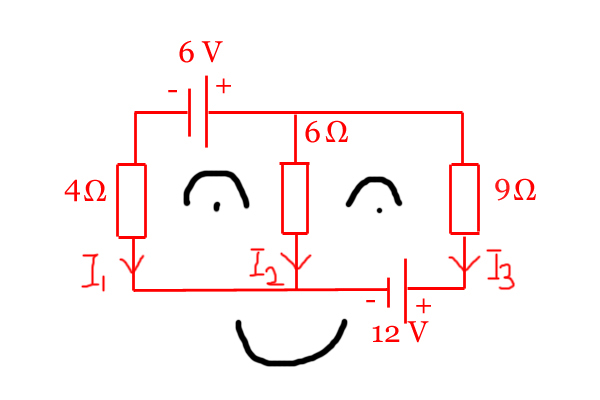
\includegraphics[scale = 0.4]{circuit.jpg}}
\caption{The circuit for Exercise \ref{ex:circuitsys}}
\label{fig:circuitsys}
\end{figure}\\
You will obtain two equations by considering any two loops with Kirchhoff’s Second Law, and one from Kirchhoff's First Law. So, there are three equations, for the three unknown currents.
\end{Exercise}
\begin{Answer}
The first two equations below come from the left inner loop and right inner loop, but one of them can be replaced by the outer loop as well.
\begin{align*}
-4I_1 + 6I_2 &= 6\\
-6I_2 + 9I_3 &= -12\\
I_1 + I_2 + I_3 &= 0
\end{align*}
and the solution is $I_1 = -\frac{3}{19}$, $I_2 = \frac{17}{19}$, $I_3 = -\frac{14}{19}$ (in Amperes).
\end{Answer}

\begin{Exercise}
\label{ex:shallowwater}
The \textit{shallow water equations} (see Figure \ref{fig:shallowwater}) describe the evolution of gravity wave under some approximations such as \textit{hydrostatic balance} and a sufficiently shallow fluid depth, and has the form of
\begin{align*}
\begin{dcases}
\frac{\partial \eta}{\partial t} + H(\frac{\partial u}{\partial x} + \frac{\partial v}{\partial y}) &= 0 \\
\frac{\partial u}{\partial t} &= -g\frac{\partial \eta}{\partial x} \\
\frac{\partial v}{\partial t} &= -g\frac{\partial \eta}{\partial y} 
\end{dcases}
\end{align*}
when the Coriolis effect is ignored. By assuming a travelling wave solution
\begin{align*}
u &= \tilde{U} \cos(kx + ly - \omega t) \\
v &= \tilde{V} \cos(kx + ly - \omega t) \\
\eta &= \tilde{\eta} \cos(kx + ly - \omega t)
\end{align*}
where $\tilde{U}$, $\tilde{V}$, $\tilde{\eta}$ are some constants to be determined, show that the equations become
\begin{align*}
\begin{dcases}
\omega \tilde{\eta} - kH \tilde{U} - lH \tilde{V} &= 0 \\
\omega \tilde{U} - kg \tilde{\eta} &= 0 \\
\omega \tilde{V} - lg \tilde{\eta} &= 0
\end{dcases}
\end{align*}
By requiring that $\tilde{U}$, $\tilde{V}$, $\tilde{\eta}$ have a non-trivial solution so that they are not all zeros, derive the dispersion relation of gravity wave, which is
\begin{align*}
\omega^2 &= gH(k^2 + l^2) \\
\omega &= c\kappa
\end{align*}
where $c = \sqrt{gH}$ is the wave speed, and $\kappa = \sqrt{k^2 + l^2}$ is the total wavenumber.
\end{Exercise}
\begin{figure}
\centering
\begin{tikzpicture}
    \draw [thick,color=black,domain=0:3*pi,samples=500] plot (\x, {5+0.5*sin(deg(4*\x))});
    \fill [blue!30] (3*pi,0) -- (0,0) -- plot[domain=0:3*pi,samples=500]  (\x, {5+0.5*sin(deg(4*\x))});
    \draw [thick,color=black] (0,0) -- (3*pi, 0);
    \fill [Brown!50!Orange] (0,0) rectangle (3*pi, -1) node[above left, black]{Bottom};
    \draw [<->] (3*pi+0.2, 0) -- (3*pi+0.2, 5) node[midway, xshift=8]{$H$};
    \draw [<->,red] (0.575*pi, 5.6) -- (0.575*pi, 5) node[midway, xshift=-8]{$\eta$};
    \draw [dashed, black] (0, 5) -- (3*pi, 5);
    \draw [thick, Green] (0.575*pi, 5) -- (0.575*pi, 0) node[midway, xshift=-8]{$u$};
    \draw [thick, Green, ->] (0.575*pi, 4) -- (0.575*pi+1, 4);
    \draw [thick, Green, ->] (0.575*pi, 3) -- (0.575*pi+1, 3);
    \draw [thick, Green, ->] (0.575*pi, 2) -- (0.575*pi+1, 2);
    \draw [thick, Green, ->] (0.575*pi, 1) -- (0.575*pi+1, 1);
    \node at (8.75, 2.5) {Fluid};
\end{tikzpicture}
\caption{The $x$-$z$ cross-section of shallow water system in Exercise \ref{ex:shallowwater}. $\eta$ is the height of free surface, $H$ is the mean depth of the fluid, and $u$ is the fluid velocity along $x$-axis.}
\label{fig:shallowwater}
\end{figure}
\begin{Answer}
Substituting the given wave solution forms into the equation, we have
\begin{align*}
\begin{split}
&\omega\tilde{\eta}\sin(kx+ly-\omega t) + H(-k\tilde{U}\sin(kx+ly-\omega t) \\
& -l\tilde{V}\sin(kx+ly-\omega t)) = 0 \\    
\end{split} \\
& \omega\tilde{U}\sin(kx+ly-\omega t) = gk\tilde{\eta}\sin(kx+ly-\omega t) \\
& \omega\tilde{V}\sin(kx+ly-\omega t) = gl\tilde{\eta}\sin(kx+ly-\omega t)
\end{align*}
Cancelling out all the sine factors, we arrive at the linear system displayed in the question
\begin{align*}
\begin{dcases}
\omega \tilde{\eta} - kH \tilde{U} - lH \tilde{V} &= 0 \\
\omega \tilde{U} - kg \tilde{\eta} &= 0 \\
\omega \tilde{V} - lg \tilde{\eta} &= 0
\end{dcases}
\end{align*}
For $\tilde{U}$, $\tilde{V}$, $\tilde{\eta}$ to have a non-trivial solution other than all zeros, we require the determinant of the corresponding coefficient matrix to be zero according to Theorem \ref{thm:sqlinsysunique}, which leads to
\begin{align*}
\begin{vmatrix}
\omega & -kH & -lH \\
-kg & \omega & 0 \\
-lg & 0 & \omega
\end{vmatrix} &= 0 \\
\omega^3 - gHk^2\omega - gHl^2\omega &= 0 \\
\omega^2 - gH(k^2 + l^2) &= 0 
\end{align*}
as the dispersion relation of gravity wave.
\end{Answer}

\begin{Exercise}
Solve for the condensation height and temperature $z_{cd}$ and $T_{cd}$ in Exercise \ref{ex:lapse}.
\end{Exercise}
\begin{Answer}
$T_{cd} \approx \SI{15.9}{\celsius}$, $z_{cd} \approx \SI{0.97}{\km}$.
\end{Answer}

\begin{Exercise}
Solve the \textit{Chickens and Rabbits in the Same Cage} problem in Exercise \ref{ex:animals}. If we now introduce a new type of mystical creature who has one head and three legs, and throw them in another cage along with some chickens and rabbits, find all possible numbers of the three species if the cage now has $48$ heads and $122$ legs.
\end{Exercise}
\begin{Answer}
$x = 23$, $y = 12$. For the extra part, the new system of equations become (denote the number of third species as $z$)
\begin{align*}
\begin{bmatrix}
1 & 1 & 1 \\
2 & 4 & 3
\end{bmatrix}
\begin{bmatrix}
x \\
y \\
z
\end{bmatrix}
=
\begin{bmatrix}
48 \\
122
\end{bmatrix}
\end{align*}
By Gaussian Elimination, we have
\begin{align*}
\left[
\begin{array}{@{}ccc|c@{}}
1 & 1 & 1 & 48 \\
2 & 4 & 3 & 122
\end{array}
\right]
&\to
\left[
\begin{array}{@{}ccc|c@{}}
1 & 1 & 1 & 48 \\
0 & 2 & 1 & 26
\end{array}
\right] & R_2 - 2R_1 \to R_2 \\
&\to
\left[
\begin{array}{@{}ccc|c@{}}
1 & 1 & 1 & 48 \\
0 & 1 & \frac{1}{2} & 13
\end{array}
\right] & \frac{1}{2}R_2 \to R_2 \\
&\to
\left[
\begin{array}{@{}ccc|c@{}}
1 & 0 & \frac{1}{2} & 35 \\
0 & 1 & \frac{1}{2} & 13
\end{array}
\right] & R_1 - R_2 \to R_1
\end{align*}
Let $z = t$ as the free variable, then we have $y = 13 - \frac{1}{2}t$ and $x = 35-\frac{1}{2}t$, and hence
\begin{align*}
\begin{bmatrix}
x \\
y \\
z
\end{bmatrix}
=
\begin{bmatrix}
35-\frac{1}{2}t \\
13-\frac{1}{2}t \\
t
\end{bmatrix}
=
\begin{bmatrix}
35 \\
13 \\
0
\end{bmatrix}
+
t
\begin{bmatrix}
-\frac{1}{2} \\
-\frac{1}{2} \\
1
\end{bmatrix}
\end{align*}
Since the numbers of species must be a non-negative integer, the solution can be expressed in a more good-looking form of
\begin{align*}
\begin{bmatrix}
x \\
y \\
z
\end{bmatrix}
=
\begin{bmatrix}
35 \\
13 \\
0
\end{bmatrix}
+
s
\begin{bmatrix}
-1 \\
-1 \\
2
\end{bmatrix}
\end{align*}
where $s = \frac{t}{2}$, and the range of $s$ is $0, 1, \ldots, 13$ (when $s$ reaches $13$ there is no chicken remained).
\end{Answer}
\chapter{Introduction to Vectors}

After three chapters of discussion about matrices, it is time to talk about another closely related object type in linear algebra, namely, vectors. While \textit{vectors} and \textit{vector spaces} have strictly mathematical definitions which make them abstract, we will take a more physical point of view with the special case of (finite-dimensional) geometric vectors first.

\section{Definition and Operations of Geometric Vectors}

\subsection{Basic Structure of Vectors in the Real $n$-space $\mathbb{R}^n$}
A \index{Vector}\index{Vector!Geometric Vector}\keywordhl{(geometric) vector} is a physical quantity represented by an ordered tuple of \textit{components} (numbers), e.g. $(1, 8, 7, 4)$, $(1-\imath, 1+3\imath, 2)$. It has a \textit{magnitude (length)} and \textit{direction}, resembling an arrow. Some real-life examples are: two-dimensional flow velocity $(u, v)$, the relative position of an airplane to a ground radar $(x, y, z)$.
\begin{defn}[$n$-dimensional Geometric Vector]
\label{defn:geometvec}
A $n$-dimensional geometric vector consists of $n$ ordered numbers called \index{Components}\keywordhl{components} and are denoted by either an arrow or boldface, like $\vec{v}$ or $\textbf{v}$. It is usually written out in two forms, as a \textit{column vector} or an \textit{ordered $n$-tuple}:
\begin{align*}
\vec{v} &=
\begin{bmatrix}
v_1 \\
v_2 \\
v_3 \\
\vdots \\
v_n
\end{bmatrix}
=
(v_1, v_2, v_3, \ldots, v_n)^T
\end{align*}
\end{defn}
A $n$-dimensional vector can be treated as an $n \times 1$ (\index{Vector!Column Vector}\keywordhl{column vector}) as suggested above, or a $1 \times n$ matrix (\index{Vector!Row Vector}\keywordhl{row vector}) depending on the situation. The form of a column vector is taken more often than the row vector one and so the column form is assumed throughout the book if it is not further specified. That is why the superscript $^T$ is added for the $n$-tuple form to reflect that it is in fact a column vector despite written horizontally. \par
\begin{tikzpicture}
\draw[->] (-2.5,0)--(2.5,0) node[right]{$x$};
\draw[->] (0,-2.5)--(0,2.5) node[above]{$y$};
\draw[blue,->,line width=1.2] (0,0)--(2,1) node[anchor=south]{$\vec{v} = (2,1)^T$};
\draw[Gray,dashed] (2,1)--(2,0) node[below]{$x = 2$};
\draw[Gray,dashed] (2,1)--(0,1) node[left]{$y = 1$};
\node[below left]{$O$}; 
\end{tikzpicture}\\    
A 2D vector drawn in an x-y plane.\par
{\fbox{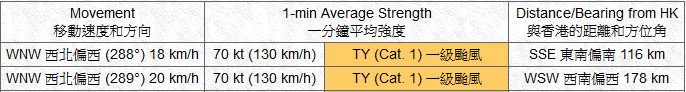
\includegraphics[scale = 0.5]{higos.jpg}}\\
Forecast for \textit{Typhoon Higos} (taken from \href{http://www.hkww.org/weather/tcarchive.html}{Hong Kong Weather Watch}). Its horizontal movement is a two-dimensional vector, even though the speed and direction are given instead of the velocities in $x$ and $y$-direction (they can be converted to each other).}

Implicit in the definition of $n$-dimensional vectors is the $n$-dimensional \textit{space} they are residing in. Assume the components of those vectors are all real, then the set of all such vectors constitutes the \index{Real $n$-space}\keywordhl{real $n$-space $\mathbb{R}^n$}.
\begin{defn}[The Real $n$-space $\mathbb{R}^n$]
\label{defn:real_nspace}
The real $n$-space $\mathbb{R}^n$ is defined as the set of all possible $n$-tuples $\vec{v} = (v_1, v_2, v_3, \ldots, v_n)^T$ as defined in Definition \ref{defn:geometvec}, where $v_i$ can take any \textit{real} value, for $i = 1,2,3,\ldots,n$. Such objects in $\mathbb{R}^n$ are known as $n$-dimensional \textit{real} vectors.
\end{defn}
While we have not clearly defined what a vector space is, we note that $\mathbb{R}^n$ fulfills the requirements of a vector space in a mathematical sense. A more detailed discussion of this aspect will be deferred to Chapter \ref{chap:vec_space}. Meanwhile, the complex counterpart will be explored in Chapter \ref{chap:complex}.\\
\\
An $n$-dimensional real geometric vector as described in Definition \ref{defn:geometvec} and \ref{defn:real_nspace} can be written as the sum of $n$ \index{Standard Unit Vector}\keywordhl{standard unit vectors} that have a magnitude of $1$ and are oriented in the positive direction along the $p$-th coordinates axes. They are denoted by $\hat{e}_p$, where $p$ can be from $1$ to $n$. The coordinate axes are perpendicular (or more generally, \textit{orthogonal}, introduced later in this chapter) to each other and this coordinate system is known as the \index{Cartesian Coordinate System}\keywordhl{Cartesian (coordinate) system}. Particularly, in the three-dimensional real space $\mathbb{R}^3$, $\hat{e}_1 = \hat{i} = (1,0,0)^T$, $\hat{e}_2 = \hat{j} = (0,1,0)^T$, $\hat{e}_3 = \hat{k} = (0,0,1)^T$ correspond to "an arrow" of length $1$ pointing in the positive direction of the $x$, $y$, $z$ axes respectively. 
\begin{defn}[Standard Unit Vector]
\label{defn:standardunitvec}
A standard unit vector $\hat{e}_p$ in the real $n$-space $\mathbb{R}^n$ (Definition \ref{defn:real_nspace}) has $n$ components, consisted of $1$ at the $p$-th entry and $0$ elsewhere. Mathematically, for $1\leq q \leq n$, $[\hat{e}_p]_q = 1$ when $q=p$ and $[\hat{e}_p]_q = 0$ when $q\neq p$.
\end{defn}
Below is an example of a geometric vector in the three-dimensional $xyz$ space ($\mathbb{R}^3$).
\begin{center}
\begin{tikzpicture}[x={(1.8cm, -0.4cm)}, y={(1.4cm, 1.2cm)}, z={(0cm, 2cm)}]
\draw [->] (0,0,0) -- (2,0,0) node [below right] {$x$};
\draw [->] (0,0,0) -- (0,2,0) node [above] {$y$};
\draw [->] (0,0,0) -- (0,0,2) node [left] {$z$};
\draw [->, thick, red, line width=1] (0,0,0) -- (1,0,0) node [below left] {$\hat{i} = (1,0,0)^T$};
\draw [->, thick, red, line width=1] (0,0,0) -- (0,1,0) node [above right, midway, sloped] {$\hat{j} = (0,1,0)^T$} ; 
\draw [->, thick, red, line width=1] (0,0,0) -- (0,0,1) node [left] {$\hat{k} = (0,0,1)^T$};
\draw [Gray, dashed] (1.8,0.4,0) -- (1.8,0,0) node[right, midway]{$y=0.4$}; 
\draw [Gray, dashed] (1.8,0.4,0) -- (0,0.4,0) node[above, midway, sloped]{$x=1.8$}; 
\draw [Gray, dashed] (1.8,0.4,0) -- (1.8,0.4,1.1) node[midway, right]{$z=1.1$};
\draw [->, blue, line width=1.2] (0,0,0) -- (1.8,0.4,1.1) node [right] {$\vec{v} = (1.8,0.4,1.1)^T$};
/\end{tikzpicture}
\begin{align*}
\vec{v} &= 
\begin{bmatrix}
1.8 \\
0.4 \\
1.1
\end{bmatrix}
= 1.8
\begin{bmatrix}
1 \\
0 \\
0
\end{bmatrix}
+ 0.4
\begin{bmatrix}
0 \\
1 \\
0
\end{bmatrix}
+ 1.1
\begin{bmatrix}
0 \\
0 \\
1
\end{bmatrix} 
= 1.8\hat{i} + 0.4\hat{j} + 1.1\hat{k} \\
&= (1.8,0.4,1.1)^T
\end{align*}
\end{center}
where we have written $\vec{v}$ in two forms, as an $n$-tuple and a sum of the three standard unit vectors $\hat{i}, \hat{j}, \hat{k}$.

\subsection{Fundamental Vector Operations}
\label{section:vectoraddmul}
\subsubsection{Addition and Subtraction}
Same as their matrix counterpart, addition and subtraction between vectors are component-wise, and hence only valid for vectors of the same dimension. For $\vec{w} = \vec{u} \pm \vec{v}$, we have $w_i = u_i \pm v_i$. If
\begin{align*}
&\vec{u} =
\begin{bmatrix}
1 \\
2
\end{bmatrix}
&
\vec{v} =
\begin{bmatrix}
2 \\
-1
\end{bmatrix}
\end{align*}
then
\begin{align*}
\vec{u} + \vec{v} =
\begin{bmatrix}
\textcolor{red}{1} \\
\textcolor{red}{2}
\end{bmatrix}
+
\begin{bmatrix}
\textcolor{blue}{2} \\
\textcolor{blue}{-1}
\end{bmatrix}
&= 
\begin{bmatrix}
\textcolor{Green}{3} \\
\textcolor{Green}{1}
\end{bmatrix}
\\
\vec{u} - \vec{v} =
\begin{bmatrix}
\textcolor{red}{1} \\
\textcolor{red}{2}
\end{bmatrix}
-
\begin{bmatrix}
\textcolor{blue}{2} \\
\textcolor{blue}{-1}
\end{bmatrix}
&= 
\begin{bmatrix}
\textcolor{Green}{-1} \\
\textcolor{Green}{3}
\end{bmatrix}
\end{align*}
\begin{center}
\begin{tikzpicture}[scale=0.8]
\draw[->] (-3.5,0)--(3.5,0) node[right]{$x$};
\draw[->] (0,-3.5)--(0,3.5) node[above]{$y$};
\draw[red,-stealth,line width=1] (0,0)--(1,2) node[anchor=south west]{$\vec{u} = (1,2)^T$};
\draw[blue,-stealth,line width=1] (1,2)--(3,1) node[anchor=south west]{$\vec{v} = (2,-1)^T$};
\draw[Green,-stealth,line width=1] (0,0)--(3,1) node[anchor=north west]{$\vec{u} + \vec{v} = (3,1)^T$};
\node[below left]{$O$}; 
\end{tikzpicture}\\
Addition: The tail of the blue vector is placed to the head of the red vector, and the resultant green vector is from the origin to the head of blue vector.
\end{center}
\begin{center}
\begin{tikzpicture}[scale=0.8]
\draw[->] (-3.5,0)--(3.5,0) node[right]{$x$};
\draw[->] (0,-3.5)--(0,3.5) node[above]{$y$};
\draw[red,-stealth,line width=1] (0,0)--(1,2) node[anchor=south west]{$\vec{u} = (1,2)^T$};
\draw[blue,-stealth,line width=1] (1,2)--(-1,3) node[anchor=south east]{$-\vec{v} = (-2,1)^T$};
\draw[Green,-stealth,line width=1] (0,0)--(-1,3) node[anchor=north east]{$\vec{u} - \vec{v} = (-1,3)^T$};
\node[below left]{$O$}; 
\end{tikzpicture}\\
Subtraction: Similar to addition but with the blue vector oriented in the opposite direction.
\end{center}

\subsubsection{Scalar Multiplication} 
Multiplying a scalar (be it a real or complex number) to a vector means that all components are multiplied by that scalar.
\begin{align*}
2
\begin{bmatrix}
2 \\
0 \\
1 \\
9
\end{bmatrix}
=
\begin{bmatrix}
4 \\
0 \\
2 \\
18
\end{bmatrix}
\end{align*}
Looking back at vector subtraction, it can be viewed as addition with a factor of $-1$ in the front.
\begin{align*}
\begin{bmatrix}
7 \\
5 \\
9
\end{bmatrix}
-
\begin{bmatrix}
3 \\
6 \\
9
\end{bmatrix}
=
\begin{bmatrix}
7 \\
5 \\
9
\end{bmatrix}
+ (-1)
\begin{bmatrix}
3 \\
6 \\
9
\end{bmatrix}
=
\begin{bmatrix}
7 \\
5 \\
9
\end{bmatrix}
+
\begin{bmatrix}
-3 \\
-6 \\
-9
\end{bmatrix}
=
\begin{bmatrix}
4 \\
-1 \\
0
\end{bmatrix}
\end{align*}

\subsubsection{Length and Unit Vector} \index{Length}\index{Magnitude}\keywordhl{Length (magnitude)}, or more formally \index{Euclidean Norm}\keywordhl{Euclidean norm}, of a vector $\vec{v}$ is based on a generalized version of \index{Pythagoras' Theorem}\keywordhl{Pythagoras' Theorem}, and is evaluated as the square root of the sum of squares of components.
\begin{defn}[Vector Length]
\label{defn:vectorlength}
Length, or magnitude of a $n$-dimensional \textit{real} vector $\vec{v}$, denoted by $\norm{\vec{v}}$, is given by
\begin{align*}
\norm{\vec{v}} &= \sqrt{v_1^2 + v_2^2 + v_3^2 + \cdots + v_n^2} \\
&= \sqrt{\sum_{k=1}^{n} v_k^2}
\end{align*}
\end{defn}
For instance, the length of a two-dimensional vector follows the usual Pythagoras' Theorem as below. \\
\begin{tikzpicture}
\draw[->] (-2.5,0)--(2.5,0) node[right]{$x$};
\draw[->] (0,-2.5)--(0,2.5) node[above]{$y$};
\draw[blue,-stealth,line width=1.2] (0,0)--(2,1) node[anchor=south west, align=left]{$\vec{v} = (2,1)^T$\\$\norm{\vec{v}} = \sqrt{x^2 + y^2} = \sqrt{2^2+1^2} = \sqrt{5}$};
\draw[Gray,dashed] (2,1)--(2,0) node[below]{$x = 2$};
\draw[Gray,dashed] (2,1)--(0,1) node[left]{$y = 1$};
\node[below left]{$O$}; 
\end{tikzpicture}\\
Here is another example which is three-dimensional.
\begin{center}
\begin{tikzpicture}[x={(1.8cm, -0.6cm)}, y={(1.6cm, 1.0cm)}, z={(0cm, 2cm)}]
\draw [->] (-1,0,0) -- (2,0,0) node [right] {$x$};
\draw [->] (0,-1,0) -- (0,2,0) node [above] {$y$};
\draw [->] (0,0,0) -- (0,0,2) node [left] {$z$};
\node[below] (0,0,0){$O$};
\draw [Gray, dashed] (1.6,-0.2,0) -- (1.6,0,0) node[below, pos=-0.5, sloped]{$y=-1$}; 
\draw [Gray, dashed] (1.6,-0.2,0) -- (0,-0.2,0) node[below, midway, sloped]{$x=8$}; 
\draw [Gray, dashed] (1.6,-0.2,0) -- (1.6,-0.2,0.8) node[midway, right]{$z=4$};
\draw [->, blue, line width=1.2] (0,0,0) -- (1.6,-0.2,0.8) node [right] {$\vec{w} = (8,-1,4)^T$};
\end{tikzpicture}
\begin{align*}
\vec{w} &= 
\begin{bmatrix}
8 \\
-1 \\
4
\end{bmatrix}
& \norm{\vec{w}}&=
\sqrt{8^2 + (-1)^2 + 4^2} = 9 
\end{align*}
\end{center}
We can create a \index{Vector!Unit Vector}\keywordhl{unit vector} that has a length of $1$ from any vector $\vec{v}$ and orients in the same direction as $\vec{v}$. It is simply created by dividing (normalizing) $\vec{v}$ by its distance $\norm{\vec{v}}$.
\begin{defn}[Unit Vector]
\label{defn:unitvec}
The unit vector corresponding to a non-zero vector $\vec{v}$ is denoted as $\hat{v}$ and is given by
\begin{align*}
\hat{v} &= \frac{1}{\norm{\vec{v}}}\vec{v}
\end{align*}
where the length $\norm{\vec{v}}$ is defined as in Definition \ref{defn:vectorlength}. 
\end{defn}
Note that despite vectors can carry physical units, unit vectors are all physically \textit{dimensionless} when formulated in this way. \\
\\
Short Exercise: Find the unit vector for $\vec{w} = (8, -1, 4)^T$ in the previous example, and verify that it has a length of $1$.\footnote{$\norm{\vec{w}} = 9$, $\hat{w} = \frac{\vec{w}}{\norm{\vec{w}}} = \frac{1}{9}(8,-1,4)^T = (\frac{8}{9}, -\frac{1}{9}, \frac{4}{9})^T$, $\norm{\hat{w}} = \sqrt{(\frac{8}{9})^2 + (-\frac{1}{9})^2 + (\frac{4}{9})^2} = 1$.}

\section{Special Vector Operations}
\label{section:vectorops}
Now we are going to introduce two special types of vector operations: \textit{dot product}, and \textit{cross product}. 

\subsection{Dot Product}
\label{section:dotprod}
\index{Dot Product}\keywordhl{(Real) Dot product} (or \index{Scalar Product}\keywordhl{scalar product}) is defined for two (real) vectors that have the same number of dimension. It is the sum of products of paired components between the two vectors. In other words, it can be regarded to be the matrix product between a row vector ($1 \times m$ matrix) and a column vector ($m \times 1$ matrix). 
\begin{defn}[Dot Product (Real)]
\label{defn:dotreal}
The dot product between two $n$-dimensional \textit{real} vectors $\vec{u}$ and $\vec{v}$ in $\mathbb{R}^n$ are denoted as either $\vec{u} \cdot \vec{v}$, or by matrix notation $\textbf{u}^T\textbf{v}$. They are defined as
\begin{align*}
\vec{u} \cdot \vec{v} = \textbf{u}^T\textbf{v} &= u_1v_1 + u_2v_2 + u_3v_3 + \cdots + u_nv_n \\
&= \sum_{k=1}^{n} u_kv_k
\end{align*}
which is a scalar quantity.
\end{defn}
Conversely, it can be said that entries of a matrix product are vector dot products between the corresponding rows and columns. It is emphasized that we are restricting ourselves to real entries since complex vectors introduce a bit of extra complications. Then, for two \textit{real} matrices expressed in the form of combined row/column vectors that are $\mathbb{R}^n$,
\begin{align*}
A &= \left[\begin{array}{@{}c@{}}
\text{---} \vec{u}^{(1)T} \text{---} \\
\hline
\text{---} \vec{u}^{(2)T} \text{---} \\
\hline
\vdots \\
\hline
\text{---} \vec{u}^{(p)T} \text{---}
\end{array}\right]
=  \left[\begin{array}{@{}c|c|c|c@{}}
| & | & & | \\
\vec{u}^{(1)} & \vec{u}^{(2)} & \cdots & \vec{u}^{(p)} \\
| & | & & |
\end{array}\right]^T
& B &= \left[\begin{array}{@{}c|c|c|c@{}}
| & | & & | \\
\vec{v}^{(1)} & \vec{v}^{(2)} & \cdots & \vec{v}^{(q)} \\
| & | & & |
\end{array}\right]\\
&= 
\begin{bmatrix}
\vec{u}^{(1)}_1  & \vec{u}^{(1)}_2 & \cdots & \vec{u}^{(1)}_n \\
\vec{u}^{(2)}_1  & \vec{u}^{(2)}_2 & \cdots & \vec{u}^{(2)}_n \\
\vdots & \vdots & & \vdots \\
\vec{u}^{(p)}_1  & \vec{u}^{(p)}_2 & \cdots & \vec{u}^{(p)}_n
\end{bmatrix} 
& &= 
\begin{bmatrix}
\vec{v}^{(1)}_1  & \vec{v}^{(2)}_1 & \cdots & \vec{v}^{(q)}_1 \\
\vec{v}^{(1)}_2  & \vec{v}^{(2)}_2 & & \vec{v}^{(q)}_2 \\
\vdots & & \ddots & \vdots \\
\vec{v}^{(1)}_n  & \vec{v}^{(2)}_n & \cdots & \vec{v}^{(q)}_n \\
\end{bmatrix} 
\end{align*}
(notice those transposes in the expression of $A$) their matrix product $AB$ can be written as
\begin{align*}
AB =
\begin{bmatrix}
\vec{u}^{(1)} \cdot \vec{v}^{(1)} & \vec{u}^{(1)} \cdot \vec{v}^{(2)} & \cdots & \vec{u}^{(1)} \cdot \vec{v}^{(q)} \\
\vec{u}^{(2)} \cdot \vec{v}^{(1)} & \vec{u}^{(2)} \cdot \vec{v}^{(2)} & \cdots & \vec{u}^{(2)} \cdot \vec{v}^{(q)} \\
\vdots & \vdots & & \vdots \\
\vec{u}^{(p)} \cdot \vec{v}^{(1)} & \vec{u}^{(p)} \cdot \vec{v}^{(2)} & \cdots & \vec{u}^{(p)} \cdot \vec{v}^{(q)} \\
\end{bmatrix}
\end{align*}
We can use dot product to express the length of a real vector.
\begin{proper}
\label{proper:lengthdot}
The length of a real vector, as defined in Definition \ref{defn:vectorlength}, can be written using its dot product between itself as
\begin{align*}
\norm{\vec{v}} &= \sqrt{\vec{v} \cdot \vec{v}} & &\text{or} &
\norm{\vec{v}}^2 &= \vec{v} \cdot \vec{v}
\end{align*}
\end{proper}
Notice that $\vec{v} \cdot \vec{v} = v_1^2 + v_2^2 + v_3^2 + \cdots + v_n^2 \geq 0$. This quantity is always strictly greater than zero ($\vec{v} \cdot \vec{v} > 0$) unless $\vec{v} = \textbf{0}$ is the zero vector (then $\vec{v} \cdot \vec{v} = 0$), which makes sense physically given that it represents length.

\begin{exmp}
\label{exmp:dotproduct5d}
If $\vec{u} = (1, 2, 3, 4, 5)^T$ and $\vec{v} = (-1, 0, 2, 1, -2)^T$, find the dot product $\vec{u} \cdot \vec{v} = \textbf{u}^T\textbf{v}$.
\end{exmp}
\begin{solution}
\begin{align*}
\vec{u} \cdot \vec{v} &= (1)(-1) + (2)(0) + (3)(2) + (4)(1) + (5)(-2) = -1
\end{align*}
Alternatively,
\begin{align*}
\textbf{u}^T\textbf{v} &=
\begin{bmatrix}
1 & 2 & 3 & 4 & 5
\end{bmatrix}
\begin{bmatrix}
-1 \\
0 \\
2 \\
1 \\
-2
\end{bmatrix}
= -1
\end{align*}
\end{solution}

Here are some properties of dot product.
\begin{proper}
\label{proper:dotproper}
For three $n$-dimensional real vectors $\vec{u}$, $\vec{v}$ and $\vec{w}$, the following properties hold.
\begin{align*}
\vec{u} \cdot \vec{v} &= \vec{v} \cdot \vec{u} &\text{Symmetry Property} \\
\vec{u} \cdot (\vec{v} \pm \vec{w}) &= \vec{u} \cdot \vec{v} \pm \vec{u} \cdot \vec{w} &\text{Distributive Property} \\
(\vec{u} \pm \vec{v}) \cdot \vec{w} &= \vec{u} \cdot \vec{w} \pm \vec{v} \cdot \vec{w} &\text{Distributive Property} \\
(a\vec{u}) \cdot (b\vec{v}) &= ab(\vec{u} \cdot \vec{v}) &\text{where $a$, $b$ are some constants}
\end{align*}
Additionally, if $A$ is an $n \times n$ square matrix, then
\begin{align*}
\vec{u} \cdot (A\vec{v}) &= \textbf{u}^T(A\textbf{v}) = (A^T\textbf{u})^T\textbf{v} = (A^T\vec{u}) \cdot \vec{v} \\
(A\vec{u}) \cdot \vec{v} &= (A\textbf{u})^T\textbf{v} = \textbf{u}^T(A^T\textbf{v}) = \vec{u} \cdot (A^T\vec{v})
\end{align*}
where we have used Definition \ref{defn:dotreal} and Properties \ref{proper:transp}.
\end{proper}
\begin{exmp}
For $\vec{u} = (1,3,1)^T$ and $\vec{v} = (2,-1,1)^T$, find $\norm{(\vec{u} + \vec{v})}^2 = (\vec{u} + \vec{v}) \cdot (\vec{u} + \vec{v})$.
\end{exmp}
\begin{solution}
By Properties \ref{proper:dotproper}, we can rewrite the expression as
\begin{align*}
(\vec{u} + \vec{v}) \cdot (\vec{u} + \vec{v}) &= \vec{u} \cdot (\vec{u} + \vec{v}) + \vec{v} \cdot (\vec{u} + \vec{v}) \\
&= \vec{u} \cdot \vec{u} + \vec{u} \cdot \vec{v} + \vec{v} \cdot \vec{u} + \vec{v} \cdot \vec{v} \\
&= \vec{u} \cdot \vec{u} + 2 \vec{u} \cdot \vec{v} + \vec{v} \cdot \vec{v}
\end{align*}
Subsequently,
\begin{align*}
&\quad \vec{u} \cdot \vec{u} + 2 \vec{u} \cdot \vec{v} + \vec{v} \cdot \vec{v} \\
&= (1,3,1)^T \cdot (1,3,1)^T + 2((1,3,1)^T \cdot (2,-1,1)^T) + (2,-1,1)^T \cdot (2,-1,1)^T \\
&= (1^2 + 3^2 + 1^2) + 2((1)(2)+(3)(-1)+(1)(1)) + (2^2 + (-1)^2 + 1^2) \\
&= 11 + 2(0) + 6 \\
&= 17
\end{align*}
Alternatively, one can calculate $\vec{w} = \vec{u} + \vec{v} = (1,3,1)^T + (2,-1,1)^T = (3,2,2)^T$ and find $\vec{w} \cdot \vec{w} = \norm{\vec{w}}^2$ instead. (which is easier and faster)
\end{solution}
\begin{exmp}
Given $\vec{u}$ and $\vec{v}$ as defined in the example above, if
\begin{align*}
A =
\begin{bmatrix}
1 & 2 & 1 \\
2 & 0 & 3 \\
1 & 1 & -1
\end{bmatrix}
\end{align*}
verify that $\vec{u} \cdot (A\vec{v}) = (A^T\vec{u}) \cdot \vec{v}$.
\end{exmp}
\begin{solution}
\begin{align*}
A\vec{v} &= 
\begin{bmatrix}
1 & 2 & 1 \\
2 & 0 & 3 \\
1 & 1 & -1
\end{bmatrix}
\begin{bmatrix}
2 \\
-1 \\
1
\end{bmatrix} \\
&=
\begin{bmatrix}
(1)(2) + (2)(-1) + (1)(1) \\
(2)(2) + (0)(-1) + (3)(1) \\
(1)(2) + (1)(-1) + (-1)(1) 
\end{bmatrix} \\
&=
\begin{bmatrix}
1 \\
7 \\
0
\end{bmatrix} \\
\vec{u} \cdot (A\vec{v}) &= (1,3,1)^T \cdot (1,7,0)^T \\
&= (1)(1) + (3)(7) + (1)(0) \\
&= 22
\end{align*}
On the other hand,
\begin{align*}
A^T\vec{u} &= 
\begin{bmatrix}
1 & 2 & 1 \\
2 & 0 & 1 \\
1 & 3 & -1
\end{bmatrix}
\begin{bmatrix}
1 \\
3 \\
1
\end{bmatrix} \\
&=
\begin{bmatrix}
(1)(1) + (2)(3) + (1)(1) \\
(2)(1) + (0)(3) + (1)(1) \\
(1)(1) + (3)(3) + (-1)(1) 
\end{bmatrix} \\
&=
\begin{bmatrix}
8 \\
3 \\
9
\end{bmatrix} \\
(A^T\vec{u}) \cdot \vec{v} &= (8,3,9)^T \cdot (2,-1,1)^T \\
&= (8)(2) + (3)(-1) + (9)(1) \\
&= 22
\end{align*}
\end{solution}

\subsubsection{Geometric Meaning of Dot Product}
The geometric meaning of dot product is embedded in the relation below.
\begin{proper}
\label{proper:dotgeo}
For two real vectors $\vec{u}$ and $\vec{v}$ that are of the same dimension, we have
\begin{align*}
\vec{u} \cdot \vec{v} = \norm{\vec{u}}\norm{\vec{v}}\cos\theta
\end{align*}
where $\theta$ is the angle between $\vec{u}$ and $\vec{v}$. Furthermore, if $\hat{u}$ and $\hat{v}$ are unit vectors (Definition \ref{defn:unitvec}) such that $\norm{\vec{u}} = \norm{\vec{v}} = 1$, it reduces to
\begin{align*}
\hat{u} \cdot \hat{v} = \cos\theta    
\end{align*}
\end{proper}
This means that the dot product between two vectors $\vec{u}$ and $\vec{v}$ is geometrically the signed product between $\vec{u}$ and the parallel component (projection) of $\vec{v}$ onto $\vec{u}$ (or vice versa), which is illustrated in the figure below. While an angle has a clear physical meaning only in a two/three-dimensional space, such relation generalizes the idea of an angle to higher dimensions.
\begin{center}
\begin{tikzpicture}[scale=1.3]
\coordinate (0) at (0,0);
\coordinate (vecu) at (4,1);
\coordinate (vecv) at (1,2);
\draw[->](0)--(vecu) node[right]{$\vec{u}$};
\draw[->](0)--(vecv) node[above]{$\vec{v}$};
\draw[dashed] (1,2)--(24/17, 6/17);
\draw[red] (24/17+0.2, 6/17+0.05)--(24/17+0.15, 6/17+0.25)--(24/17-0.05, 6/17+0.2);
\pic[draw, "$\theta$", angle eccentricity=1.5] {angle = vecu--0--vecv};
\draw[blue, very thick] (0,0)--(24/17, 6/17) node[below, shift={(0mm, -2mm)}]{$\norm{\vec{v}}\cos\theta$};
\end{tikzpicture}
\end{center}
\begin{exmp}
Find the angle between $\vec{u}$ and $\vec{v}$ in Example \ref{exmp:dotproduct5d}.
\end{exmp}
\begin{solution}
From Example \ref{exmp:dotproduct5d}, we have $\vec{u} \cdot \vec{v} = -1$, and
\begin{align*}
\norm{\vec{u}} &= \sqrt{1^2 + 2^2 + 3^2 + 4^2 + 5^2} = \sqrt{55} \\
\norm{\vec{v}} &= \sqrt{(-1)^2 + 0^2 + 2^2 + 1^2 + (-2)^2} = \sqrt{10} 
\end{align*}
By Properties \ref{proper:dotgeo}, we have
\begin{align*}
\cos\theta &= \frac{\vec{u} \cdot \vec{v}}{\norm{\vec{u}}\norm{\vec{v}}} \\
&= \frac{-1}{(\sqrt{55})(\sqrt{10})} \\
&\approx -0.0426 \\
\theta &\approx \SI{1.613}{\radian} = \SI{92.44}{\degree}
\end{align*}
\end{solution}
By Properties \ref{proper:dotgeo}, if the absolute value of the dot product $|\vec{u} \cdot \vec{v}|$ is equal to $\norm{\vec{u}}\norm{\vec{v}}$, where $\vec{u}$ and $\vec{v}$ are non-zero vectors, then it implies that $\cos\theta = \pm 1$, $\theta$ is either $0$ or $\pi$, and hence the two vectors are parallel. In constrast,
\begin{proper}
\label{proper:dotorth}
If the dot product between two real vectors $\vec{u}$ and $\vec{v}$ is zero ($\vec{u} \cdot \vec{v} = \vec{v} \cdot \vec{u} = 0$), then by Properties \ref{proper:dotgeo}, $\cos\theta = 0$ and the angle $\theta$ between $\vec{u}$ and $\vec{v}$ is $\frac{\pi}{2}$. In this case, $\vec{u}$ and $\vec{v}$ are said to be perpendicular, or \textit{orthogonal} to each other.
\end{proper}
From this, the concept of "\index{Orthogonal}\keywordhl{orthogonal}" becomes an extension of "perpendicular" in higher dimensions. It is easy to see that the standard unit vectors of $\mathbb{R}^n$ are orthogonal. Note that \textit{the zero vector is regarded to be orthogonal to any vector}, so even if $\vec{u}$ or $\vec{v}$ is a zero vector, this properties still hold. \par
Some may notice that as $-1 \leq \cos\theta \leq 1$, if $|\vec{u} \cdot \vec{v}| > \norm{\vec{u}}\norm{\vec{v}}$, then $\theta$ in Properties \ref{proper:dotgeo} will be ill-defined. However, the \index{Cauchy–Schwarz Inequality}\keywordhl{Cauchy–Schwarz Inequality} ensures this will not happen.
\begin{thm}[Cauchy–Schwarz Inequality]
\label{thm:CauchySch}
Given two \textit{real} $n$-dimensional vectors $\vec{u}$ and $\vec{v}$ ($\vec{u}, \vec{v} \in \mathbb{R}^n$), the following inequality holds.
\begin{align*}
|\vec{u} \cdot \vec{v}| &\leq \norm{\vec{u}}\norm{\vec{v}} \\
|u_1v_1+u_2v_2+\cdots+u_nv_n| &\leq \sqrt{u_1^2+u_2^2+\cdots+u_n^2}\sqrt{v_1^2+v_2^2+\cdots+v_n^2}
\end{align*}
\end{thm}
\begin{proof}
Consider $\vec{w} = \vec{u} + t\vec{v}$, where $t$ is any scalar, then $\norm{\vec{w}}^2 = \vec{w}\cdot\vec{w} \geq 0$ by Properties \ref{proper:lengthdot}. Also, $\vec{w}\cdot\vec{w}$ can be written as a quadratic polynomial in $t$:
\begin{align*}
\vec{w}\cdot\vec{w} = (\vec{u} + t\vec{v}) \cdot (\vec{u} + t\vec{v}) = \norm{\vec{u}}^2 + 2t(\vec{u} \cdot \vec{v}) + t^2\norm{\vec{v}}^2
\end{align*}
Since this quantity is always greater than or equal to zero, i.e.\ the quadratic polynomial has no root or a repeated root, it means that the discriminant must be negative or zero. So,
\begin{align*}
\Delta = b^2 - 4ac &\leq 0 \\
(2(\vec{u} \cdot \vec{v}))^2 - 4\norm{\vec{u}}^2\norm{\vec{v}}^2 &\leq 0 \\
(\vec{u} \cdot \vec{v})^2 - \norm{\vec{u}}^2\norm{\vec{v}}^2 &\leq 0 \\
(\vec{u} \cdot \vec{v})^2 &\leq \norm{\vec{u}}^2\norm{\vec{v}}^2 \\
|\vec{u} \cdot \vec{v}| &\leq \norm{\vec{u}}\norm{\vec{v}}
\end{align*}
\end{proof}
Short Exercise: Think about under what circumstances the Cauchy–Schwarz Inequality turns into an equality (i.e.\ $|\vec{u} \cdot \vec{v}| = \norm{\vec{u}}\norm{\vec{v}}$).\footnote{When $\vec{u}$ and $\vec{v}$ are parallel, i.e. $\vec{u} = k\vec{v}$ for some scalar $k$, or $\vec{v} = \textbf{0}$.}

\begin{exmp}
Prove the \index{Cosine Law}\keywordhl{Cosine Law} by considering the triangle below
\begin{center}
\begin{tikzpicture}
\coordinate (0) at (0,0);
\draw[red,-{Latex[length=5mm, width=2mm]}] (0)--(5,1) node[right](vecu){$\vec{u}$};
\draw[blue,-{Latex[length=5mm, width=2mm]}] (0)--(-1,3) node[above](vecv){$\vec{v}$};
\pic[draw, "$\theta$", angle eccentricity=1.5] {angle = vecu--0--vecv};
\draw[Green,-{Latex[length=5mm, width=2mm]}] (-1,3)--(5,1) node[midway, above, shift={(0mm, 3mm)}]{$\vec{u} - \vec{v}$};
\end{tikzpicture}
\end{center}
and expanding the dot product $\norm{(\vec{u}-\vec{v})}^2 = (\vec{u}-\vec{v}) \cdot (\vec{u}-\vec{v})$.    
\end{exmp}
\begin{solution}
Let denote the lengths $\norm{\vec{u}}$, $\norm{\vec{v}}$, $\norm{(\vec{u}-\vec{v})}$ be $a$, $b$, $c$, then
\begin{align*}
c^2 = \norm{(\vec{u}-\vec{v})}^2 &= (\vec{u}-\vec{v}) \cdot (\vec{u}-\vec{v}) & \text{(Properties \ref{proper:lengthdot})} \\
&= \vec{u} \cdot \vec{u} - \vec{u} \cdot \vec{v} - \vec{v} \cdot \vec{u} + \vec{v} \cdot \vec{v} & \text{(Properties \ref{proper:dotproper})} \\
&= \norm{\vec{u}}^2 - 2\vec{u} \cdot \vec{v} + \norm{\vec{v}}^2 & \text{(Properties \ref{proper:lengthdot} and \ref{proper:dotproper})} \\
&= \norm{\vec{u}}^2 - 2\norm{\vec{u}}\norm{\vec{v}}\cos\theta + \norm{\vec{v}}^2 & \text{(Properties \ref{proper:dotgeo})} \\
&= a^2 - 2ab\cos\theta + b^2
\end{align*}
\end{solution}

\subsection{Cross Product}
\label{section:crossprod}
Another important type of vector product is the \index{Cross Product}\keywordhl{cross product} (or sometimes just \index{Vector Product}\keywordhl{vector product}), which produces a three-dimensional real vector from two other three-dimensional real vectors. \textit{The output vector will be orthogonal to the two input vectors}, and the direction is determined by the \index{Right Hand Rule}\keywordhl{right hand rule}. Motivated by these requirements, we have the following basic definitions of cross product between the three standard unit vectors in $\mathbb{R}^3$.
\begin{defn}
\label{defn:crossijk}
The computation of cross products (denoted by $\times$) involving any two of the standard unit vectors $\hat{i}$, $\hat{j}$, $\hat{k}$ in $\mathbb{R}^3$ obeys the following rules.
\begin{enumerate}
\item $\hat{i} \times \hat{j} = \hat{k}$, $\hat{j} \times \hat{i} = -\hat{k}$,
\item $\hat{j} \times \hat{k} = \hat{i}$, $\hat{k} \times \hat{j} = -\hat{i}$,
\item $\hat{k} \times \hat{i} = \hat{j}$, $\hat{i} \times \hat{k} = -\hat{j}$, and
\item $\hat{i} \times \hat{i} = \hat{j} \times \hat{j} = \hat{k} \times \hat{k} = \textbf{0}$
\end{enumerate}
\end{defn}
\begin{minipage}{0.45\textwidth}
\begin{center}
% https://tex.stackexchange.com/questions/287284/drawing-a-diagram-of-a-three-cycle
\begin{tikzpicture}[->,scale=2]
   \node (i) at (90:1cm)  {\huge$\hat{i}$};
   \node (j) at (-30:1cm) {\huge$\hat{j}$};
   \node (k) at (210:1cm) {\huge$\hat{k}$};

   \draw (70:1cm)  arc (70:-10:1cm);
   \draw (-50:1cm) arc (-50:-130:1cm);
   \draw (190:1cm) arc (190:110:1cm);
\end{tikzpicture} \\
\end{center}
A cyclic diagram for memorizing Definition \ref{defn:crossijk}. A clockwise / anti-clockwise permutation produces a positive / negative unit vector of the third.
\end{minipage}
\hfill
\begin{minipage}{0.5\textwidth}
\begin{center}
% https://tikz.net/righthand_rule/
\begin{tikzpicture}[scale=0.8]
  \coordinate (O) at (1.0,0.7);
  \coordinate (WT) at ( 2.9,-1.1);
  \coordinate (T1) at ( 2.3, 0.7);
  \coordinate (T2) at ( 1.75, 2.3);
  \coordinate (T3) at ( 2.0, 3.1);
  \coordinate (T4) at (1.38, 3.15);
  \coordinate (T5) at ( 0.9, 2.3);
  \coordinate (T6) at ( 0.85, 1.2);
  \coordinate (T7) at ( 0.85, 0.2);
  \coordinate (I1) at (-1.1, 2.45);
  \coordinate (I2) at (-2.9, 3.45);
  \coordinate (I3) at (-3.3, 2.9);
  \coordinate (I4) at (-1.5, 1.8);
  \coordinate (I5) at (-0.9, 1.1);
  \coordinate (I6) at (-0.9, 0.3);
  \coordinate (M1) at (-2.1, 0.9);
  \coordinate (M2) at (-3.95,0.55);
  \coordinate (M3) at (-4.0,-0.15);
  \coordinate (M4) at (-2.3, 0.05);
  \coordinate (M5) at (-1.1, 0.20);
  \coordinate (R1) at (-1.9,-0.1);
  \coordinate (R2) at (-1.8,-0.7);
  \coordinate (R3) at (-0.3,-1.5);
  \coordinate (R4) at ( 0.1,-1.7);
  \coordinate (R5) at ( 0.1,-1.0);
  \coordinate (R6) at (-0.5,-0.7);
  \coordinate (R7) at (-1.2,-0.3);
  \coordinate (P1) at (-1.9,-1.3);
  \coordinate (P2) at (-0.8,-1.9);
  \coordinate (P3) at (-0.2,-2.1);
  \coordinate (P4) at (-0.05,-1.65);
  \coordinate (W1) at ( 0.4,-2.9);
  \coordinate (W2) at ( 1.6,-3.5);
  
  % HAND
  \fill[pink!25]
    (WT) -- (T6) -- (I5) -- (M5) -- (R2) -- (P2) -- (W2) to[out=25,in=-90] cycle;
  \draw[fill=pink!25]
    (WT) to[out=120,in=-60]
    (T1) to[out=120,in=-90]
    (T2) to[out=80,in=-110]
    (T3) to[out=80,in=50,looseness=1.5]
    (T4) to[out=-130,in=80]
    (T5) to[out=-100,in=70]
    (T6) to[out=-100,in=100]
    (T7)
    (T6) to[out=150,in=-30]
    (I1) to[out=150,in=-30]
    (I2) to[out=150,in=145,looseness=1.7]
    (I3) to[out=-30,in=150]
    (I4) to[out=-30,in=105]
    (I5) to[out=-75,in=90]
    (I6)
    (I5) to[out=-170,in=10]
    (M1) to[out=-170,in=10]
    (M2) to[out=-170,in=-175,looseness=1.8]
    (M3) to[out=5,in=-170]
    (M4) to[out=10,in=-170]
    (M5)
    (M5) to[out=-160,in=50]
    (R1) to[out=-130,in=140,looseness=1.2]
    (R2) to[out=-30,in=160]
    (R3) --
    (R4) to[out=-20,in=-20,looseness=1.5]
    (R5) --
    (R6) to[out=140,in=8,looseness=0.9]
    (R7)
    (R2) to[out=-160,in=155]
    (P1) to[out=-35,in=150]
    (P2) to[out=-30,in=160]
    (P3) to[out=-20,in=-30,looseness=1.5]
    (R4)
    (P2) to[out=-50,in=140]
    (W1) to[out=-40,in=160]
    (W2);
    
  \draw[->, blue, line width=1] (O) -- (128:3.2) coordinate(X) node[above=6,left=-6,scale=1.5] {$\vec{u}$};
  \draw[->, red, line width=1] (O) -- (-182:3.2) coordinate(Y) node[above=5,left=-6,scale=1.5] {$\vec{v}$};
  \draw[->, Purple, line width=2] (O) -- (62:3.2) node[above=-1,scale=1.5] {$\textcolor{blue}{\vec{u}} \textcolor{Purple}{\;\times\;} \textcolor{red}{\vec{v}}$};
  \draw pic[->, "$\theta$", draw=black, thick, angle radius=30, angle eccentricity=1.2] {angle = X--O--Y};
\end{tikzpicture}\\
Demonstration of the right hand rule.
\end{center}
\end{minipage}
\par
The properties of cross product are noted below. One major difference setting cross product apart from the dot product is its anti-symmetric property.
\begin{proper}
\label{proper:crossproper}
For two $\mathbb{R}^3$ vectors $\vec{u}$ and $\vec{v}$, we have
\begin{align*}
\vec{u} \times \vec{v} &= -\vec{v} \times \vec{u} &\text{Anti-symmetry Property} \\
\vec{u} \times (\vec{v} \pm \vec{w}) &= \vec{u} \times \vec{v} \pm \vec{u} \times \vec{w} &\text{Distributive Property} \\
(\vec{u} \pm \vec{v}) \times \vec{w} &= \vec{u} \times \vec{w} \pm \vec{v} \times \vec{w} &\text{Distributive Property} \\
(a\vec{u}) \times (b\vec{v}) &= ab(\vec{u} \times \vec{v}) &\text{where $a$, $b$ are some constants}
\end{align*}
\end{proper}
The calculation of cross product then follows from these rules, leading to the determinant shorthand below. 
\begin{proper}
\label{proper:crossdet}
For $\vec{u} = (u_1, u_2, u_3)^T, \vec{v} = (v_1, v_2, v_3)^T \in \mathbb{R}^3$, their cross product $\vec{u} \times \vec{v}$ can be written in the form of a determinant as
\begin{align*}
\vec{u} \times \vec{v} =
\begin{vmatrix}
\hat{i} & \hat{j} & \hat{k} \\
u_1 & u_2 & u_3 \\
v_1 & v_2 & v_3
\end{vmatrix}
\end{align*}
\end{proper}
\begin{proof}
Starting from Definition \ref{defn:crossijk} and Properties \ref{proper:crossproper}, we have
\begin{align*}
\vec{u} \times \vec{v} &= (u_1\hat{i} + u_2\hat{j} + u_3\hat{k}) \times (v_1\hat{i} + v_2\hat{j} + v_3\hat{k}) \\
&= u_1v_1(\hat{i}\times\hat{i}) + u_1v_2(\hat{i}\times\hat{j}) + u_1v_3(\hat{i}\times\hat{k}) \\
&\quad +u_2v_1(\hat{j}\times\hat{i}) + u_2v_2(\hat{j}\times\hat{j}) + u_2v_3(\hat{j}\times\hat{k}) \\
&\quad +u_3v_1(\hat{k}\times\hat{i}) + u_3v_2(\hat{k}\times\hat{j}) + u_3v_3(\hat{k}\times\hat{k}) & \text{(Properties \ref{proper:crossproper})}\\
&= u_1v_1(\textbf{0}) + u_1v_2(\hat{k}) - u_1v_3(\hat{j}) \\
&\quad -u_2v_1(\hat{k}) + u_2v_2(\textbf{0}) + u_2v_3(\hat{i}) \\
&\quad +u_3v_1(\hat{j}) - u_3v_2(\hat{i}) + u_3v_3(\textbf{0}) & \text{(Definition \ref{defn:crossijk})}\\
&= (u_2v_3 - u_3v_2)\hat{i} + (u_3v_1 - u_1v_3)\hat{j} + (u_1v_2 - u_2v_1)\hat{k} 
\end{align*}
Meanwhile, cofactor expansion (Properties \ref{proper:cofactorex}) along the first row of the given determinant form
\begin{align*}
\begin{vmatrix}
\hat{i} & \hat{j} & \hat{k} \\
u_1 & u_2 & u_3 \\
v_1 & v_2 & v_3
\end{vmatrix} 
&= 
\hat{i}
\begin{vmatrix}
u_2 & u_3 \\
v_2 & v_3
\end{vmatrix} 
- \hat{j}
\begin{vmatrix}
u_1 & u_3 \\
v_1 & v_3
\end{vmatrix} 
+ \hat{k}
\begin{vmatrix}
u_1 & u_2 \\
v_1 & v_2
\end{vmatrix} \\
&= (u_2v_3 - u_3v_2)\hat{i} + (u_3v_1 - u_1v_3)\hat{j} + (u_1v_2 - u_2v_1)\hat{k}
\end{align*}
yields the identical result.
\end{proof}

\begin{exmp}
Given two $\mathbb{R}^3$ vectors
\begin{align*}
&\vec{u} =
\begin{bmatrix}
1 \\
0 \\
2
\end{bmatrix}
&\vec{v} =
\begin{bmatrix}
3 \\
-1 \\
1
\end{bmatrix}
\end{align*}
Find $\vec{u} \times \vec{v}$.
\end{exmp}
\begin{solution}
\begin{align*}
\vec{u} \times \vec{v} &=
\begin{vmatrix}
\hat{i} & \hat{j} & \hat{k} \\
1 & 0 & 2 \\
3 & -1 & 1
\end{vmatrix} \\
&= 
\hat{i}
\begin{vmatrix}
0 & 2 \\
-1 & 1 
\end{vmatrix}
- \hat{j}
\begin{vmatrix}
1 & 2 \\
3 & 1 
\end{vmatrix}
+ \hat{k}
\begin{vmatrix}
1 & 0 \\
3 & -1 
\end{vmatrix}
& \begin{aligned}
\text{(Cofactor expansion} \\ 
\text{along the first row)}
\end{aligned}\\
&= 2\hat{i} + 5\hat{j} - \hat{k} = (2,5,-1)^T
\end{align*} 
\end{solution}
Short Exercise: Check if $\vec{u} \times \vec{v}$ is orthogonal to $\vec{u}$ and $\vec{v}$ by finding the corresponding dot products.\footnote{$\vec{u} \cdot (\vec{u} \times \vec{v}) = (1,0,2)^T\cdot(2,5,-1)^T = (1)(2) + (0)(5) + (2)(-1) = 0$, $\vec{v} \cdot (\vec{u} \times \vec{v}) = (3,-1,1)^T\cdot(2,5,-1)^T = (3)(2) + (-1)(5) + (1)(-1) = 0$. The zero dot product in both cases  shows they are orthogonal via Properties \ref{proper:dotorth}.}\\
Short Exercise: Following the short exercise above, show in general, $\vec{u} \cdot (\vec{u} \times \vec{v}) = \vec{v} \cdot (\vec{u} \times \vec{v}) = 0$.\footnote{From the derivation of Properties \ref{proper:crossdet}, $\vec{u} \times \vec{v} = (u_2v_3 - u_3v_2)\hat{i} + (u_3v_1 - u_1v_3)\hat{j} + (u_1v_2 - u_2v_1)\hat{k}$, and $\vec{u} \cdot (\vec{u} \times \vec{v}) = u_1(u_2v_3 - u_3v_2) + u_2(u_3v_1 - u_1v_3) + u_3(u_1v_2 - u_2v_1) = 0$ where all terms cancel out, and it is similar for $\vec{v}$.}


\subsubsection{Geometric Meaning of Cross Product} Similar to vector dot product, vector cross product has a geometric interpretation.
\begin{proper}
\label{proper:crossgeo}
Given two vectors $\vec{u}$ and $\vec{v}$ which are both of $\mathbb{R}^3$, the magnitude (length) of $\vec{u} \times \vec{v}$ is related to the angle between $\vec{u}$ and $\vec{v}$ as
\begin{align*}
\norm{\vec{u} \times \vec{v}} = \norm{\vec{u}}\norm{\vec{v}}\sin\theta
\end{align*}
\end{proper}
From this, we immediately know that if $\vec{u}$ and $\vec{v} = k\vec{u}$, where $k$ is some constant, are two parallel vectors, their cross product will be a zero vector as $\theta = 0$ (or $\pi$) and $\sin \theta = 0$. This is equivalent to the statement of $\vec{u} \times \vec{u} = \textbf{0}$\footnote{By Properties \ref{proper:crossdet},
\begin{align*}
\vec{u} \times \vec{u} = 
\begin{vmatrix}
\hat{i} & \hat{j} & \hat{k} \\
u_1 & u_2 & u_3 \\
u_1 & u_2 & u_3
\end{vmatrix} 
\end{align*} and the determinant vanishes by Properties \ref{proper:zerodet} due to the identical second/third row.} (notice that it is not $0$ but $\textbf{0}$ since it always outputs a vector!). (You can also arrive at this conclusion with Properties \ref{proper:crossproper}.\footnote{The anti-symmetric property requires $\vec{u}\times\vec{u} = -\vec{u}\times\vec{u}$ and hence $2(\vec{u}\times\vec{u}) = \textbf{0}$.})

\begin{exmp}
If $\vec{u} = (1,2,3)^T$, and $\vec{v} = (-1,1,2)^T$, find $(\vec{u} + 2\vec{v}) \times (\vec{u} - \vec{v}) $.
\end{exmp}
\begin{solution}
Observe that
\begin{align*}
(\vec{u} + 2\vec{v}) \times (\vec{u} - \vec{v}) &= \vec{u} \times (\vec{u} - \vec{v}) + 2\vec{v} \times (\vec{u} - \vec{v}) \\
&= \vec{u} \times \vec{u} - \vec{u} \times \vec{v} + 2\vec{v} \times \vec{u} - 2\vec{v} \times \vec{v} \\
&= \textbf{0} - \vec{u} \times \vec{v} - 2\vec{u} \times \vec{v} - 2(\textbf{0}) \\
&= -3\vec{u} \times \vec{v}
\end{align*}
where the fact that $\vec{u} \times \vec{u} = \textbf{0}$, $\vec{v} \times \vec{v} = \textbf{0}$ and Properties \ref{proper:crossproper} are used. Now, with Properties \ref{proper:crossdet}, we have
\begin{align*}
-3\vec{u} \times \vec{v} &=  
-3
\begin{vmatrix}
\hat{i} & \hat{j} & \hat{k} \\
1 & 2 & 3 \\
-1 & 1 & 2
\end{vmatrix} \\
&= -3\left(\hat{i}
\begin{vmatrix}
2 & 3 \\
1 & 2 
\end{vmatrix}
- \hat{j}
\begin{vmatrix}
1 & 3 \\
-1 & 2
\end{vmatrix}
+ \hat{k}
\begin{vmatrix}
1 & 2 \\
-1 & 1 
\end{vmatrix}\right) & \begin{aligned}
\text{(Cofactor expansion} \\ 
\text{along the first row)}
\end{aligned} \\
&= -3(\hat{i}-5\hat{j}+3\hat{k}) \\
&= -3\hat{i}+15\hat{j}-9\hat{k} = (-3,15,-9)^T
\end{align*}
The readers can try the alternative of computing $\vec{u}+2\vec{v}$ and $\vec{u} - \vec{v}$ first and then their cross product.
\end{solution}

Finally, cancellation of dot product or cross product at both sides of an equation is generally not correct, and here is a table summarizing the inputs and outputs of dot/cross product for clarification.
\begin{center}
\begin{tabular}{|p{30mm}|p{55mm}|p{25mm}|}
\hline
 & Input & Output \\
\hline
Dot Product, or Scalar Product ($\cdot$) & Two real vectors of the same dimension ($\mathbb{R}^n$), the order does not matter (symmetric) & A scalar\\
\hline
Cross Product, or Vector Product ($\times$) & Two three-dimensional real vectors ($\mathbb{R}^3$), the order is important (anti-symmetric) & Another three-dimensional vector
\\
\hline
\end{tabular}
\end{center}

\section{Earth Science Applications}
\begin{exmp}
\label{exmp:Coriolis}
The \textit{Coriolis Effect} is a phenomenon describing the deflection of motion due to rotation of the Earth. It introduces an apparent force known as the \textit{Coriolis Force} which is given by $\overrightarrow{F_\text{cor}} = -2\vec{\Omega} \times \vec{v}$ where $\Omega = \norm{\vec{\Omega}} = \SI{7.292e-5}{\radian \per \s}$ represents the angular speed of Earth's rotation, and $\vec{\Omega}$ is oriented in the direction of the North Pole. Define the local frame of reference (see Figure \ref{fig:Coriolis}) with the $x$-direction being the zonal direction, $y$-direction being the meridional direction, and $z$-direction being the zenith direction (normal to the Earth's surface), then we have $\vec{v} = (u,v,w) = u\hat{i} + v\hat{j} + w\hat{k}$ as the flow velocity in this local Cartesian coordinate system with unit vectors $\hat{i}, \hat{j}, \hat{k}$ along the $x$, $y$, $z$ axes. It can be seen that $\vec{\Omega} = (\Omega \cos\varphi) \hat{j} + (\Omega \sin \varphi) \hat{k}$ where $\varphi$ is the latitude. Now by expanding $\overrightarrow{F_\text{cor}} = -2\vec{\Omega} \times \vec{v}$ show that the components of Coriolis Force along the local $x,y,z$ directions are
\begin{align*}
F_{\text{cor},x} &= 2\Omega (v\sin\varphi - w\cos\varphi) \\
F_{\text{cor},y} &= -2\Omega u \sin\varphi \\
F_{\text{cor},z} &= 2\Omega u \cos\varphi
\end{align*}
The \textit{Coriolis Parameter} $f$ is usually used to denote the factor $2\Omega\sin\varphi$.
\end{exmp}
\begin{figure}[h!]
\centering
\begin{tikzpicture}
\coordinate (0) at (0,0);
\draw[black, bottom color=blue!40, top color=green!40, shading angle=-23.5] (0,0) circle (2);
\node[Mahogany] at (0,2.3) {Earth};
\draw[dashed,->] (66.5:-3) -- (66.5:3) node[above]{$\vec{\Omega}$};
\draw[dashed] (0) -- (-23.5:2) node(vecE){};
\path (0) -- (-23.5:2) node[midway, sloped, below]{Equator};
\draw[dashed] (0) -- (10:2) node(vecL){};
\draw pic["$\varphi$", draw=black, thick, angle eccentricity=1.5] {angle = vecE--0--vecL};
\draw[red, ->] (10:2) --++ (10:1.5) node[right]{$\hat{k}$};
\draw[red, ->] (10:2) --++ (100:1.5) node[above]{$\hat{j}$};
\draw[red, fill=gray!20] (10:2) circle (0.25) node[below right, yshift=-6]{$\hat{i}$};
\draw[red] (10:2) --++ (45:0.25);
\draw[red] (10:2) --++ (45:-0.25);
\draw[red] (10:2) --++ (-45:0.25);
\draw[red] (10:2) --++ (-45:-0.25);
\coordinate (P) at (5,-0.5);
\draw[red, ->] (P) --++ (10:1.5) node[right]{$\hat{k}$};
\draw[red, ->] (P) --++ (100:1.5) node[above](vecJ){$\hat{j}$};
\draw[dashed,->] (P) --++ (66.5:2) node[above](vecOM){};
\node at (8,1.7) {$\vec{\Omega} = (\Omega \cos \varphi)\hat{j} + (\Omega \sin \varphi)\hat{k}$};
\draw pic["$\varphi$", draw=black, thick, angle eccentricity=1.5] {angle = vecOM--P--vecJ};
\end{tikzpicture}
\caption{An illustration of the coordinate frame in Example \ref{exmp:Coriolis}.}
\label{fig:Coriolis}
\end{figure}
\begin{solution}
Using Properties \ref{proper:crossdet} to expand $\overrightarrow{F_\text{cor}}$ gives
\begin{align*}
-2\overrightarrow{\Omega} \times \vec{v} &= -2((\Omega \cos\varphi) \hat{j} + (\Omega \sin \varphi) \hat{k}) \times (u\hat{i} + v\hat{j} + w\hat{k}) \\
&= -2
\begin{vmatrix}
\hat{i} & \hat{j} & \hat{k} \\
0 & \Omega\cos\varphi & \Omega\sin\varphi \\
u & v & w 
\end{vmatrix} \\
&= -2[(w\Omega\cos\varphi - v\Omega\sin\varphi)\hat{i} + (u\Omega\sin\varphi)\hat{j} - (u\Omega\cos\varphi)\hat{k}] \\
&= [2\Omega(v\sin\varphi - w\cos\varphi)]\hat{i} + (-2\Omega u\sin\varphi)\hat{j} + (2\Omega u\cos\varphi)\hat{k}
\end{align*}
The $\hat{i}$, $\hat{j}$, $\hat{k}$ components correspond to $F_{\text{cor},x}$, $F_{\text{cor},y}$, $F_{\text{cor},z}$ respectively. Assume $w$ is negligible, then $F_{\text{cor},x} = fv$ and $F_{\text{cor},y} = -fu$.
\end{solution}

\section{Python Programming}
\label{section:ch4python}
We can use one-dimensional \verb|numpy| arrays as vectors. 
\begin{lstlisting}
import numpy as np

myVec1 = np.array([-1., 2., 4.])
myVec2 = np.array([2., 1., 3.])
\end{lstlisting}
Addition, subtraction, and scalar multiplication works just like for matrices.
\begin{lstlisting}
myVec3 = -myVec1 + 2*myVec2
print(myVec3)
\end{lstlisting}
gives the expected output of \verb|[5. 0. 2.]|. We can select a component of any vector by indexing. Again, remember that indices in \textit{Python} start from zero. \verb|print(myVec3[1])| then returns \verb|0.0|. The magnitude of a vector can be checked with \verb|np.linalg.norm|. For example,
\begin{lstlisting}
print(np.linalg.norm(myVec1))    
\end{lstlisting}
produces \verb|4.58257569495584| ($\sqrt{(-1)^2 + 2^2 + 4^2} = \sqrt{21}$). Dot product is computed via \verb|np.dot| as follows.
\begin{lstlisting}
myDot = np.dot(myVec1, myVec2)
print(myDot)
\end{lstlisting}
which outputs \verb|12.0| (as $(-1)(2) + (2)(1) + (4)(3) = 12$). Similarly, cross product is found by \verb|np.cross|.
\begin{lstlisting}
myCross = np.cross(myVec1, myVec2)
print(myCross)
\end{lstlisting}
then gives
\begin{lstlisting}
[ 2. 11. -5.]   
\end{lstlisting}
and we can check if the cross product is orthogonal to the two input vectors.
\begin{lstlisting}
# All lines below return zero.
print(np.dot(myVec1, myCross))
print(np.dot(myVec2, myCross))
print(np.dot(myVec3, myCross))
\end{lstlisting}
Dot product is defined for any two vectors with the same dimension, but cross product is only defined for three-dimensional vectors (or in some other sense two-dimensional), so
\begin{lstlisting}
myVec4 = np.array([1., 3., 2., 0.])
myVec5 = np.array([2., 1., 0., -1.])
print(np.dot(myVec4, myVec5))
\end{lstlisting}
yields a valid output of $5.0$, but
\begin{lstlisting}
print(np.cross(myVec4, myVec5))
\end{lstlisting}
raises the error of
\begin{lstlisting}
ValueError: incompatible dimensions for cross product
(dimension must be 2 or 3)    
\end{lstlisting}
Finally, we note that following \href{https://stackoverflow.com/questions/2827393/angles-between-two-n-dimensional-vectors-in-python}{this Stack Overflow post} (2827393), we can compute the unit vector of any given vector and angle between two vectors (based from the second observation in Properties \ref{proper:dotgeo}, $\theta = \cos^{-1}(\hat{u} \cdot \hat{v})$).
\begin{lstlisting}
def unit_vector(vector):
    """ Returns the unit vector of the vector.  """
    return vector / np.linalg.norm(vector)

def angle_between(v1, v2):
    """ Returns the angle in radians between vectors 'v1' and 'v2'. """
    v1_u = unit_vector(v1)
    v2_u = unit_vector(v2)
    return np.arccos(np.clip(np.dot(v1_u, v2_u), -1.0, 1.0))    
\end{lstlisting}
The \verb|np.clip| is to avoid numerical round-off error that causes the dot product of the two normalized input vectors to just fall outside (e.g. \verb|1.0000000000000002|) the valid range $[-1, 1]$ of $\cos^{-1}$. The naive way of (here the lists will be cast to one-dimensional arrays automatically during calculation.) 
\begin{lstlisting}
np.arccos(np.dot([1., 0, 0], [2., 0, 0]))
\end{lstlisting}
leads to the warning of
\begin{lstlisting}
RuntimeWarning: invalid value encountered in arccos  
nan
\end{lstlisting}
but
\begin{lstlisting}
angle_between([1., 0, 0], [2., 0, 0])
\end{lstlisting}
gives \verb|0.0| properly. Trying this on \verb|myVec4| and \verb|myVec5| with
\begin{lstlisting}
print(unit_vector(myVec4))
print(angle_between(myVec4, myVec5))
\end{lstlisting}
produces a unit vector of \verb|[0.267 0.802 0.535 0.   ]|, and an angle of \verb|0.993757| (in radians).

\section{Exercises}

\begin{Exercise}
For $\vec{u} = (1, 3, 3, 7)^T$ and $\vec{v} = (1, 2, 2, 5)^T$, find
\begin{enumerate}[label=(\alph*)]
\item $\vec{u} + \vec{v}$,
\item $\frac{3}{2}\vec{u} - \frac{1}{2}\vec{v}$,
\item $\vec{u} \cdot \vec{v}$,
\item $\vec{v} \cdot \vec{u}$,
\item $(\vec{u} - 2\vec{v}) \cdot (2\vec{u} + \vec{v})$.
\end{enumerate}
\end{Exercise}
\begin{Answer}
\begin{enumerate}[label=(\alph*)]
\item $(2, 5, 5, 12)^T$ 
\item $(1, \frac{7}{2}, \frac{7}{2}, 8)^T$
\item $(1)(1) + (3)(2) + (3)(2) + (7)(5) = 48$
\item $(1)(1) + (2)(3) + (2)(3) + (5)(7) = 48$
\item $\vec{u}-2\vec{v} = (-1, -1, -1, -3)^T, 2\vec{u} + \vec{v} = (3, 8, 8, 19)^T, (\vec{u} - 2\vec{v}) \cdot (2\vec{u} + \vec{v}) = (-1)(3) + (-1)(8) + (-1)(8) + (-3)(19) = -76$ 
\end{enumerate}
\end{Answer}

\begin{Exercise}
\label{ex:ch4prob_coplanar}
For $\vec{u} = (7, 4, 1)^T$, $\vec{v} = (8, 1, 1)^T$, and
\begin{align*}
A = 
\begin{bmatrix}
1 & 1 & 1\\
0 & 1 & 1\\
0 & 0 & 1
\end{bmatrix}
\end{align*}
Verify that
\begin{enumerate}[label=(\alph*)]
\item $\vec{u} \times \vec{v} = -\vec{v} \times \vec{u}$, 
\item $\vec{u} \cdot (\vec{Av}) = (A^T\vec{u}) \cdot \vec{v}$, 
\item Compute $(3\vec{u} - 4\vec{v}) \cdot (\vec{u} \times \vec{v})$, is the answer what you expect?
\end{enumerate}
\end{Exercise}
\begin{Answer}
\begin{enumerate}[label=(\alph*)]
\item 
\begin{align*}
\vec{u} \times \vec{v} &= 
\begin{vmatrix}
\hat{i} & \hat{j} & \hat{k}\\
7 & 4 & 1\\
8 & 1 & 1    
\end{vmatrix}
= 3\hat{i} + \hat{j} - 25\hat{k} = (3, 1, -25)^T \\
\vec{v} \times \vec{u} &=
\begin{vmatrix}
\hat{i} & \hat{j} & \hat{k}\\
8 & 1 & 1 \\  
7 & 4 & 1
\end{vmatrix}
= -3\hat{i} - \hat{j} + 25\hat{k} = (-3, -1, 25)^T
\end{align*} 
\item 
\begin{align*}
A\vec{v} &= 
\begin{bmatrix}
1 & 1 & 1\\
0 & 1 & 1\\
0 & 0 & 1
\end{bmatrix}
\begin{bmatrix}
8 \\
1 \\
1
\end{bmatrix}
=
\begin{bmatrix}
10 \\
2 \\
1
\end{bmatrix} \\
\vec{u} \cdot (\vec{Av}) 
&= (7, 4, 1)^T \cdot (10, 2, 1)^T \\
&= (7)(10) + (4)(2) + (1)(1) \\
&= 79 \\
A^T\vec{u} &= 
\begin{bmatrix}
1 & 0 & 0\\
1 & 1 & 0\\
1 & 1 & 1
\end{bmatrix}
\begin{bmatrix}
7 \\ 
4 \\
1
\end{bmatrix}
=
\begin{bmatrix}
7 \\
11 \\
12
\end{bmatrix} \\
(A^T\vec{u}) \cdot \vec{v}
&= (7, 11, 12)^T \cdot (8, 1, 1)^T \\
&= (7)(8) + (11)(1) + (12)(1) \\
&= 79 \\
\end{align*}
\item By (a), $\vec{u} \times \vec{v} = (3, 1, -25)^T$ and $(3\vec{u} - 4\vec{v}) = (-11,8,-1)^T$, then
\begin{align*}
(3\vec{u} - 4\vec{v}) \cdot (\vec{u} \times \vec{v}) &= (-11,8,-1)^T \cdot (3, 1, -25)^T \\
&= (-11)(3) + (8)(1) + (-1)(-25) = 0
\end{align*}
This makes sense as we have shown that $\vec{u} \cdot (\vec{u} \times \vec{v}) = \vec{v} \cdot (\vec{u} \times \vec{v}) = 0$, and therefore by distributive property $(\alpha\vec{u} + \beta\vec{v}) \cdot (\vec{u} \times \vec{v}) = 0$ for any $\alpha$ and $\beta$.
\end{enumerate}
\end{Answer}

\begin{Exercise}
For $\vec{u} = (1, -3, 9)^T$ and $\vec{v} = (1, -2, 4)^T$, find
\begin{enumerate}[label=(\alph*)]
\item Their unit vectors $\hat{u}$ and $\hat{v}$,
\item The angle between them, by calculating their dot product,
\item The cross product $\vec{u} \times \vec{v}$, and 
\item Show that the vector obtained from the cross product above is orthogonal (perpendicular) to $\vec{u}$ and $\vec{v}$, by calculating the corresponding dot products.
\end{enumerate}
\end{Exercise}
\begin{Answer}
\begin{enumerate}[label=(\alph*)]
\item 
\begin{align*}
\norm{\vec{u}} &= \sqrt{1^2 + (-3)^2 + 9^2} = \sqrt{91} \\
\hat{u} &= (\frac{1}{\sqrt{91}}, -\frac{3}{\sqrt{91}}, \frac{9}{\sqrt{91}})^T \\
\norm{\vec{v}} &= \sqrt{1^2 + (-2)^2 + 4^2} = \sqrt{21} \\
\hat{v} &= (\frac{1}{\sqrt{21}}, -\frac{2}{\sqrt{21}}, \frac{4}{\sqrt{21}})^T  
\end{align*}
\item 
\begin{align*}
\vec{u} \cdot \vec{v} = (1)(1) + (-3)(-2) + (9)(4) = 43 \\
\cos\theta = \frac{43}{\sqrt{21}\sqrt{91}} \approx 0.9836 \\
\theta \approx \SI{0.181}{\radian}    
\end{align*}
\item $\vec{u} \times \vec{v} = \begin{vmatrix}
\hat{i} & \hat{j} & \hat{k}\\
1 & -3 & 9\\
1 & -2 & 4
\end{vmatrix}
= 6\hat{i} + 5\hat{j} + \hat{k} = (6, 5, 1)^T$
\item $\vec{u} \cdot (\vec{u} \times \vec{v}) = (1, -3, 9)^T \cdot (6, 5, 1)^T = (1)(6) + (-3)(5) + (9)(1) = 0$, $\vec{v} \cdot (\vec{u} \times \vec{v}) = (1)(6) + (-2)(5) + (4)(1) = 0$
\end{enumerate}
\end{Answer}

\begin{Exercise}
The following table contains incomplete data about the movement of several typhoons at some moments. Complete the table by filling in the blanks. The first one has been done as an example.
\begin{center}
\footnotesize
\begin{tabular}{|c|c|c|c|c|}
\hline
Typhoon Name & Time & Speed & Direction & Vector Form\\
\hline
Nuri & 2008/08/22, 08:00 & \SI{13}{\km \per \hour} & \SI{315}{\degree} & $(-9.192, 9.192)$\\
\hline
Vicente & 2012/07/24, 02:00 & \SI{18}{\km \per \hour} & \SI{299}{\degree} & \\
\hline
Linfa & 2015/07/09, 23:00 & & & $(-13.595, -6.339)$\\
\hline
Mangkhut & 2018/09/16, 22:00 & & \SI{288}{\degree} & $(\quad, 7.725)$\\
\hline
\end{tabular}
\end{center}
\end{Exercise}
\begin{Answer}
\begin{center}
\footnotesize
\begin{tabular}{|c|c|c|c|c|}
\hline
Typhoon Name & Time & Speed & Direction & Vector Form\\
\hline
Nuri & 2008/08/22, 08:00 & \SI{13}{\km \per \hour} & \SI{315}{\degree} & $(-9.192, 9.192)$\\
\hline
Vicente & 2012/07/24, 02:00 & \SI{18}{\km \per \hour} & \SI{299}{\degree} & $\textcolor{red}{(-15.743, 8.727)}$\\
\hline
Linfa & 2015/07/09, 23:00 & \textcolor{red}{\SI{15}{\km \per \hour}} & \textcolor{red}{\SI{245}{\degree}} & $(-13.595, -6.339)$\\
\hline
Mangkhut & 2018/09/16, 22:00 & \textcolor{red}{\SI{25}{\km \per \hour}} & \SI{288}{\degree} & $(\textcolor{red}{-23.776}, 7.725)$\\
\hline
\end{tabular}
\end{center}    
\end{Answer}

\begin{Exercise}
\label{ex:triangular}
Prove the Triangular Inequality.
\begin{align*}
\norm{\vec{u} + \vec{v}} \leq \norm{\vec{u}} + \norm{\vec{v}}
\end{align*}
\end{Exercise}
\begin{Answer}
\begin{align*}
\norm{\vec{u} + \vec{v}}^2 &= (\vec{u} + \vec{v}) \cdot (\vec{u} + \vec{v}) \\
&= \norm{\vec{u}}^2 + 2(\vec{u}\cdot\vec{v}) + \norm{\vec{v}}^2 \\
&\leq \norm{\vec{u}}^2 + 2\norm{\vec{u}}\norm{\vec{v}} + \norm{\vec{v}}^2 \\
&= (\norm{\vec{u}} + \norm{\vec{v}})^2
\end{align*}
\end{Answer}

\begin{Exercise}
\phantomsection
\label{ex:parallellaw}
Prove the Parallelogram Law. (See Figure \ref{fig:parallellaw})
\begin{align*}
2\norm{\vec{u}}^2 + 2\norm{\vec{v}}^2 = \norm{\vec{u}+\vec{v}}^2 + \norm{\vec{u}-\vec{v}}^2
\end{align*}
\end{Exercise}
\begin{figure}
\centering
\begin{tikzpicture}
\draw[blue, ->] (0,0) -- (5,1) node[right]{$\vec{u}$};
\draw[red, ->] (0,0) -- (1,3) node[left]{$\vec{v}$};
\draw[Purple, ->] (1,3) -- (5,1) node[pos=0.75, sloped, above]{$\vec{u} - \vec{v}$};
\draw[Green, ->] (0,0) -- (6,4) node[pos=0.75, sloped, above]{$\vec{u} + \vec{v}$};
\draw[blue, dashed, ->] (1,3) -- (6,4);
\draw[red, dashed, ->] (5,1) -- (6,4);
\end{tikzpicture}
\caption{The parallelogram constructed by vectors for Exercise \ref{ex:parallellaw}.}
\label{fig:parallellaw}
\end{figure}
\begin{Answer}
\begin{align*}
\norm{\vec{u}+\vec{v}}^2 + \norm{\vec{u}-\vec{v}}^2 &= (\vec{u}+\vec{v}) \cdot (\vec{u}+\vec{v}) + (\vec{u}-\vec{v}) \cdot (\vec{u}-\vec{v}) \\
&= (\norm{\vec{u}}^2 + 2(\vec{u} \cdot \vec{v}) + \norm{\vec{v}}^2) + (\norm{\vec{u}}^2 - 2(\vec{u} \cdot \vec{v}) + \norm{\vec{v}}^2) \\
&= 2\norm{\vec{u}}^2 + 2\norm{\vec{v}}^2
\end{align*}
\end{Answer}

\begin{Exercise}
Show that Coriolis Force derived in Example \ref{exmp:Coriolis} does zero work and hence is consistent with the fact that it is an apparent force and never produces/consumes energy by itself.
\end{Exercise}
\begin{Answer}
In Example \ref{exmp:Coriolis}, we have
\begin{align*}
\overrightarrow{F_\text{cor}} &= (2\Omega(v\sin\varphi - w\cos\varphi))\hat{i} + (-2\Omega u\sin\varphi)\hat{j} + (2\Omega u\cos\varphi)\hat{k}    
\end{align*}
and hence the rate of work done is
\begin{align*}
&\quad \overrightarrow{F_\text{cor}} \cdot \vec{v} \\
&= [(2\Omega(v\sin\varphi - w\cos\varphi))\hat{i} + (-2\Omega u\sin\varphi)\hat{j} + (2\Omega u\cos\varphi)\hat{k}] \cdot (u\hat{i} + v\hat{j} + w\hat{k}) \\
&= (2\Omega(v\sin\varphi - w\cos\varphi))u + (-2\Omega u\sin\varphi)v + (2\Omega u\cos\varphi)w \\
&= 2\Omega uv\sin\varphi - 2\Omega uw\sin\varphi - 2\Omega uv\sin\varphi + 2\Omega uw\sin\varphi = 0
\end{align*}
Alternatively, note that $\overrightarrow{F_\text{cor}} = -2\overrightarrow{\Omega} \times \vec{v}$ and $({\Omega} \times \vec{v}) \cdot \vec{v} = 0$ always holds.
\end{Answer}
\chapter{More on Vector Geometry}

Vectors are a great tool to describe geometry. In this chapter we are going to exploit the knowledge learnt in the previous chapter to solve geometric problems.
\section{Lines and Planes}
Lines and planes are geometric objects of importance in 2D and 3D spaces and they are the first topics to be discussed. They can be expressed in terms of
(a) Equations, and (b) Vectors. We will start from talking lines which is easier.\\
\\
Since a line is a 1D object, the vector form of a line can be expressed mainly by a vector along its direction, times an arbitrary parameter which controls its length by extension or contraction, together with another arbitrary, fixed vector that represents its initial position.
\begin{center}
\begin{tikzpicture}
\draw[->] (0,0)--(4,0) node[right]{$x$};
\draw[->] (0,0)--(0,4) node[above]{$y$};
\draw[thick, ->] (0,0)--(0,1) node[left]{$\vec{r} = (0,1)^T$};
\draw[blue] (-0.4, 0.8)--(4.4, 3.2) node[left, shift={(0mm, 2mm)}]{$x - 2y = -2$};
\draw[Green, thick, ->] (0,0)--(2,2);
\draw[Green, thick, ->] (0,0)--(4,3);
\draw[Green, thick, ->] (0,0)--(1,1.5);
\draw[red, thick, ->] (0,1)--(2,2) node[left, shift={(0mm, 2mm)}]{$\vec{u} = (2,1)^T$};
\node[below left]{$O$}; 
\end{tikzpicture}\\
$\textcolor{Green}{\overrightarrow{OP}} = \vec{r} + \textcolor{blue}{t} \textcolor{red}{\vec{u}} = (0,1)^T + \textcolor{blue}{t} \textcolor{red}{(2,1)^T}$, the green arrow is controlled by $\textcolor{blue}{t}$ like a slider, the above graph shows the cases for $\textcolor{blue}{t} = 0.5, 1, 2$.
\end{center}
Short Exercise: Choose any value of $t$ and substitute it into the expression of $\overrightarrow{OP}$ to see if the $x$ and $y$-components satisfy the equation. Also, try to increase/decrease the value of $t$ to observe how the vector traces out a line.

\subsection{Translating Equation Form to Vector Form}
General form of equation of a line on x-y plane is $ax + by = h$, resembling a linear system of one equation with two unknowns. From Section \ref{subsection:SolLinSysGauss}, it can be observed that it has infinitely many solutions and possesses a free variable. Let $y = t$, then rearranging the equation we have $x = (h - bt)/a$ where $t$ is any scalar. Denote the origin as $O$ and any point on the line as $P$, then the vector from the origin to the line is
\begin{align*}
\overrightarrow{OP} =
\begin{bmatrix}
x \\
y
\end{bmatrix}
=
\begin{bmatrix}
\frac{h}{a} - \frac{b}{a}t\\
t
\end{bmatrix}
= 
\begin{bmatrix}
\frac{h}{a}\\
0
\end{bmatrix}
+ t
\begin{bmatrix}
-\frac{b}{a}\\
1
\end{bmatrix}
\end{align*}
This is the vector form of the line. The ideas behind can be borrowed from Example \ref{MulSol}, with $(h/a, 0)^T$ being the particular solution/initial position, and $(-b/a, 1)^T$ being the general solution/direction. For example, if we have $3x - 2y = 5$, then by the same method, we get
\begin{align*}
\begin{bmatrix}
x \\
y
\end{bmatrix}
=
\begin{bmatrix}
\frac{5}{3} + \frac{2}{3}t\\
t
\end{bmatrix}
= 
\begin{bmatrix}
\frac{5}{3}\\
0
\end{bmatrix}
+ t
\begin{bmatrix}
\frac{2}{3}\\
1
\end{bmatrix}    
\end{align*}
Bear in mind that the direction vector (general solution) can be scaled freely. In addition, any initial position vector (particular solution) can be chosen as long as it links to a point on the line, satisfying the equation. Hence there is no unique vector form for a line. For instance,
\begin{align*}
\begin{bmatrix}
1\\
3
\end{bmatrix}
+ t_1
\begin{bmatrix}
2 \\
4
\end{bmatrix}     
\end{align*}
is equivalent to
\begin{align*}
\begin{bmatrix}
-1\\
-1
\end{bmatrix}
+ t_2
\begin{bmatrix}
1 \\
2
\end{bmatrix}     
\end{align*}
for the line equation $2x - y = -1$.\\
Short Exercise: Verify the equivalence by choosing a value for $t_1$ and finding the corresponding $t_2$ so that the vector points to the same position.

\subsection{Recovering Equation Form from Vector Form} On the other hand, inferring line equation from the vector form is not straight-forward at first sight. Since the vector form of a line always contains an arbitrary parameter, which is absent in the equation form, the motivation is to remove the parameter through some manipulation.\\
\\
Remember that from Properties \ref{dotorth} the dot product between orthogonal (perpendicular) vectors returns zero. This means that by carrying out dot product with the vector orthogonal to the direction vector, namely the normal vector, on both sides of the vector form will eliminate the parameter and recover the line equation. For example, given that
\begin{align*}
\begin{bmatrix}
x\\
y
\end{bmatrix}
=
\begin{bmatrix}
1\\
3
\end{bmatrix}
+ t
\begin{bmatrix}
1 \\
4
\end{bmatrix} 
\end{align*}
We know that $(4, -1)^T$ is a vector orthogonal to the direction. So, by taking dot product with $(4, -1)^T$ on both sides, we have
\begin{align*}
\begin{bmatrix}
x\\
y
\end{bmatrix}
\cdot
\begin{bmatrix}
4\\
-1
\end{bmatrix}
&=
\begin{bmatrix}
1\\
3
\end{bmatrix}
\cdot
\begin{bmatrix}
4\\
-1
\end{bmatrix}
+ t
\begin{bmatrix}
1 \\
4
\end{bmatrix} 
\cdot
\begin{bmatrix}
4\\
-1
\end{bmatrix}\\
4x - y &= 1 + (0)t = 1
\end{align*}
Notice that the coefficients are the same as the components of the normal vector.\\
Short Exercise: Verify that $(a, b)$ is always orthogonal to $(b, -a)$, and vice versa.

\subsection{Generalizing to Higher Dimension}
Similar concepts can be applied on the equation and vector form for planes. General form of equation of a plane in 3D space is $ax + by + cz = h$, which is a linear system of one equation with three unknowns, implying two free variables and two direction vectors for such plane. By doing Gaussian Elimination, we obtain the vector form of the plane. \\
\\
Cross product of any two non-parallel vectors on the plane will give the third vector normal to the plane, then we can take the dot product with this new vector to convert the vector form back into a plane equation. Again, the coefficients of the plane equation match the components of the normal vector, differed at most by a factor.
\begin{center}
\begin{tikzpicture}[z={(-0.25,-0.5)}]
\filldraw[draw=red, fill=red!20]
(3,0,0) -- (0,3/2,0) -- (0,0,1) -- cycle;
\node[below right]{$O$}; 
\draw[thick,->] (0,0,0) -- (4,0,0) node[anchor=north east]{$x$};
\draw[thick,->] (0,0,0) -- (0,4,0) node[anchor=north west]{$y$};
\draw[thick,->] (0,0,0) -- (0,0,4) node[anchor=south east]{$z$};
\draw[very thick,->,blue] (0,3/2,0) -- (1,1,0) node[above right]{$(1, -1/2, 0)^T$};
\draw[very thick,->,blue] (0,3/2,0) -- (0,0,1) node[above left]{$(0, -3/2, 1)^T$};
\draw[very thick,->,red] (0,3/2,0) -- (3/2,9/2,9/2) node[above right]{Normal Vector $= (1/2, 1, 3/2)^T$};
\end{tikzpicture} \\
The plane represented by the equation $x + 2y + 3z = 3$. Notice that the normal vector can be found via computing $(0, -3/2, 1)^T \times (1, -1/2, 0)^T = (1/2, 1, 3/2)^T$. The normal vector is magnified for the purpose of illustration.
\end{center}

\begin{exmp}
For the equation $2x+3y+z = 4$, we can let $y=s$, $z=t$, then
\begin{align*}
\begin{bmatrix}
x \\
y \\
z
\end{bmatrix}
=
\begin{bmatrix}
(4-3s-t)/2 \\
s \\
t
\end{bmatrix}
=
\begin{bmatrix}
2 \\
0 \\
0
\end{bmatrix}
+ s
\begin{bmatrix}
-3/2 \\
1 \\
0
\end{bmatrix}
+ t
\begin{bmatrix}
-1/2 \\
0 \\
1
\end{bmatrix}
\end{align*}
where $-\infty < s < \infty$, $-\infty < t < \infty$ are some scalars. To recover the original equation, we can find the normal vector by doing cross product on the two vectors representing the general solutions.
\begin{align*}
\begin{bmatrix}
-3/2 \\
1 \\
0
\end{bmatrix}
\times
\begin{bmatrix}
-1/2 \\
0 \\
1
\end{bmatrix}
=
\begin{vmatrix}
\hat{i} & \hat{j} & \hat{k} \\
-3/2 & 1 & 0 \\
-1/2 & 0 & 1
\end{vmatrix}
= \hat{i} + \frac{3}{2}\hat{j} + \frac{1}{2}\hat{k}
\end{align*}
The next step is to take the dot product with the normal vector obtained above.
\begin{align*}
\begin{bmatrix}
x \\
y \\
z
\end{bmatrix}
&=
\begin{bmatrix}
2 \\
0 \\
0
\end{bmatrix}
+ s
\begin{bmatrix}
-3/2 \\
1 \\
0
\end{bmatrix}
+ t
\begin{bmatrix}
-1/2 \\
0 \\
1
\end{bmatrix} \\
\begin{bmatrix}
x \\
y \\
z
\end{bmatrix}
\cdot
\begin{bmatrix}
1 \\
3/2 \\
1/2
\end{bmatrix}
&=
\begin{bmatrix}
2 \\
0 \\
0
\end{bmatrix}
\cdot
\begin{bmatrix}
1 \\
3/2 \\
1/2
\end{bmatrix}
+ s
\begin{bmatrix}
-3/2 \\
1 \\
0
\end{bmatrix}
\cdot
\begin{bmatrix}
1 \\
3/2 \\
1/2
\end{bmatrix}
+ t
\begin{bmatrix}
-1/2 \\
0 \\
1
\end{bmatrix}
\cdot
\begin{bmatrix}
1 \\
3/2 \\
1/2
\end{bmatrix} \\
x + \frac{3}{2}y + \frac{1}{2}z &= 2 + (0)s + (0)t = 2
\end{align*}
\end{exmp}
The correspondence coefficients of a linear equation and its normal vector is not a coincidence. In fact, even for higher dimensional cases, where there is no simple geometric interpretation, we still have the following results.
\begin{thm}
\label{normalvec}
For an equation in the form of $a_1x_1 + a_2x_2 + a_3x_3 + \cdots + a_nx_n = h$, it has a normal vector of $(a_1, a_2, a_3, \cdots, a_n)^T$.
\end{thm}
The procedures carried in the last example can be similarly applied to higher dimensional circumstances.

\section{More on Geometric Applications of Dot Product}
\subsection{Projection}
The projection of a vector onto another vector can be derived from trigonometry and dot product. 
\begin{center}
\begin{tikzpicture}[scale=1.3]
\coordinate (0) at (0,0);
\draw[->](0)--(4,1) node[right](vecu){$\vec{u}$};
\draw[->](0)--(1,2) node[above](vecv){$\vec{v}$};
\draw[dotted] (1,2)--(24/17, 6/17);
\draw[red] (24/17+0.2, 6/17+0.05)--(24/17+0.15, 6/17+0.25)--(24/17-0.05, 6/17+0.2);
\pic[draw, ->, "$\theta$",angle eccentricity=1.5] {angle = vecu--0--vecv};
\draw[blue, very thick] (0,0)--(24/17, 6/17) node[below, shift={(0mm, -2mm)}]{$\norm{\vec{u}}\cos\theta$};
\end{tikzpicture}
\end{center}
By rearranging the relation stated in Properties \ref{dotgeo}, we have the magnitude of the projection of $\vec{u}$ onto $\vec{v}$ as
\begin{proper}
\label{proj}
Denote the projection of $\vec{u}$ onto $\vec{v}$ by $\text{proj}_v \vec{u}$, where $\vec{u}$ and $\vec{v}$ are both $m$-dimensional, then
\begin{align*}
\norm{\text{proj}_v \vec{u}} = \norm{\vec{u}} \cos\theta = \frac{\vec{u} \cdot \vec{v}}{\norm{\vec{v}}}    
\end{align*}
If we want to have the projection in the form of a vector, then we can utilize the unit vector along $\vec{v}$.
\begin{align*}
\text{proj}_v \vec{u} = \frac{\vec{u} \cdot \vec{v}}{\norm{\vec{v}}} \hat{v} = \frac{\vec{u} \cdot \vec{v}}{\norm{\vec{v}}^2} \vec{v} 
\end{align*}
where we have used Definition \ref{unitvec} for the second equation.
\end{proper}

\begin{exmp}
Find the projection of $\vec{u} = 2\hat{i} - 3\hat{j} + \hat{k}$ onto $\vec{v} = 4\hat{i} + \hat{j} - 3\hat{k}$ using Properties \ref{proj}.
\begin{align*}
\text{proj}_v \vec{u} &= \frac{\vec{u} \cdot \vec{v}}{\norm{\vec{v}}^2} \vec{v} \\
&= \frac{(2)(4)+(-3)(1)+(1)(-3)}{(4)^2+(1)^2+(-3)^2} (4\hat{i} + \hat{j} - 3\hat{k}) \\
&= \frac{1}{13} (4\hat{i} + \hat{j} - 3\hat{k}) = \frac{4}{13}\hat{i} + \frac{1}{13}\hat{j} - \frac{3}{13}\hat{k}
\end{align*}
The length of the projection is $\norm{\text{proj}_v \vec{u}} = \sqrt{(\frac{4}{13})^2 + (\frac{1}{13})^2 + (-\frac{3}{13})^2} = \frac{\sqrt{26}}{13}$.
\end{exmp}

\subsection{Distance} Distance of a point to a line/plane can be found by the projection of any vector connecting the point to the line/plane onto the normal vector of that line/plane, as shown in the figure below.
\begin{center}
\begin{tikzpicture}
\filldraw[draw=blue, fill=gray!20]
(0,0,0) -- (3,0,0) -- (3,0,3) -- (0,0,3) -- cycle;
\draw[thick,->,red] (1,0,1) -- (1,2.5,1) node[left]{Normal Vector $\vec{N}$};
\coordinate[label = {[Green]right:$P$}] (P) at (2,1.5,1.5);
\node at (P) [circle,fill,inner sep=1pt,Green]{};
\draw[thick,->,Green] (1,0,1) -- (2,1.5,1.5);
\draw[dotted, blue] (1,1.5,1) -- (2,1.5,1.5);
\draw[very thick, blue] (1,0,1) -- (1,1.5,1) node[left]{Distance = Projection of $\vec{P}$ onto $\vec{N}$};
\end{tikzpicture}
\end{center}

\begin{exmp}
Find the distance from the plane $x-2y+3z = 6$ to the point $(3,3,6)^T$.\\
\\
From the equation of the plane, and by Theorem \ref{normalvec}, it can be inferred that the normal vector of the plane is $\hat{i} - 2\hat{j} + 3\hat{k}$. We can select any point on the plane as we wish, let's say $(4,2,2)^T$, and the vector connecting it to the point $(3,3,6)^T$ is simply their difference $-\hat{i} + \hat{j} + 4\hat{k}$. Then the distance is found from the length of the projection of $-\hat{i} + \hat{j} + 4\hat{k}$ onto the normal vector of the plane $\hat{i} - 2\hat{j} + 3\hat{k}$. By Properties \ref{proj}, it is
\begin{align*}
\frac{(-\hat{i} + \hat{j} + 4\hat{k}) \cdot (\hat{i} - 2\hat{j} + 3\hat{k})}{\norm{\hat{i} - 2\hat{j} + 3\hat{k}}} = \frac{(-1)(1)+(1)(-2)+(4)(3)}{\sqrt{(1)^2 + (-2)^2 + (3)^2}} = \frac{9}{\sqrt{14}}
\end{align*}
\end{exmp}
Sometimes the calculation may lead to a negative value for the projection and we may want to take the absolute value.

\section{More on Geometric Applications of Cross Product}
\subsection{Area}
The area of the parallelogram formed by two vectors $\vec{u}$, $\vec{v}$ are simply the absolute value of their cross product.
\begin{center}
\begin{tikzpicture}
\coordinate (0) at (0,0);
\draw[thick, ->] (0)--(4,0) node[right](vecu){$\vec{u}$};
\draw[thick, ->] (0)--(1,3) node[above left](vecv){$\vec{v}$};
\draw[thick, ->, gray] (4,0)--(5,3);
\draw[thick, ->, gray] (1,3)--(5,3);
\draw[dotted, blue] (1,3)--(4,0);
\draw[dotted, gray] (1,3)--(1,0) node[midway, right]{$\norm{\vec{v}}\sin\theta$};
\draw[red] (1+0.15, 0)--(1+0.15, 0+0.15)--(1, 0+0.15);
\pic[draw, ->, "$\theta$",angle eccentricity=1.5] {angle = vecu--0--vecv};
\end{tikzpicture}
\end{center}
\begin{proper}
\label{parallelogram}
Directly by Properties \ref{crossgeo}, the area of the parallelogram formed by two vectors $\vec{u}$, $\vec{v}$ is
\begin{align*}
\norm{\vec{u} \times \vec{v}} = \norm{\vec{u}}\norm{\vec{v}}\sin\theta
\end{align*}
Similarly, the triangle built by $\vec{u}$, $\vec{v}$ is half of the quantity above, as
\begin{align*}
\frac{1}{2}\norm{\vec{u} \times \vec{v}} = \frac{1}{2}\norm{\vec{u}}\norm{\vec{v}}\sin\theta   
\end{align*}
\end{proper}

\begin{exmp}
Find the area of the parallelogram formed by $\vec{u} = (-1, -2, 4)^T$ and $\vec{v} = (3, 0, 1)^T$.\\
\\
The cross product between the given two vectors is
\begin{align*}
\vec{u} \times \vec{v} &=
\begin{vmatrix}
\hat{i} & \hat{j} & \hat{k} \\
-1 & -2 & 4 \\
3 & 0 & 1
\end{vmatrix} \\
&= -2\hat{i} + 13\hat{j} + 6\hat{k}
\end{align*}
Therefore, the required area is
\begin{align*}
\norm{\vec{u} \times \vec{v}} &= \sqrt{(-2)^2 + (13)^2 + (6)^2} \\
&= \sqrt{209}
\end{align*}
\end{exmp}

\subsection{Volume}
Meanwhile, volume of the parallelepiped formed by three vectors $\vec{u}$, $\vec{v}$, $\vec{w}$ is given by the absolute value of the so-called scalar triple product (since it outputs a number) as follows.
\begin{center}
\begin{tikzpicture}
\coordinate (0) at (0,0,0);
\draw[thick, ->] (0)--(4,0,0) node[right](vecu){$\vec{u}$};
\draw[thick, ->] (0)--(1,0,-2) node[below right](vecv){$\vec{v}$};
\draw[thick, ->] (0)--(1,3,-1) node[above left](vecw){$\vec{w}$};
\draw[thick, ->, gray] (4,0,0)--(5,0,-2);
\draw[thick, ->, gray] (1,0,-2)--(2,3,-3);
\draw[thick, ->, gray] (1,3,-1)--(5,3,-1);
\draw[thick, ->, gray] (4,0,0)--(5,3,-1);
\draw[thick, ->, gray] (1,0,-2)--(5,0,-2);
\draw[thick, ->, gray] (1,3,-1)--(2,3,-3);
\draw[thick, ->, gray] (5,0,-2)--(6,3,-3);
\draw[thick, ->, gray] (5,3,-1)--(6,3,-3);
\draw[thick, ->, gray] (2,3,-3)--(6,3,-3);
\draw[blue, dotted] (1,3,-1)--(1,0,-1) node[midway, right]{$\norm{\vec{w}}\cos\theta$};
\coordinate (P) at (1,0,-1);
\node at (P) [circle,fill,inner sep=1pt,blue]{};
\draw[thick, ->, red] (0,0,0) -- (0,3,0) node[above](vecn){$\vec{u}\times\vec{v}$};
\pic[draw, ->, "$\theta$",angle eccentricity=1.75] {angle = vecw--0--vecn};
\end{tikzpicture}
\end{center}
\begin{proper}
\label{parallelpiped}
The volume of the parallelepiped constructed by three vectors $\vec{u}$, $\vec{v}$, and $\vec{w}$ is
\begin{align*}
\norm{\vec{u} \times \vec{v}} \norm{\vec{w}} \cos\theta = |\vec{u} \cdot (\vec{v} \times \vec{w})| =
\text{abs}\left(
\begin{vmatrix}
u_1 & u_2 & u_3 \\
v_1 & v_2 & v_3 \\
w_1 & w_2 & w_3
\end{vmatrix}\right)
\end{align*}
where
\begin{align*}
\vec{u} \cdot (\vec{v} \times \vec{w}) =
\begin{vmatrix}
u_1 & u_2 & u_3 \\
v_1 & v_2 & v_3 \\
w_1 & w_2 & w_3
\end{vmatrix}    
\end{align*}
Also,
\begin{align*}
\vec{u} \cdot (\vec{v} \times \vec{w}) = (\vec{u} \times \vec{v}) \cdot \vec{w} 
\end{align*}
\end{proper}
If the volume of the parallelepiped evaluated from the scalar triple product is zero, it implies that the three constituent vectors are co-planar, lying on the same plane.
\begin{proper}
Given three vectors $\vec{u}$, $\vec{v}$, and $\vec{w}$, if $\vec{u} \cdot (\vec{v} \times \vec{w}) = 0$, $\vec{u}$, $\vec{v}$, and $\vec{w}$ are co-planar and all lie on the same plane.
\end{proper}
If $\vec{w} = \alpha \vec{u} + \beta \vec{v}$, where $\alpha$ and $\beta$ are some scalars, then $\vec{u}$, $\vec{v}$, $\vec{w}$ are co-planar, and $\vec{u} \cdot (\vec{v} \times \vec{w}) = 0$.

\begin{exmp}
Find the volume of the parallelepiped formed by $\vec{u} = (1,-2,2)^T$, $\vec{v}=(-1,-1,1)^T$ and $\vec{w}=(2,1,0)^T$.\\
\\
The triple scalar product is
\begin{align*}
\vec{u} \cdot (\vec{v} \times \vec{w}) &=
\begin{vmatrix}
1 & -2 & 2 \\
-1 & -1 & 1 \\
2 & 1 & 0
\end{vmatrix}
= -3
\end{align*}
So the volume is $\abs{-3} = 3$.
\end{exmp}

\paragraph{Remarks}
The solution of a linear system can be considered a point/line/plane, depending on the number of free variables (0/1/2). We may also like to call it a solution space. \\
\\
The method of assigning an arbitrary parameter to describe geometric objects is called parameterization. This can be applied for complex objects like cycloid, helix.\\
\\
Finally, while difficult to visualize geometrically, it is emphasized that the concept of free variables and parameterization can be extended to a linear equation of higher dimensions.

\section{Exercises}

\begin{Exercise}
Parameterize the following equation into vector form.
\begin{enumerate}[label=(\alph*)]
\item $6x + 8y = 9$,
\item $x + 9y + 9z = 7$,
\item $y = 3, -\infty < x < \infty$, and
\item $2x + z = 9, -\infty < y < \infty$.
\end{enumerate}
\end{Exercise}

\begin{Exercise}
Eliminate the parameters and find the direct equation.
\begin{enumerate}[label=(\alph*)]
\item \begin{align*}
\begin{bmatrix}
x\\
y
\end{bmatrix}
=
\begin{bmatrix}
2\\
9
\end{bmatrix}
+
t
\begin{bmatrix}
1\\
1
\end{bmatrix}
\end{align*}
\item \begin{align*}
\begin{bmatrix}
x\\
y\\
z
\end{bmatrix}
=
\begin{bmatrix}
6\\
3\\
2
\end{bmatrix}
+
s
\begin{bmatrix}
7\\
4\\
1
\end{bmatrix}
+
t
\begin{bmatrix}
8\\
0\\
5
\end{bmatrix}
\end{align*}
\end{enumerate}
where $-\infty < s,t < \infty$.
\end{Exercise}

\begin{Exercise}
Find the distance of the point $(3,2,9)^T$ to the plane $x + 2y + 5z = 10$, as well as the distance of the point $(3,2,9)^T$ to the line 
\begin{align*}
\begin{bmatrix}
x\\
y\\
z
\end{bmatrix}
=
t
\begin{bmatrix}
0\\
1\\
2
\end{bmatrix}
\end{align*}
where $-\infty < t < \infty$.
\end{Exercise}

\begin{Exercise}
Prove that the shortest distance between two lines, $\vec{u} = \vec{a} + s\hat{l}$ and $\vec{v} = \vec{b} + t\hat{m}$, where $-\infty < s,t < \infty$, $\vec{a}, \vec{b}$ are some arbitrary vectors and $\hat{l}, \hat{m}$ are some fixed, non-parellel unit vectors, is
\begin{align*}
\text{Dist}(u, v) = \frac{(\hat{a}-\hat{b}) \cdot (\hat{l} \times \hat{m})}{\norm{\hat{l} \times \hat{m}}}
\end{align*}
\end{Exercise}
What does it imply if $\vec{a} \cdot (\hat{l} \times \hat{m}) = \vec{b} \cdot (\hat{l} \times \hat{m})$?

\begin{Exercise}
Prove Sine Law with vector notation by considering the triangle below
\begin{center}
\begin{tikzpicture}
\draw[red,-{Latex[length=5mm, width=2mm]}] (0,0)--(2,3) node[midway, left]{$\vec{a}$};
\draw[blue,-{Latex[length=5mm, width=2mm]}] (2,3)--(4,1) node[midway, right]{$\vec{b}$};
\draw[Green,-{Latex[length=5mm, width=2mm]}] (4,1)--(0,0) node[midway, below]{$\vec{c}$};
\end{tikzpicture}
\end{center}
and equating three expressions of its area $\frac{1}{2}\norm{\vec{a}\times\vec{b}} = \frac{1}{2}\norm{\vec{b}\times\vec{c}} = \frac{1}{2}\norm{\vec{c}\times\vec{a}}$. Properties \ref{crossgeo} will be useful.
\end{Exercise}

\begin{Exercise}
By extending Properties \ref{parallelpiped}, derive a vector formula for the volume of a tetrahedron.
\begin{center}
\begin{tikzpicture}
\coordinate (0) at (0,0,0);
\draw[thick, ->] (0)--(4,0,0) node[right](vecu){$\vec{u}$};
\draw[thick, ->] (0)--(1,0,-2) node[above right](vecv){$\vec{v}$};
\draw[thick, ->] (0)--(1,3,-1) node[above left](vecw){$\vec{w}$};
\draw[thick, gray, dotted] (4,0,0)--(1,0,-2);
\draw[thick, gray, dotted] (1,3,-1)--(1,0,-2);
\draw[thick, gray, dotted] (1,3,-1)--(4,0,0);
\end{tikzpicture}
\end{center}
\end{Exercise}

\begin{Exercise}
For $\vec{u} = (1,2,3)^T$, $\vec{v} = (2,1,5)^T$, $\vec{w} = (1,4,0)^T$, find
\begin{enumerate}[label=(\alph*)]
\item Area of the parallelogram formed by $\vec{u}$ and $\vec{v}$,
\item Volume of the parallelepiped formed by $\vec{u}$, $\vec{v}$ and $\vec{w}$,
\item Redo the above for $\vec{w} = (1,5,4)^T$, what does the result tell you?
\end{enumerate}
\end{Exercise}

\begin{Exercise}
Find the geometric interpretation of solutions of the following systems of linear equations.
\begin{enumerate}[label=(\alph*)]
\item \begin{align*}
\begin{cases}
x + 2y + 2z &= 3\\
3x - y + 3z &= 2\\
x - 2y - z &= -1
\end{cases}
\end{align*}
\item
\begin{align*}
\begin{cases}
2x - y - z &= 3\\
x + y + 2z &= -1\\
x + 4y + 7z &= -6
\end{cases}
\end{align*}
\end{enumerate}
\end{Exercise}

\begin{Exercise}
\begin{enumerate}[label=(\alph*)]
\item Find a parameterization for $x^2 + 3y^2 = 4$, by using sine and cosine, and considering related trigonometric identity,
\item Find the direct relationship for $x = 4t^2 + 3t + 5$, $y = 2t + 1$,
\item Describe the geometric shape for the curve $x = \cos{t}$, $y = \sin{t}$, $z = \frac{t}{\pi}$.
\end{enumerate}
where $-\infty < t < \infty$.
\end{Exercise}
\chapter{Vector Spaces and Coordinate Bases}
\label{chap:6}

The previous chapters have provided a basic understanding of matrices and vectors respectively. What bridges these two quantities together is the concept of space and linear independence. They also lead to an essential geometric and physical idea about coordinate systems.

\section{Making of the Real $n$-Space $\mathbb{R}^n$}

\subsection{Spans by Linear Combination of Vectors}

\subsection{Linear Independence and Direct Sum}

\subsection{Forming Coordinate Bases for $\mathbb{R}^n$}

\subsection{Subspaces of $\mathbb{R}^n$}

\subsection*{Linear Combination and Linear Independence}
\label{6.1.1}

Linear combination of vectors $\vec{u_1}, \vec{u_2}, \vec{u_3}, \cdots$ is any expression in the form of $\vec{h} = c_1\vec{u_1} + c_2\vec{u_2} + c_3\vec{u_3} + \cdots$ where $c_j$ are some constants. 
\begin{defn}
A linear combination of vectors $\vec{u_1}, \vec{u_2}, \vec{u_3}, \cdots, \vec{u_n}$ has the form of
\begin{align*}
\sum_{j=1}^n c_j\vec{u_j} = c_1\vec{u_1} + c_2\vec{u_2} + c_3\vec{u_3} + \cdots + c_n\vec{u_n}
\end{align*}
where $c_j$ are some constants.
\end{defn}
An example would be, if there are two vectors $\vec{u} = (1,2)^T$ and $\vec{v} = (3,4)^T$, then $\vec{h} = (5,6)^T$ will be a linear combination of $\vec{u}$ and $\vec{v}$, since $\vec{h} = (5,6)^T = -(1,2)^T + 2(3,4)^T = -\vec{u} + 2\vec{v}$.\\
Short Exercise: If $\vec{h} = (1,4)^T$ instead, express $\vec{h}$ as a linear combination of $\vec{u}$ and $\vec{v}$.\\
\\
Attentive readers may realize that from the demonstration above, to decide if a vector $\vec{h}$ can be written as the linear combination of a set of other vectors $\vec{u_j}$ is equivalent to determining whether the linear system $A\vec{x} = \vec{h}$ has a solution, where $A$ equals to $[\vec{u_1}|\vec{u_2}|\vec{u_3}|\cdots]$ (writing out $\vec{u_j}$ in columns). The matrix product $A\vec{x}$ is a compact way to represent a linear combination.
\begin{proper}
\label{linearcombmatrix}
A linear combination $c_1\vec{u_1} + c_2\vec{u_2} + c_3\vec{u_3} + \cdots + c_n\vec{u_n}$ made by a set of vectors $\vec{u_1}, \vec{u_2}, \vec{u_3}, \cdots, \vec{u_n}$, can be expressed by the matrix product $A\vec{x}$, where
\begin{align*}
&A = [\vec{u_1}|\vec{u_2}|\vec{u_3}|\cdots|\vec{u_n}]
&\vec{x} =
\begin{bmatrix}
c_1 \\
c_2 \\
c_3 \\
\cdots \\
c_n
\end{bmatrix}
\end{align*}
with $c_j$ being some constants.
\end{proper}
Thus the short exercise at the beginning can be considered as a task to find out the solution for the system
\begin{align*}
\begin{bmatrix}
1 & 3 \\
2 & 4 \\
\end{bmatrix}
\begin{bmatrix}
c_1 \\
c_2
\end{bmatrix} =
\begin{bmatrix}
1 \\
4
\end{bmatrix}
\end{align*}

Now we are going to tackle the idea of linear independence, which has profound implications in linear algebra. Given a set of vectors that are all $m$-dimensional, if every one of them can not be expressed as the linear combination of other members, or in other words, they are not dependent on other vectors, then such set of vectors is said to be linearly independent. \\
\\
To check linear independence, one may try to show that for every vector it cannot be written as the linear combination of other vectors in the set. However, it is not plausible if the amount of vectors is large. Fortunately, we have a theorem which significantly simplfies our work.
\begin{thm}
\label{linearindep}
For a set of vectors $\vec{u_1}, \vec{u_2}, \vec{u_3}, \cdots, \vec{u_n}$, they are linearly independent if and only if, the linear system, $c_1\vec{u_1} + c_2\vec{u_2} + c_3\vec{u_3} + \cdots + c_n\vec{u_n} = \textbf{0}$ has $c_j = \textbf{0}$ as the unique solution. Using the matrix notation in Properties \ref{linearcombmatrix}, it means that the homogeneous system $A\vec{x} = \textbf{0}$ only has the trivial solution $c_j = \vec{x} = \textbf{0}$.
\end{thm}
\begin{exmp}
\label{exmplinearindep}
Determine if $\vec{u} = (1,2,1)^T$, $\vec{v} = (3,4,2)^T$, $\vec{w} = (6,8,1)^T$ are linearly independent.\\
\\
By Theorem \ref{linearindep}, this is equivalent to decide if $A\vec{x} = \textbf{0}$, where $A = [\vec{u}|\vec{v}|\vec{w}]$ has the trivial solution as the only solution. With the help of Theorem \ref{LinSysUnique}, we know that it is equivalent to check if $\text{det}(A)$ is zero or not. Since
\begin{align*}
|A| &=
\begin{vmatrix}
1 & 3 & 6\\
2 & 4 & 8 \\
1 & 2 & 1
\end{vmatrix} \\
&= 6 \neq 0
\end{align*}
We conclude that $A\vec{x} = \textbf{0}$ only has the trivial solution $\vec{x} = \textbf{0}$ and these three vectors are linearly independent.
\end{exmp}
Short Exercise: Repeat the above for $\vec{u} = (1,1,3)^T$, $\vec{v} = (1,3,2)^T$, $\vec{w} = (2,8,3)^T$.\\
\\
Including our earlier discussion in \autoref{chap:SolLinSys}, Theorem \ref{linearindep} gives some interesting results.
\begin{enumerate}
\item If the amount of vectors are greater than their dimension, i.e. 
$A = [\vec{u_1}|\vec{u_2}|\vec{u_3}|\cdots|\vec{u_n}]$ is an $m \times n$ matrix which has more columns ($n$) than rows ($m$), then $A\vec{x} = \textbf{0}$ must have at least one free variables and thus infinitely many solutions. Hence they must be linearly dependent.
\item Otherwise, we either find the solution of $A\vec{x} = \textbf{0}$ by Gaussian Elimination to see if it only has the trivial solution. Or if $A$ is a square matrix, then check if its determinant is non-zero (non-zero determinant implies only one solution, which in this case the trivial solution, just like Example \ref{exmplinearindep}). Gaussian Elimination still works for any square matrix, and in case of linear independence, $A$ will be reduced to an identity matrix.
\end{enumerate}
The above arguments also lead to an observation extending Theorem \ref{equiv2}.
\begin{thm}
\label{equiv3}
Invertibility of a square matrix $A$, Non-zero determinant $|A|$, Uniqueness of solution for the linear system $A\vec{x} = \vec{h}$, and linear independence for the column vectors $\vec{u_1}, \vec{u_2}, \vec{u_3}, \cdots, \vec{u_n}$ in $A = [\vec{u_1}|\vec{u_2}|\vec{u_3}|\cdots|\vec{u_n}]$, are all equivalent.
\end{thm}
This also completes our previous proof mentioned in Definition \ref{inverseidentity}.
\begin{thm}
If $AP = A$, and $A$ is a invertible square matrix, then $P$ must be $I$.
\paragraph{Proof}
The assumption implies that $A$ has linearly independent column vectors. As a result, they cannot be expressed by other vectors. Consider any one of the column vector, like $\vec{u_i}$, then the linear system
\begin{align*}
A\vec{x} &= ([\vec{u_1}|...|\vec{u_i}|...|\vec{u_n}])\vec{x} = x_1\vec{u_1} + \cdots + x_i\vec{u_i} + \cdots + x_n\vec{u_n} \\
&= \vec{u_i}
\end{align*}
will only have the solution
\begin{align*}
x_j &= 1 & \text{if $j = i$} \\
x_j &= 0 & \text{if $j \neq i$}
\end{align*}
This means that $\vec{x} = \hat{e_i}$. Now if we expand $P = [\vec{p_1}|\cdots|\vec{p_i}|\cdots|\vec{p_n}]$, then we can write $AP = A$ as
\begin{align*}
AP &= [A\vec{p_1}|\cdots|A\vec{p_i}|\cdots|A\vec{p_n}] \\
&= A = [\vec{u_1}|...|\vec{u_i}|...|\vec{u_n}]
\end{align*}
The readers are encouraged to verify the expression of $AP = [A\vec{p_1}|\cdots|A\vec{p_i}|\cdots|A\vec{p_n}]$ as a mental exercise, as from time to time we will partition such matrix product into columns. We have just found that for $A\vec{p_i} = \vec{u_i}$ to hold, $\vec{p_i}$ must be $\hat{e_i}$. This implies $P = [\hat{e_1}|...|\hat{e_i}|...|\hat{e_n}] = I$.
\end{thm}

\section{The Four Fundamental Subspaces Induced by Matrices}

\subsection{Row Space, Column Space, Null Space}

\subsection{Rank-Nullity Theorem}

As we have briefly mentioned in the last chapter, the solution of a linear system $A\vec{x} = \vec{h}$ can be viewed as a solution space. Complementing this idea is the related concept of column space, formed by the column vectors of the associated matrix $A$. We are not going to investigate the definition of a vector space in details, and will only talk about some basic aspects.
\begin{defn}
\label{columnspace}
Given a linear system $A\vec{x} = \vec{h}$, its column space includes all vectors that can be written as the linear combination of the column vectors in $A = [\vec{u_1}|\vec{u_2}|\vec{u_3}|\cdots|\vec{u_n}]$, or alternatively, all possible $A\vec{x}$ for every $\vec{x}$. Its solution space is the family of $\vec{x}$ that satisfies $A\vec{x} = \vec{h}$, inferred together by the particular solution and general solution.
\end{defn}
Solution space can be derived from the process of Gaussian Elimination, such as demonstrated in Example \ref{MulSol}. The dimension of solution space, sometimes referred to as its span, is the number of free variables. On the other hand, the span of the column space, is revealed by the amount of leading $1$ remained after Gaussian Elimination. Also, we have the following important theorem.
\begin{thm}
\label{span}
For a linear system $A\vec{x} = \vec{h}$, the span of the solution space is the number of columns in $A$ minus the span of the column space of $A$.
\end{thm}
\begin{exmp}
For the homogeneous system
\begin{align*}
\begin{bmatrix}
1 & 3 & 2\\
1 & 0 & 1\\
2 & -3 & 1
\end{bmatrix}
\begin{bmatrix}
x \\
y \\
z
\end{bmatrix}
=
\begin{bmatrix}
0\\
0\\
0
\end{bmatrix}
\end{align*}
Gaussian Elimination leads to
\begin{align*}
\left[\begin{array}{@{}ccc|c@{}}
1 & 0 & 1 & 0 \\
0 & 1 & 1/3 & 0 \\
0 & 0 & 0 & 0
\end{array}\right] 
\end{align*}
Two leading $1$ means that the column space is two-dimensional. Despite there are three column vectors to start with, one of them can be expressed with the other two column vectors. Also, the solution space includes all vectors in the form of $\vec{x} = t(-1, -1/3, 1)^T$, $-\infty < t < \infty$, which is one-dimensional. Theorem \ref{span} holds, as the number of columns minus the span of the column space is $3 - 2 = 1$ which is the span of the solution space.
\end{exmp}

Finally, we finish this section by linking linear independence (and thus invertibility), to the span of column space of a matrix $A$.
\begin{proper}
\label{invspan}
If $A$ is an invertible $n \times n$ square matrix, and thus has linearly independent column vectors, then Gaussian Elimination will turn $A$ into an identity matrix, which has $n$ leading $1$. By Theorem \ref{span}, the span of the column space will also be $n$.
\end{proper}

\section{More on Coordinate Bases}

\subsection*{Requirements for a Coordinate Basis, Standard Basis}
For a set of $m$-dimensional vectors to be the axes of a coordinate system in an $n$-dimensional vector space, it is intuitive that $m$ has to be equal to $n$. Apart from this, it is easy to see that the amount of vectors must also be greater than or equal to $n$, so that the column space may span the entire vector space. Another condition is that the vectors themselves are linearly independent, which needs the amount of vectors to be less than or equal to $n$. This ensures that any vector in the vector space can be uniquely determined by the coordinate basis, by the use of Theorem \ref{equiv3}. Taking all these requirements into account, we have the following conclusion.
\begin{proper}
In an $n$-dimensional vector space, any coordinate basis must be composed of $m$ linearly independent $m$-dimensional vectors, $m = n$. The matrix described in Properties \ref{invspan} satisfies the conditions.
\end{proper}
It is not difficult to see that the three vectors $\vec{u}$, $\vec{v}$ and $\vec{w}$ in Example \ref{exmplinearindep} are eligible to be a coordinate basis in a three-dimensional space.
A counter example would be $\vec{u} = (1,3)^T$, $\vec{v} = (-2,-6)^T$, where
\begin{align*}
\begin{vmatrix}
1 & -2 \\
3 & -6
\end{vmatrix}
= 0
\end{align*}
So they are linearly dependent. Any vector that is not a multiple of $(1,3)^T$ cannot be expressed by $\vec{u}$ and $\vec{v}$, and they are not a suitable coordinate basis for a two-dimensional space.
\begin{center}
\begin{tikzpicture}[scale = 0.3]
\draw[->] (-8,0)--(8,0) node[right]{$x$};
\draw[->] (0,-8)--(0,8) node[above]{$y$};
\draw[red,-stealth] (0,0)--(1,3) node[above right]{$\vec{u} = (1,3)^T$};
\draw[blue,-stealth] (0,0)--(-2,-6) node[below left]{$\vec{v} = (-2,-6)^T$};
\draw[Green,-stealth] (0,0)--(5,2) node[right]{$\vec{w} = (5,2)^T$};
\node[below left]{$O$}; 
\end{tikzpicture}\\
It is clear that $\vec{w}$ cannot be written as a linear combination of $\vec{u}$, $\vec{v}$ in this case.
\end{center}
In most of the time, the standard basis is used, i.e. 
$\hat{e_1} = (1, 0, 0, \cdots)^T$, $\hat{e_2} = (0, 1, 0, \cdots)^T$, $\hat{e_3} = (0, 0, 1, \cdots)^T$, etc. In three-dimensional Cartesian coordinates, it reduces to $\hat{i} = (1, 0, 0)^T, \hat{j} = (0, 1, 0)^T, \hat{k} = (0, 0, 1)^T$. It is used throughout previous parts. The standard basis is simple and natural.
More importantly, the standard basis vectors are of unit length and orthogonal to each other, making it an orthogonal basis. This means that the coordinate values for a vector relative to the basis is simply the projection of the vector onto the standard basis vectors, e.g. the projection of $\vec{v} = (3,4,5)^T$ onto the $x$-axis is simply $3$. It seems trivial, but actually it is not.

\subsection{Linear Coordinate Transformation}
\label{seccoordinatetrans}
Now we know what constitutes a coordinate basis, and there are many possible coordinate bases, we are tempted to transform the coordinate of a vector from one basis to another. We will first consider the transformation of any vector from the standard basis to an alternative basis, which can be done by finding the linear combination of the new basis vectors that reconstructs the targeted vector. Notice that physically the vector after transformation is still the same vector, but the coordinate values will be changed.\\
\\
It is equivalent to finding the solution for the system $A\vec{v_n} = \vec{v_0}$, where $\vec{v_n}$ and $\vec{v_0}$ are the coordinates in new basis and old basis respectively, $A$ is the transition matrix holding the vectors in the new basis in columns. We have $\vec{v_n} = A^{-1}\vec{v_0}$ if we multiply $A^{-1}$ at both sides. An example is supplied below to demonstrate the principle.
\begin{proper}
\label{coordinatetrans}
Coordinate transformation from a basis $B_u$ with $\vec{u_1}, \vec{u_2}, \cdots$, to the standard basis $B_s$, is done by
\begin{align*}
A\vec{v_n} &= \vec{v_0} \\
\vec{v_n} &= A^{-1}\vec{v_0}
\end{align*}
where $\vec{v_0}$ and $\vec{v_n}$ are the old and new coordinates respectively, $A = [\vec{u_1}|\vec{u_2}|\cdots]$.
\end{proper}
\begin{exmp}
Given a new basis $B_u$ that is consisted of $\vec{u_1} = (1,2)^T$ and $\vec{u_2} = (1,-1)^T$, transform a vector has the coordinate values $\vec{v_0} = (2,1)^T$ in the standard basis $B_s$ to $B_u$.\\
\\
Let $A = [\vec{u_1}|\vec{u_2}]$, then it can be seen that
\begin{align*}
&A =
\begin{bmatrix}
1 & 1 \\
2 & -1
\end{bmatrix}
&A^{-1} =
\begin{bmatrix}
1/3 & 1/3 \\
2/3 & -1/3
\end{bmatrix}
\end{align*}
Hence the new coordinates $\vec{v_n}$ is
\begin{align*}
\vec{v_n} = A^{-1}\vec{v_0} = 
\begin{bmatrix}
1/3 & 1/3 \\
2/3 & -1/3
\end{bmatrix}
\begin{bmatrix}
2 \\
1
\end{bmatrix}
=
\begin{bmatrix}
1\\
1
\end{bmatrix}
\end{align*}
\begin{center}
\begin{tikzpicture}[scale = 0.5]
\draw[->] (-5,0)--(5,0) node[right]{$x$};
\draw[->] (0,-5)--(0,5) node[above]{$y$};
\draw[red,-stealth] (0,0)--(2,4) node[above right]{$u_1$};
\draw[red,-stealth] (0,0)--(4,-4) node[below left]{$u_2$};
\draw[red, thick, dotted] (2,1)--(1,2) node[left]{$u_1 = 1$};
\draw[red, thick, dotted] (2,1)--(1,-1) node[right]{$u_2 = 1$};
\draw[blue,-stealth] (0,0)--(2,1) node[right]{$\vec{v_0} = (2,1)^T$, $\vec{v_n} = (1,1)^T$};
\node[below left]{$O$}; 
\end{tikzpicture}
\end{center}
Short Exercise: Recover $\vec{v_0}$ from $\vec{v_n}$.
\end{exmp}
To convert between two coordinate basis $B_u$ and $B_w$, we can first do the transformation from $B_u$ to the standard basis $B_s$, by $\vec{v_0} = A_u\vec{v_u}$, and then carry out another from $B_s$ to $B_w$, with $\vec{v_w} = A_w^{-1}\vec{v_0}$.

\begin{exmp}
A vector has the coordinates values $\vec{v_u} = (2,3)^T$ in the basis $B_u$ where $\vec{u_1} = (2,1)^T$, $\vec{u_2} = (-1,2)^T$. Convert its coordinates to the basis $B_w$ where $\vec{w_1} = (1,3)^T$, $\vec{w_2} = (-2,1)^T$.\\
\\
We first transform $\vec{v_u}$ to $\vec{v_0}$ using the standard basis.
\begin{align*}
\vec{v_0} &= A_u\vec{v_u} \\
&=
\begin{bmatrix}
2 & -1\\
1 & 2
\end{bmatrix}
\begin{bmatrix}
2 \\
3
\end{bmatrix}
=
\begin{bmatrix}
1 \\
8
\end{bmatrix}
\end{align*}
Subsequently, we do another transformation to the basis $B_w$.
\begin{align*}
\vec{v_w} &= A_w^{-1}\vec{v_0} \\
&=
\begin{bmatrix}
1 & -2\\
3 & 1
\end{bmatrix}^{-1}
\begin{bmatrix}
1 \\
8
\end{bmatrix} \\
&=
\begin{bmatrix}
1/7 & 2/7\\
-3/7 & 1/7
\end{bmatrix}
\begin{bmatrix}
1 \\
8
\end{bmatrix}
=
\begin{bmatrix}
17/7 \\
5/7
\end{bmatrix}
\end{align*}
\end{exmp}

\subsection{Gram-Schmidt Orthogonalization, QR Decomposition}

Sometimes the coordinate basis consists of vectors that are linearly independent but not orthogonal to each other, unlike the standard basis. A common way to create an orthogonal basis from the set is to apply the so-called Gram-Schmidt Orthogonalization.\\
\\
Basically, it is an iterative method. At each step it constructs a vector that are orthogonal to all the previously processed vectors by removing the parallel components projected onto them, extracting the orthogonal components.
\begin{center}
\begin{tikzpicture}[scale=1.3]
\coordinate (0) at (0,0);
\draw[->](0)--(4,1) node[right](vecu){$\vec{u_1}$, $\vec{v_1}$};
\draw[->](0)--(1,2) node[above](vecv){$\vec{u_2}$};
\draw[red, dotted, thick, ->] (24/17, 6/17)--(1,2) node[midway, right]{$\vec{v_2}$};
\draw[red] (24/17+0.2, 6/17+0.05)--(24/17+0.15, 6/17+0.25)--(24/17-0.05, 6/17+0.2);
\pic[draw, ->, "$\theta$",angle eccentricity=1.5] {angle = vecu--0--vecv};
\draw[blue, very thick] (0,0)--(24/17, 6/17) node[below, shift={(0mm, -2mm)}]{$\text{proj}_{v_1}\vec{u_2}$};
\end{tikzpicture}
\end{center}
For a set of vectors $\vec{u_1}, \vec{u_2}, \vec{u_3}, \cdots$ the orthogonal basis $\vec{v_1}, \vec{v_2}, \vec{v_3}, \cdots$ is generated by
\begin{defn}
Given a coordinate basis $\vec{u_1}, \vec{u_2}, \vec{u_3}, \cdots$, Gram-Schmidt Orthogonalization transforms them into $\vec{v_1}, \vec{v_2}, \vec{v_3}, \cdots$ according to the following formula.
\begin{align*}
\vec{v_1} &= \vec{u_1} \\
\vec{v_2} &= \vec{u_2} - \text{proj}_{v_1}\vec{u_2} = \vec{u_2} - \frac{\vec{v_1} \cdot \vec{u_2}}{\norm{\vec{v_1}}^2} \vec{v_1}\\
\vec{v_3} &= \vec{u_3} - \text{proj}_{v_1}\vec{u_3} - \text{proj}_{v_2}\vec{u_3} = \vec{u_3} - \frac{\vec{v_1} \cdot \vec{u_3}}{\norm{\vec{v_1}}^2} \vec{v_1} - \frac{\vec{v_2} \cdot \vec{u_3}}{\norm{\vec{v_2}}^2} \vec{v_2}\\
\vec{v_j} &= \vec{u_j} - \sum_{k=1}^{j-1}\text{proj}_{v_k}\vec{u_j}  = \vec{u_3} - \sum_{k=1}^{j-1}\frac{\vec{v_k} \cdot \vec{u_j}}{\norm{\vec{v_k}}^2} \vec{v_k}
\end{align*}
where the expression of projection, Properties \ref{proj}, is used.
\end{defn}
A variant of Gram-Schmidt Orthogonalization is to normalize every vector at each step immediately, such that $\norm{\hat{v_j}} = 1$ for all $j$, and the resulted basis is said to be orthonormal. The formula are then reduced to
\begin{defn}
\label{GSorth_norm}
Gram-Schmidt Orthogonalization with normalization at every iteration is given by
\begin{align*}
\hat{v_1} &= \frac{\vec{u_1}}{\norm{\vec{u_1}}} \\
\hat{v_2} &= \frac{\vec{u_2} - (\hat{v_1} \cdot \vec{u_2})\hat{v_1}}{\norm{\vec{u_2} - (\hat{v_1} \cdot \vec{u_2})\hat{v_1}}} \\
\hat{v_3} &= \frac{\vec{u_3} - (\hat{v_1} \cdot \vec{u_3})\hat{v_1} - (\hat{v_2} \cdot \vec{u_3})\hat{v_2}}{\norm{\vec{u_3} - (\hat{v_1} \cdot \vec{u_3})\hat{v_1} - (\hat{v_2} \cdot \vec{u_3})\hat{v_2}}} \\
\hat{v_j} &= \frac{\vec{u_j} - \sum_{k=1}^{j-1}(\hat{v_k} \cdot \vec{u_j})\hat{v_k}}{\norm{\vec{u_j} - \sum_{k=1}^{j-1}(\hat{v_k} \cdot \vec{u_j})\hat{v_k}}}
\end{align*}
\end{defn}
\begin{exmp}
\label{GSex}
Perform Gram-Schmidt Orthogonalization on the coordinate basis $\vec{u_1} = (1,3,5)^T$, $\vec{u_2} = (2,4,6)^T$, $\vec{u_3} = (8,3,2)^T$, using the formula in Definition \ref{GSorth_norm}.
\begin{align*}
\hat{v_1} &= \frac{1}{\sqrt{1^2+3^2+5^2}}
\begin{bmatrix}
1 \\
3 \\
5
\end{bmatrix} 
= 
\frac{1}{\sqrt{35}}
\begin{bmatrix}
1 \\
3 \\
5
\end{bmatrix} \\
\vec{u_2} - (\hat{v_1} \cdot \vec{u_2})\hat{v_1} &= 
\begin{bmatrix}
2 \\
4 \\
6
\end{bmatrix} 
-
((\frac{1}{\sqrt{35}})(2) + (\frac{3}{\sqrt{35}})(4) + (\frac{5}{\sqrt{35}})(6))
(\frac{1}{\sqrt{35}}
\begin{bmatrix}
1 \\
3 \\
5
\end{bmatrix}) \\
&= 
\begin{bmatrix}
2 \\
4 \\
6
\end{bmatrix} 
-
\textcolor{red}{\frac{44}{\sqrt{35}}}
(\frac{1}{\sqrt{35}}
\begin{bmatrix}
1 \\
3 \\
5
\end{bmatrix})
=
\frac{1}{35}
\begin{bmatrix}
26 \\
8 \\
-10
\end{bmatrix} \\
\hat{v_2} &= \frac{1}{\sqrt{26^2+8^2+(-10)^2}}
\begin{bmatrix}
26 \\
8 \\
-10
\end{bmatrix}
=
\frac{1}{2\sqrt{210}}
\begin{bmatrix}
26 \\
8 \\
-10
\end{bmatrix}
\end{align*}
In the calculation for the unit vector $\hat{v_2} = (\vec{u_2} - (\hat{v_1} \cdot \vec{u_2})\hat{v_1})/\norm{\vec{u_2} - (\hat{v_1} \cdot \vec{u_2})\hat{v_1}}$, the factor $1/35$ can be neglected, as it is just a scaling factor which does not affect the final normalization. Eventually, we have
\begin{align*}
\vec{u_3} - (\hat{v_1} \cdot \vec{u_3})\hat{v_1} - (\hat{v_2} \cdot \vec{u_3})\hat{v_2} &=
\begin{bmatrix}
8 \\
3 \\
2
\end{bmatrix}
-
\frac{27}{35}
\begin{bmatrix}
1 \\
3 \\
5
\end{bmatrix}
-
\frac{53}{210}
\begin{bmatrix}
26 \\
8 \\
-10
\end{bmatrix}
=
\frac{2}{3}
\begin{bmatrix}
1 \\
-2 \\
1
\end{bmatrix} \\
\hat{v_3} &= \frac{1}{\sqrt{1^2 + (-2)^2 + 1^2}}
\begin{bmatrix}
1 \\
-2 \\
1
\end{bmatrix}
= 
\frac{1}{\sqrt{6}}
\begin{bmatrix}
1 \\
-2 \\
1
\end{bmatrix}
\end{align*}
\end{exmp}
Short Exercise: Verify that $\hat{v_1}, \hat{v_2}, \hat{v_3}$ are orthogonal to each other.\\
\\
An major application of the Gram-Schmidt process is the QR Decomposition, which factors a matrix into two matrices, one as its orthogonal basis and another one as a upper triangular matrix (non-zero elements only found along or above the main diagonal). This is very useful in the processing of large matrices and least-square error fitting.
\begin{proper}
For a matrix $A = [\vec{u_1}|\vec{u_2}|\vec{u_3}|\cdots|\vec{u_n}]$, and the matrix $Q =  [\hat{v_1}|\hat{v_2}|\hat{v_3}|\cdots|\hat{v_n}]$, where $\hat{v_j}$ come from carrying out Gram-Schmidt orthogonalization on $\vec{u_j}$ from the Definition \ref{GSorth_norm}, for all $1 \leq j \leq n$, we have $A = QR$, where
\begin{align*}
R &= 
\begin{bmatrix}
\vec{u_1} \cdot \hat{v_1} & \vec{u_2} \cdot \hat{v_1} & \vec{u_3} \cdot \hat{v_1} & \cdots & \vec{u_n} \cdot \hat{v_1} \\
0 & \vec{u_2} \cdot \hat{v_2} & \vec{u_3} \cdot \hat{v_2} & \cdots & \vec{u_n} \cdot \hat{v_2} \\
0 & 0 & \vec{u_3} \cdot \hat{v_3} & \cdots & \vec{u_n} \cdot \hat{v_3} \\
\vdots & \vdots & \vdots &  & \vdots\\
0 & 0 & 0 & \cdots & \vec{u_n} \cdot \hat{v_n}\\
\end{bmatrix}
\end{align*}
is an upper triangular $n \times n$ invertible matrix.
\paragraph{Proof}
We will prove the last column of $A$ and $QR$ are equal, and the equality of other columns will follow similarly. The last column of the matrix product $QR$ can be readily seen as
\begin{align*}
(\vec{u_n} \cdot \hat{v_1}) \hat{v_1} + (\vec{u_n} \cdot \hat{v_2}) \hat{v_2} + \cdots + (\vec{u_n} \cdot \hat{v_n}) \hat{v_n}
\end{align*}
and from Definition \ref{GSorth_norm}, the last column vector $\vec{u_n}$ from A after rearrangement, is
\begin{align*}
\vec{u_n} = (\vec{u_n} \cdot \hat{v_1}) \hat{v_1} + (\vec{u_n} \cdot \hat{v_2}) \hat{v_2} + \cdots + \hat{v_n} \norm{\vec{u_n} - \sum_{k=1}^{n-1}(\hat{v_k} \cdot \vec{u_n})\hat{v_k}}
\end{align*}
But we know that
\begin{align*}
(\vec{u_n} - \sum_{k=1}^{n-1}(\hat{v_k} \cdot \vec{u_n})\hat{v_k}) \cdot \hat{v_n} &= \vec{u_n} \cdot \hat{v_n} - \sum_{k=1}^{n-1}((\hat{v_k} \cdot \vec{u_n})(\hat{v_k} \cdot \hat{v_n}))\\
&= \vec{u_n} \cdot \hat{v_n} \\
\end{align*}
as $\vec{v_k} \cdot \hat{v_n} = 0$ for $k \neq n$ due to the orthogonality of the Gram-Schmidt process. Geometrically, $\vec{u_n}$ is just the parallel projection of $\vec{u_n} - \sum_{k=1}^{n-1}(\hat{v_k} \cdot \vec{u_n})\hat{v_k}$ onto $\hat{v_n}$. Therefore, 
\begin{align*}
\vec{u_n} \cdot \hat{v_n} &= (\vec{u_n} - \sum_{k=1}^{n-1}(\hat{v_k} \cdot \vec{u_n})\hat{v_k}) \cdot \hat{v_n} \\
&= (\norm{\vec{u_n} - \sum_{k=1}^{n-1}(\hat{v_k} \cdot \vec{u_n})\hat{v_k}} \hat{v_n}) \cdot \hat{v_n} \\
&= \norm{\vec{u_n} - \sum_{k=1}^{n-1}(\hat{v_k} \cdot \vec{u_n})\hat{v_k}} 
\end{align*}
as $\hat{v_n} \cdot \hat{v_n} = \norm{\hat{v_n}}^2 = 1$. The equality is established and the proof is completed.
\end{proper}

\begin{exmp}
Construct a QR decomposition for the case shown in Example \ref{GSex}.\\
\\
Plugging the corresponding values (which can be readily inferred from the steps when doing Gram-Schmidt Orthogonalization) into the expression shown above, we have
\begin{align*}
Q &= 
\begin{bmatrix}
1/\sqrt{35} & 13/\sqrt{210} & 1/\sqrt{6} \\
3/\sqrt{35} & 4/\sqrt{210} & -2/\sqrt{6} \\
5/\sqrt{35} & -5/\sqrt{210} & 1/\sqrt{6}
\end{bmatrix} \\
R &= 
\begin{bmatrix}
\vec{u_1} \cdot \hat{v_1} & \vec{u_2} \cdot \hat{v_1} & \vec{u_3} \cdot \hat{v_1} \\
0 & \vec{u_2} \cdot \hat{v_2} & \vec{u_3} \cdot \hat{v_2}  \\
0 & 0 & \vec{u_3} \cdot \hat{v_3} \\
\end{bmatrix} \\
&= 
\begin{bmatrix}
\sqrt{35} & \textcolor{red}{44/\sqrt{35}} & 27/\sqrt{35} \\
0 & 12/\sqrt{210} & 106/\sqrt{210}  \\
0 & 0 & 4/\sqrt{6} \\
\end{bmatrix} 
\end{align*}
Short Exercise: Compute the matrix product $QR$ to see if the original vectors are recovered.
\end{exmp}

\paragraph{Remark}
Dot product on a vector by a square matrix can be viewed as a mapping of the vector from one coordinate basis to another basis. Also, the determinant of the transition matrix $A$ formed by column vectors of a basis, is the scaling factor by which the magnitude of area/volume for any shape, is multiplied after the coordinate transformation. Using the convention that the new coordinates $\vec{v_n} = A^{-1} \vec{v_0}$ is produced by multiplying $A^{-1}$ to the old coordinates, then the area/volume will change by a factor of $|A^{-1}|$. 

\section{About Linear Mapping}

\subsection{Linear Maps between Vector Spaces}

\subsection{Vector Space Isomorphism to $\mathbb{R}^n$}

\section{Exercises}

\begin{Exercise}
For $\vec{u_1} =
\begin{bmatrix}
1\\
1\\
0
\end{bmatrix}$,
$\vec{u_2} =
\begin{bmatrix}
1\\
0\\
1
\end{bmatrix}$,
$\vec{u_3} =
\begin{bmatrix}
0\\
1\\
1
\end{bmatrix}$,
find the constants $a$, $b$, $c$ such that their linear combination $a\vec{u_1} + b\vec{u_2} + c\vec{u_3}$ equals to 
\begin{enumerate}[label=(\alph*)]
\item $(3,2,9)^T$, 
\item $(9,1,5)^T$.
\end{enumerate}
\end{Exercise}

\begin{Exercise}
Determine if the following sets of vectors are linearly independent.
\begin{enumerate}[label=(\alph*)]
\item $\vec{u} = (2,-1)^T$, $\vec{v} = (-4,2)^T$,
\item $\vec{u} = (1,2,3)^T$, $\vec{v} = (6,7,9)^T$, $\vec{w} = (4,8,5)^T$, and
\item $\vec{u} = (1,3,3)^T$, $\vec{v}=(3,2,9)^T$, $\vec{w} = (1,-4,3)^T$.
\end{enumerate}
\end{Exercise}

\begin{Exercise}
For the basis $B_u$: $\vec{u_1} = 
\begin{bmatrix}
6\\
1\\
2
\end{bmatrix}$,
$\vec{u_2} = 
\begin{bmatrix}
1\\
0\\
1
\end{bmatrix}$,
$\vec{u_3} = 
\begin{bmatrix}
2\\
3\\
3
\end{bmatrix}$
(relative to the standard basis $B_s$), do the following conversion.
\begin{enumerate}[label=(\alph*)]
\item convert $(5, 2, 3)^T_s$ from the standard basis to $B_u$,
\item convert $(1, -1, 1)^T_u$ from $B_u$ back to the the standard basis.
\end{enumerate}
\end{Exercise}

\begin{Exercise}
Given two basis $B_u$, $B_w$, such that $\vec{u_1} = (1,2,1)^T$, $\vec{u_2} = (2,0,-1)^T$, $\vec{u_3} = (1,3,1)^T$, and $\vec{w_1} = (0,1,1)^T$, $\vec{w_2} = (3,0,1)^T$, $\vec{w_3} = (0,-1,2)^T$, convert a vector in $B_u$ that has the coordinate values $\vec{v}_u = (1,2,3)^T$ to the basis $B_w$.
\end{Exercise}

\begin{Exercise}
Apply Gram-Schmidt orthogonalization on the following set of vectors, and then write their QR Decomposition.
\begin{enumerate}[label=(\alph*)]
\item $\vec{u_1} = (1,2)^T, \vec{u_2} = (3,8)^T$,
\item $\vec{u_1} = (1,2,1)^T, \vec{u_2} = (1,4,4)^T, \vec{u_3} = (2,2,5)^T$.
\end{enumerate}
\end{Exercise}
\chapter{Complex Vectors and Matrices}

\section{Definition and Operations of Complex Numbers}
\label{section:complexno}

\subsection{Basic Structure of Complex Numbers} The idea of complex numbers comes from the solution of quadratic equation when the value of the discriminant is negative. The square root of the negative discriminant is originally not defined for real numbers, but we can deal with it by introducing the imaginary number $\imath = \sqrt{-1}$. As a result, $\imath^2 = -1$. For any positive number $b$, $\sqrt{-b^2} = \sqrt{b^2}\sqrt{-1} = b\imath$. Quantities in the form of $a + b\imath$, where $a$ and $b$ are some real constants, are called complex numbers, and $a$ and $b$ is called the real and imaginary part respectively. For example, the solutions to the quadratic equation $(x+2)^2 = -1$, is then $-2 \pm \imath$.
\begin{defn}
Complex numbers are any quantities in the form of $z = a + b\imath$, where $a$ and $b$ are some real scalars. $\Re{z} = a$ is called the real part and $\Im{z} = b$ is called the imaginary part.
\end{defn}
Also, there is a simple but powerful statement regarding the equality of two complex numbers.
\begin{proper}
Two complex numbers $a + b\imath$, and $c + d\imath$, where $a, b, c, d$ are real numbers, are equal if and only if, $a = c$ and $b = d$.
\end{proper}
For every complex number, there also exist an associated complex number, which is called the conjugate.
\begin{defn}
For a complex number $z = a + b\imath$, its complex conjugate is constructed by flipping the sign of the imaginary part, which is denoted as $\overline{z} = a - b\imath$.
\end{defn}

\subsection{Complex Number Operations}
Below are some rules about usual operations on two complex numbers.
\subsubsection{Addition and Subtraction}
\begin{defn}
For two complex numbers $a + b\imath$, and $c + d\imath$, addition and subtraction is done via first individually adding up or subtracting the real part by real part, and the imaginary part by imaginary part, and then combining the two results. $(a + b\imath) \pm (c + d\imath) = (a \pm c) + (b \pm d)\imath$.
\end{defn}
For instance, adding $1 + 3\imath$ to $2 - 4\imath$ results in $(1+2) + (3-4)\imath = 3 - \imath$.

\subsubsection{Multiplication and Division}
Multiplication of two complex numbers resembles the distributive law learnt in high school algebra.
\begin{defn}
Given two complex numbers $a + b\imath$, and $c + d\imath$, their product is
\begin{align*}
(a + b\imath)(c + d\imath) &= a(c + d\imath) + b\imath(c + d\imath)\\
&= ac + ad\imath + bc\imath + bd\imath^2 \\
&= (ac - bd) + (ad + bc)\imath
\end{align*}
\end{defn}

\begin{exmp}
Evaluate $(1+2\imath)(3-4\imath)$.
\begin{align*}
(1+2\imath)(3-4\imath) &= ((1)(3) - (2)(-4)) + ((1)(-4) + (2)(3))\imath \\
&= 11 + 2\imath
\end{align*}
\end{exmp}

Dividing by a complex number can be viewed as multiplication by its complex conjugate, as
\begin{align*}
\frac{1}{a+b\imath} &= \frac{1}{a+b\imath}\frac{a-b\imath}{a-b\imath} \\
&= \frac{a-b\imath}{a^2 + b^2}
\end{align*}
It is interesting that multiplying a complex number by its conjugate results in some a number that looks like the Pythagoras' Theorem. Later on we will see more when we discuss the geometric meaning of complex numbers.

\subsection{Geometric Meaning of Complex Numbers}
A complex number can be visualized as a two-dimensional vector, in the so-called complex plane, where the $x$-axis represents the real part and the $y$-axis represents the imaginary part. These two axes are referred to as the real axis and imaginary axis respectively.
\begin{center}
\begin{tikzpicture}[scale=0.5]
\draw[->] (-5,0)--(5,0) node[right](x){Real Axis};
\draw[->] (0,-5)--(0,5) node[above]{Imaginary Axis};
\draw[blue,-stealth] (0,0)--(3,4) node[anchor=south west](z){$z = 3+4\imath$};
\draw[blue,dotted] (3,4)--(3,0) node[below]{$\Re{z} = 3$};
\draw[blue,dotted] (3,4)--(0,4) node[left]{$\Im{z} = 4$};
\pic[draw, ->, "$\theta$",angle eccentricity=1.5] {angle = x--0--z};
\node[below left]{$O$}; 
\end{tikzpicture}\\
A complex number $z = 3+4\imath$ in the complex plane.
\end{center}
It is obvious that the length of such vector is $\sqrt{\Re{z}^2 + \Im{z}^2}$, which is called the modulus of the corresponding complex number. In the diagram above, the modulus of $z$ is easily seen as $\abs{z} = 5$. \\
\\
The angle between the real axis and the complex number is called the argument, shown as $\theta = \arctan(\Im{z}/\Re{z})$ in the same diagram. Since the complex conjugate $\overline{z}$ has the sign of the imaginary part flipped while the real part remains the same, the argument of the complex conjugate is simply the negative of the original complex number $z$. Also, the modulus will be unchanged.\\
\\
From trigonometry, we know that $\Re{z} = \abs{z} \cos{\theta}$ and $\Im{z} = \abs{z} \sin{\theta}$. Hence $z$ can be represented as $z = \Re{z} + \Im{z} = \abs{z} (\cos \theta + \imath \sin \theta)$. Furthermore, we have the famous Euler's formula, relating the geometry of complex number to an exponential with imaginary power.
\begin{defn}
\label{Euler}
Euler's formula states that
\begin{align*}
e^{\imath \theta} = \cos \theta + \imath \sin \theta
\end{align*}
\end{defn}
Hence $z$ can be further simplified into $z = \abs{z} e^{\imath \theta}$, and $\overline{z} = \abs{z} e^{-\imath \theta}$. Conversely, the quantity $e^{\imath \theta}$ can be regarded as a complex number that has a modulus of $1$ and an argument of $\theta$. Additionally, there are formula to express sines and cosines with complex exponentials.
\begin{proper}
\label{sincoscomplex}
For any real $\theta$,
\begin{align*}
\cos \theta &= \frac{e^{\imath\theta} + e^{-\imath\theta}}{2} \\
\sin \theta &= \frac{e^{\imath\theta} - e^{-\imath\theta}}{2\imath}
\end{align*}
\end{proper}
Now we can go back to investigate complex multiplication and division. Multiplication of a complex number $z_1$ by another complex number $z_2$, can be viewed as $z_1z_2 = \abs{z_1}e^{\imath \theta_1} \abs{z_2} e^{\imath \theta_2} = \abs{z_1}\abs{z_2}e^{\imath (\theta_1+\theta_2)}$. This can be interpreted as, starting with the complex number $z_1 = \abs{z_1}e^{\imath \theta_1}$ on the complex plane, rotating it anti-clockwise by an angle of $\theta_2$, and scaling its modulus by a factor of $\abs{z_2}$. \\
\\
Similarly, division of $z_1$ by $z_2$, is $z_1/z_2 = (\abs{z_1}/\abs{z_2})e^{\imath (\theta_1-\theta_2)}$. Notice that for a fraction like $1/z = 1/(a+b\imath)$, it can be rewritten as
\begin{align*}
\frac{1}{z} = \frac{1}{\abs{z}e^{\imath \theta}} &= \frac{1}{\abs{z}} e^{-\imath \theta} \\
&= \frac{1}{\abs{z}^2} (\abs{z} e^{-\imath \theta}) \\
&= \frac{1}{\abs{z}^2} \overline{z}
\end{align*}
which is consistent with what we have discussed in the last section. In addition, we can observe that $\abs{z}^2 = z\overline{z}$. This is not coincidence, as
\begin{align*}
z\overline{z} &= \abs{z} e^{\imath \theta} \abs{z} e^{-\imath \theta} \\
&= \abs{z}^2 e^{0} = \abs{z}^2
\end{align*}
Geometrically, we can think of it as starting with $1$ along the real axis in the complex plane, then we scale it by $\abs{z}$ and rotate it by $\theta$, and finally scale it again by $\abs{z}$ but rotate it by $-\theta$. The results will be a real number $\abs{z}^2$, since the two rotations cancel out each other.\\
\\
Below are some properties of modulus and complex conjugate to be remembered.
\begin{proper}
\label{complexnum}
For two complex numbers $z_1$ and $z_2$, we have
\begin{enumerate}[label=(\alph*)]
\item $\overline{z_1 \pm z_2} = \overline{z_1} \pm \overline{z_2}$, 
\item $\overline{z_1z_2} = \overline{z_1}\overline{z_2}$,
\item $\overline{z_1/z_2} = \overline{z_1}/\overline{z_2}$,
\item $\overline{\overline{z}} = z$,
\item $\overline{\overline{z_1}z_2} = z_1\overline{z_2}$,
\item $\abs{\overline{z}} = \abs{z}$,
\item $\abs{z_1z_2} = \abs{z_1}\abs{z_2}$,
\item $\abs{z_1/z_2} = \abs{z_1}/\abs{z_2}$.
\end{enumerate}
\end{proper}
Another very useful theorem is the De Moivre's Formula that builds up on the Euler's formula, expressing $e^{\imath \theta}$ raised to an integer power $n$.
\begin{thm}
Given $n$ as an integer, then
\begin{align*}
(e^{\imath \theta})^n &= e^{\imath (n\theta)} \\
(\cos\theta + \imath \sin\theta)^n &= \cos(n\theta) + \imath \sin(n\theta)
\end{align*}
\end{thm}

\section{Complex Vectors and Complex Matrices}

Our previous discussion is limited to vectors and matrices with real entries. However, we can extend the ideas to include complex elements. A complex vector is simply a vector that is consisted complex number. However, note that a real vector is also a complex vector, as all real numbers are simply complex numbers that have a zero imaginary part. An $m$-dimensional complex vector can be view as a real vector that is $2m$-dimensional, as each complex entry can be expressed in two parts, real and imaginary, but we will treat it as $m$-dimensional in most of the time. A complex matrix is similarly a matrix with complex elements, or in other words, formed by complex column vectors.

\subsection{Operations and Properties of Complex Vectors}
Addition and Subtraction for complex vectors are the same as the real counterpart, carried out element-wise. Multiplication by a scalar is similar too. However, the complex dot product is slightly different, as defined below.
\begin{defn}
\label{complexdotproduct}
Complex dot product of two vectors $\vec{u}$ and $\vec{v}$ is computed as the sum of products between each pair of elements, but with the conjugate operation applied on the second complex vector beforehand.
\begin{align*}
\vec{u} \cdot \vec{v} &= \textbf{u}^T \overline{\textbf{v}} \\
&= u_1\overline{v_1} + u_2\overline{v_2} + \cdots + u_n\overline{v_n}
\end{align*}
The bar on $\overline{\textbf{v}}$ means doing conjugate on every entry of $\textbf{v}$. If $\textbf{v} = \Re{\textbf{v}} + \imath \Im{\textbf{v}}$, where $\Re{\textbf{v}}$ and $\Im{\textbf{v}}$ are the vectors constructed from the real and imaginary parts of elements in $\textbf{v}$. Then $\overline{\textbf{v}} = \Re{\textbf{v}} - \imath \Im{\textbf{v}}$.
\end{defn}
The Euclidean norm, or length, is defined similar by
\begin{defn}
The Euclidean norm $\norm{\vec{v}}$ of a complex vector is calculated as
\begin{align*}
\norm{\vec{v}} &= \sqrt{\vec{v} \cdot \vec{v}} \\
&= \sqrt{v_1\overline{v_1} + v_2\overline{v_2} + \cdots + v_n\overline{v_n}} \\
&= \sqrt{\abs{v_1}^2 + \abs{v_2}^2 + \cdots + \abs{v_n}^2}
\end{align*}
\end{defn}
Properties of complex dot product is also a bit different from its real counterpart, Properties \ref{dotproper}.
\begin{proper}
For two complex vectors $\vec{u}$ and $\vec{v}$, we have
\begin{align*}
\vec{u} \cdot \vec{v} &= \textcolor{red}{\overline{\vec{v} \cdot \vec{u}}} &\text{Anti-commutative Property} \\
\vec{u} \cdot (\vec{v} \pm \vec{w}) &= \vec{u} \cdot \vec{v} \pm \vec{u} \cdot \vec{w} &\text{Distributive Property} \\
(\vec{u} \pm \vec{v}) \cdot \vec{w} &= \vec{u} \cdot \vec{w} \pm \vec{v} \cdot \vec{w} &\text{Distributive Property} \\
(a\vec{u}) \cdot (b\vec{v}) &= a\textcolor{red}{\bar{b}}(\vec{u} \cdot \vec{v}) &\text{where $a$, $b$ are some complex constants}    
\end{align*}
\end{proper}
There is no cross product analogous for complex vectors.
\begin{exmp}
Prove the anti-commutative property for $\vec{u} = (1+2\imath, 3+1\imath)^T$, $\vec{v} = (2-5\imath, 1+4\imath)^T$.
\begin{align*}
\vec{u} \cdot \vec{v} &= (1+2\imath)(\overline{2-5\imath}) + (3+1\imath)(\overline{1+4\imath}) \\
&= (1+2\imath)(2+5\imath) + (3+1\imath)(1-4\imath) \\
&= (-8+9\imath) + (7-11\imath) \\
&= -1-2\imath 
\end{align*}
\begin{align*}
\vec{v} \cdot \vec{u} &= (2-5\imath)(\overline{1+2\imath}) + (1+4\imath)(\overline{3+1\imath}) \\
&= (2-5\imath)(1-2\imath) + (1+4\imath)(3-1\imath) \\
&= (-8-9\imath) + (7+11\imath) \\
&= -1+2\imath 
\end{align*}
Hence $\vec{u} \cdot \vec{v} = \overline{\vec{v} \cdot \vec{u}}$.
\end{exmp}
Short Exercise: Find the norm $\norm{\vec{u}}$ and $\norm{\vec{v}}$ respectively.

\subsection{Operations and Properties of Complex Matrices}
Matrix multiplication between two complex matrices is carried out in the same way as we have been always doing, according to Definition \ref{matmuldef}. However, due to the difference in definition of dot product for real and complex vectors, we can no longer claim like in Definition \ref{dotreal} that the elements of a complex matrix product are complex vector dot products between appropriate rows and columns. Nevertheless, we can still describe the elements as a sum of products between those rows and columns.

\subsubsection{Conjugate Transpose}
Transpose can be similar defined for complex matrices. However, there exists a more useful operation that combines transpose and conjugate.
\begin{defn}
The conjugate transpose of a matrix $A$, denoted as $A^* = \overline{A}^T$, has elements $A^*_{pq} = \overline{A}_{qp}$, where $\overline{A}$ is produced by changing every element in $A$ to its complex conjugate. Sometimes it is called the adjoint or Hermitian of $A$, and denoted as $A^H$. 
\end{defn}
It means that complex conjugate requires flipping the elements about the main diagonal, then subsequently conjugate on all of them. Properties of conjugate transpose are alike to those for real transpose, stated in Properties \ref{transposeproper}.
\begin{proper}
For two complex matrices $A$ and $B$, we have
\begin{enumerate}
\item $(cA)^* = \overline{c}A^*$, where $c$ is any complex scalar,
\item $(A^*)^* = A$,
\item $(A \pm B)^* = A^* \pm B^*$, if $A$ and $B$ have the same shape,
\item $(AB)^* = B^*A^*$, if their matrix products is possible.
\end{enumerate}
\end{proper}

\begin{exmp}
For two complex matrices
\begin{align*}
& A =
\begin{bmatrix}
1 & \imath \\
-\imath & 0
\end{bmatrix} 
& B =
\begin{bmatrix}
1+\imath & 2 \\
0 & 1-\imath
\end{bmatrix}
\end{align*}
Verify that $(AB)^* = B^*A^*$.
\begin{align*}
A^* &=
\begin{bmatrix}
1 & \imath \\
-\imath & 0
\end{bmatrix} \\
B^* &=
\begin{bmatrix}
1-\imath & 0 \\
2 & 1+\imath
\end{bmatrix} \\
B^*A^* &= 
\begin{bmatrix}
1-\imath & 0 \\
2 & 1+\imath
\end{bmatrix} 
\begin{bmatrix}
1 & \imath \\
-\imath & 0
\end{bmatrix} \\
&=
\begin{bmatrix}
(1-\imath)(1) + (0)(-\imath) & (1-\imath)(\imath) + (0)(0)  \\
(2)(1) + (1+\imath)(-\imath) & (2)(\imath) + (1+\imath)(0)
\end{bmatrix} 
=
\begin{bmatrix}
1-\imath & 1+\imath \\
3-\imath & 2\imath
\end{bmatrix} 
\end{align*}
\begin{align*}
AB &= 
\begin{bmatrix}
1 & \imath \\
-\imath & 0
\end{bmatrix} 
\begin{bmatrix}
1+\imath & 2 \\
0 & 1-\imath
\end{bmatrix} \\
&= 
\begin{bmatrix}
(1)(1+\imath)+(\imath)(0) & (1)(2) + (\imath)(1-\imath) \\
(-\imath)(1+\imath)+(0)(0) & (-\imath)(2) + (0)(1-\imath)
\end{bmatrix} \\
&= 
\begin{bmatrix}
1+\imath & 3+\imath \\
1-\imath & -2\imath
\end{bmatrix} \\
(AB)^* &= 
\begin{bmatrix}
1-\imath & 1+\imath \\
3-\imath & 2\imath
\end{bmatrix}
\end{align*}
\end{exmp}

\subsubsection{Determinant and Inverse for complex matrices}
Complex matrices also have determinants and inverses, and are calculated nearly in the same ways outlined in Sections \ref{section:det} and \ref{section:inv}. We highlight the difference and provide some examples here.

\begin{exmp}
Calculate the determinant for
\begin{align*}
A = 
\begin{bmatrix}
1-\imath & 3 & 2 \\
1+\imath & 0 & \imath \\
2 & -2\imath & 1
\end{bmatrix}
\end{align*}
We apply Cofactor Expansion along the middle row in the way outlined in Properties \ref{cofactorex}, the result is
\begin{align*}
&\quad -(1+\imath)
\begin{vmatrix}
3 & 2 \\
-2\imath & 1
\end{vmatrix}
+ (0)
\begin{vmatrix}
1-\imath & 2 \\
2 & 1
\end{vmatrix}
- (\imath)
\begin{vmatrix}
1-\imath & 3 \\
2 & -2\imath
\end{vmatrix} \\
&= -(1+\imath)(3+4\imath) - (\imath)(-8-2\imath) \\
&= -1 + \imath
\end{align*}
\end{exmp}
The computation of inverse is the same as Properties \ref{properinvadj}.
\begin{exmp}
Find the inverse of the matrix $A$ in the last example.\\
\\
First, we note that
\begin{align*}
\frac{1}{\det(A)} &= \frac{1}{-1+\imath} \\
&= \frac{1}{-1+\imath} \frac{-1-\imath}{-1-\imath} \\
&= \frac{-1-\imath}{1+1} = -\frac{1+\imath}{2}
\end{align*}
Then, we proceed to compute the cofactor matrix for $A$, which is
\begin{align*}
C &=
\begin{bmatrix}
\begin{vmatrix}
0 & \imath \\
-2\imath & 1
\end{vmatrix} &
-\begin{vmatrix}
1+\imath & \imath \\
2 & 1
\end{vmatrix} &
\begin{vmatrix}
1+\imath & 0 \\
2 & -2\imath
\end{vmatrix} \\
-\begin{vmatrix}
3 & 2 \\
-2\imath & 1
\end{vmatrix} &
\begin{vmatrix}
1-\imath & 2 \\
2 & 1
\end{vmatrix} &
-\begin{vmatrix}
1-\imath & 3 \\
2 & -2\imath
\end{vmatrix} \\
\begin{vmatrix}
3 & 2 \\
0 & \imath
\end{vmatrix} &
-\begin{vmatrix}
1-\imath & 2 \\
1+\imath & \imath
\end{vmatrix} &
\begin{vmatrix}
1-\imath & 3 \\
1+\imath & 0
\end{vmatrix}
\end{bmatrix} \\
&= 
\begin{bmatrix}
-2 & -1+\imath & 2-2\imath \\
-3-4\imath & -3-\imath & 8+2\imath \\
3\imath & 1+\imath & -3-3\imath
\end{bmatrix}
\end{align*}
Thus, by Properties \ref{properinvadj}, the inverse of $A$ is
\begin{align*}
A^{-1} &= \frac{1}{\det(A)} \text{adj}(A) = \frac{1}{\det(A)} C^T \\
&= -\frac{1+\imath}{2} 
\begin{bmatrix}
-2 & -3-4\imath & 3\imath \\
-1+\imath & -3-\imath & 1+\imath \\
2-2\imath & 8+2\imath & -3-3\imath
\end{bmatrix} \\
&= 
\begin{bmatrix}
1+\imath & -\frac{1}{2}+\frac{7}{2}\imath & \frac{3}{2}-\frac{3}{2}\imath \\
1 & 1+2\imath & -\imath \\
-2 & -3-5\imath & 3\imath
\end{bmatrix} 
\end{align*}
Short Exercise: Find $A^{-1}$ via Gaussian Elimination.
\end{exmp}

Below are some useful properties of determinant and transpose for complex matrices, that can be compared to Properties \ref{inverseprop} and \ref{properdet}.
\begin{proper}
If $A$ is a complex matrix, then
\begin{enumerate}
\item $\text{det}(A^T) = \text{det}(A)$,
\item $\text{det}(A^*) = \overline{\text{det}(A)}$,
\item $\text{det}(kA) = k^n \text{det}(A)$, for any complex constant $k$,
\item $\text{det}(AB) = \text{det}(A)\text{det}(B)$, and
\item $\text{det}(A^{-1}) = \frac{1}{\text{det}(A)}$, given $A$ is invertible.
\end{enumerate}
Additionally, if $A$ is non-singular, then
\begin{enumerate}
\item $(cA)^{-1} = \frac{1}{c}A^{-1}$, for any complex scalar $c \neq 0$,
\item $(A^{-1})^{-1} = A$,
\item $(A^n)^{-1} = (A^{-1})^n$, for any positive integer $n$,
\item $(AB)^{-1} = B^{-1}A^{-1}$, provided that $B$ is invertible too,
\item $(A^T)^{-1} = (A^{-1})^T$,
\item $(A^*)^{-1} = (A^{-1})^*$.
\end{enumerate}
\end{proper}

\section{Exercises}

\begin{Exercise}
By considering Euler's formula stated in Definition \ref{Euler}, we have for any $\theta$, $\phi$
\begin{align*}
e^{\imath \theta} &= \cos \theta + \imath \sin \theta \\
e^{\imath \phi} &= \cos \phi + \imath \sin \phi \\
e^{\imath (\theta+\phi)} &= \cos (\theta+\phi) + \imath \sin (\theta+\phi)
\end{align*}
If we take the product of the first two equations, we also have
\begin{align*}
e^{\imath (\theta+\phi)} &= (\cos \theta + \imath \sin \theta)(\cos \phi + \imath \sin \phi)
\end{align*}
By equating the two expressions of $e^{\imath (\theta+\phi)}$, expand and compare the real and imaginary parts, prove the famous angle sum identities, which are
\begin{align*}
\cos(\theta+\phi) &= \cos\theta \cos\phi - \sin\theta \sin\phi \\
\sin(\theta+\phi) &= \sin\theta \cos\phi + \cos\theta \sin\phi 
\end{align*}
\end{Exercise}

\begin{Exercise}
By either using the results above, or the De Moivre's Formula, prove the double angle formula below
\begin{align*}
\cos(2\theta) &= \cos^2\theta - \sin^2\theta \\
\sin(2\theta) &= 2\sin\theta \cos\theta  
\end{align*}
\end{Exercise}

\begin{Exercise}
Evaluate
\begin{enumerate}[label=(\alph*)]
\item $(1+\imath)(3-2\imath)$,
\item $\overline{(2-\imath)/(4+\imath)}$,
\item $(3+5\imath)\overline{(1+\imath)/(2-3\imath)}$
\end{enumerate}
as well as their modulus and argument.
\end{Exercise}

\begin{Exercise}
For $\vec{u} = (1+\imath, 2-\imath, 3)^T$, $\vec{v} = (2+\imath, 1-2\imath, \imath)^T$, and $\vec{w} = (-\imath, 3, 1-\imath)^T$, find
\begin{enumerate}[label=(\alph*)]
\item $\vec{u} \cdot \vec{v}$,
\item $(\vec{u} + \vec{v}) \cdot (\vec{u} - \vec{w})$,
\item $\norm{\vec{u}} \vec{v} - \norm{\vec{v}} \vec{w}$.
\end{enumerate}
\end{Exercise}

\begin{Exercise}
For the two complex matrices below,
\begin{align*}
& A=
\begin{bmatrix}
1+\imath & -\imath & 3 \\
0 & 2-\imath & 1 \\
-1 & \imath & 2
\end{bmatrix}
& B=
\begin{bmatrix}
1 & 2-\imath & \imath \\
-\imath & 3+\imath & 1-\imath \\
0 & 1 & 2\imath
\end{bmatrix}
\end{align*}
compute $AB$, and verify $(AB^*)^* = BA^*$.
\end{Exercise}

\begin{Exercise}
For the matrix
\begin{align*}
A=
\begin{bmatrix}
1-4\imath & -3\imath & 2+\imath \\
1-\imath & 0 & 3\imath \\
-2 & 1 & 3+\imath
\end{bmatrix}    
\end{align*}
find its determinant and inverse.
\end{Exercise}
\chapter{Eigenvalues and Eigenvectors}

\section{Eigenvalues and Eigenvectors of a Square Matrix}
\label{eigensection}

An interesting question about linear algebra is about the possibility for a vector to be unaltered after being multiplied by a square matrix. We know that the dot product between any vector $\vec{u}$ and the identity matrix $I$ will results in the same vector $\vec{u}$. We can further extend this concept, and ask, for any matrix $A$, if there are some $\vec{v}$, such that the dot product $A\vec{v}$ will produce a vector $\vec{w} = \lambda\vec{v}$, where $\lambda$ is any constant, that is parallel to and a scalar multiple of $\vec{v}$. This is called the eigenvalue problem and has very wide applications in Mathematics and Physics.

\subsection{Definition of Eigenvalues and Eigenvectors}
We introduce the eigenvalue problem formally now. For a square matrix $A$, its eigenvalues $\lambda$ and the corresponding eigenvectors $\vec{v}_\lambda$ are those who satisfy the relation below.
\begin{defn}
\label{eigen}
Given a $n \times n$ square matrix $A$, we call $\lambda$ and $\vec{v}_\lambda$ its eigenvalues and eigenvectors if
\begin{align*}
A\vec{v}_\lambda = \lambda\vec{v}_\lambda
\end{align*}
There can be more than one eigenvalues and eigenvectors.
\end{defn}
A simple example is the matrix
\begin{align*}
A =
\begin{bmatrix}
1 & 2 \\
3 & 6
\end{bmatrix}
\end{align*}
and it can be seen that the vector $\vec{v}_\lambda = (1,3)^T$ is an eigenvector, as
\begin{align*}
\begin{bmatrix}
1 & 2 \\
3 & 6
\end{bmatrix}
\begin{bmatrix}
1 \\
3 
\end{bmatrix}
=
\begin{bmatrix}
7 \\
21
\end{bmatrix}
=
7
\begin{bmatrix}
1 \\
3 
\end{bmatrix}
\end{align*}
that corresponds to an eigenvalue of $\lambda = 7$.\\
Short Exercise: Prove that all vectors in form of $s(1,3)^T$, where $s$ is any number, are eigenvectors for $A$, $\lambda = 7$.
\begin{center}
\begin{tikzpicture}
\draw[->] (0,0)--(3,0) node[right]{$x$};
\draw[->] (0,0)--(0,3) node[above]{$y$};
\draw[blue,-stealth] (0,0)--(1,3) node[anchor=south west]{$\lambda\vec{v}_\lambda = 7(1,3)^T$};
\draw[red,-stealth] (0,0)--(1/7,3/7) node[anchor=west]{$\vec{v}_\lambda = (1,3)^T$};
\node[below left]{$O$}; 
\end{tikzpicture}\\
An illustration for the example above.
\end{center}
There are infinitely many eigenvectors who all share the same orientation for a single eigenvalue as seen in the previous short exercise. Along one direction, only one of them is needed for representation. However, note that there can be multiple eigenvectors that are linearly independent and point in different, non-parallel directions for one eigenvalue. In addition, the zero vector, technically, can be the eigenvectors of any matrix since $A\vec{0} = \vec{0}$ for any matrix $A$. However, it is a trivial solution and not included in the answer.\\
\\
Below is the visualization of some other possibilities of eigenvector scaling.
\begin{center}
\begin{tikzpicture}
\draw[->] (-1.5,0)--(1.5,0) node[right]{$x$};
\draw[->] (0,-1.5)--(0,1.5) node[above]{$y$};
\draw[red,-stealth] (0,0)--(0.75,1.5);
\draw[blue,-stealth] (0,0)--(0.25,0.5);
\node[below left]{$O$}; 
\end{tikzpicture}
\begin{tikzpicture}
\draw[->] (-1.5,0)--(1.5,0) node[right]{$x$};
\draw[->] (0,-1.5)--(0,1.5) node[above]{$y$};
\draw[red,-stealth] (0,0)--(1,-0.5);
\draw[blue,-stealth] (0,0)--(-0.8,0.4);
\node[below left]{$O$}; 
\end{tikzpicture}\\
Contraction ($0 < \lambda < 1$), Reversal ($\lambda < 0$). \\
\begin{tikzpicture}
\draw[->] (-1.5,0)--(1.5,0) node[right]{$x$};
\draw[->] (0,-1.5)--(0,1.5) node[above]{$y$};
\draw[Green,-stealth] (0,0)--(-1.25,1.25);
\node[below left]{$O$}; 
\end{tikzpicture}
\begin{tikzpicture}
\draw[->] (-1.5,0)--(1.5,0) node[right]{$x$};
\draw[->] (0,-1.5)--(0,1.5) node[above]{$y$};
\draw[red,-stealth] (0,0)--(1,1);
\draw[fill=blue] (0,0) circle[radius=2pt];
\node[below left]{$O$}; 
\end{tikzpicture}\\
Unchanged ($\lambda = 1$), Vanished ($\lambda = 0$). 
\end{center}

\subsection{Finding Eigenvalues and Eigenvectors}

To find eigenvalues, rearrange the equation in Definition \ref{eigen} relating eigenvalues and eigenvectors to obtain
\begin{align*}
A\vec{v}_\lambda &= \lambda\vec{v}_\lambda \\
A\vec{v}_\lambda &= \lambda I\vec{v}_\lambda  &\text{($I\vec{u} = \vec{u}$ for any $\vec{u}$)} \\
(A-\lambda I)\vec{v}_\lambda &= \vec{0}
\end{align*}
The last line constitutes a homogeneous linear system $B\vec{v}_\lambda = \vec{0}$ where $B = A - \lambda I$. For this system to have a non-trivial solution and hence an eigenvector, it is required that $\det(B) = \det(A - \lambda I) = 0$ from Theorem \ref{LinSysUnique}. The relationship $\det(A - \lambda I) = 0$ is called the characteristic equation. The roots for $\lambda$ of the characteristic polynomial are then the desired eigenvalues. \\
Short Exercise: By inspection, find all three eigenvalues of the matrix
\begin{align*}
\begin{bmatrix}
1 & 0 & 0 \\
0 & 2 & 0 \\
0 & 0 & 3
\end{bmatrix}
\end{align*}
For each eigenvalue there corresponds at least one eigenvectors. The number of eigenvectors for an eigenvalue depend on the number of the root appearing in the characteristic equation. The eigenvectors are then the general solution of the matrix equation $B\vec{v}_\lambda = (A - \lambda I)\vec{v}_\lambda = \vec{0}$, which exists because of the condition $\det(A - \lambda I) = 0$. The number of eigenvectors obeys the following theorem.
\begin{thm}
For each particular eigenvalue $\lambda_j$ for a matrix $A$ computed from its characteristic equation $\det(A - \lambda I) = 0$, the amount of $\lambda_j$ appearing as its root, or equivalently the power $n$ of the factor $(x-\lambda_j)^n$ in the characteristic polynomial, is called the algebraic multiplicity. \\
\\
Meanwhile, the amount of eigenvectors $\vec{v}_{\lambda_j}$ corresponding to $\lambda_j$ is called the geometric multiplicity. With these two quantities defined, we have
\begin{align*}
1 \leq \text{Geometric Multiplicity} \leq \text{Algebraic Multiplicity}
\end{align*}
for every eigenvalue $\lambda_j$.
\end{thm}

\begin{exmp}
Find all eigenvalues and eigenvectors for the matrix
\begin{align*}
A &=
\begin{bmatrix}
1 & -1 \\
0 & 1
\end{bmatrix}
\end{align*}
The characteristic equation is
\begin{align*}
\det(A - \lambda I) &= 
\begin{vmatrix}
1-\lambda & -1 \\
0 & 1-\lambda
\end{vmatrix} \\
&= (1-\lambda)^2 = 0
\end{align*}
Apparently, there is only one eigenvalue $\lambda = 1$, which has an algebraic multiplicity of $2$. Possible eigenvectors are then found by solving
\begin{align*}
\left[\begin{array}{@{}cc|c@{}}
1-1 & -1 & 0 \\
0 & 1-1 & 0
\end{array}\right] 
= 
\left[\begin{array}{@{}cc|c@{}}
0 & -1 & 0 \\
0 & 0 & 0
\end{array}\right]
\end{align*}
where the general solution is easily seen to be $t(1,0)^T$. So for the eigenvalue $\lambda = 1$, there is only one eigenvector $(1,0)^T$, which implies a geometric multiplicity of $1$.
\end{exmp}

\begin{exmp}
For the matrix
\begin{align*}
A &= 
\begin{bmatrix}
1 & 3 & 1 \\
0 & 1 & 0 \\
1 & 0 & 2
\end{bmatrix}
\end{align*}
the characteristic polynomial is
\begin{align*}
\begin{vmatrix}
1-\lambda & 3 & 1 \\
0 & 1-\lambda & 0 \\
1 & 0 & 2-\lambda 
\end{vmatrix} &=
(1-\lambda)(1-\lambda)(2-\lambda) - (1)(1-\lambda)(1) \\
&= (1-\lambda)((2-3\lambda+\lambda^2) - 1) \\
&= (1-\lambda)(1-3\lambda+\lambda^2)
\end{align*}
The roots and thus eigenvalues are $\lambda = 1$, as well as
\begin{align*}
\lambda &= \frac{-(-3) \pm \sqrt{(-3)^2 - 4(1)(1)}}{2} \\
&= \frac{3}{2} \pm \frac{\sqrt{5}}{2}
\end{align*}
Particularly, for the eigenvalue $\lambda = \frac{3}{2} + \frac{\sqrt{5}}{2}$, the eigenvector is inferred from the homogeneous system
\begin{align*}
\left[\begin{array}{@{}ccc|c@{}}
-\frac{1}{2}-\frac{\sqrt{5}}{2} & 3 & 1 & 0 \\
0 & -\frac{1}{2}-\frac{\sqrt{5}}{2} & 0 & 0 \\
1 & 0 & \frac{1}{2}-\frac{\sqrt{5}}{2} & 0
\end{array}\right] &\to
\left[\begin{array}{@{}ccc|c@{}}
1 & 0 & \frac{1}{2}-\frac{\sqrt{5}}{2} & 0 \\
0 & 1 & 0 & 0 \\
-\frac{1}{2}-\frac{\sqrt{5}}{2} & 3 & 1 & 0
\end{array}\right]  \\
&\to
\left[\begin{array}{@{}ccc|c@{}}
1 & 0 & \frac{1}{2}-\frac{\sqrt{5}}{2} & 0 \\
0 & 1 & 0 & 0 \\
0 & 0 & 0 & 0
\end{array}\right]
\end{align*}
whose general solution and hence the eigenvector is $(-\frac{1}{2}+\frac{\sqrt{5}}{2},0,1)^T$ for $\lambda = \frac{3}{2} + \frac{\sqrt{5}}{2}$.\\
Short Exercise: Find the eigenvectors for other remaining eigenvalues.
\end{exmp}

This section is ended with some notable properties of eigenvalue and eigenvector.
\begin{proper}
For a square matrix $A$,
\begin{enumerate}
\item $A^T$ shares the same eigenvalues, but for each eigenvalue the eigenvector is not guaranteed to be the same,
\item The eigenvalues for the inverse $A^{-1}$, provided that it exists, are the reciprocals of the eigenvalues of $A$, but the eigenvectors are the same. This can be proved by starting with $A\vec{v}_\lambda = \lambda\vec{v}_\lambda$, and multiplying to the left on both sides by $A^{-1}$.
\end{enumerate}
\end{proper}

\subsection{Cayley-Hamilton Theorem}
Here we introduce an important theorem, Cayley-Hamilton Theorem, stating that, for every square matrix, it satisfies its own characteristic equation, which means that substituting the matrix into the characteristic polynomial as the variable results in a zero matrix.
\begin{thm}
By Cayley-Hamilton Theorem, for any $n \times n$ square matrix $A$, if the characteristic polynomial is
\begin{align*}
p(\lambda) = \det(A-\lambda I) = \sum_{k=0}^{n} c_k \lambda^k
\end{align*}
then we have
\begin{align*}
p(A) = \sum_{k=0}^{n} c_k A^k = [\textbf{0}]
\end{align*}
which is a $n \times n$ zero matrix.
\end{thm}
One may be tempted to substitute $\lambda = A$ into $\det(A-\lambda I)$ to prove the Cayley-Hamilton Theorem. However, since $\lambda$ is a scalar but $A$ is a matrix, it is not a rigorous proof. Correct proofs require advanced knowledge, which will not be presented here.

\begin{exmp}
With the matrix
\begin{align*}
A = 
\begin{bmatrix}
1 & -1 \\
3 & 5
\end{bmatrix}
\end{align*}
verify the Cayley-Hamilton Theorem, and use the Cayley-Hamilton Theorem to evaluate $A^2 - 7A + 6I$.\\
\\
The characteristic polynomial is
\begin{align*}
\begin{vmatrix}
1-\lambda & -1 \\
3 & 5-\lambda
\end{vmatrix}  
&= (1-\lambda)(5-\lambda) - (3)(-1) \\
&= 5 - 6 \lambda + \lambda^2 + 3 \\
&= \lambda^2 - 6\lambda + 8
\end{align*}
Replacing all $\lambda^k$ terms in the characteristic polynomial with $A^k$ (Notice that the constant term $c_0$ becomes $c_0 I$), we have
\begin{align*}
A^2 - 6A + 8I &= 
\begin{bmatrix}
1 & -1 \\
3 & 5
\end{bmatrix}^2
- 6
\begin{bmatrix}
1 & -1 \\
3 & 5
\end{bmatrix} 
+ 8
\begin{bmatrix}
1 & 0 \\
0 & 1
\end{bmatrix} \\
&=
\begin{bmatrix}
-2 & -6 \\
18 & 22
\end{bmatrix}
+
\begin{bmatrix}
-6 & 6 \\
-18 & -30
\end{bmatrix} 
+
\begin{bmatrix}
8 & 0 \\
0 & 8
\end{bmatrix} \\
&=
\begin{bmatrix}
0 & 0\\
0 & 0
\end{bmatrix}
\end{align*}
So Cayley-Hamilton Theorem holds in this case. We can quickly compute $A^2 - 7A + 6I$ by
\begin{align*}
A^2 - 7A + 6I &= (A^2 - 7A + 6I) - (A^2 - 6A + 8I) \\
&= -A-2I \\
&= -\begin{bmatrix}
1 & -1 \\
3 & 5
\end{bmatrix} 
-2
\begin{bmatrix}
1 & 0 \\
0 & 1
\end{bmatrix} \\
&=
\begin{bmatrix}
-3 & 1 \\
-3 & -7
\end{bmatrix}
\end{align*}
since $A^2 - 6A + 8I$ is a zero matrix.
\end{exmp}

\section{Diagonalization}

\subsection{Ideas and Properties of Diagonalization}
The properties of eigenvectors allow us to carry out diagonalization which helps us to solve linear algebra related problem. A matrix $P$ is said to diagonalize another matrix $A$ if the product $P^{-1}AP$ results in a diagonal matrix $D$, where non-zero entries are only found along the main diagonal.
\begin{defn}
A square matrix $A$ is diagonalizable, if there exists some invertible square matrix $P$, such that
\begin{align*}
P^{-1}AP = D
\end{align*}
where $D$ is a diagonal matrix.
\end{defn}
Particularly, the matrix $P$ required for diagonalizing matrix $A$ is formed by combining all the eigenvectors of $A$ column by column. This is only possible if the amount of distinct eigenvectors is equal to the size of A.
\begin{proper}
\label{diagonalize}
A $n \times n$ square matrix $A$ can be diagonalized by another matrix $P$, if $A$ has $n$ linearly independent eigenvectors, and the column vectors of $P$ are those eigenvectors. A equivalent condition is that for every eigenvalue, its geometric multiplicity is equal to the algebraic multiplicity. The diagonal entries of $P^{-1}AP = D$, are the eigenvalues $\lambda_j$ corresponding to the eigenvectors $\vec{v}_{\lambda_j}$ in the same column of $P$. 
\paragraph{Proof}
Consider two matrix dot products $AP$ and $PD$, where $P = [\vec{v}_{\lambda_1}|\cdots|\vec{v}_{\lambda_n}]$
\begin{align*}
AP &= A[\vec{v}_{\lambda_1}|\cdots|\vec{v}_{\lambda_n}] \\
&= [A\vec{v}_{\lambda_1}|\cdots|A\vec{v}_{\lambda_n}] \\
&= [\lambda_1\vec{v}_{\lambda_1}|\cdots|\lambda_n \vec{v}_{\lambda_n}]
\end{align*}
where we have used the Definition \ref{eigen} and the second step can be compared to the last paragraph in Section \ref{6.1.1}. Also
\begin{align*}
PD &= [\vec{v}_{\lambda_1}|\cdots|\vec{v}_{\lambda_n}]
\begin{bmatrix}
\lambda_1 & \cdots & 0 \\
\vdots & \ddots & \vdots \\
0 & \cdots & \lambda_n
\end{bmatrix} \\
&= [\lambda_1\vec{v}_{\lambda_1}|\cdots|\lambda_n \vec{v}_{\lambda_n}]
\end{align*}
So $AP = PD$. Notice that $P$ is invertible by Theorem \ref{equiv3}, since $P$ is made up of linearly independent eigenvectors, and thus $P^{-1}AP = D$.
\end{proper}

The original matrix $A$ and its diagonalization form $P^{-1}AP$ share some similarities sometimes called invariants. 
\begin{proper}
If there are a diagonalizable matrix $A$, and its diagonalization form $D = P^{-1}AP$, then $A$ and $D$ have the
\begin{enumerate}
\item Same determinant, 
\item Same trace, 
\item Same eigenvalues, 
\item Same characteristic equation.
\end{enumerate}
\end{proper}
Short Exercise: Prove the invariant property for determinant.

\subsection{Diagonalization for Real Eigenvalues}

For a diagonalizable matrix with real eigenvalues, diagonalization is straight forward by the use of Properties \ref{diagonalize}. Below shows a simple example.
\begin{exmp}
For the matrix 
\begin{align*}
A &= 
\begin{bmatrix}
3 & -1 & 1 \\
-2 & 4 & 2 \\
-1 & 1 & 5
\end{bmatrix}
\end{align*}
It is given that its eigenvectors are $(1,1,0)^T, (1,0,1)^T, (0,1,1)^T$ for $\lambda = 2,4,6$ respectively. Concatenating them column by column yields
\begin{align*}
P &=
\begin{bmatrix}
1 & 1 & 0 \\
1 & 0 & 1 \\
0 & 1 & 1
\end{bmatrix}
\end{align*}
The matrix product
\begin{align*}
D &= P^{-1}AP \\
&=
\begin{bmatrix}
1 & 1 & 0 \\
1 & 0 & 1 \\
0 & 1 & 1
\end{bmatrix}^{-1}
\begin{bmatrix}
3 & -1 & 1 \\
-2 & 4 & 2 \\
-1 & 1 & 5
\end{bmatrix}
\begin{bmatrix}
1 & 1 & 0 \\
1 & 0 & 1 \\
0 & 1 & 1
\end{bmatrix} \\
&=
\begin{bmatrix}
\frac{1}{2} & \frac{1}{2} & -\frac{1}{2} \\
\frac{1}{2} & -\frac{1}{2} & \frac{1}{2} \\
-\frac{1}{2} & \frac{1}{2} & \frac{1}{2}
\end{bmatrix}
\begin{bmatrix}
2 & 4 & 0 \\
2 & 0 & 6 \\
0 & 4 & 6
\end{bmatrix} \\
&=
\begin{bmatrix}
2 & 0 & 0 \\
0 & 4 & 0 \\
0 & 0 & 6
\end{bmatrix}
\end{align*}
This is expected from Properties \ref{diagonalize}.\\
Short Exercise: Confirm the provided eigenvalues and eigenvectors. Also, reverse the diagonalization to recover the original matrix.\\
Short Exercise: Verify the invariant properties for this example.
\end{exmp}

\subsection{Diagonalization for Complex Eigenvalues}
It is not uncommon for a real square matrix $A$ to have complex eigenvalues. In such cases, to perform diagonalization, one possible approach is following what we have done in the last section to generate $D = P^{-1}AP$, which can be useful sometimes, but the downsides are that $P$ and $D$ are comprised of complex numbers, despite $A$ being a real matrix. There is, indeed, another method uses the property of complex numbers introduced in the last chapter, that avoids the appearance of complex numbers. But first of all, we need to introduce a basic theorem about complex roots of an equation.
\begin{thm}
For a real polynomial equation with order $n$
\begin{align*}
p(x) = \sum_{k=0}^{n} c_k x^k
\end{align*}
If $x_0 = a+b\imath$ is a complex root so that $p(x_0) = \sum_{k=0}^{n} c_k x_0^k = 0$, where $a$ and $b$ are real constants, then
$\overline{x_0} = a-b\imath$ is also a root for the equation.
\paragraph{Proof}
By Properties \ref{complexnum}, if we take the complex conjugate on both sides of the polynomial equation with $x = x_0$, then
\begin{align*}
\overline{p(x_0)} &= \overline{\sum_{k=0}^{n} c_k x_0^k} = \overline{0} \\
{p(\overline{x_0})} &= \sum_{k=0}^{n} c_k \overline{x_0}^k = 0
\end{align*}
\end{thm}
Since the characteristic equation is a real polynomial equation for the real matrix $A$, by the theorem we have just proved, we know that complex roots for the characteristic equation and hence complex eigenvalues always come in a conjugate pair. For a pair of complex eigenvalues, their eigenvectors are also the conjugate of each other.
\begin{proper}
If $\lambda_0$ is an eigenvalue for a real matrix $A$ with an eigenvector of $\vec{v}_{\lambda_0}$, then $A$ also has $\overline{\lambda_0}$ and $\overline{\vec{v}_{\lambda_0}}$ as another eigenvalue and eigenvector.
\paragraph{Proof}
By definition,
\begin{align*}
A\vec{v}_{\lambda_0} &= \lambda_0\vec{v}_{\lambda_0}    
\end{align*}
Taking complex conjugate on both sides, we have
\begin{align*}
\overline{A\vec{v}_{\lambda_0}} &= \overline{\lambda_0\vec{v}_{\lambda_0}} \\
A \overline{\vec{v}_{\lambda_0}} &= \overline{\lambda_0}\; \overline{\vec{v}_{\lambda_0}}
\end{align*}
with the use of Properties \ref{complexnum}, and noting that $\overline{A} = A$ as $A$ is a real matrix.
\end{proper}
Now as we know that complex eigenvalues and eigenvectors always appear as a pair of complex conjugates, and conjugates share the same real and imaginary part except a sign difference, we are encouraged to use their real and imaginary part like two eigenvalues and eigenvectors for making up. The following theorem shows that it is possible to do so with some tweaks.

\begin{thm}
\label{diagonalize2}
The procedure in Properties \ref{diagonalize} can be extended for complex eigenvalue $\lambda_0 = \Re{\lambda_0} + \imath \Im{\lambda_0}$, the corresponding eigenvector $\vec{v}_{\lambda_0} = \Re{\vec{v}_{\lambda_0}} + \imath \Im{\vec{v}_{\lambda_0}}$, as well as their complex conjugates, by replacing the corresponding columns in
\begin{align*}
&P = [\cdots|\vec{v_{\lambda_0}}|\overline{\vec{v_{\lambda_0}}}|\cdots]
&D =
\begin{bmatrix}
\ddots & 0 & 0 & \\
& \lambda_0 & 0 & \\
& 0 & \overline{\lambda_0} & \\
& 0 & 0 & \ddots
\end{bmatrix}
\end{align*}
by
\begin{align*}
&P = [\cdots|\Re{\vec{v}_{\lambda_0}}|\Im{\vec{v}_{\lambda_0}}|\cdots]
&D =
\begin{bmatrix}
\ddots & 0 & 0 & \\
& \Re{\lambda_0} & -\Im{\lambda_0} & \\
& \Im{\lambda_0} & \Re{\lambda_0} & \\
& 0 & 0 & \ddots
\end{bmatrix}
\end{align*}
\paragraph{Proof}
As in the proof for Properties \ref{diagonalize}, we set to prove that $AP = PD$ for the columns concerned. To make it easier to read, denote $\Re{\lambda_0} = a$ and $\Im{\lambda_0} = b$. It is easy to see that
\begin{align*}
PD &=
[\cdots|\Re{\vec{v}_{\lambda_0}}|\Im{\vec{v}_{\lambda_0}}|\cdots]
\begin{bmatrix}
\ddots & 0 & 0 & \\
& a & b & \\
& -b & a & \\
& 0 & 0 & \ddots
\end{bmatrix} \\
&= [\cdots|a\Re{\vec{v}_{\lambda_0}} - b\Im{\vec{v}_{\lambda_0}} | b\Re{\lambda_0} + a\Im{\vec{v}_{\lambda_0}}|\cdots]
\end{align*}
Notice that the relation between eigenvalue and eigenvector can be expanded as
\begin{align*}
A\vec{v}_{\lambda_0} &= \lambda_0\vec{v}_{\lambda_0} \\
A(\Re{\vec{v}_{\lambda_0}} + \imath \Im{\vec{v}_{\lambda_0}}) &= (a+b\imath)(\Re{\vec{v}_{\lambda_0}} + \imath \Im{\vec{v}_{\lambda_0}}) \\
A\Re{\vec{v}_{\lambda_0}} + \imath A\Im{\vec{v}_{\lambda_0}} &= (a\Re{\vec{v}_{\lambda_0}} - b\Im{\vec{v}_{\lambda_0}}) + \imath(b\Re{\vec{v}_{\lambda_0}} + a\Im{\vec{v}_{\lambda_0}})
\end{align*}
By equating real and imaginary parts, we have
\begin{align*}
A\Re{\vec{v}_{\lambda_0}} &= a\Re{\vec{v}_{\lambda_0}} - b\Im{\vec{v}_{\lambda_0}} \\
A\Im{\vec{v}_{\lambda_0}} &= b\Re{\vec{v}_{\lambda_0}} + a\Im{\vec{v}_{\lambda_0}}
\end{align*}
Hence
\begin{align*}
AP &= A[\cdots|\Re{\vec{v}_{\lambda_0}}|\Im{\vec{v}_{\lambda_0}}|\cdots] \\
&= [\cdots|A\Re{\vec{v}_{\lambda_0}}|A\Im{\vec{v}_{\lambda_0}}|\cdots] \\
&= [\cdots|a\Re{\vec{v}_{\lambda_0}} - b\Im{\vec{v}_{\lambda_0}} | b\Re{\lambda_0} + a\Im{\vec{v}_{\lambda_0}}|\cdots] \\
&= PD
\end{align*}
The only caveat is to prove that $P$ is invertible, or equivalently $\Re{\vec{v}_{\lambda_0}}$ and $\Im{\vec{v}_{\lambda_0}}$ are linearly independent. We can prove that by assuming they are linearly dependent, so $\Re{\vec{v}_{\lambda_0}} = k\Im{\vec{v}_{\lambda_0}}$ for some $k$, and plugging this into the expressions of $A\Re{\vec{v}_{\lambda_0}}$ and $A\Im{\vec{v}_{\lambda_0}}$ to derive a contradiction.
\end{thm}

The block in the form
\begin{align*}
\begin{bmatrix}
\ddots & 0 & 0 & \\
& a & b & \\
& -b & a & \\
& 0 & 0 & \ddots
\end{bmatrix}    
\end{align*}
generally represents a rotation by a degree of $\theta = \arctan(b/a)$. It means that a complex eigenvalue entails a rotation. This will be discussed more thoroughly in the next chapter.

\begin{exmp}
\label{ex8.2.2}
Using Theorem \ref{diagonalize2} to convert
\begin{align*}
A &= 
\begin{bmatrix}
1 & 1 \\
-2 & 1
\end{bmatrix}
\end{align*}
into the form $D = P^{-1}AP$.\\
The characteristic equation is
\begin{align*}
\begin{bmatrix}
1-\lambda & 1 \\
-2 & 1-\lambda
\end{bmatrix} 
&=
(1-\lambda)^2 + 2 \\
&= \lambda^2 - 2\lambda + 3 = 0
\end{align*}
The roots are
\begin{align*}
\lambda &= \frac{-(-2) \pm \sqrt{(-2)^2 - 4(1)(3)}}{2} \\
&= 1 \pm \sqrt{2}\imath
\end{align*}
Since the eigenvectors occur in a conjugate pair, we only need to find one of them. We can find the eigenvector for $\lambda = 1 - \sqrt{2}\imath$, by solving the system
\begin{align*}
\left[\begin{array}{@{}cc|c@{}}
\sqrt{2}\imath & 1 & 0 \\
-2 & \sqrt{2}\imath & 0
\end{array}\right] &\to  
\left[\begin{array}{@{}cc|c@{}}
\sqrt{2}\imath & 1 & 0 \\
0 & 0 & 0
\end{array}\right]
\end{align*}
So the eigenvector for $\lambda = 1 - \sqrt{2}\imath$ is $(\imath, \sqrt{2})^T$, and the eigenvector for $\lambda = 1 + \sqrt{2}\imath$ is $(-\imath, \sqrt{2})^T$.
Applying Theorem \ref{diagonalize2}, with $a = 1$, $b = \sqrt{2}$, $\Re{\vec{v}_{\lambda_0}} = (0,\sqrt{2})^T$, $\Im{\vec{v}_{\lambda_0}} = (-1,0)^T$, we have
\begin{align*}
\begin{bmatrix}
1 & \sqrt{2} \\
-\sqrt{2} & 1
\end{bmatrix}
&= 
\begin{bmatrix}
0 & -1 \\
\sqrt{2} & 0
\end{bmatrix}^{-1}
\begin{bmatrix}
1 & 1 \\
-2 & 1
\end{bmatrix}
\begin{bmatrix}
0 & -1 \\
\sqrt{2} & 0
\end{bmatrix}
\end{align*}
\end{exmp}

\section{System of Ordinary Differential Equations}
Ordinary Differential Equations appear frequently in the area of Physics and Earth Science. The easiest class of Ordinary Differential Equations is the first-order, linear, homogeneous Ordinary Differential Equations.
\begin{defn}
A first-order linear ordinary differential equation is a differential equation in the form of
\begin{align*}
\frac{dy}{dx} + P(x)y = Q(x)
\end{align*}
where $x$ is the indepedent variable, $y(x)$ is the dependent variable, $P(x)$ and $Q(x)$ is some function of $x$. 
\end{defn}
First-order means that the highest order derivative involved is the first derivative. Linearity means that there are no cross product terms between the dependent variable and its derivatives, e.g. $y\frac{dy}{dx}, y^2$. Finally, if it is of constant coefficients, and homogeneous, then it implies that $P(x)$ is a constant and $Q(x) = 0$ respectively.
\begin{thm}
\label{ODEsol}
For a first-order, linear, constant coefficients, homogenenous ordinary differential equation in the form of
\begin{align*}
\frac{dy}{dx} = \beta y
\end{align*}
where $\beta$ is a constant, the general solution is
\begin{align*}
y(x) = ce^{\beta x}
\end{align*}
with $c$ as the integration constant. A direct substitution can verify the solution.
\end{thm}
However, for some real-life problems, there are multiple ordinary differential equations that are related to each other to be solved. This especially happens in the area of Earth System Science where we have to consider the interactions, such as mass flow, between different units. This gives rise to a system of ordinary differential equations.
\begin{defn}
A system of ordinary differential equations that are first-order, linear, constant coefficients, and homogeneous has the form of
\begin{align*}
\begin{cases}
dy_1/dx &= \alpha_1 y_1 + \beta_1 y_2 + \gamma_1 y_3 + \cdots \\
dy_2/dx &= \alpha_2 y_1 + \beta_2 y_2 + \gamma_2 y_3 + \cdots \\
dy_3/dx &= \alpha_3 y_1 + \beta_3 y_2 + \gamma_3 y_3 + \cdots \\
\cdots &= \cdots
\end{cases}
\end{align*}
and so on, up to $dy_n/dx$, or more compactly
\begin{align*}
\frac{dy_i}{dx} &= \alpha_i y_1 + \beta_i y_2 + \gamma_i y_3 + \cdots
\end{align*}
or in matrix notation
\begin{align*}
\textbf{y}' &= A\textbf{y}
\end{align*}
where $\alpha_i, \beta_i, \gamma_i, \cdots$ are constants, $A$ is a square $n \times n$ matrix, and
\begin{align*}
&\textbf{y} =
\begin{bmatrix}
y_1 \\
y_2 \\
y_3
\end{bmatrix}
&\textbf{y}' =
\begin{bmatrix}
dy_1/dx \\
dy_2/dx \\
dy_3/dx
\end{bmatrix} \\
&A=
\begin{bmatrix}
\alpha_1 & \beta_1 & \gamma_1 & \cdots \\
\alpha_2 & \beta_2 & \gamma_2 & \\
\alpha_3 & \beta_3 & \gamma_3 &  \\
\vdots & & & \ddots
\end{bmatrix}
\end{align*}
\end{defn}
An example is the system
\begin{align*}
\begin{cases}
dy_1/dx &= 3y_1 - y_2 \\
dy_2/dx &= 2y_1
\end{cases} 
\end{align*}
which can be rewritten into
\begin{align*}
\textbf{y}' =
\begin{bmatrix}
3 & -1 \\
2 & 0
\end{bmatrix}
\textbf{y}
\end{align*}
Since each ordinary differential equations for $dy_i/dx$ now involves multiple dependent variables $y_j$, where $j = 1,2,3,\cdots$, at the right hand side, we cannot directly use the result from Theorem \ref{ODEsol} to solve the system, unless we can find a way to transform the system so that each equation is in terms of a single dependent variable only. Notice that if we make a change of variables such that $\textbf{y} = P\textbf{z}$ and hence $\textbf{y}' = P\textbf{z}'$, then the system $\textbf{y}' = A\textbf{y}$ becomes
\begin{align*}
P\textbf{z}' &= AP\textbf{z} \\
\textbf{z}' &= (P^{-1}AP)\textbf{z}
\end{align*}
if we assume $P$ is invertible. The term $P^{-1}AP$ immediately tells us a hint in the sense that it resembles a diagonalization described in \ref{diagonalize}. If $P^{-1}AP = D$, which is a diagonal matrix, then the system becomes $\textbf{z}' = D\text{z}$, written more explicitly, is
\begin{align*}
\begin{cases}
dz_1/dx &= D_{11}z_1 \\
dz_2/dx &= D_{22}z_2 \\
dz_3/dx &= D_{33}z_3 \\
\cdots &= \cdots
\end{cases}     
\end{align*}
which are all solvable in their own. Subsequently, we have the following conclusion.
\begin{thm}
For a system of ordinary differential equations in the form of 
\begin{align*}
\textbf{y}' &= A\textbf{y}
\end{align*}
where $A$ is a square $n \times n$ matrix with constant entries, it is solvable if $A$ is diagonalizable, and we make the change of variables
\begin{align*}
\textbf{y} = P\textbf{z}
\end{align*}
where $P$ is the eigenvector matrix outlined in Properties \ref{diagonalize}. So that the system becomes
\begin{align*}
\textbf{z}' &= (P^{-1}AP)\textbf{z} = D\textbf{z}
\end{align*}
After solving for $\textbf{z}$, we can recover the required solution by computing $\textbf{y} = P\textbf{z}$.
\end{thm}

\begin{exmp}
Solve the following system of differential equations.
\begin{align*}
\begin{cases}
dy_1/dx &= \frac{5}{2} y_1 + y_2 + \frac{1}{2} y_3 \\
dy_2/dx &= \frac{3}{2} y_1 + 3 y_2 - \frac{1}{2} y_3 \\
dy_3/dx &= \frac{3}{2} y_1 + y_2 + \frac{3}{2} y_3 
\end{cases}    
\end{align*}
The system written in matrix notation is
\begin{align*}
\begin{bmatrix}
dy_1/dx \\
dy_2/dx \\
dy_3/dx
\end{bmatrix}
=
\begin{bmatrix}
\frac{5}{2} & 1 & \frac{1}{2} \\
\frac{3}{2} & 3 & -\frac{1}{2} \\
\frac{3}{2} & 1 & \frac{3}{2}
\end{bmatrix}
\begin{bmatrix}
y_1 \\
y_2 \\
y_3
\end{bmatrix}
\end{align*}
We leave to the readers to check that the eigenvectors for the coefficient matrix are $(-1,1,1)^T$, $(1,-1,1)^T$, $(1,1,1)^T$ for $\lambda = 1, 2, 4$. Hence by the theorem we have just derived, we can make the change of variables
\begin{align*}
\begin{bmatrix}
y_1 \\
y_2 \\
y_3
\end{bmatrix}
=
\begin{bmatrix}
-1 & 1 & 1 \\
1 & -1 & 1 \\
1 & 1 & 1
\end{bmatrix}
\begin{bmatrix}
z_1 \\
z_2 \\
z_3
\end{bmatrix}
\end{align*}
so that the system becomes
\begin{align*}
\begin{bmatrix}
dz_1/dx \\
dz_2/dx \\
dz_3/dx
\end{bmatrix}
&=
\begin{bmatrix}
-1 & 1 & 1 \\
1 & -1 & 1 \\
1 & 1 & 1
\end{bmatrix}^{-1}
\begin{bmatrix}
\frac{5}{2} & 1 & \frac{1}{2} \\
\frac{3}{2} & 3 & -\frac{1}{2} \\
\frac{3}{2} & 1 & \frac{3}{2}
\end{bmatrix}
\begin{bmatrix}
-1 & 1 & 1 \\
1 & -1 & 1 \\
1 & 1 & 1
\end{bmatrix}
\begin{bmatrix}
z_1 \\
z_2 \\
z_3
\end{bmatrix} \\
&=
\begin{bmatrix}
1 & 0 & 0\\
0 & 2 & 0\\
0 & 0 & 4
\end{bmatrix}
\begin{bmatrix}
z_1 \\
z_2 \\
z_3
\end{bmatrix}
\end{align*}
The solution in terms of $z_i$ is $z_1 = c_1e^x$, $z_2 = c_2e^{2x}$, $z_3 = c_3e^{4x}$. The integration constants $c_i$ can be determined by the so-called initial condition. Assume that the initial condition reads $y_1 = 3$, $y_2 = 1$, $y_3 = 5$, for $x = 0$, then substitution into the change of variables gives
\begin{align*}
\begin{bmatrix}
y_1(0) \\
y_2(0) \\
y_3(0)
\end{bmatrix}
&=
\begin{bmatrix}
-1 & 1 & 1 \\
1 & -1 & 1 \\
1 & 1 & 1
\end{bmatrix}
\begin{bmatrix}
z_1(0) \\
z_2(0) \\
z_3(0)
\end{bmatrix} \\
\begin{bmatrix}
3 \\
1 \\
5
\end{bmatrix}
&=
\begin{bmatrix}
-1 & 1 & 1 \\
1 & -1 & 1 \\
1 & 1 & 1
\end{bmatrix}
\begin{bmatrix}
c_1 \\
c_2 \\
c_3
\end{bmatrix}
\end{align*}
It is not hard to see that $c_1 = 1$, $c_2 = 2$, $c_3 = 2$, $z_1 = e^x$, $z_2 = 2e^{2x}$, $z_3 = 2e^{4x}$. So the full solution for $y_i$ is
\begin{align*}
\begin{cases}
y_1 &= -e^{x} + 2e^{2x} + 2e^{4x} \\
y_2 &= e^{x} - 2e^{2x} + 2e^{4x} \\
y_3 &= e^{x} + 2e^{2x} + 2e^{4x}
\end{cases}
\end{align*}
or in vector notation
\begin{align*}
\begin{bmatrix}
y_1 \\
y_2 \\
y_3
\end{bmatrix}
=
e^{x}
\begin{bmatrix}
-1 \\
1 \\
1
\end{bmatrix}
+
e^{2x}
\begin{bmatrix}
2 \\
-2 \\
2
\end{bmatrix}
+
e^{4x}
\begin{bmatrix}
2 \\
2 \\
2
\end{bmatrix}
\end{align*}
Short Exercise: Derive another solution if the initial condition is $y_1(x=0) = 0$, $y_2(x=0) = 4$, $y_3(x=0) = 6$ instead.
\end{exmp}

\begin{exmp}
Solve the system $\textbf{y}' = A\textbf{y}$, where
\begin{align*}
A = 
\begin{bmatrix}
1 & 1 \\
-2 & 1
\end{bmatrix}    
\end{align*}
is given in Example \ref{ex8.2.2}.\\
\\
From the previous work we know that the eigenvectors are $(\imath,\sqrt{2})^T$ and $(-\imath,\sqrt{2})^T$ for $\lambda = 1-\sqrt{2}\imath, 1+\sqrt{2}\imath$ respectively. In this situation it is advantageous to work with complex numbers as we will see soon. Similar to the example above, letting $\textbf{y} = P\textbf{z}$, where
\begin{align*}
P &=
\begin{bmatrix}
\imath & -\imath \\
\sqrt{2} & \sqrt{2} 
\end{bmatrix}
\end{align*}
then we have
\begin{align*}
\textbf{z}' &= (P^{-1}AP)\textbf{z} = D\textbf{z}
\end{align*}
with 
\begin{align*}
D &=
\begin{bmatrix}
1 - \sqrt{2}\imath & 0 \\
0 & 1 + \sqrt{2}\imath
\end{bmatrix}
\end{align*}
The solution in Theorem \ref{ODEsol} is valid even when $\beta$ is complex. Hence the solution for $z$ will be
\begin{align*}
\begin{cases}
z_1 &= c_1e^{(1-\sqrt{2}\imath)x} = c_1e^{x}(\cos(\sqrt{2}x) - \imath\sin\sqrt{2}x)\\
z_2 &= c_2e^{(1+\sqrt{2}\imath)x} = c_2e^{x}(\cos(\sqrt{2}x) + \imath\sin\sqrt{2}x)
\end{cases}
\end{align*}
where Euler's formula from Definition \ref{Euler} is applied. Hence 
\begin{align*}
\begin{bmatrix}
y_1 \\
y_2
\end{bmatrix}
&=
\begin{bmatrix}
\imath & -\imath \\
\sqrt{2} & \sqrt{2} 
\end{bmatrix}
\begin{bmatrix}
c_1e^{x}(\cos(\sqrt{2}x) - \imath\sin(\sqrt{2}x)) \\
c_2e^{x}(\cos(\sqrt{2}x) + \imath\sin(\sqrt{2}x))
\end{bmatrix} \\
&= 
\begin{bmatrix}
(c_1 + c_2)e^{x}\sin(\sqrt{2}x) + \imath(c_1-c_2)e^{x}\cos(\sqrt{2}x) \\
\sqrt{2}(c_1+c_2)e^{x}\cos(\sqrt{2}x) - \imath\sqrt{2}(c_1-c_2)e^{x}\sin(\sqrt{2}x)
\end{bmatrix} \\
&= 
\begin{bmatrix}
C_1e^{x}\sin(\sqrt{2}x) + \imath C_2e^{x}\cos(\sqrt{2}x) \\
\sqrt{2}C_1e^{x}\cos(\sqrt{2}x) - \imath \sqrt{2}C_2e^{x}\sin(\sqrt{2}x)
\end{bmatrix}
\end{align*}
if we write $C_1 = c_1 + c_2$, $C_2 = c_1 - c_2$. Both the real and imaginary parts of $\textbf{y}$ will satisfy the system, and they form the general solution. It is because $A$ is a real matrix, hence we can rewrite
\begin{align*}
\vec{y'} &= A\vec{y} \\
\Re{\vec{y'}} + \imath\Im{\vec{y'}} &= A(\Re{\vec{y}} + \imath\Im{\vec{y}}) \\
\Re{\vec{y'}} + \imath\Im{\vec{y'}} &= A\Re{\vec{y}} + \imath A\Im{\vec{y}}
\end{align*}
Equating the real and imaginary parts gives
\begin{align*}
\vec{y'}_{Re} &= A\vec{y}_{Re} \\
\vec{y'}_{Im} &= A\vec{y}_{Im}
\end{align*}
So the final answer, expressed in real values, is
\begin{align*}
\begin{cases}
y_1 &= C_1e^{x}\sin(\sqrt{2}x) + C_2e^{x}\cos(\sqrt{2}x) \\
y_2 &= \sqrt{2}C_1e^{x}\cos(\sqrt{2}x) - \sqrt{2}C_2e^{x}\sin(\sqrt{2}x)
\end{cases}
\end{align*}
where $C_1, C_2$ are to be decided by initial condition.
\end{exmp}
This will be the same solution basis we will obtain if we consider only one eigenvalue $\lambda_0$ out of the conjugate pair and compute $\vec{y} = \vec{v}_{\lambda_0}e^{\lambda_0 x}$. 

\paragraph{Remark} If the coefficient matrix for a system of ordinary differential equation is not diagonalizable, then we need to employ other methods to solve the system. The most common method, generalized from diagonalization, is the Jordan Normal Form. Interested readers are invited to search about it.

\section{Exercises}

\begin{Exercise}
If a matrix $A$ has a determinant of zero, show that it must have $\lambda = 0$ as an eigenvalue.
\end{Exercise}

\begin{Exercise}
Show that if the eigenvalues of a matrix $A$ all have an algebraic multiplicity of $1$, or in other words, no repeated root for the characteristic equation, then $A$ is diagonalizable. 
\end{Exercise}

\begin{Exercise}
Find the eigenvalues of the following matrices.
\begin{align*}
&A =
\begin{bmatrix}
1 & 3 & 3\\
4 & 0 & 4\\
0 & 1 & 2
\end{bmatrix}
&B =
\begin{bmatrix}
1 & 2 & 3 & 4\\
0 & 5 & 6 & 7\\
0 & 0 & 8 & 9\\
0 & 0 & 0 & 10
\end{bmatrix}
\end{align*}
as well as their transpose.
\end{Exercise}

\begin{Exercise}
Find the eigenvalues and corresponding eigenvectors for
\begin{align*}
A =
\begin{bmatrix}
3 & 1 & 4\\
1 & 3 & 0\\
0 & 0 & 1
\end{bmatrix}
\end{align*}
Repeat the calculation for its inverse.
\end{Exercise}

\begin{Exercise}
Find the eigenvalues and corresponding eigenvectors for
\begin{align*}
A =
\begin{bmatrix}
2 & 0 & 1\\
1 & 1 & 2\\
3 & 0 & 0
\end{bmatrix}
\end{align*}
and perform Gram-Schmidt orthogonalization on the eigenvectors found.
\end{Exercise}

\begin{Exercise}
For the matrix 
\begin{align*}
A = 
\begin{bmatrix}
1 & -1 & 1\\
1 & 1 & -1\\
1 & -1 & 1
\end{bmatrix}
\end{align*}
compute its characteristic polynomial. By applying Cayley-Hamilton Theorem,
\begin{enumerate}[label=(\alph*)]
\item Find $A^{3}$,
\item Prove 
\begin{align*}
A^{n} = \begin{bmatrix}
1 & -(2^n-1) & 2^n-1\\
1 & 1 & -1\\
1 & -(2^n-1) & 2^n-1
\end{bmatrix}
\end{align*}
for $n > 3$ by Mathematical Induction (Assume this holds for $n = k$, then prove for $n = k+1$), and
\item Prove inverse of $A$ does not exist (Hint: Assume $A^{-1}$ exists and multiply both sides by the inverse on the equation given by Cayley-Hamilton Theorem).
\end{enumerate}
\end{Exercise}

\begin{Exercise}
Apply diagonalization for the following matrix, and prove that the characteristic polynomial remains unchanged, if possible.
\begin{align*}
&A =
\begin{bmatrix}
2 & 0 & 1\\
1 & 1 & 2\\
0 & 0 & 2
\end{bmatrix} 
&B =
\begin{bmatrix}
1 & 0 & 0\\
2 & 3 & 2\\
0 & 0 & 1
\end{bmatrix} \\
&C = 
\begin{bmatrix}
3 & 0 & 0\\
1 & 5 & 1\\
1 & 0 & 1
\end{bmatrix} 
\end{align*}
\end{Exercise}

\begin{Exercise}
Solve the following system of ordinary differential equations.
\begin{align*}
\begin{cases}
y_1' &= -y_1 + y_2 + 3y_3\\
y_2' &= -2y_1 + 3y_2 + 2y_3\\
y_3' &= -2y_1 + y_2 + 4y_3
\end{cases}
\end{align*}
with the initial condition $y_1(0) = 3$, $y_2(0) = 2$, $y_3(0) = 9$.
\end{Exercise}

\begin{Exercise}
Given an idealized situation where there are three chemical gases $P, Q, R$. Denote their concentrations by $[P], [Q], [R]$ respectively. If they undergo reactions in a closed pathway $P \to Q \to R \to P$ that can be regarded as first-order, so that the governing equations about their concentrations are
\begin{align*}
\begin{cases}
d[P]/dt &= k_{31}[R] - k_{12}[P] \\
d[Q]/dt &= k_{12}[P] - k_{23}[Q] \\
d[R]/dt &= k_{23}[Q] - k_{31}[R] \\
\end{cases}
\end{align*}
where $k_{mn}$ are all constants. Derive the time evolution of the concentrations of the three gases. What happens when $t \to \infty$?
\end{Exercise}
\chapter{Orthogonality}

\section{Orthogonal Matrices}
\subsection{Definition of Orthogonal Matrices}
In section \ref{vectorops}, we have talked about how two vectors are orthogonal to each other when their dot product is zero. We can extend the concept of orthogonality to matrix. An orthogonal matrix (sometimes called orthonormal) is a matrix whose row vectors (or equivalently column vectors) are of unit length and orthogonal to each other.

\begin{defn}
\label{orthomatrix}
A square matrix
\begin{align*}
P = [\vec{v_1}|\cdots|\vec{v_j}|\cdots|\vec{v_n}] =
\left[
\begin{array}{c}
\vec{w_1} \\
\hline
\cdots \\
\hline
\vec{w_i} \\
\hline
\cdots \\
\hline
\vec{w_n}
\end{array}
\right]
\end{align*}
is said to be orthogonal, if 
\begin{align*}
\vec{v_p} \cdot \vec{v_q} &= 1 & \text{if } p = q \\
\vec{v_p} \cdot \vec{v_q} &= 0 & \text{if } p \neq q
\end{align*}
or 
\begin{align*}
\vec{w_p} \cdot \vec{w_q} &= 1 & \text{if } p = q \\
\vec{w_p} \cdot \vec{w_q} &= 0 & \text{if } p \neq q
\end{align*}
These two requirements are equivalent.
\end{defn}

Vectors in an orthogonal matrix can be generated through Gram-Schmidt orthogonalization and normalization.\\
Short Exercise: Verify that 
\begin{align*}
\begin{bmatrix}
\frac{1}{\sqrt{2}} & \frac{1}{\sqrt{3}} & -\frac{1}{\sqrt{6}} \\
\frac{1}{\sqrt{2}} & -\frac{1}{\sqrt{3}} & \frac{1}{\sqrt{6}} \\
0 & \frac{1}{\sqrt{3}} & \frac{\sqrt{2}}{\sqrt{3}}
\end{bmatrix}
\end{align*}
is an orthogonal matrix.\\
\\
Due to its definition, an orthogonal matrix $P$ has the property $P^TP = PP^T = I$, since the entries of the product are basically dot products of the constituent vectors. We can also say that, $P^TP = PP^T = I$ conversely implies $P$ is orthogonal.
\begin{proper}
\label{orthomatprop}
A matrix $P$ is orthogonal if and only if
\begin{align*}
P^TP = PP^T = I
\end{align*}
\paragraph{Proof} Given that $P = [\vec{v_1}|\vec{v_2}|\vec{v_3}|\cdots]$ satisfies the conditions in Definition \ref{orthomatrix}, then
\begin{align*}
P^T =
\left[
\begin{array}{c}
\vec{v_1}^T \\
\hline
\vec{v_2}^T \\
\hline
\vec{v_3}^T \\
\hline
\cdots
\end{array}
\right]
\end{align*}
and
\begin{align*}
P^T P &=
\begin{bmatrix}
\vec{v_1} \cdot \vec{v_1} & \vec{v_1} \cdot \vec{v_2} & \vec{v_1} \cdot \vec{v_3} & \cdots \\ 
\vec{v_2} \cdot \vec{v_1} & \vec{v_2} \cdot \vec{v_2} & \vec{v_2} \cdot \vec{v_3} & \\ 
\vec{v_3} \cdot \vec{v_1} & \vec{v_3} \cdot \vec{v_2} & \vec{v_3} \cdot \vec{v_3} & \\ 
\vdots & & & \ddots
\end{bmatrix} =
\begin{bmatrix}
1 & 0 & 0 & \cdots \\ 
0 & 1 & 0 & \\ 
0 & 0 & 1 & \\ 
\vdots & & & \ddots
\end{bmatrix}
\end{align*}
The equivalence between $P^TP = I$ and $PP^T = I$ can be derived in a manner similar to the proof in Definition \ref{inverseidentity}. Also, if $P$ is orthogonal, then $P^T$ is orthogonal too.
\end{proper}
By extension, we have the following result.
\begin{proper}
\label{orthoinvT}
If $P$ is an orthogonal matrix, then its inverse is simply its transpose
\begin{align*}
P^{-1} = P^T   
\end{align*}
which also follows from Definition \ref{inverseidentity}.
\end{proper}
Short Exercise: Confirm the properties listed above for the matrix in the last short exercise.

\subsection{Geometric Properties of Orthogonal Matrices}
\label{orthogeometricsub}
All invertible matrices represent some sorts of coordinate transformation as highlighted in Properties \ref{coordinatetrans}. Orthogonal Matrices actually represents a special class of them. Before going into details, we need to start with a simple observation.
\begin{proper}
An orthogonal matrix $P$ has a determinant of either $1$ or $-1$.
\paragraph{Proof} Starting from Properties \ref{orthomatprop}, we have
\begin{align*}
\det(P^TP) &= \det(I) \\
\det(P^T)\det(P) = (\det(P))^2& = 1\\
\det(P) &= \pm 1
\end{align*}
where Properties \ref{properdet} is used.
\end{proper}
Non-zero determinant also confirms that the column vectors in any orthogonal matrix $P$ are linearly independent. Now we are ready to see what kinds of coordinate transformation an orthogonal matrix means.
\begin{thm}
For an orthogonal matrix $P$, if $P$ has a determinant of $1$, then it is a rotation. On the other hand, if $P$ has a determinant of $-1$, then it implies a reflection.
\end{thm}

Depending on the situation, rotation and reflection can be viewed as (a) Rotation and reflection of the vector while keeping the coordinate basis unchanged, or (b) Rotation and reflection of the coordinate system, while keeping the vector in the original place, as the change of coordinate basis mentioned in section \ref{seccoordinatetrans}.

\begin{center}
\begin{tikzpicture}
\draw[->] (0,0)--(3,0) node[right]{$x$};
\draw[->] (0,0)--(0,3) node[above]{$y$};
\draw[red,-stealth] (0,0)--(2,1);
\draw[blue,-stealth] (0,0)--(1,2);
\draw[gray,-stealth] (1.9,1.1)--(1.1,1.9);
\node[below left]{$O$}; 
\end{tikzpicture}
\begin{tikzpicture}
\draw[gray,->] (0,0)--(3,0) node[right]{$x$};
\draw[gray,->] (0,0)--(0,3) node[above](vecu){$y$};
\draw[->] (0,0)--(2.719, 1.268) node[right]{$x'$};
\draw[->] (0,0)--(-1.268, 2.719) node[above](vecv){$y'$};
\draw[Green,-stealth] (0,0)--(2.5,0.5);
\node[below left]{$O$}; 
\pic[draw, ->, "$\theta$", angle eccentricity=1.5] {angle = vecu--0--vecv};
\end{tikzpicture}\\
Left: Case (a), and Right: Case (b), for 2D rotation. 
\end{center}

The construction of rotational or reflectional matrix requires the representation of the new unit axes in the old coordinate system. Just like the change of coordinate basis outlined in Section \ref{seccoordinatetrans}, but with the condition that they are orthogonal to each other. Once they are found, they can be combined column by column to form the transition matrix. For an anti-clockwise (positive) rotation in the right side of the figure above, we have
\begin{align*}
x' &= (\cos \theta) x + (\sin \theta) y \\
y' &= (- \sin \theta) x + (\cos \theta) y
\end{align*}
The corresponding transition matrix is
\begin{align*}
P &= [\hat{x'_s}|\hat{y'_s}] \\
&= \begin{bmatrix}
\cos \theta & -\sin \theta \\
\sin \theta & \cos \theta
\end{bmatrix}
\end{align*}
where the subscript $s$ denotes the standard basis. This matrix can be compared to the one we see in the last chapter when we study the diagonalization variant for complex eigenvalues.\\
\\
If we have an orthogonal matrix $P$, and a vector $\vec{v_0}$ in the standard basis, then doing $\vec{v_n} = P\vec{v_0}$ can be viewed as applying rotation or reflection on the vector $\vec{v_0}$ to produce $\vec{v_n}$ that is still in the standard basis. This is Case (a) we have discussed above. For Case (b), it is the exact opposite. Rotation or reflection of the coordinate system, with the concerned vector $\vec{v_0}$ fixed physically, is achieved by computing $\vec{v_n} = P^{-1}\vec{v_0}= P^T\vec{v_0}$, or taking transpose, $\vec{v_n}^T = \vec{v_0}^T P$. In such situation, the vector is still the same vector in a physical sense, but has its representation expressed in the new coordinate system. Most applications belong to Case (b), thereafter we will limit our discussion to that.\\
\\
However, as a note, these two cases are much related. For example, an anti-clockwise/ positive rotation of a vector in case (a), can be viewed as a clockwise/negative rotation of the coordinate system in case (b), and vice versa.

\begin{exmp}
For a vector $\vec{v_0}$ in the three-dimensional standard basis $B_s$, if the coordinate system undergoes a positive rotation about the $z$-axis by a degree of $\theta$, find its new representation $\vec{v_n}$.

\begin{center}
\begin{tikzpicture}
\node[above left]{$O$}; 
\draw[gray,thick,->] (0,0,0) -- (4,0,0) node[anchor=north east]{$y$};
\draw[thick,->] (0,0,0) -- (0,4,0) node[anchor=north west]{$z = z'$};
\draw[gray,thick,->] (0,0,0) -- (0,0,4) node[anchor=south east](vecu){$x$};
\draw[thick,->] (0,0,0) -- (3.276,0,-2.294) node[anchor=north east]{$y'$};
\draw[thick,->] (0,0,0) -- (2.294,0,3.276) node[anchor=north east](vecv){$x'$};
\pic[draw, ->, "$\theta$", angle eccentricity=1.5] {angle = vecu--0--vecv};
\draw[blue, thick,->] (0,0,0) -- (2,3,2) node[anchor=south west]{$\textbf{v}$};
\end{tikzpicture}     
\end{center}
To construct the rotational matrix, it is required to find the new axes in terms of the old coordinates.
\begin{align*}
& \hat{x_s'} =
\begin{bmatrix}
\cos \theta \\
\sin \theta \\
0
\end{bmatrix},
\hat{y_s'} =
\begin{bmatrix}
-\sin \theta \\
\cos \theta \\
0
\end{bmatrix},
\hat{z_s'} =
\begin{bmatrix}
0 \\
0 \\
1
\end{bmatrix}
\end{align*}
Hence the transition matrix is
\begin{align*}
P =
\begin{bmatrix}
\cos \theta & -\sin \theta & 0 \\
\sin \theta & \cos \theta & 0 \\
0 & 0 & 1
\end{bmatrix}
\end{align*}
For any vector $\vec{v_0} = (x_0,y_0,z_0)^T$ expressed in the standard coordinate basis, the new coordinates after rotation is
\begin{align*}
\vec{v_n} &= P^T\vec{v_0} \\
&=
\begin{bmatrix}
\cos \theta & \sin \theta & 0 \\
-\sin \theta & \cos \theta & 0 \\
0 & 0 & 1
\end{bmatrix}
\begin{bmatrix}
x_0 \\
y_0 \\
z_0
\end{bmatrix} \\
&=
\begin{bmatrix}
(\cos\theta)x_0+(\sin\theta)y_0 \\
(-\sin\theta)x_0+(\cos\theta)y_0 \\
z_0
\end{bmatrix}
\end{align*}
Short Exercise: For the example above, if $(x_0, y_0, z_0)^T = (1,2,3)^T$, the rotation angle is $\theta = \frac{\pi}{8}$, find $\vec{v_n} = (x_n, y_n, z_n)^T$.
\end{exmp}

For successive rotations and reflections, the net transition matrix $P_f$ is produced by taking the product of individual rotational and reflectional matrices each by each. One common convention has the order from right to left, where $\vec{v_n} = (P_n^T\cdots P_3^TP_2^TP_1^T)\vec{v_0}$, and $P_f^T = P_n^T\cdots P_3^TP_2^TP_1^T$. Another equivalent option is to do it from left to right, as in
$\vec{v_n}^T = \vec{v_0}^T(P_1P_2P_3\cdots P_n)$, $P_f = P_1P_2P_3\cdots P_n$.

\begin{exmp}
Find the net transition matrix, if a rotation about $y$-axis about $40$ degree is done first to produce an intermediate coordinate system $x', y', z'$, and then a reflection across the $x'$-$y'$ planeis made to generate the final coordinate system $x'', y'', z''$ (so the new $z''$ axis is the negative of $z'$ axis).\\
\\
The first transition matrix is
\begin{align*}
P_1
&= 
\begin{bmatrix}
\cos(40^\circ) & 0 & \sin(40^\circ) \\
0 & 1 & 0 \\
-\sin(40^\circ) & 0 & \cos(40^\circ)
\end{bmatrix}
\end{align*}
where the readers are encouraged to verify by drawing it out. The second transition matrix is simply
\begin{align*}
P_2
&= 
\begin{bmatrix}
1 & 0 & 0 \\
0 & 1 & 0 \\
0 & 0 & -1
\end{bmatrix}    
\end{align*}
So the net transition matrix is
\begin{align*}
P_f &= P_1P_2 \\
&= 
\begin{bmatrix}
\cos(40^\circ) & 0 & \sin(40^\circ) \\
0 & 1 & 0 \\
-\sin(40^\circ) & 0 & \cos(40^\circ)
\end{bmatrix}
\begin{bmatrix}
1 & 0 & 0 \\
0 & 1 & 0 \\
0 & 0 & -1
\end{bmatrix} \\
&= 
\begin{bmatrix}
\cos(40^\circ) & 0 & -\sin(40^\circ) \\
0 & 1 & 0 \\
-\sin(40^\circ) & 0 & -\cos(40^\circ)
\end{bmatrix}
\end{align*}
\end{exmp}

\section{Orthogonal Diagonalization}

\subsection{Orthogonal Diagonalization for Real Matrices}
\label{orthogonaldiagreal}

Orthogonal diagonalization is a special case of diagonalization, in which the matrix $P$ used to diagonalize another matrix $A$ is an orthogonal matrix. We will discuss the cases for real matrices first.
\begin{defn}
\label{orthodiagonal}
Orthogonal Diagonalization on a real square matrix $A$ is done by an orthogonal matrix $P$ such that $P^{-1}AP = P^TAP = D$ is a diagonal matrix, under the conditions Properties \ref{diagonalize} and Properties \ref{orthoinvT} $P^{-1} = P^T$.
\end{defn}

Not all real square matrices can be orthogonally diagonalized. The requirement is stricter than ordinary diagonalization, but it is a very simple one.
\begin{thm}
\label{symdiag}
A real square matrix $A$ can be orthogonally diagonalized if and only if $A$ is symmetric.
\end{thm}
We also note that matrices in the form $A^TA$ or $AA^T$ can be easily seen to always be symmetric.\\
\\
This theorem has immense implications. As orthogonal diagonalization means that $A$, as an $n \times n$ square matrix, must have $n$ orthogonal eigenvectors as required by Properties \ref{diagonalize} and Definition \ref{orthomatrix}, it leads to a fact that for a matrix $A$, being symmetric guarantees that the eigenvectors are orthogonal. In addition, the eigenvalues are all real. Actually, there is one minor exception, if an eigenvalue for the symmetric matrix is a repeated root of the characteristic equation, then it is possible to obtain eigenvectors that are not orthogonal. However, the problem can be solved by Gram-Schmidt Orthogonalization, as they correspond to the same eigenvalue and it will not affect the overall picture.
\paragraph{Proof} Here is a small proof about the orthogonality of eigenvectors for any symmetric matrix $A$. As defined we have, for two distinct eigenvalues,
\begin{align*}
A\vec{v}_{\lambda_1} &= \lambda_1 \vec{v}_{\lambda_1} \\
A\vec{v}_{\lambda_2} &= \lambda_2 \vec{v}_{\lambda_2}
\end{align*}
Taking the dot product with $\vec{v}_{\lambda_2}$ on the first equation and with $\vec{v}_{\lambda_1}$ on the second one gives
\begin{align*}
(A\vec{v}_{\lambda_1}) \cdot \vec{v}_{\lambda_2} &= \lambda_1 (\vec{v}_{\lambda_1} \cdot \vec{v}_{\lambda_2}) \\
\vec{v}_{\lambda_1} \cdot (A\vec{v}_{\lambda_2}) &= \lambda_2 (\vec{v}_{\lambda_1} \cdot \vec{v}_{\lambda_2})
\end{align*}
But by the symmetry and Properties \ref{dotproper},
\begin{align*}
(A\vec{v}_{\lambda_1}) \cdot \vec{v}_{\lambda_2} = \vec{v}_{\lambda_1} \cdot (A^T\vec{v}_{\lambda_2}) = \vec{v}_{\lambda_1} \cdot (A\vec{v}_{\lambda_2})
\end{align*}
So
\begin{align*}
\lambda_1 (\vec{v}_{\lambda_1} \cdot \vec{v}_{\lambda_2}) &= \lambda_2 (\vec{v}_{\lambda_1} \cdot \vec{v}_{\lambda_2}) \\
(\lambda_1 - \lambda_2)(\vec{v}_{\lambda_1} \cdot \vec{v}_{\lambda_2}) &= 0
\end{align*}
As the eigenvalues are assumed to be distinct, $\lambda_1 - \lambda_2 \neq 0$, and so the dot product $\vec{v}_{\lambda_1} \cdot \vec{v}_{\lambda_2}$ must be zero, the two eigenvectors are orthogonal.

\begin{exmp}
Carry out orthogonal diagonalization on the matrix
\begin{align*}
A =
\begin{bmatrix}
1 & 0 & 0 \\
0 & 2 & 1 \\
0 & 1 & 2
\end{bmatrix}
\end{align*}
First we observe that $A$ is real symmetric and can be orthogonally diagonalized. It can be found that the eigenvectors, after normalization, are
\begin{align*}
&\vec{v_\lambda} = 
\begin{bmatrix}
1 \\
0 \\
0
\end{bmatrix}
,
\begin{bmatrix}
0 \\
-\frac{1}{\sqrt{2}} \\
\frac{1}{\sqrt{2}}
\end{bmatrix}
& \text{for } \lambda = 1 \\
&\vec{v_\lambda} = 
\begin{bmatrix}
0 \\
\frac{1}{\sqrt{2}} \\
\frac{1}{\sqrt{2}}
\end{bmatrix}
& \text{for } \lambda = 3
\end{align*}
Hence we can construct
\begin{align*}
P =
\begin{bmatrix}
1 & 0 & 0 \\
0 & -\frac{1}{\sqrt{2}} & \frac{1}{\sqrt{2}} \\
0 & \frac{1}{\sqrt{2}} & \frac{1}{\sqrt{2}}
\end{bmatrix}
\end{align*}
So that
\begin{align*}
P^TAP &=
\begin{bmatrix}
1 & 0 & 0 \\
0 & -\frac{1}{\sqrt{2}} & \frac{1}{\sqrt{2}} \\
0 & \frac{1}{\sqrt{2}} & \frac{1}{\sqrt{2}}
\end{bmatrix}^T
\begin{bmatrix}
1 & 0 & 0 \\
0 & 2 & 1 \\
0 & 1 & 2
\end{bmatrix}
\begin{bmatrix}
1 & 0 & 0 \\
0 & -\frac{1}{\sqrt{2}} & \frac{1}{\sqrt{2}} \\
0 & \frac{1}{\sqrt{2}} & \frac{1}{\sqrt{2}}
\end{bmatrix} \\
&= 
\begin{bmatrix}
1 & 0 & 0\\
0 & 1 & 0\\
0 & 0 & 3 
\end{bmatrix} = D
\end{align*}
Short Exercise: Confirm the eigenvectors are orthogonal to each other.
\end{exmp}

Another way to see orthogonal diagonalization is to through the so-called spectral decomposition. Rearrangement of the relation gives $A = PDP^T$, if we write $P = [\vec{v}_{\lambda_1}|\vec{v}_{\lambda_2}|\vec{v}_{\lambda_3}|\cdots]$, then expansion gives
\begin{align*}
A &= PDP^T \\
&= [\vec{v}_{\lambda_1}|\vec{v}_{\lambda_2}|\vec{v}_{\lambda_3}|\cdots]
\begin{bmatrix}
\lambda_1 & 0 & 0 & \cdots \\
0 & \lambda_2 & 0 & \\
0 & 0 & \lambda_3 & \\
\vdots & & & \ddots
\end{bmatrix}
\left[
\begin{array}{c}
\vec{v}_{\lambda_1}^T \\
\hline
\vec{v}_{\lambda_2}^T \\
\hline
\vec{v}_{\lambda_3}^T \\
\hline
\cdots
\end{array}
\right] \\
&= 
[\lambda_1\vec{v}_{\lambda_1}|\lambda_2\vec{v}_{\lambda_2}|\lambda_3\vec{v}_{\lambda_3}|\cdots]
\left[
\begin{array}{c}
\vec{v}_{\lambda_1}^T \\
\hline
\vec{v}_{\lambda_2}^T \\
\hline
\vec{v}_{\lambda_3}^T \\
\hline
\cdots
\end{array}
\right] \\
&= \lambda_1 \vec{v}_{\lambda_1}\vec{v}_{\lambda_1}^T + \lambda_2 \vec{v}_{\lambda_2}\vec{v}_{\lambda_2}^T + \lambda_3 \vec{v}_{\lambda_3}\vec{v}_{\lambda_3}^T + \cdots
\end{align*}
It means that in the example above, we can rewrite $A$ into
\begin{align*}
A = (1)
\begin{bmatrix}
1 \\
0 \\
0
\end{bmatrix}
\begin{bmatrix}
1 & 0 & 0
\end{bmatrix}
+(1)
\begin{bmatrix}
0 \\
-\frac{1}{\sqrt{2}} \\
\frac{1}{\sqrt{2}}
\end{bmatrix}
\begin{bmatrix}
0 & -\frac{1}{\sqrt{2}} & \frac{1}{\sqrt{2}}
\end{bmatrix}
+(3)
\begin{bmatrix}
0 \\
\frac{1}{\sqrt{2}} \\
\frac{1}{\sqrt{2}}
\end{bmatrix}
\begin{bmatrix}
0 & \frac{1}{\sqrt{2}} & \frac{1}{\sqrt{2}}
\end{bmatrix}
\end{align*}

\paragraph{Remark} Orthogonal diagonalization is simply a special case for the rotation and reflection of a coordinate system, but acting on a matrix instead of a vector. In general, $P^T AP$ represents rotation and reflection of the matrix $A$.

\subsection{Unitary Diagonalization for Complex Matrices} Now we can generalize the idea of orthogonal diagonalization to complex space. The equivalence of orthogonality for the complex counterpart are unitary matrices.
\begin{defn}
A complex matrix $A$ is said to be unitary if
\begin{align*}
A^*A = AA^* = I
\end{align*}
where the superscript $*$ denotes conjugate transpose.
\end{defn}
The complex equivalent of orthogonal diagonalization is unitary diagonalization.
\begin{defn}
\label{unitarydiag}
A complex square matrix $A$ is said to be unitarily diagonalized if there is a unitary matrix $U$ such that $U^* AU = D$ yields a complex diagonal matrix whose non-zero entries are eigenvalues of $A$.
\end{defn}
This can be compared to Definition \ref{orthodiagonal}. In addition,
\begin{thm}
\label{unitarydiag2}
Unitary orthogonalization is only possible for normal matrices, which has the property
\begin{align*}
A^*A = AA^*    
\end{align*}
and they are not necessarily equal to an identity matrix. Normal matrices always have a full basis of orthonormal eigenvectors, where the complex dot products as defined in Definition \ref{complexdotproduct} are zero between distinct eigenvectors.
\end{thm}
\begin{thm}
For a unitarily diagonalizable matrix $A$, the unitary matrix $U$ required in Definition \ref{unitarydiag} is made up by the column eigenvectors of $A$ mentioned in Theorem \ref{unitarydiag2}, and are unitary in the sense that $U^* U = UU^* = I$.
\end{thm}
Sometimes we refer to the conjugate transpose of a complex matrix $A$ as its Hermitian. However, Hermitian is also used to describe complex square matrix whose conjugate transpose equals to itself.
\begin{defn}
A complex matrix can be said to be Hermitian, if
\begin{align*}
A^* = A
\end{align*}
\end{defn}
In such sense, all Hermitian matrices are also normal matrices, and thus can be unitarily diagonalized. We now see a simple example of unitary diagonalization as the end of this chapter.

\begin{exmp}
Unitarily diagonalize the following matrix.
\begin{align*}
A =
\begin{bmatrix}
1 & 1+\imath \\
1-\imath & 2
\end{bmatrix}
\end{align*}
This can be seen as a Hermitian matrix, and therefore unitary diagonalization is possible. Also notice that a Hermitian matrix has real diagonal entries. The characteristic equation is 
\begin{align*}
(1-\lambda)(2-\lambda) - (1+\imath)(1-\imath) &= 0 \\
(2 - 3\lambda + \lambda^2) - 2 &= 0 \\
\lambda^2 - 3\lambda &= 0 \\
\lambda &= 0 \text{ or } 3
\end{align*}
The eigenvalues being real for an Hermitian matrix is not a mere coincidence. In fact, it is an extension on the notes included for Theorem \ref{symdiag}. The eigenvectors can be computed to be $(-1-\imath, 1)^T$ for $\lambda = 0$ and $(1+\imath, 2)^T$ for $\lambda = 3$. After normalization, they are $\frac{1}{\sqrt{3}}(-1-\imath, 1)^T$ and $\frac{1}{\sqrt{6}}(1+\imath, 2)^T$ respectively. Now define
\begin{align*}
U =
\begin{bmatrix}
\frac{-1-\imath}{\sqrt{3}} & \frac{1+\imath}{\sqrt{6}} \\
\frac{1}{\sqrt{3}} & \frac{\sqrt{2}}{\sqrt{3}}
\end{bmatrix}
\end{align*}
Then the unitary diagonalization has the form of
\begin{align*}
U^* AU &= D \\
\begin{bmatrix}
\frac{-1+\imath}{\sqrt{3}} & \frac{1}{\sqrt{3}} \\
\frac{1-\imath}{\sqrt{6}} & \frac{\sqrt{2}}{\sqrt{3}}
\end{bmatrix}
\begin{bmatrix}
1 & 1+\imath \\
1-\imath & 2
\end{bmatrix}
\begin{bmatrix}
\frac{-1-\imath}{\sqrt{3}} & \frac{1+\imath}{\sqrt{6}} \\
\frac{1}{\sqrt{3}} & \frac{\sqrt{2}}{\sqrt{3}}
\end{bmatrix}
&=
\begin{bmatrix}
0 & 0 \\
0 & 3
\end{bmatrix}
\end{align*}
\end{exmp}

\section{Exercise}

\begin{Exercise}
Determine if the following matrices are orthogonal. If so, also determine if they represent rotation or reflection.
\begin{enumerate}[label=(\alph*)]
\item $\begin{bmatrix}
\frac{1}{\sqrt{2}} & 0 & \frac{1}{\sqrt{2}}\\
\frac{3}{2\sqrt{6}} & \frac{1}{2} & -\frac{3}{2\sqrt{6}}\\
-\frac{1}{2\sqrt{2}} & \frac{\sqrt{3}}{2} & \frac{1}{2\sqrt{2}}
\end{bmatrix}$
\item $\begin{bmatrix}
-\frac{\sqrt{3}}{2} & \frac{1}{2} & 0\\
\frac{1}{4} & \frac{\sqrt{3}}{4} & -\frac{\sqrt{3}}{2}\\
\frac{\sqrt{3}}{4} & \frac{3}{4} & \frac{1}{2}
\end{bmatrix}$
\item $\begin{bmatrix}
1 & 3 & 2\\
2 & 1 & 3\\
0 & 1 & 0
\end{bmatrix}$
\item $\begin{bmatrix}
\sqrt{7} & 0 & 0\\
0 & \sqrt{5} & 0\\
0 & 0 & 1
\end{bmatrix}$
\end{enumerate}
\end{Exercise}

\begin{Exercise}
Represent the following operations on a three-dimensional $xyz$ coordinate system by a transitional matrix $P$. State clearly the relationship between the vectors in old and new coordinate system ($\vec{v_0}$ and $\vec{v_n}$), as well as the matrix $P$.
\begin{enumerate}[label=(\alph*)]
\item Rotation about the z-axis (x-axis and y-axis revolving around the z-axis) counter-clockwise by 45 degrees,
\item Reflection of the x-axis across the y-z plane and subsequently rotation about the intermediate y-axis counter-clockwise by 30 degrees,
\item Rotation about the y-axis clockwise by 45 degrees, and then rotation about the new z-axis counter-clockwise by 60 degrees.
\end{enumerate}
It is emphasized that the order of operations is important.
\end{Exercise}

\begin{Exercise}
For the symmetric matrix 
\begin{align*}
\begin{bmatrix}
1 & a & a\\
a & 5 & 3\\
a & 3 & 5
\end{bmatrix}
\end{align*}
It is given that one of the eigenvalues is zero and the product of other two eigenvalues is $18$. Using the knowledge that the trace and characteristic polynomial are invariants, i.e. remains unchanged after diagonalization. Find 
\begin{enumerate}[label=(\alph*)]
\item The two remaining eigenvalues,
\item The possible values of $a$,
\item For every possible case, find the eigenvector corresponding to the eigenvalue of zero, then carry out orthogonal diagonalization.
\end{enumerate}
\end{Exercise}

\begin{Exercise}
Orthogonally diagonalize the following matrix, if possible.
\begin{enumerate}[label=(\alph*)]
\item $\begin{bmatrix}
7 & 8 & 10\\
1 & 6 & 3\\
5 & 1 & 2
\end{bmatrix}$
\item $\begin{bmatrix}
2 & 0 & 1\\
0 & 2 & 1\\
1 & 1 & 1
\end{bmatrix}$
\item $\begin{bmatrix}
3 & 1 & 1\\
1 & 3 & 1\\
1 & 1 & 3
\end{bmatrix}$
\end{enumerate}
\end{Exercise}

\begin{Exercise}
In continuum mechanics, the stress tensor is a symmetric matrix (to be more accurate, a tensor) describing the stress inside a material at a point. The eigenvalues for the stress tensor are called principal stresses and the corresponding eigenvectors are named principal axes. For the stress tensor
\begin{align*}
\sigma = 
\begin{bmatrix}
4 & 2\\
2 & 1
\end{bmatrix}
\end{align*}
(in MPa), find its principal stresses and principal axes. (Calculus required) Also, find the maximum possible value attained by the shear stress $\sigma_{12} = \sigma_{21} = \sigma_{s}$ if the stress tensor undergoes rotation.
\end{Exercise}

\begin{Exercise}
Show that the matrix below is Hermitian and unitarily diagonalize it.
\begin{align*}
A &=
\begin{bmatrix}
1 & -\imath & 0 \\
\imath & 2 & 1+\imath \\
0 & 1-\imath & 3 
\end{bmatrix}
\end{align*}
\end{Exercise}

\begin{Exercise}
Hooke's law states that the force acting on a mass by spring is given by $F = -kx$ where $k$ is the spring constant and $x$ is the displacement (extension or compression) from equilibrium position. By considering Newton's second law, $F = ma$, we have
\begin{equation*}
ma = m\frac{d^2x}{dt^2} = -kx\text{ and hence }x'' = \frac{d^2x}{dt^2} = -\frac{k}{m}x
\end{equation*}
The general solution is
\begin{equation*}
x = C\cos(\omega t - \theta)
\end{equation*}
where $\omega = \sqrt{\frac{k}{m}}$ and $C$, $\theta$ are some arbitrary constants to be determined from the initial condition. Consider the situation  shown in the figure below. Find the two equations describing motions of the two masses $m_1, m_2$ respectively, in terms of the displacements $\textbf{x} = (x_1, x_2)^T$, and re-written them into matrix form. Carry out orthogonal diagonalization to simplify the equations and find the general solutions for the motions.
\begin{center}
\begin{tikzpicture}
[wall/.style = {gray,fill=gray},
mass/.style = {draw,circle,ball color=blue},
spring/.style = {decorate,decoration={zigzag, pre length=.3cm,post length=.3cm,segment length=#1}},]
\draw[wall] (-.5,-1) rectangle (0,1);
\coordinate (l) at (0,0);
\node[mass,label={above:$m_1$}] (m1) at (2,0) {};
\node[mass,label={above:$m_2$}] (m2) at (4,0) {};
\coordinate (r) at (6,0);
\draw[wall] (6,-1) rectangle (6.5,1);

\draw[spring=4pt] (l) -- node[above] {$k_s$} (m1);
\draw[spring=4pt] (m1) -- node[above] {$k_s$} (m2);
\draw[spring=4pt] (m2) -- node[above] {$k_s$} (r);
\end{tikzpicture}  
\end{center}
\end{Exercise}
\chapter{Quadratic Form}

\section{Mathematical and Geometric Ideas of Quadratic Form}
\subsection{Definition of Quadratic Form}

Symmetric matrices often see their appearance in the areas of Geometry, Statistics, Physics, and more. One of their usages are the creation of the quadratic form. The word quadratic is commonly associated to quadratic equations commonly in the form of $y = ax^2 + bx + c$. Quadratic forms are the generalization of quadratic equations. If there are multiple variables $x_1, x_2, x_3, \cdots, ...$, then possible quadratic forms are made up of the usual quadratic terms $x_1^2, x_2^2, x_3^2, \cdots$, as well as the cross product terms $x_px_q$, $p \neq q$. The usual quadratic terms are just another kind of cross product terms when $p = q$.
\begin{defn}
\label{quadform}
Quadratic forms of multiple variables $x_1, x_2, x_3, \cdots, ...$ has a structure of
\begin{align*}
\sum_{p=1}^{n}\sum_{q=1}^{n} \alpha_{pq} x_px_q
\end{align*}
\end{defn}
For examples, in two variables situation, $x^2 + 3xy + y^2$, $3x^2 - 4xy$ are quadratic forms, while $x^2 + y$, $x + xy + xy^2$ are not. Notice that $x_px_q$ and $x_qx_p$ are the same term, and we will replace $\alpha_{pq}$ or $\alpha_{qp}$ by $\frac{1}{2}(\alpha_{pq} + \alpha_{qp})$ as a single coefficient for both of them. We can always express any quadratic form using symmetric matrix. 
\begin{proper}
For multiple variables expressed in a vector $\vec{x} = (x_1, x_2, x_3, \cdots, ...)^T$, all quadratic terms can be expressed as
\begin{align*}
\vec{x}^TA\vec{x}
\end{align*}
where $A$ is symmetric. Using the definition above, $A$ will has the form of
\begin{align*}
\left[\begin{array}{@{}cccc@{}}
\alpha_{11} & \frac{1}{2}(\alpha_{12} + \alpha_{21}) & \frac{1}{2}(\alpha_{13} + \alpha_{31}) & \cdots \\
\frac{1}{2}(\alpha_{12} + \alpha_{21}) & \alpha_{22} & \frac{1}{2}(\alpha_{23} + \alpha_{32}) &  \\
\frac{1}{2}(\alpha_{13} + \alpha_{31}) & \frac{1}{2}(\alpha_{23} + \alpha_{32}) & \alpha_{33} &  \\
\vdots & & & \ddots
\end{array}\right]
\end{align*}
\end{proper}
For instance, the quadratic form $x^2 - 2xy + 3y^2$ can be rewritten as
\begin{align*}
\begin{bmatrix}
x & y
\end{bmatrix}
\begin{bmatrix}
1 & -1 \\
-1 & 3
\end{bmatrix}
\begin{bmatrix}
x \\
y
\end{bmatrix}
\end{align*}
Short Exercise: Verify the quadratic form by expanding it.

\subsection{Conic Sections}
\label{Conic}
Conic Sections are the name given to a collection of three two-dimensional geometric objects, ellipses/circles, parabola and hyperbola. The name originates from the fact that they can be created by intersecting a plane with a double cone.
\begin{center}
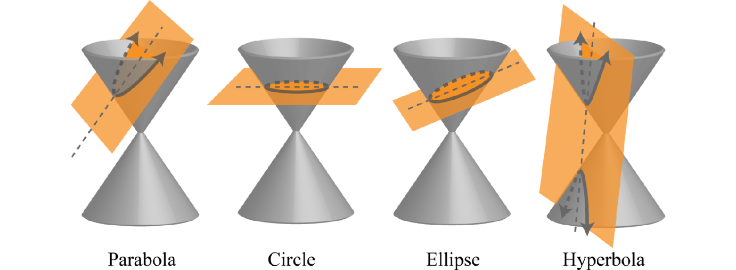
\includegraphics[scale = 0.5]{ConicSection.png}\\
(Taken from Geogebra)
\end{center}
Except parabola, others can be expressed in terms of quadratic forms. What distinguishes them is the discriminant of the quadratic equation.
\begin{proper}
Ellipses, circles, and hyperbola centered at the origin have the form of
\begin{align*}
ax^2 + bxy + cy^2 = h
\end{align*}
where $a$, $b$, $c$ and $h$ are all constants. They can be classified by the discriminant $\Delta = b^2 - 4ac$. The discriminant is positive if the graph is a hyperbola. It is negative if the graph is an ellipse (additionally $b = 0$ and $a = c$ with a circle). However, there are chances that there are no real curves regardless of the value of discriminant. They can be written as $\vec{x}^TA\vec{x} = h$, where
\begin{align*}
A &= 
\begin{bmatrix}
a & \frac{1}{2}b \\
\frac{1}{2}b & c
\end{bmatrix}
\end{align*}
Notice that the determinant $\det(A)$ is $-\frac{1}{4}$ of the discriminant.
\end{proper}
The statement above does not mention what happens when the discriminant is zero. In fact it is due to the removal of linear terms in the quadratic forms. Quadratic equations, in the most general sense, have the form of $ax^2 + bxy + cy^2 + mx + ny = h$, with $m$ and $n$ are constants as well. A zero discriminant actually represents parabola, but the lack of linear terms in quadratic terms reduces the parabola to straight lines. Of course we can include the linear terms to encompass the parabola as well, but to make our discussion below simpler, we will stick to the quadratic form expression and only talk about the central conics.\\
Short Exercise: Identify the types of curve generated by $x^2 - xy + 2y^2 = 3$ and $x^2 + xy - y^2 = 1$.
\begin{center}
\begin{tikzpicture}
\draw[thick, ->] (-3,0) -- (3,0) node[right]{$x$};
\draw[thick, ->] (0,-3) -- (0,3) node[above]{$y$};
\draw[Green,rotate=30] plot[domain=-0.8:1] ({2*cosh(\x)},{1.5*sinh(\x)});
\draw[Green,rotate=30] plot[domain=-1:0.8] ({-2*cosh(\x)},{1.5*sinh(\x)});
\draw[red,rotate=30] plot[domain=-3:3] ({\x},{0});
\draw[blue,rotate=-60] plot[domain=-3:3] ({\x},{0});
\end{tikzpicture}
\begin{tikzpicture}
\draw[thick, ->] (-3,0) -- (3,0) node[right]{$x$};
\draw[thick, ->] (0,-3) -- (0,3) node[above]{$y$};
\draw[Green, rotate=-30] (0,0) ellipse (2.5 and 1.5);
\draw[red,rotate=-30] plot[domain=-3:3] ({\x},{0});
\draw[blue,rotate=60] plot[domain=-3:3] ({\x},{0});
\end{tikzpicture} \\
Left: A hyperbola ($\frac{11}{144}x^2 + \frac{25}{24\sqrt{2}}xy - \frac{13}{48}y^2 = 1$), Right: An ellipse ($\frac{52}{225}x^2 + \frac{32}{75\sqrt{3}}xy + \frac{28}{75}y^2 = 1$). Both of them are rotated in the sense that their major axis (red) and minor axis (blue) are not aligned and made a angle of 30 degrees with the $x$ and $y$ axes. Major axis always passes through the vertices, with the minor axis perpendicular to it.
\end{center}

The last properties actually has another interpretation in terms of matrix. But before that we need to introduce some new terminologies.
\begin{defn}
For any symmetric matrix $A$, the quadratic form $\vec{x}^T A\vec{x}$ is called
\begin{enumerate}[label=(\alph*)]
\item positive definite, if for any $\vec{x} \neq \vec{0}$, $\vec{x}^T A\vec{x} > 0$ (positive semi-definite if $\vec{x}^T A\vec{x} \geq 0$), 
\item negative definite, if for any $\vec{x} \neq \vec{0}$, $\vec{x}^T A\vec{x} < 0$ (negative semi-definite if $\vec{x}^T A\vec{x} \leq 0$), 
\item indefinite if $\vec{x}^T A\vec{x}$ can take both positive and negative values,
\end{enumerate}
\end{defn}
\begin{thm}
The quadratic form $\vec{x}^T A\vec{x}$ is
\begin{enumerate}[label=(\alph*)]
\item positive definite, if and only if all eigenvalues of $A$ are positive (positive semi-definite if and only if all eigenvalues of $A$ are non-negative), 
\item negative definite, if and only if all eigenvalues of $A$ are negative (negative semi-definite if and only if all eigenvalues of $A$ are non-positive), 
\item indefinite when there are both positive and negative eigenvalues for $A$.
\end{enumerate}
\end{thm}
Now we are ready to extend our results and see what the quadratic equation $\vec{x}^TA\vec{x} = h$ can give.
\begin{thm}
Given $\vec{x}^TA\vec{x} = h$, where $h$ is chosen to be $1$ for scaling, then it represents
\begin{enumerate}[label=(\alph*)]
\item an ellipse if $A$ is positive definite,
\item a hyperbola if $A$ is indefinite,
\item no real graph if $A$ is negative definite.
\end{enumerate}
\end{thm}
For example, the quadratic equation $\vec{x}^TA\vec{x} = 1$, where
\begin{align*}
A &=
\begin{bmatrix}
1 & -2 \\
-2 & 3
\end{bmatrix}
\end{align*}
is equivalent to $x^2 - 4xy + 3y^2 = 1$. $A$ has an eigenvalue of $\lambda = 2 \pm \sqrt{5}$. As $\lambda_+ = 2 + \sqrt{5} > 0$ and $\lambda_- = 2 - \sqrt{5} < 0$, $A$ is indefinite and the curves are a pair of hyperbola.\\
\\
The figure in the last page shows that hyperbola and ellipses can be rotated. The effect on the resulted quadratic equation is to produce cross-product terms ($xy$ in two-dimensional cases), which can be eliminated by a rotation to restore the curves so that the major and minor axes are oriented along the $x$ and $y$ axes. If the graphs start with tilted by an angle of $\theta$, we can make a rotation by the same angle $\theta$ but in an opposite sense to recover the standard position. It is equivalent to rotate the coordinate system by an angle of $\theta$ in the same sense of the initial tilting. Section \ref{orthogeometricsub} can be referenced.

\begin{exmp}
Rotate the quadratic equation $x^2 - xy + y^2 = 1$ so that the major axis lies along the $x$-axis. \\
\\
First, we cast the equation into quadratic form $\vec{x}^T A\vec{x}$, with
\begin{align*}
A &=
\begin{bmatrix}
1 & -\frac{1}{2} \\
-\frac{1}{2} & 1
\end{bmatrix}
\end{align*}
We first find the eigenvalues of $A$, the characteristic equation is
\begin{align*}
(1-\lambda)^2 - (-\frac{1}{2})^2 &= 0 \\
\lambda^2 - 2\lambda + \frac{3}{4} &= 0 \\
\lambda &= \frac{1}{2} \text{ or } \frac{3}{2}
\end{align*}
So by the theorem above, $A$ is positive definite and it is an ellipse. We will see very soon the smaller eigenvalue actually corresponds to the major axis. Now we consider an orthogonal matrix $P$ to perform a rotation on the coordinate system, with the old coordinates related to the new coordinates by $\vec{x} = P\vec{x'}$. So the quadratic form is transformed to
\begin{align*}
(P\vec{x'})^T A (P\vec{x'}) &= \vec{x'}^T (P^T AP) \vec{x'}
\end{align*}
We immediately identify $P^T AP$ as a rotation of the coordinate system for the matrix $A$, as noted by the remark at the end of section \ref{orthogonaldiagreal}. The same section tells us that we can deal with the cross product terms by orthogonal diagonalization, which removes the off-diagonal entries in $A$. The normalized eigenvectors are
\begin{align*}
&\vec{v_\lambda} = \begin{bmatrix}
\frac{1}{\sqrt{2}} \\
\frac{1}{\sqrt{2}}
\end{bmatrix}
\text{ for } \lambda = \frac{1}{2}
& \begin{bmatrix}
-\frac{1}{\sqrt{2}} \\
\frac{1}{\sqrt{2}}
\end{bmatrix}
\text{ for } \lambda = \frac{3}{2}
\end{align*}
Hence we can set 
\begin{align*}
P =
\begin{bmatrix}
\frac{1}{\sqrt{2}} & -\frac{1}{\sqrt{2}} \\
\frac{1}{\sqrt{2}} & \frac{1}{\sqrt{2}}
\end{bmatrix}
\end{align*}
So that
\begin{align*}
P^T AP = 
\begin{bmatrix}
\frac{1}{\sqrt{2}} & \frac{1}{\sqrt{2}} \\
-\frac{1}{\sqrt{2}} & \frac{1}{\sqrt{2}}
\end{bmatrix}
\begin{bmatrix}
1 & -\frac{1}{2} \\
-\frac{1}{2} & 1
\end{bmatrix}
\begin{bmatrix}
\frac{1}{\sqrt{2}} & -\frac{1}{\sqrt{2}} \\
\frac{1}{\sqrt{2}} & \frac{1}{\sqrt{2}}
\end{bmatrix}
=
\begin{bmatrix}
\frac{1}{2} & 0\\
0 & \frac{3}{2}
\end{bmatrix}
= D
\end{align*}
The smaller eigenvalue is located at the first row/column, meaning now the major axis matches the new $x$-axis. The new equation is seen to be $\vec{x'}^T D\vec{x}$, or $\frac{1}{2}(x')^2 + \frac{3}{2}(y')^2 = 1$. Below are the diagrams before and after the rotation.

\begin{center}
\begin{tikzpicture}
\draw[thick, ->] (-3,0) -- (3,0) node[right](vecu){$x$};
\draw[thick, ->] (0,-3) -- (0,3) node[above]{$y$};
\draw[Green, thick, rotate=45] (0,0) ellipse ({1.2*sqrt(2)} and {1.2*sqrt(2/3)});
\draw[red, ->] (0,0) -- (2,2) node[above right](vecv){$x'$, Major axis, $\lambda = 1/2$};
\draw[blue, ->] (0,0) -- (-1,1) node[above left]{$y'$, Minor axis, $\lambda = 3/2$};
\node[Green] at (2,-2) {$x^2 - xy + y^2 = 1$};
\pic[draw, ->, "$45^\circ$", angle eccentricity=1.75] {angle = vecu--0--vecv};
\end{tikzpicture}
(Before rotation) \\
\begin{tikzpicture}
\draw[red, thick, ->] (-3,0) -- (3,0) node[right](vecu){$x'$};
\draw[blue, thick, ->] (0,-3) -- (0,3) node[above]{$y'$};
\draw[Green, thick, rotate=0] (0,0) ellipse ({1.2*sqrt(2)} and {1.2*sqrt(2/3)});
\node[Green] at (2,-2) {$\frac{1}{2}(x')^2 + \frac{3}{2}(y')^2 = 1$};
\end{tikzpicture} 
(After rotation)
\end{center}
The degree of tilting can be found to be exactly $\pi/4 = 45^{\circ}$, by comparing the general two-dimensional rotation matrix
\begin{align*}
\begin{bmatrix}
\cos \theta & -\sin \theta \\
\sin \theta & \cos \theta
\end{bmatrix}
\end{align*}
against $P$. $\cos \theta = \frac{1}{\sqrt{2}}$ and $\sin \theta = \frac{1}{\sqrt{2}}$ implies that $\tan \theta = 1$, and $\theta = \pi/4$. The possibility of eliminating the cross-product terms in quadratic forms is formally known as the Principal Axes Theorem.
\end{exmp}
\begin{thm}
For a quadratic form $\vec{x}^TA\vec{x}$, where $A$ is symmetric, we can always make an orthogonal change of variable $\vec{x'} = P^T\vec{x}$ or $\vec{x} = P\vec{x'}$ such that it turns into $\vec{x'}^TD\vec{x'} = \lambda_1 x_1'^2 + \lambda_2 x_2'^2 + \cdots$ which contains no cross-product terms. $P$ is formed by the set of orthonormal column eigenvectors of $A$ and $D$ is a diagonal matrix with entries being the eigenvalues of $A$.
\end{thm}
In general, for a two-dimensional quadratic form
\begin{align*}
\begin{bmatrix}
a & b \\
b & c
\end{bmatrix}
\end{align*}
It can undergo a rotation of the coordinate system by an angle $\theta$ such that
\begin{align*}
\begin{bmatrix}
\cos \theta & \sin \theta \\
-\sin \theta & \cos \theta
\end{bmatrix}
\begin{bmatrix}
a & b \\
b & c
\end{bmatrix}
\begin{bmatrix}
\cos \theta & -\sin \theta \\
\sin \theta & \cos \theta
\end{bmatrix}
=
\begin{bmatrix}
* & 0\\
0 & *
\end{bmatrix}
\end{align*}
the off-diagonal elements become zero. The required $\theta$ is found by  expanding the left hand side and equating both sides, which gives
\begin{align*}
-\sin \theta (a \cos\theta + b\sin \theta) + \cos\theta (b \cos \theta + c\sin \theta) &= 0 \\
\frac{c-a}{2} \sin (2\theta) + b\cos(2\theta) &= 0 \\
\cot(2\theta) &= \frac{a-c}{2b}
\end{align*}
where we apply the familiar double angle formulas.

\section{Statistics with Quadratic Form}
\subsection{Variance}
\label{variancesec}
\subsubsection{Single Distribution}
One important measure in the world of Statistics is the variance of a distribution, or a time-series. Variance can be viewed as the spread of a distribution. Below is the definition of variance for a distribution made up by one single variable.
\begin{defn}
\label{variance}
For a distribution $X$, with $n$ data $x_1, x_2, x_3, \cdots, x_n$, its population variance is
\begin{align*}
\sigma^2 = \text{Var}(X) &= \frac{1}{n} ((x_1 - \mu)^2 + (x_2 - \mu)^2 + (x_3 - \mu)^2 + \cdots + (x_n - \mu)^2) \\
&= \frac{1}{n} \sum_{k=1}^n (x_k - \mu)^2
\end{align*}
where $\mu$ is the mean, or expected value of $X$, and is computed by
\begin{align*}
\mu = E(X) = \frac{1}{n} (x_1 + x_2 + x_3 + \cdots + x_n)
\end{align*}
\end{defn}
A simpler formula for computing the population variance is
\begin{align*}
\sigma^2 = E(X^2) - (E(X))^2 = E(X^2) - \mu^2
\end{align*}
For a finite sample, we may also want to use the sample variance $s^2$, which is the population variance multiplied by a factor of $\frac{n}{n-1}$. \\
As an example, given a dataset $X$, with $5$ data $\vec{x} = (1, 3, 6, 9, 11)^T$, then the mean is
\begin{align*}
\mu = \frac{1}{5}(1 + 3 + 6 + 9 + 11) = 6
\end{align*}
and the population variance is
\begin{align*}
\sigma^2 = \frac{1}{5}((1-6)^2 + (3-6)^2 + (6-6)^2 + (9-6)^2 + (11-6)^2) = 13.6
\end{align*}
We can also use the short-cut formula.
\begin{align*}
\sigma^2 &= E(X^2) - \mu^2 \\
&= \frac{1}{5} (1^2 + 3^2 + 6^2 + 9^2 + 11^2) - 6^2 \\
&= 49.6 - 36 \\
&= 13.6
\end{align*}
Short Exercise: Find the sample variance of $X$.\\
\\
The variance formula in Definition \ref{variance} can be written in quadratic form as follows.
\begin{proper}
Given a distribution $X$, with $n$ data $\vec{x} = (x_1, x_2, x_3, \cdots, x_n)^T$, and a mean of $\mu$, the population variance can be written as
\begin{align*}
\frac{1}{n} (\vec{x'}\cdot\vec{x'}) = \frac{1}{n} \textbf{x}'^T \textbf{x}'
\end{align*}
where $\textbf{x}' = \vec{x'} = \vec{x} - \mu$ is the centered distribution with the mean $\mu$ removed. It can also be expressed as the quadratic form $\vec{x'}^T B'\vec{x'}$, where
\begin{align*}
B' &=
\begin{bmatrix}
\frac{1}{n} & 0 & 0 & \cdots \\
0 & \frac{1}{n} & 0 & \\
0 & 0 & \frac{1}{n} & \\
\vdots & & & \ddots
\end{bmatrix}
\end{align*}
is a diagonal matrix. The sample variance simply has all diagonal entries $\frac{1}{n}$ replaced by $\frac{1}{n-1}$.
\end{proper}
If we want to express the variance without involving $\mu$, then we can notice that
\begin{align*}
x'_1 &= x_1 - \frac{1}{n}(x_1 + x_2 + \cdots + x_n) = (1-\frac{1}{n})x_1 - \frac{1}{n} x_2 - \cdots - \frac{1}{n} x_n \\
x'_2 &= x_2 - \frac{1}{n}(x_1 + x_2 + \cdots + x_n) = -\frac{1}{n} x_1 + (1-\frac{1}{n}) x_2 - \cdots - \frac{1}{n} x_n \\
\cdots &= \cdots \\
x'_n &= x_n - \frac{1}{n}(x_1 + x_2 + \cdots + x_n) = -\frac{1}{n} x_1 - \frac{1}{n} x_2 - \cdots +(1-\frac{1}{n}) x_n 
\end{align*}
Hence
\begin{align*}
\vec{x'} = M\vec{x} = 
\begin{bmatrix}
1-\frac{1}{n} & -\frac{1}{n} & -\frac{1}{n} & \cdots \\
-\frac{1}{n} & 1-\frac{1}{n} & -\frac{1}{n} & \\
-\frac{1}{n} & -\frac{1}{n} & 1-\frac{1}{n} & \\
\vdots & & & \ddots
\end{bmatrix}
\vec{x}
\end{align*}
where $M$ is symmetric as well. Therefore, the desired expression is
\begin{align*}
\vec{x'}^T B'\vec{x'} &= (M\vec{x})^T B' (M\vec{x}) \\
&= \vec{x}^T (M^TB' M) \vec{x} = \vec{x}^T B \vec{x}
\end{align*}
where
\begin{align*}
B &= M^TB' M \\
&= 
\begin{bmatrix}
1-\frac{1}{n} & -\frac{1}{n} & -\frac{1}{n} & \cdots \\
-\frac{1}{n} & 1-\frac{1}{n} & -\frac{1}{n} & \\
-\frac{1}{n} & -\frac{1}{n} & 1-\frac{1}{n} & \\
\vdots & & & \ddots
\end{bmatrix}
\begin{bmatrix}
\frac{1}{n} & 0 & 0 & \cdots \\
0 & \frac{1}{n} & 0 & \\
0 & 0 & \frac{1}{n} & \\
\vdots & & & \ddots
\end{bmatrix}
\begin{bmatrix}
1-\frac{1}{n} & -\frac{1}{n} & -\frac{1}{n} & \cdots \\
-\frac{1}{n} & 1-\frac{1}{n} & -\frac{1}{n} & \\
-\frac{1}{n} & -\frac{1}{n} & 1-\frac{1}{n} & \\
\vdots & & & \ddots
\end{bmatrix} \\
&= \frac{1}{n}
\begin{bmatrix}
1-\frac{1}{n} & -\frac{1}{n} & -\frac{1}{n} & \cdots \\
-\frac{1}{n} & 1-\frac{1}{n} & -\frac{1}{n} & \\
-\frac{1}{n} & -\frac{1}{n} & 1-\frac{1}{n} & \\
\vdots & & & \ddots
\end{bmatrix} 
\begin{bmatrix}
1-\frac{1}{n} & -\frac{1}{n} & -\frac{1}{n} & \cdots \\
-\frac{1}{n} & 1-\frac{1}{n} & -\frac{1}{n} & \\
-\frac{1}{n} & -\frac{1}{n} & 1-\frac{1}{n} & \\
\vdots & & & \ddots
\end{bmatrix} \\
&= 
\frac{1}{n}
\begin{bmatrix}
1-\frac{1}{n} & -\frac{1}{n} & -\frac{1}{n} & \cdots \\
-\frac{1}{n} & 1-\frac{1}{n} & -\frac{1}{n} & \\
-\frac{1}{n} & -\frac{1}{n} & 1-\frac{1}{n} & \\
\vdots & & & \ddots
\end{bmatrix} =
\begin{bmatrix}
\frac{n-1}{n^2} & -\frac{1}{n^2} & -\frac{1}{n^2} & \cdots \\
 -\frac{1}{n^2} & \frac{n-1}{n^2} & -\frac{1}{n^2} & \\
 -\frac{1}{n^2} & -\frac{1}{n^2} & \frac{n-1}{n^2} & \\
\vdots & & & \ddots
\end{bmatrix}
\end{align*}
The readers are invited to verify that $M^TM = M^2 = M$ as shown in the calculation above. To obtain the sample variance, multiply the whole expression by the factor $\frac{n}{n-1}$. Also, due to the nature of variance that it can never be negative, $B$ is positive semi-definite.\\
Short Exercise: Discuss under what situation the variance will be zero.

\subsubsection{Linear Combination of Multiple Distributions}
Sometimes we may need to consider the distribution of the sum of multiple variables. More generally, given any linear combination of multiple distributions, like $Z = c_1X^{(1)} + c_2X^{(2)} + \cdots + c_nX^{(n)}$, we may want to know about its mean and variance. The mean will be simply $\mu_Z = c_1\mu_1 + c_2\mu_2 + \cdots + c_n\mu_n$, where $\mu_j$ is the mean of $X^{(j)}$. The variance $\text{Var}(Z)$ is a bit more complicated. First, we need to introduce the concept of covariance between any two distributions, which is
\begin{defn}
\label{covariance}
For two distributions $X$ and $Y$, each with $n$ pairs of members, their population covariance is
\begin{align*}
\text{Cov}(X,Y) &= \frac{1}{n}((x_1-\mu_x)(y_1-\mu_y) + (x_2-\mu_x)(y_2-\mu_y)) + \cdots + (x_n-\mu_x)(y_n-\mu_y)) \\
&= \frac{1}{n}\sum_{k=1}^{n} (x_k-\mu_x)(y_k-\mu_y)
\end{align*}
where $\mu_x$ and $\mu_y$ are the population means of $X$ and $Y$ respectively. The order does not matter, as $\text{Cov}(X,Y) = \text{Cov}(Y,X)$. If $\vec{x'}$ and $\vec{y'}$ are the centered data with their mean subtracted away, then it can be denoted by the vector notation as
\begin{align*}
\frac{1}{n} \vec{x'} \cdot \vec{y'} = \frac{1}{n} \textbf{x}'^T \textbf{y}'
\end{align*}
For sample covariance, it is
\begin{align*}
q_{xy} = \frac{1}{n-1} \sum_{k=1}^{n} (x_k-\bar{x})(y_k-\bar{y})
\end{align*}
where $\bar{x}$ and $\bar{y}$ are the sample means of $X$ and $Y$ which happen to have the same values as $\mu_x$ and $\mu_y$.
\end{defn}
There are short-cut formula similar as that for variance. The population covariance can be computed as
\begin{align*}
\text{Cov}(X,Y) &= E(XY) - E(X)E(Y)    
\end{align*}
The sample covariance has an additional factor of $\frac{n}{n-1}$. Also, a direct comparison reveals that $\text{Cov}(X,X) = \text{Var}(X)$ for any distribution $X$.

\begin{exmp}
Two time-series of zonal and meridional wind speed $U$ and $V$, have measurements as shown in the table below.
\begin{center}
\begin{tabular}{|c|c|c|}
\hline
(in \si{\m \per \s}) & $U$ & $V$\\
\hline
1st Measurement & 4 & -3 \\
\hline
2nd Measurement & 3 & -1 \\
\hline
3nd Measurement & 3 & -2 \\
\hline
4th Measurement & 2 & -1 \\
\hline
\end{tabular}
\end{center}
Find the covariance of $U$ and $V$.\\
It is not hard to get $\mu_u = 3$ and $\mu_v = -\frac{7}{4}$. From the definition, we have
\begin{align*}
\text{Cov}(U,V) &= \frac{1}{4} [(4-3)((-3)-(-1.75))+(3-3)((-1)-(-1.75)) \\
&\quad+(3-3)((-2)-(-1.75))+(2-3)((-1)-(-1.75))] \\
&= \SI{-0.5}{\square\m \per \square\s}
\end{align*}
Alternatively, the short-cut formula gives
\begin{align*}
\text{Cov}(U,V) &= E(UV) - \mu_u \mu_v \\
&= \frac{1}{4}((4)(-3) + (3)(-1) + (3)(-2) + (2)(-1)) - (3)(-\frac{7}{4}) \\
&= (-5.75) - (-5.25) = \SI{-0.5}{\square\m \per \square\s}
\end{align*}
\end{exmp}
Remember we use the formula for population covariance, and we have to scale by an appropriate factor when computing the sample covariance. From the example, we can make two observations. First, if $X$ and $Y$ both have the same unit $a$, then the unit of their covariance, or the variance for each of them individually, have the unit of $a^2$. Also, covariance can take negative values, which is different from variance which is always non-negative.\\
\\
Another useful measure related to variance and covariance is correlation. For two distribution $X$ and $Y$, the correlation is defined by the following formula.
\begin{defn}
The correlation of two distributions $X$ and $Y$ is
\begin{align*}
\rho_{xy} &= \frac{\text{Cov}(X,Y)}{\sqrt{\text{Var}(X) \text{Var}(Y)}} \\
&= \frac{\text{Cov}(X,Y)}{\sqrt{\text{Cov}(X,X) \text{Cov}(Y,Y)}}
\end{align*}
\end{defn}
Moreover,
\begin{defn}
The correlation between any two distributions $X$ and $Y$ falls in the range of $-1$ and $1$, i.e. $-1 \leq \rho_{xy} \leq 1$.
\paragraph{Proof} We can rewrite the correlation using vector notation for covariance, which gives
\begin{align*}
\rho_{xy} &= \frac{(\vec{x'} \cdot \vec{y'})}{\sqrt{(\vec{x'}\cdot\vec{x'})(\vec{y'}\cdot\vec{y'})}} \\
&= \frac{(\vec{x'} \cdot \vec{y'})}{\sqrt{{\norm{\vec{x'}}}\norm{\vec{y'}}}}
\end{align*}
where $\vec{x'}$ and $\vec{y'}$ are centered by removing the mean from the original distributions. By comparing to Cauchy-Schwarz Inequality proved in Theorem \ref{CauchySch}, we promptly know that $\abs{\rho_{xy}} \leq 1$.
\end{defn}
Correlation between two distributions $X$ and $Y$ indicates how their data varies together in a linear fashion. If the correlation is positive, then $X$ and $Y$ will increase or decrease together. However, if the correlation is negative, then when one of them increases, one of them will decrease, and vice versa. Higher the correlation, stronger the relationship. If the correlation is close to zero, it means that there are no clear linear relationship between them, however this does not exclude the possibility of having other relationship, e.g. exponential.
\begin{center}
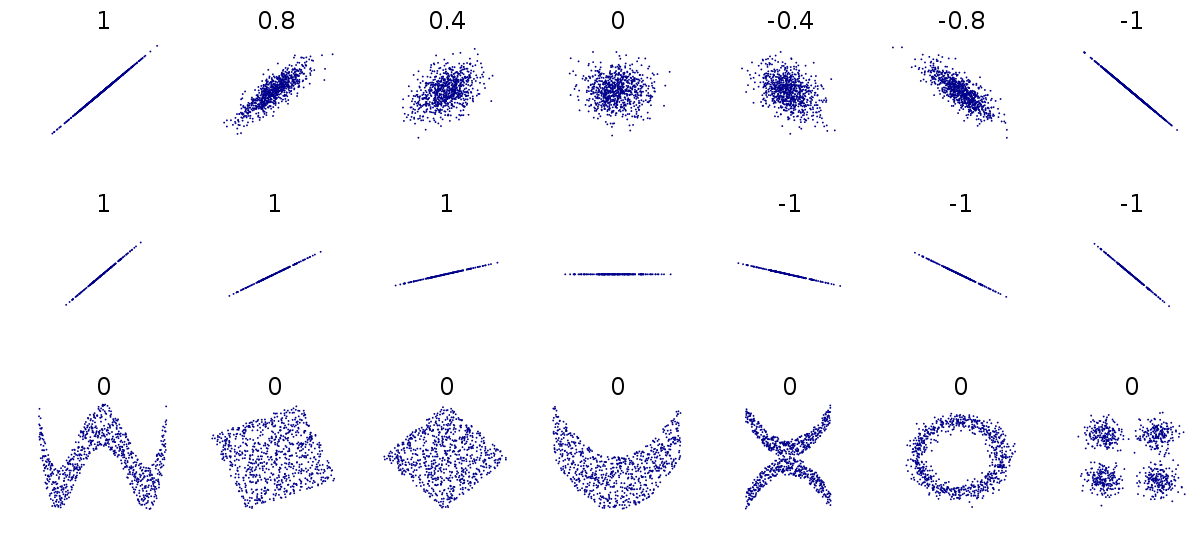
\includegraphics[scale = 0.3]{1200px-Correlation_examples2.svg.png}\\
(Taken from Wikipedia)
\end{center}
In the last example, $\text{Cov}(U,V) = \SI{-0.5}{\square\m \per \square\s}$, $\text{Var}(U) = \SI{0.5}{\square\m \per \square\s}$,\\
$\text{Var}(V) = \SI{0.6875}{\square\m \per \square\s}$, and $\rho_{uv} = \frac{0.5}{\sqrt{(0.5)(0.6875)}} \approx -0.8528$. We use the population variance and covariance for the computation, but they can be replaced by the sample counterparts at once. It may be tempting to claim that a strong negative relationship exists in this case. However, we note that the sample size here is a bit small for this result to be meaningful. Also, correlation is always dimensionless.\\
\\
We are now prepared to derive the variance formula for linear combinations of multiple variables.
\begin{proper}
\label{variancemul}
For a distribution made up of multiple variables, in the form of $Z = c_1X^{(1)} + c_2X^{(2)} + \cdots + c_nX^{(n)}$, with $\vec{c} = (c_1, c_2, \cdots, c_n)^T$ are all constants, the population variance $\text{Var}(Z)$ can be expressed as a quadratic form $\vec{c}^TQ\vec{c}$, where
\begin{align*}
Q &=
\begin{bmatrix}
\text{Cov}(X^{(1)}, X^{(1)}) & \text{Cov}(X^{(1)}, X^{(2)}) & \cdots & \text{Cov}(X^{(1)}, X^{(n)}) \\
\text{Cov}(X^{(2)}, X^{(1)}) & \text{Cov}(X^{(2)}, X^{(2)}) & \cdots & \text{Cov}(X^{(2)}, X^{(n)}) \\
\vdots & \vdots &  & \vdots \\
\text{Cov}(X^{(n)}, X^{(1)}) & \text{Cov}(X^{(n)}, X^{(2)}) & \cdots & \text{Cov}(X^{(n)}, X^{(n)}) \\
\end{bmatrix} \\
&=
\begin{bmatrix}
\text{Var}(X^{(1)}) & \text{Cov}(X^{(1)}, X^{(2)}) & \cdots & \text{Cov}(X^{(1)}, X^{(n)}) \\
\text{Cov}(X^{(2)}, X^{(1)}) & \text{Var}(X^{(2)}) & \cdots & \text{Cov}(X^{(2)}, X^{(n)}) \\
\vdots & \vdots &  & \vdots \\
\text{Cov}(X^{(n)}, X^{(1)}) & \text{Cov}(X^{(n)}, X^{(2)}) & \cdots & \text{Var}(X^{(n)}) \\
\end{bmatrix} 
\end{align*}
is the so-called covariance matrix. If $[X'] = [X'^{(1)}|X'^{(2)}|\cdots|X'^{(n)}]$ is consisted of the centered variables in columns, then $Q = \frac{1}{n}X'^TX$. To find the sample variance of $Z$, replace all $\text{Cov}(X^{(i)}, X^{(j)})$ by $q_{ij}$ in Definition \ref{covariance}.
\paragraph{Proof} To allow easier understanding, we will deal with the case of $n = 2$. However, the idea can be extended for other values of $n$. Starting from the expression in Definition \ref{variance}, we have
\begin{align*}
\text{Var}(Z) &= \frac{1}{n} \sum_{k=1}^n (z_k - \mu_z)^2 \\
&= \frac{1}{n} \sum_{k=1}^n ((c_1X^{(1)}_k + c_2X^{(2)}_k) - (c_1\mu_{x_1} + c_2\mu_{x_2}))^2 \\
&= \frac{1}{n} \sum_{k=1}^n (c_1(X^{(1)}_k - \mu_{x_1}) + c_2(X^{(2)}_k - \mu_{x_2}))^2 \\
&= \frac{1}{n} c_1^2 \sum_{k=1}^n (X^{(1)}_k - \mu_{x_1})^2 + \frac{1}{n} c_2^2 \sum_{k=1}^n (X^{(2)}_k - \mu_{x_2})^2 \\
&\quad+ \frac{2}{n} c_1c_2 \sum_{k=1}^n (X^{(1)}_k - \mu_{x_1}) (X^{(2)}_k - \mu_{x_2}) \\
&= c_1^2 \text{Cov}(X^{(1)}, X^{(1)}) + c_2^2 \text{Cov}(X^{(2)}, X^{(2)}) + 2c_1c_2 \text{Cov}(X^{(1)}, X^{(2)}) \\
&= c_1^2 \text{Cov}(X^{(1)}, X^{(1)}) + c_1c_2 \text{Cov}(X^{(1)}, X^{(2)}) \\
&\quad + c_2c_1 \text{Cov}(X^{(2)}, X^{(1)}) + c_2^2 \text{Cov}(X^{(2)}, X^{(2)}) \\
&= \sum_{i=1}^{n=2}\sum_{j=1}^{n=2} c_ic_j\text{Cov}(X^{(i)}, X^{(j)})
\end{align*}
where the terms are identified by Definition \ref{covariance}. By comparing to Definition \ref{quadform}, we realize the expression is simply
\begin{align*}
\vec{c}^TQ\vec{c} =
\begin{bmatrix}
c_1 & c_2
\end{bmatrix}
\begin{bmatrix}
\text{Cov}(X^{(1)}, X^{(1)}) & \text{Cov}(X^{(1)}, X^{(2)}) \\
\text{Cov}(X^{(2)}, X^{(1)}) & \text{Cov}(X^{(2)}, X^{(2)}) 
\end{bmatrix}
\begin{bmatrix}
c_1 \\
c_2
\end{bmatrix}
\end{align*}
for two variables situation.
\end{proper}

\begin{exmp}
From the previous wind speed example, if $W = 0.8U-0.6V$, find $\text{Var}(W)$.\\
\\
Earlier calculations show $\text{Var}(U) = \SI{0.5}{\square\m \per \square\s}$,
$\text{Var}(V) = \SI{0.6875}{\square\m \per \square\s}$, $\text{Cov}(U,V) = \text{Cov}(V,U) = \SI{-0.5}{\square\m \per \square\s}$. Plugging the values into the expression we just get, we have
\begin{align*}
\text{Var}(W) &=
\begin{bmatrix}
c_u & c_v
\end{bmatrix}
\begin{bmatrix}
\text{Var}(U) & \text{Cov}(U,V) \\
\text{Cov}(U,V) & \text{Var}(V)
\end{bmatrix}
\begin{bmatrix}
c_u \\
c_v
\end{bmatrix} \\
&=
\begin{bmatrix}
0.8 & -0.6
\end{bmatrix}
\begin{bmatrix}
0.5 & -0.5 \\
-0.5 & 0.6875
\end{bmatrix}
\begin{bmatrix}
0.8 \\
-0.6
\end{bmatrix} \\
&= \SI{1.0475}{\square\m \per \square\s}
\end{align*}
\end{exmp}

\subsection{Principal Component Analysis}
A common practice in Earth Science is to reduce the dimensions of a large set of data. Given a large number of variables, each with a substantial amount of measurements, we want to process them to extract and retain the most important features or signals. Principal Component Analysis, which also known as Empirical Orthogonal Function in atmospheric science, is the mainstream method to achieve this goal, by finding the pattern which maximizes the variance of the dataset. It will be explained slowly with some diagrams and helper theorems.\\
\\
Consider the simplest case with two variables, or time-series $X$ and $Y$ first. Assume they have $n$ pairs of entries, from $\vec{x_1}^T = (x_1, y_1)^T$ to $\vec{x_n}^T = (x_{n}, y_{n})^T$. We can compute the covariance matrix $Q$, introduced in the last section. Principal Component Analysis want to find a unit vector $\textbf{e}$, so that the variance of data along the direction indicated by $\textbf{e}$, which is $\textbf{e}^T Q \textbf{e}$ following from Properties \ref{variancemul}, is maximized.
\begin{center}
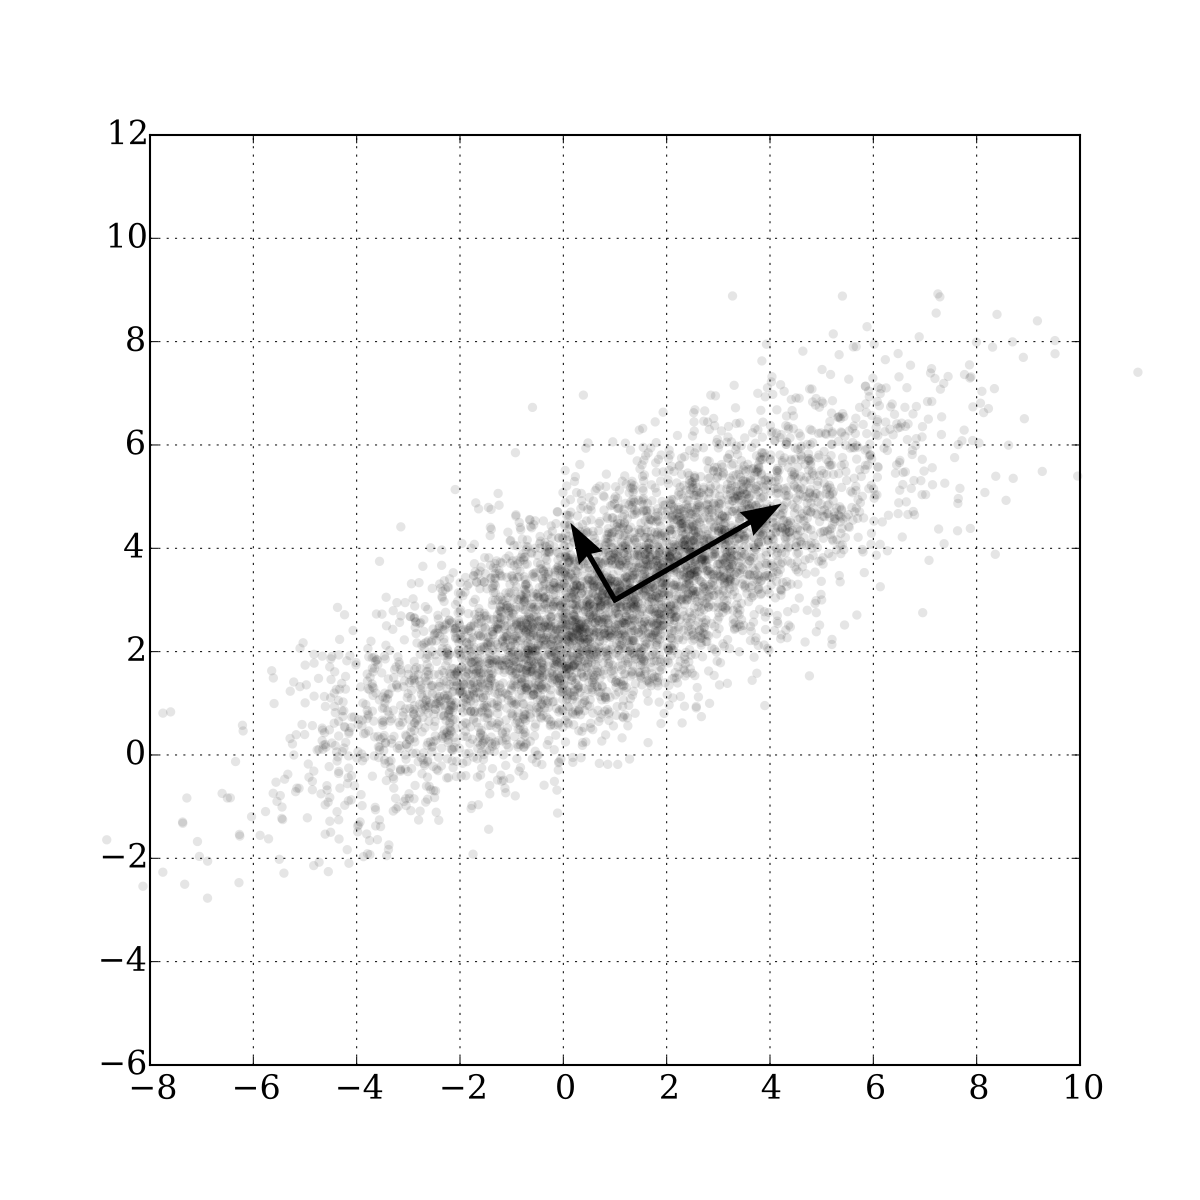
\includegraphics[scale = 0.15]{1200px-GaussianScatterPCA.svg.png}\\
Two principal axes found by Principal Component Analysis for a set of data. The longer vector represents the direction of largest variance. The data points can be seen to spread more along that direction. (Taken from Wikipedia)
\end{center}
Now the problem is to find, under what situation $\textbf{e}^T Q \textbf{e}$ will assume its largest value. Here, we introduce a famous technique, called the Lagrange Multiplier, which requires some knowledge in Calculus. As before, we will proceed with the 2 variables case for brevity.
\begin{thm}
\label{LagrangeMul}
To find the extremal values attained by a function $f(u,v,\cdots)$, under the constraint $g(u,v,\cdots) = 0$, we consider the expression
\begin{align*}
h(u,v,\cdots) = f(u,v,\cdots) - \lambda g(u,v,\cdots)
\end{align*}
where $\lambda$ is a constant to be determined by solving the system
\begin{align*}
\begin{cases}
\partial h/\partial u &= 0 \\
\partial h/\partial v &= 0 \\
\cdots &= 0
\end{cases}
\end{align*}
$\partial/\partial u$ and $\partial/\partial v$ means differentiating with $u$ and $v$ only while treating other variables as constants. The values of $u$ and $v$ to reach the extremums are also inferred from the set of equations above. 
\end{thm}
We are now going to find the value of $x'$ and $y'$ so that $\textbf{e}^T Q \textbf{e}$ obtains the maximum for $\textbf{e}^T = (x',y')$. The constraint is that $\textbf{e}$ is a unit vector as a direction, and hence by the method of Lagrange Multiplier outlined in Theorem \ref{LagrangeMul}, we have
\begin{align*}
g(x',y') = x'^2 + y'^2 - 1 = 0
\end{align*}
and with $f(x',y') = \textbf{e}^T Q \textbf{e}$
\begin{align*}
h(x',y') &= (\textbf{e}^T Q \textbf{e}) - \lambda(x'^2 + y'^2 - 1) \\
&= x'^2 \text{Cov}(X, X) + 2x'y' \text{Cov}(X, Y) + y'^2\text{Cov}(Y, Y) - \lambda(x'^2 + y'^2 - 1)
\end{align*}
according to Properties \ref{variancemul}. Carrying out the differentiation gives
\begin{align*}
\begin{cases}
\partial h/\partial x' &= 2x'\text{Cov}(X, X) + 2y'\text{Cov}(X, Y) - 2\lambda x' = 0 \\
\partial h/\partial y' &= 2x'\text{Cov}(X, Y) + 2y'\text{Cov}(Y, Y) - 2\lambda y' = 0
\end{cases}    
\end{align*}
This system can be immediately be recognised as
\begin{align*}
\begin{bmatrix}
\text{Cov}(X, X)-\lambda & \text{Cov}(X, Y) \\
\text{Cov}(Y, X) & \text{Cov}(Y, Y)-\lambda
\end{bmatrix}
\begin{bmatrix}
x' \\
y'
\end{bmatrix} &= 0\\
(Q-\lambda I)\vec{x'} &= 0
\end{align*}
which is an eigenvalue problem like those in Section \ref{eigensection}. Hence we conclude that $f(x',y') = \textbf{e}^T Q \textbf{e}$ attains its extremal values when $\textbf{e}^T = (x',y')^T$ is the unit eigenvector of $Q$. The corresponding magnitude of variance ${\textbf{e}^{(j)}}^T Q \textbf{e}^{(j)}$ for the $j$-th eigenvector is
\begin{align*}
{\textbf{e}^{(j)}}^T (Q \textbf{e}^{(j)}) &= {\textbf{e}^{(j)}}^T (\lambda^{(j)} \textbf{e}^{(j)}) \\
&= \lambda^{(j)} ({\textbf{e}^{(j)}}^T \textbf{e}^{(j)}) \\
&= \lambda^{(j)} (\hat{e}^{(j)} \cdot \hat{e}^{(j)}) \\
&= \lambda^{(j)} \norm{\hat{e}^{(j)}} \\
&= \lambda^{(j)}
\end{align*}
where we have used the facts that $Q \textbf{e}^{(j)} = \lambda^{(j)} \textbf{e}^{(j)}$ as per Definition \ref{eigen} and the length of a unit vector is $1$. This means that the variance along the direction of eigenvector is exactly the corresponding eigenvalue. To generalize for more variables, we have the following results.
\begin{thm}
For a covariance matrix $Q$ which happens to be symmetric, the variance $\textbf{e}^T Q \textbf{e}$ achieves its maximum value $\lambda_1$ along the direction $\textbf{e}^{(1)}$, which are the largest eigenvalue of $Q$ and the associated unit eigenvector. \\
Generally, if $Q$ has the orthonormal eigenvectors $\textbf{e}^{(1)}, \textbf{e}^{(2)}, \cdots, \textbf{e}^{(n)}$, arranged by the eigenvalues $\lambda_1 > \lambda_2 > \cdots > \lambda_n$, then the largest variance will be $\lambda_1$ when the direction is along $\textbf{e}^{(1)}$, the second largest will be  $\lambda_2$ for $\textbf{e}^{(2)}$ and so on, with the smallest variance being $\lambda_n$ for $\textbf{e}^{(n)}$. This set of linearly independent eigenvectors are called the Principal Directions in Principal Component Analysis.
\end{thm}
As a side note, any quadratic form $\hat{x}^TA\hat{x}$ will attain its maximum and minimum when $\hat{x}$ is the eigenvector that represents the largest and smallest eigenvalue, which are also the value $\hat{x}^TA\hat{x}$ takes when it happens. This is under the constraint that $\hat{x}$ is a unit vector, and has the name Constrained Extremum Theorem.\\
\\
Going back to the problem of Principal Component Analysis, for each Principal Directions $\textbf{e}^{(j)}$ and the variance $\lambda_{j}$, we can compute the ratio of explained variance, which is the fraction $\lambda_{j}$ over the total variance, that is the sum of eigenvalues for the covariance matrix. This number allows us to access how well the Principal Direction contributes to the total variance.\\
\\
With the set of orthonormal principal directions at hand, we can treat them as a coordinate basis and subsequently perform a rotation on the data as we have done earlier. Constructing a transition matrix made up of the Principal Directions $[\textbf{e}] = [\textbf{e}^{(1)}|\textbf{e}^{(2)}|\cdots|\textbf{e}^{(n)}]$, the new coordinates are $\vec{u} = [\textbf{e}]^T \vec{x}$ as suggested by Section \ref{orthogeometricsub}. $\vec{u_i}$ can be regarded to be the projection of $\vec{x_i}^T = (x_i, y_i)^T$ the $i$-th pair of data onto the principal directions and is called the Principal Components. By doing an orthogonal rotation on $Q$ by $[\textbf{e}]$, the resulted quantities $[\textbf{e}]^T Q[\textbf{e}]$ will be a diagonal matrix with non-trivial elements being the variances along the Principal Directions. \\
\\
Usually, at the start we will detrend the data and remove the mean from each variable, such that we use $x'_i = x_i - \bar{x}$ and $y'_i = y_i - \bar{y}$ to replace $x_i$ and $y_i$.

\begin{exmp}
The temperature data of two cities $M$ and $N$ are as follows.
\begin{center}
\begin{tabular}{|c|c|c|}
\hline
(in \si{\degree C}) & $M$ & $N$\\
\hline
1st Day & 22.1 & 22.3 \\
\hline
2nd Day & 21.8 & 21.6 \\
\hline
3nd Day & 20.9 & 21.2 \\
\hline
4th Day & 21.6 & 21.7 \\
\hline
5th Day & 23.4 & 23.2 \\
\hline 
6th Day & 24.7 & 24.1 \\
\hline 
7th Day & 22.0 & 23.9 \\
\hline 
8th Day & 22.1 & 22.4 \\
\hline 
\end{tabular}
\end{center}
Perform Principal Component Analysis and find the strongest Principal Direction, and extract the time-series related to this mode.\\
\\
After detrending, the data are
\begin{center}
\begin{tabular}{|c|c|c|}
\hline
(in \si{\degree C}) & $M'$ & $N'$\\
\hline
1st Day & -0.225 & -0.25 \\
\hline
2nd Day & -0.525 & -0.95 \\
\hline
3nd Day & -1.425 & -1.35 \\
\hline
4th Day & -0.725 & -0.85 \\
\hline
5th Day & 1.075 & 0.65 \\
\hline 
6th Day & 2.375 & 1.55 \\
\hline 
7th Day & -0.325 & 1.35 \\
\hline 
8th Day & -0.225 & -0.15 \\
\hline 
\end{tabular}
\end{center}
From Properties \ref{variancemul}, the sample covariance matrix is
\begin{align*}
Q = 
\frac{1}{8-1}
\begin{bmatrix}
\vec{m'}\cdot\vec{m'} & \vec{m'}\cdot\vec{n'} \\
\vec{n'}\cdot\vec{m'} & \vec{n'}\cdot\vec{n'} 
\end{bmatrix} =
\begin{bmatrix}
1.405 & 1.01 \\
1.01 & 1.1686
\end{bmatrix}
\end{align*}
The unit eigenvectors for $Q$ and thus the Principal Directions can be found to be $\textbf{e}^{(1)} = (0.747, -0.665)^T$ of larger variance $\lambda_1 = \SI{2.304}{\square {(\degree C)}}$, and $\textbf{e}^{(2)} = (0.665, 0.747)^T$ of smaller variance $\lambda_2 = \SI{0.270}{\square {(\degree C)}}$. The first principal component accounts for $2.304 / (2.304+0.270) \approx 89.5\%$ of the total variance.\\
\\
We can project every pair of data $\vec{x'}_i^T = (m'_i, n'_i)^T$ onto the principal directions by computing $\vec{u}_i = [\textbf{e}]^T\vec{x'}_i$, where $[\textbf{e}] = [\textbf{e}^{(1)}|\textbf{e}^{(2)}]$. The principal values are 
\begin{center}
\begin{tabular}{|c|c|c|c|c|c|c|c|c|}
\hline
(in \si{\degree C}) & D-1 & D-2 & D-3 & D-4 & D-5 & D-6 & D-7 & D-8 \\
\hline
$u^{(1)}$ & -0.334 & -1.024 & -1.962 & -1.107 & 1.235 & 2.805 & 0.655 & -0.268 \\
\hline
$u^{(2)}$ & -0.037 & -0.361 & -0.061 & -0.153 & -0.229 & -0.421 & 1.225 & 0.038 \\
\hline
\end{tabular}
\end{center}
In details, the principal components for the first day is computed by
\begin{align*}
\begin{bmatrix}
u_1^{(1)} \\
u_1^{(2)} 
\end{bmatrix}
=
\begin{bmatrix}
0.747 & 0.665 \\
-0.665 & 0.747
\end{bmatrix}
\begin{bmatrix}
-0.225 \\
-0.25
\end{bmatrix}
\end{align*}
The original dataset can be recovered by $\vec{x'}_i = [\textbf{e}]\vec{u'}_i$. If we want to extract the signals originated from the first Principal Directions, we can simply remove other column eigenvectors in $[\textbf{e}]$ and discard other principal values in $\vec{u'}_i$. The time-series reconstructed by the first mode is hence computed by $x'_i = \textbf{e}^{(1)}u_i^{(1)}$, which are
\begin{center}
\begin{tabular}{|c|c|c|c|c|c|c|c|c|}
\hline
(in \si{\degree C}) & D-1 & D-2 & D-3 & D-4 & D-5 & D-6 & D-7 & D-8 \\
\hline
$M'$ & -0.250 & -0.765 & -1.466 & -0.827 & 0.923 & 2.095 & 0.489 & -0.200 \\
\hline
$N'$ & -0.222 & -0.681 & -1.304 & -0.736 & 0.821 & 1.864 & 0.435 & -0.178 \\
\hline
\end{tabular}
\end{center}
\end{exmp}
\newpage
\begin{center}
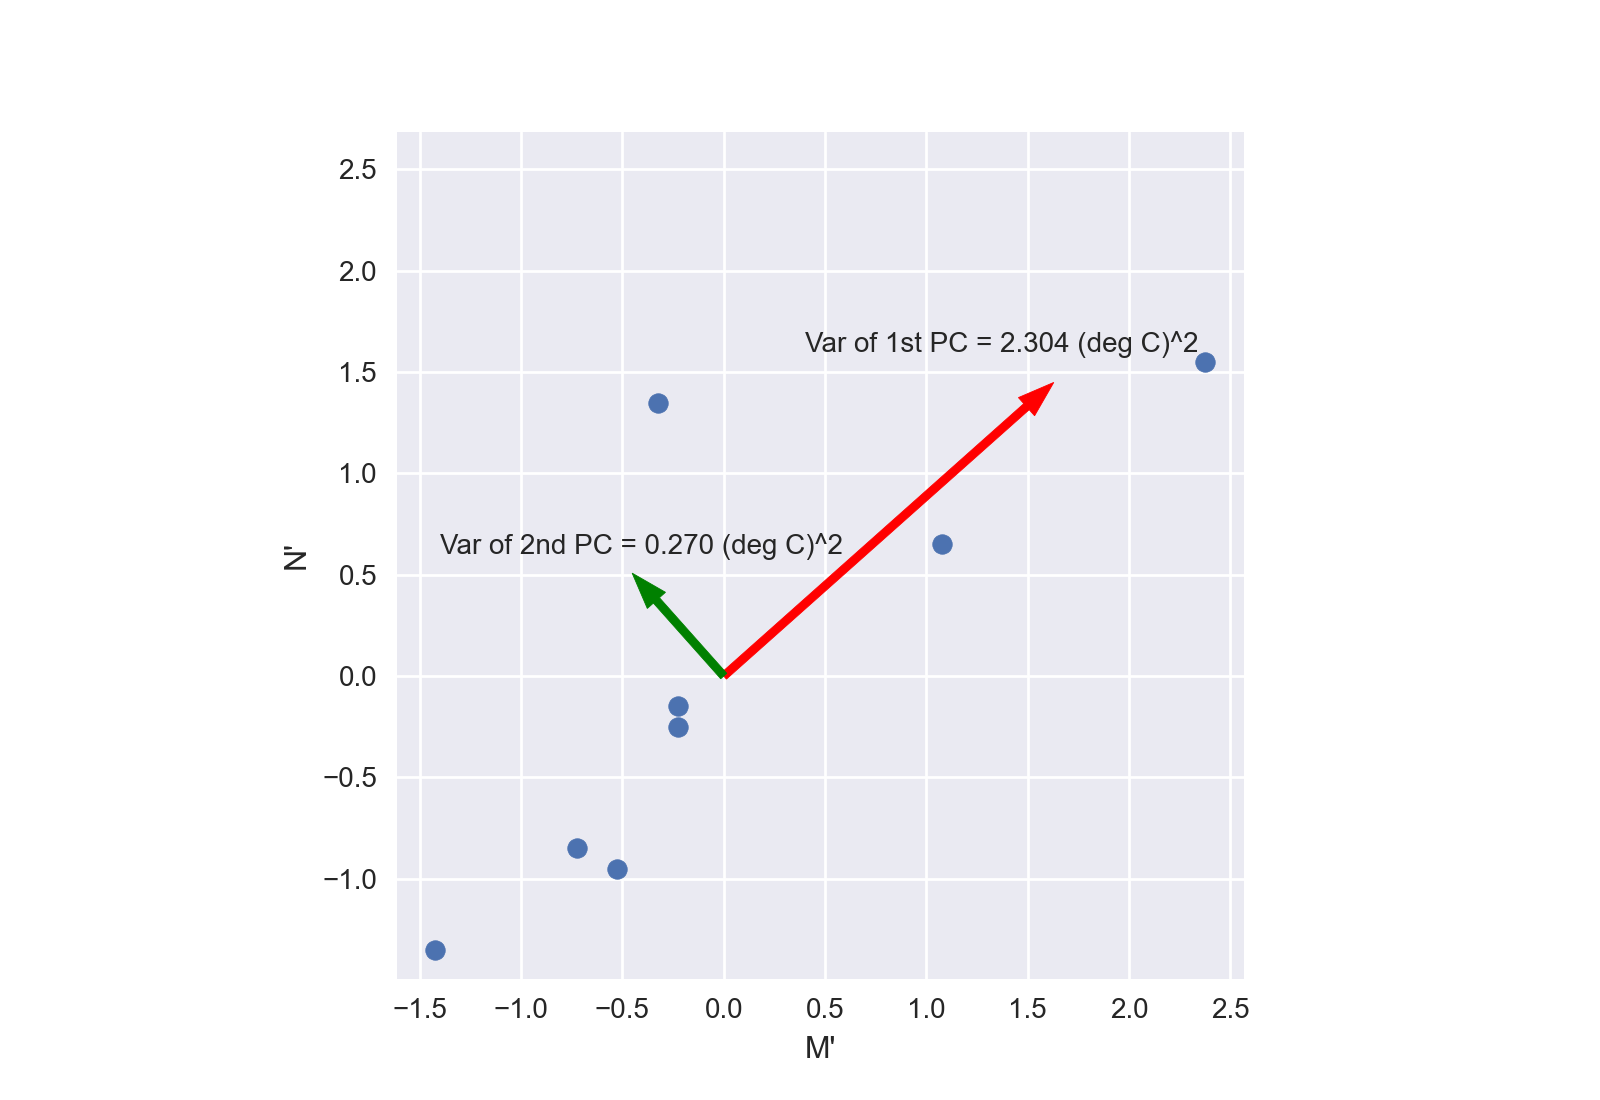
\includegraphics[scale = 0.6]{LAEOF.png}\\
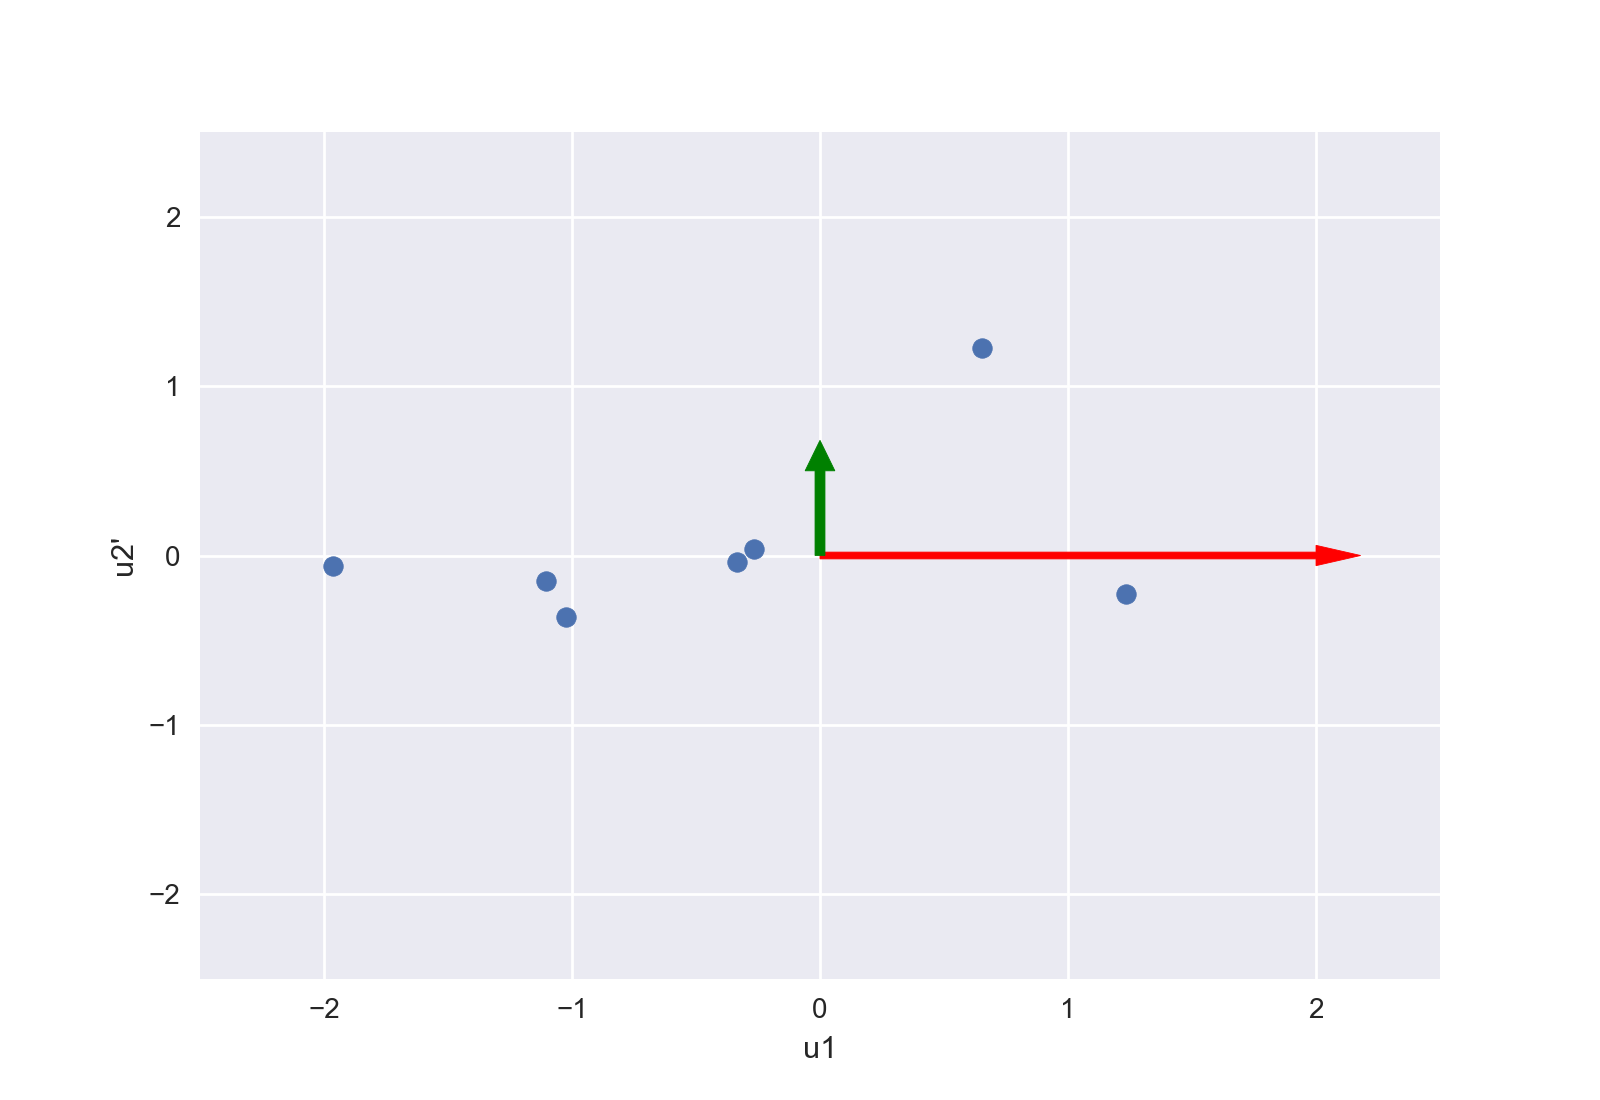
\includegraphics[scale = 0.6]{LAEOF2.png}\\
The data before and after rotation by the principal directions, with the one with larger/smaller variance shown as red/green.
\end{center}
\begin{center}
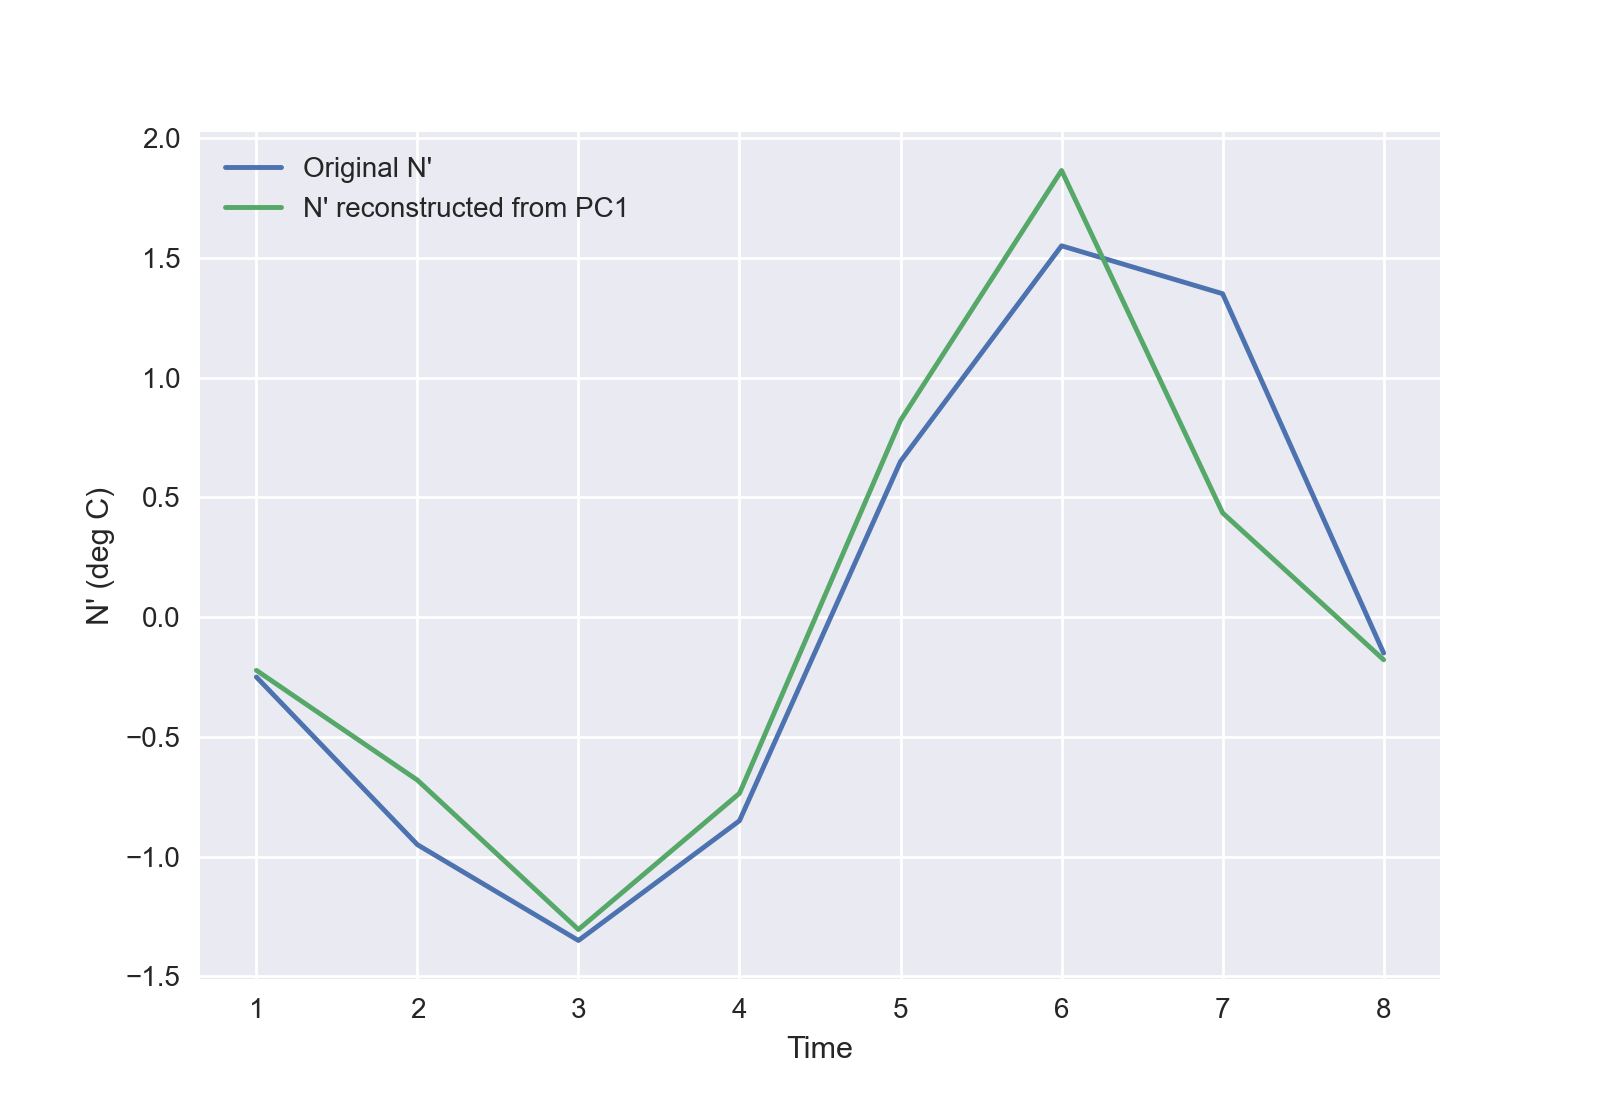
\includegraphics[scale = 0.6]{LAEOF3.png}\\
Comparison between the original anomaly and the first mode for $N'$.
\end{center}

\section{Exercise}

\begin{Exercise}
Identify the following conic sections and eliminate the cross-product terms by an appropriate rotation.
\begin{enumerate}[label=(\alph*)]
\item $x^2 + 5xy + 3y^2 = 1$,
\item $x^2 - xy + 2y^2 = 4$,
\item $x^2 + 2xy + y^2 = 1$, what is the curve generated? 
\end{enumerate}
\end{Exercise}

\begin{Exercise}
Find a new expression for the standard hyperbola $y^2 - x^2 = 1$ if a anti-clockwise rotation of $75$ degrees is done. What about a reflection along the $x$-axis?
\end{Exercise}

\begin{Exercise}
Three-dimensional quadrics can also be treated in a similar fashion to two-dimensional conic sections. Find the length of three axes for an ellipsoid $x^2 + y^2 + z^2 + 0.5xy - yz + 0.5xz = 1$ by doing an orthogonal coordinate transformation. What is the requirement for a three-dimensional quadratic form to represent an ellipsoid?
\end{Exercise}

\begin{Exercise}
Find the covariance matrix for three pressure time-series over $10$ days at cities $X$, $Y$, $Z$ (in hPa, relative to $1000$ hPa), which take the values
\begin{center}
\begin{tabular}{|c|c|c|}
\hline
$X$ & $Y$ & $Z$ \\
\hline
17 & 19 & 22 \\
\hline
18 & 16 & 25 \\
\hline
14 & 15 & 17 \\
\hline
19 & 21 & 23 \\
\hline
24 & 22 & 26 \\
\hline
21 & 20 & 23 \\
\hline 
28 & 26 & 29 \\
\hline
24 & 25 & 22 \\
\hline
20 & 21 & 27 \\
\hline
23 & 22 & 24 \\
\hline
\end{tabular}
\end{center}
Find the variance of $W = X - 0.5Y - 0.5Z$.
\end{Exercise}

\begin{Exercise}
Carry out Principal Component Analysis on the data set above. Find the Principal Directions and the ratio of explained variance for each of them. Reconstruct the data using the first Principal Direction with largest variance only.
\end{Exercise}


\chapter{Least-Square Approximation}

\section{Mathematical Ideas of Least-Square Approximation}

As discussed in Chapter \ref{chap:SolLinSys}, given a linear system $A\vec{x} = \vec{h}$, if the number of equations (rows) is greater than the number of unknowns (columns), then it is overdetermined. Generally, it would be inconsistent and no $\vec{x}$ can satisfy $A\vec{x} = \vec{h}$. However, a best-fit vector $\vec{x_f}$ can be found such that $A\vec{x_f} = \vec{h_f}$, the least-square error can be achieved in the sense that $\vec{h_f}$ has the closest distance to $\vec{h}$, i.e. the magnitude of the error vector $\vec{h}-\vec{h_f} = \vec{h}-A\vec{x_f}$ is minimized.\\
\\
It is stated that the desired vector $\vec{h_f} = A\vec{x_f}$ is the orthogonal projection of $\vec{h}$ onto the column space formed by column vectors in $A$. A simple description of column space can be found in Definition \ref{columnspace}. Intuitively, from a geometric viewpoint, $\vec{h_f} = A\vec{x_f}$ lies in the column space of $A$, and it would achieve the shortest distance to $\vec{h}$ if $\vec{h}-\vec{h_f}$ is orthogonal to column space of $A$. This also means that $A\vec{x} = \vec{h}$ has an exact solution if and only if $\vec{h}$ already lies in the column space of $A$.
\begin{center}
\begin{tikzpicture}
\filldraw[fill=Green!20]
(0,0,0) -- (4,0,0) -- (4,0,4) -- (0,0,4) -- cycle;
\draw[red, thick, ->] (1,0,1) -- (3,2,2) node[right]{$\vec{h}$};
\draw[blue, thick, ->] (1,0,1) -- (3,0,2) node[right]{$A\vec{x_f} = \vec{h_f}$};
\draw[gray, thick, dotted] (3,2,2) -- (3,0,2);
\node[Green] at (-2,0,1) {Column space of $A$};
\end{tikzpicture} \\
Geometric situation for the least-square approximation problem, when $A$ has 3 rows and 2 columns, $\vec{x_f}$ is a two-dimensional vector, while $\vec{h}$ and the orthogonal projection of $\vec{h}$ onto the column space of $A$, that is, $A\vec{x_f} = \vec{h_f}$ are three-dimensional vectors.
\end{center}

The remaining problem is to find either $\vec{h_f}$ or $\vec{x_f}$. Since the best-fit vector $\vec{h}-\vec{h_f}$ has to be orthogonal to all column vectors in $A$, $A^T(\vec{h}-\vec{h_f}) = \vec{0}$, as the dot products of rows in $A^T$ (columns in A) and $\vec{h}-\vec{h_f}$ evaluates to zero. Substitution and rearrangement gives
\begin{align*}
A^T(\vec{h}-\vec{h_f}) &= \vec{0} \\
A^T(\vec{h}-A\vec{x_f}) &= \vec{0} \\
A^T\vec{h} - A^TA\vec{x_f} &= \vec{0} \\
A^TA\vec{x_f} &= A^T\vec{h}
\end{align*}
This is called the normal equation due to the appearance of $A^TA$. Therefore,
\begin{align*}
\vec{x_f} &= (A^TA)^{-1}A^T\vec{h} \\  
\vec{h_f} &= A\vec{x_f} = A(A^TA)^{-1}A^T\vec{h}
\end{align*}
provided that the normal matrix $A^T A$ is invertible, which happens when $A$ consists of linearly independent column vectors.
\begin{thm}
\label{bestfit}
If $A$ is a $m \times n$ matrix with $m > n$ and all $n$ column vectors being linearly independent, then for the system $A\vec{x} = \vec{h}$, there exists a unique best-fit solution
\begin{align*}
\vec{x_f} &= (A^TA)^{-1}A^T\vec{h}    
\end{align*}
such that $\norm{\vec{h}-\vec{h_f}}^2 = \norm{\vec{h}-A\vec{x_f}}^2$ is minimized.
\end{thm}
However, if the column vectors in $A$ are not linearly independent, then the best-fit solution will not be unique. Rather, the normal equation will still be consistent, but there are infinitely many possible solutions, each having the same least-square error.\\
\\
Also, if we by chance have the QR decomposition of $A$, then
\begin{align*}
\vec{x_f} &= ((QR)^T(QR))^{-1}(QR)^T\vec{h} \\
&= (R^TQ^TQR)^{-1} (QR)^T\vec{h} \\
&= (R^TR)^{-1} R^TQ^T \vec{h} \\
&= R^{-1} (R^T){-1} R^TQ^T \vec{h} \\
&= R^{-1} Q^T\vec{h}
\end{align*}
$Q^TQ = I$ since $Q$ is orthogonal matrix as column vectors of $Q$ are orthonormal basis.

\section{Linear Regression}
\subsection{Linear Regression for One Predictor Variable}

Linear regression is a good example of least-square approximation. The simplest type of linear regression is fitting a straight line $y = \alpha + \beta x$ to $n$ pairs of observation, $(x_1, y_1), (x_2, y_2), \cdots, (x_n, y_n)$ such that the sum of squares error $\sum_{k=1}^n (y_k - (\alpha + \beta x_k))^2$ is minimized, optimizing the prediction of $y$ by $x$.

\begin{center}
\begin{tikzpicture}
\draw[thick, ->] (-1,0) -- (5,0) node[right]{$x$};
\draw[thick, ->] (0,-1) -- (0,5) node[above]{$y$};
\node[circle, inner sep=1pt, fill=blue] at (1,1.2) {};
\node at (0.8,1.6) {$(1,1.2)$};
\node[circle, inner sep=1pt, fill=blue] at (2,1.6) {};
\node at (2.2,1.2) {$(2,1.6)$};
\node[circle, inner sep=1pt, fill=blue] at (3,2.8) {};
\node at (3.2,2.4) {$(3,2.8)$};
\node[circle, inner sep=1pt, fill=blue] at (4,4.4) {};
\node at (3.8,4.8) {$(4,4.4)$};
\draw[thick, red] (-0.5,-0.74) -- (5,5.2) node[right]{$y = -0.2+1.08x$};
\node[below left]{$O$}; 
\draw[thick, Green] (1,1.2) -- (1,0.88);
\draw[thick, Green] (2,1.6) -- (2,1.96);
\draw[thick, Green] (3,2.8) -- (3,3.04);
\draw[thick, Green] (4,4.4) -- (4,4.12);
\end{tikzpicture}\\
Linear Regression for 4 data points. The red straight line represents the best linear fit, and the green lines are the distance, or errors between the actual data and the regression line, whose sum of square is minimized.
\end{center}

To see how we can apply the results in the last section, we first rewrite the system into matrix form. The actual values are given by $\vec{y}^T = (y_1, y_2, \cdots, y_n)$, while the fitted values will be in the form of $(\alpha\vec{1} + \beta \vec{x})^T = (\alpha + \beta x_1, \alpha + \beta x_2, \cdots, \alpha + \beta x_n)^T$, where $\vec{1}$ is a column vector filled with ones, $\alpha$ and $\beta$ are the intercept and slope to be determined.
In other words, we are trying to find the best-fit for the system
\begin{align*}
\alpha\vec{1} + \beta \vec{x} &= \vec{y}
\end{align*}
or alternatively
\begin{align*}
\begin{bmatrix}
1 & x_1 \\
1 & x_2 \\
\vdots & \vdots \\
1 & x_n
\end{bmatrix}
\begin{bmatrix}
\alpha \\
\beta
\end{bmatrix}
=
\begin{bmatrix}
y_1 \\
y_2 \\
\vdots \\
y_n
\end{bmatrix}
\end{align*}
Usually we will denote such system as $[X]\vec{\beta} = \vec{y}$, where the first and second column of $[X] = [\vec{1}|\vec{x}]$ represent two predictor variables. Specifically, the first predictor is the constant term and represents the $y$-intercept. Now, the sum of square errors $\sum_{k=1}^n (y_k - (\alpha + \beta x_k))^2 = \norm{\vec{y} - [X]\vec{\beta}}^2$, is minimized by the best-fit parameters
\begin{align*}
\vec{\beta_f} = ([X]^T[X])^{-1}[X]^T \vec{y}
\end{align*}
according to Theorem \ref{bestfit}. Expanding the expression, the parameters for single variable linear regression are
\begin{align*}
\begin{bmatrix}
\alpha_f \\
\beta_f
\end{bmatrix}
& =
\left(
\begin{bmatrix}
1 & 1 & \cdots & 1 \\
x_1 & x_2 & \cdots & x_n
\end{bmatrix}
\begin{bmatrix}
1 & x_1 \\
1 & x_2 \\
\vdots & \vdots \\
1 & x_n
\end{bmatrix} 
\right)^{-1}
\begin{bmatrix}
1 & 1 & \cdots & 1 \\
x_1 & x_2 & \cdots & x_n
\end{bmatrix}
\begin{bmatrix}
y_1 \\
y_2 \\
\vdots \\
y_n
\end{bmatrix} \\
&= 
\begin{bmatrix}
n & \sum X \\
\sum X & \sum (X^2)
\end{bmatrix}^{-1}
\begin{bmatrix}
\sum Y \\
\sum (XY)
\end{bmatrix} \\
&=
\frac{1}{n\sum(X^2) - (\sum X)^2}
\begin{bmatrix}
\sum(X^2) & -\sum X \\
-\sum X & n
\end{bmatrix}
\begin{bmatrix}
\sum Y \\
\sum (XY)
\end{bmatrix} \\
&=
\frac{1}{n\sum(X^2) - (\sum X)^2}
\begin{bmatrix}
\sum Y \sum (X^2) - \sum X \sum (XY) \\
n \sum(XY) - \sum X \sum Y
\end{bmatrix}
\end{align*}
where we have used the results in Example \ref{ex2.3.3} to calculate the inverse.
\begin{proper}
\label{bestfit2}
The best-fit parameters for single predictor variable linear regression are
\begin{align*}
\alpha_f &= \frac{\sum Y \sum (X^2) - \sum X \sum (XY)}{n\sum(X^2) - (\sum X)^2} \\
\beta_f &= \frac{n \sum(XY) - \sum X \sum Y}{n\sum(X^2) - (\sum X)^2}
\end{align*}
such that the regression line $y = \alpha + \beta x$ achieves the least-square error.
\end{proper}
\begin{exmp}
\label{ex11.1.1}
Find the best linear fit for five $(x,y)$ data points, which are $(2,4)$, $(3,6)$, $(4,7)$, $(5,9)$, $(7,11)$.\\
\\
We first compute the following quantities
\begin{align*}
\sum X &= 2+3+4+5+7 = 21 \\
\sum(X^2) &= 2^2+3^2+4^2+5^2+7^2 = 103 \\
\sum Y &= 4+6+7+9+11 = 37 \\
\sum (XY) &= (2)(4)+(3)(6)+(4)(7)+(5)(9)+(7)(11) = 176
\end{align*}
With $n=5$, using Properties \ref{bestfit2}, the required parameters are
\begin{align*}
\alpha_f &= \frac{\sum Y \sum (X^2) - \sum X \sum (XY)}{n\sum(X^2) - (\sum X)^2} = \frac{(37)(103)-(21)(176)}{(5)(103)-(21)^2} \approx 1.554 \\
\beta_f &= \frac{n \sum(XY) - \sum X \sum Y}{n\sum(X^2) - (\sum X)^2} = \frac{(5)(176)-(21)(37)}{(5)(103)-(21)^2} \approx 1.392
\end{align*}
So the best linear fit is around $y = 1.554 + 1.392x$.
\end{exmp}

\subsection{Linear Regression for Multiple Predictor Variables}

Sometimes we may need to predict a variable $y$ with multiple predictor variables $x^{(1)}, x^{(2)}, \cdots$ as different variables are often interlinked in Earth Science scenario. We can extend the earlier results, where Theorem \ref{bestfit} is still applicable. Linear regression for multiple predictor variables will produce a best fit equation in the form of $y = \alpha + \beta_1x^{(1)} + \beta_2x^{(2)} + \cdots$. The computation of the parameters use the same formula
\begin{align*}
\vec{\beta_f} = ([X]^T[X])^{-1}[X]^T \vec{y}
\end{align*}
where in this case the quantities extend to include more predictor variables, $\vec{\beta_f}^T = (\alpha_f, {\beta_1}_f, {\beta_2}_f, \cdots)^T$, and the matrix $[X] = [\vec{1}|\vec{x}^{(1)}|\vec{x}^{(2)}|\cdots]$ holds the observed predictor variables column by column.

\begin{exmp}
Find a quadratic fit for Example \ref{ex11.1.1}.\\
\\
The predictor variables are the constant term, $x$, as well as $x^2$. The desired parameters are
\begin{align*}
\vec{\beta_f} &= ([X]^T[X])^{-1}[X]^T \vec{y} \\
&=
\left(
\begin{bmatrix}
1 & 1 & 1 & 1 & 1 \\
2 & 3 & 4 & 5 & 7 \\
2^2 & 3^2 & 4^2 & 5^2 & 7^2
\end{bmatrix}
\begin{bmatrix}
1 & 2 & 2^2 \\
1 & 3 & 3^2 \\
1 & 4 & 4^2 \\
1 & 5 & 5^2 \\
1 & 7 & 7^2 
\end{bmatrix}
\right)^{-1}
\begin{bmatrix}
1 & 1 & 1 & 1 & 1 \\
2 & 3 & 4 & 5 & 7 \\
2^2 & 3^2 & 4^2 & 5^2 & 7^2
\end{bmatrix}
\begin{bmatrix}
4 \\
6 \\
7 \\
9 \\
11
\end{bmatrix} \\
& \approx
\begin{bmatrix}
-0.009 \\
2.201 \\
-0.089 
\end{bmatrix}
\end{align*}
The quadratic fit is thus $y = -0.089 + 2.201x - 0.089x^2$.
\end{exmp}
Usually, fitting a degree $p$ polynomials to $n$ points, $p \leq n$, will involve a matrix in the form
\begin{align*}
[X]
&= 
\begin{bmatrix}
1 & x_1 & x_1^2 & \cdots & x_1^p \\
1 & x_2 & x_2^2 & \cdots & x_2^p \\
\vdots & \vdots & \vdots & & \vdots \\
1 & x_n & x_n^2 & \cdots & x_n^p \\
\end{bmatrix} 
\end{align*}
This class of matrices is called Vandermonde matrices.\\
\\
Before going to the next topic, we derive some features of linear regression. The errors, or called the residuals $e_i = h_i - (h_i)_f$, have a mean of zero. Using matrix notation, it means that the sum of elements in the vector $\vec{e} = \vec{h} - \vec{h_f}$ is zero. This can be seen from the very beginning of our derivation for the best fit problem $A\vec{x} = \vec{h}$, where the condition has been $A^T(\vec{h} - \vec{h}_f) = \vec{0}$. For linear regression, it becomes $[X]^T\vec{e} = \vec{0}$. However, since one column in $[X]$ is $\vec{1}$, one of the elements in $[X]^T\vec{e}$ is just $\vec{1} \cdot \vec{e}$, which is just the sum of errors. As $[X]^T\vec{e} = \vec{0}$, the sum and hence the mean of errors must be zero.\\
\\
Another property is that, if we denote the mean of $y$ as $\bar{y}$, each actual data and predicted values as $y_i$ and $\hat{y_i}$, then
\begin{align*}
\sum_i (y_i - \overline{y})^2 &= \sum_i (y_i - \hat{y}_i)^2 + \sum_i (\hat{y}_i - \overline{y})^2
\end{align*}
The term at the left hand side is SST/Sum of Squares Total, while the two terms at the right hand side are SSE/Sum of Squares Error and SSR/Sum of Squares Regression. To prove this, we expand the SST, which gives
\begin{align*}
\text{SST} &= \sum_i (y_i - \overline{y})^2 \\
&= \sum_i ((y_i - \hat{y}_i) + (\hat{y}_i - \overline{y}))^2 \\
&= \sum_i (y_i - \hat{y}_i)^2 + \sum_i (\hat{y}_i - \overline{y})^2 + 2\sum_i ((y_i - \hat{y}_i) (\hat{y}_i - \overline{y})) \\
&= \text{SSE} + \text{SSR} + 2\sum_i ((y_i - \hat{y}_i) (\hat{y}_i - \overline{y}))
\end{align*}
The remaining task is to prove that the last term equals to zero. For simplicity, we work with single predictor variable so there are two parameters $\alpha$ and $\beta$ only. Expanding the product gives
\begin{align*}
\sum_i ((y_i - \hat{y}_i) (\hat{y}_i - \overline{y})) &= \sum_i (\hat{y}_i(y_i - \hat{y}_i)) - \overline{y} \sum_i (y_i - \hat{y}_i) \\
&= \sum_i ((\alpha + \beta x_i)(y_i - \hat{y}_i)) - \overline{y} \sum_i (y_i - \hat{y}_i) \\
&= \beta \sum_i (x_i(y_i - \hat{y}_i)) - (\overline{y} - \alpha) \sum_i (y_i - \hat{y}_i) \\
&= \beta \sum_i (x_i e_i) - (\overline{y} - \alpha) \sum_i e_i
\end{align*}
Using the same logic as we have investigated $[X]^T\vec{e} = \vec{0}$ before, we know that
\begin{align*}
\vec{1} \cdot \vec{e} &= \sum_i e_i = 0 \\
\vec{x} \cdot \vec{e} &= \sum_i (x_i e_i) = 0
\end{align*}
These two equations can also be derived by setting $\partial (\sum_i e_i^2)/\partial \alpha = \partial (\sum_i e_i^2)/\partial \beta = 0$ as the sum of squares error reaches minimum at the point of best fit. Substituting this two equations implies that $\sum_i ((y_i - \hat{y}_i) (\hat{y}_i - \overline{y})) = 0$, and thus $\text{SST} = \text{SSE} + \text{SSR}$. We repeat these two results as follows.
\begin{proper}
Linear Regression has the properties that the mean error is zero, and sum of squares total is equal to sum of squares error plus sum of squares regression.
\end{proper}
$R^2$, which is the ratio of SSR to SST, indicates how well the regression is. If $R^2$ is close to one, then the fit is usually good, unless it is overfitted. However, if $R^2$ is close to zero, the regression is useless.


\section{Exercise}

\begin{Exercise}
Find a linear fit for the following data about sea level pressure and temperature measured at a weather station.
\begin{center}
\begin{tabular}{|c|c|c|c|c|c|c|}
\hline
Temperature (deg C) & 10 & 12 & 12 & 13 & 16 & 17\\
\hline
Pressure (hPa) & 1022 & 1019 & 1018 & 1017 & 1014 & 1013\\
\hline
\end{tabular}
\end{center}
\end{Exercise}

\begin{Exercise}
Find a linear fit and a quadratic fit for the following atmospheric data regarding global carbon dioxide level. Also, calculate the root mean square error for each fit.
\begin{center}
\fbox{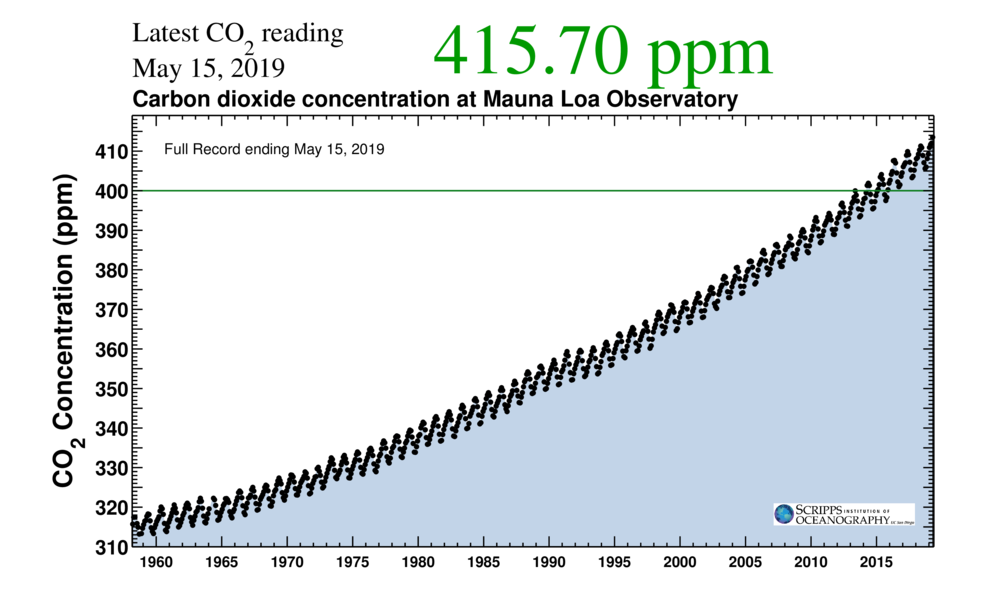
\includegraphics[scale = 0.3]{carbon.png}}
\end{center}
\begin{center}
\begin{tabular}{|c|c|c|c|c|c|c|}
\hline
Years passed since 1960 & 0 & 5 & 10 & 15 & 20 & 25 \\
\hline
$CO_2$ level (ppm) & 317 & 320 & 326 & 331 & 339 & 346 \\
\hline
Years passed since 1960 & 30 & 35 & 40 & 45 & 50 & 55\\
\hline
$CO_2$ level (ppm) & 354 & 361 & 370 & 380 & 390 & 401\\
\hline
\end{tabular}
\end{center}
(Data from: \href{ftp://aftp.cmdl.noaa.gov/products/trends/co2/co2_annmean_mlo.txt}{NOAA})
\end{Exercise}

\begin{Exercise}
Radioactive decay is modelled by $N = N_0e^{-kt}$, where $N_0$ and $k$ are the initial concentration and the decay constant respectively. While the expression is exponential, not linear, the technique of linear fit can still be applied if the data undergoes linearization. Show that by the substitution $n = \ln N$ the equation can be transformed into a linear equation $n = \ln N = \ln N_0 - kt = n_0 - kt$. Hence find the best linear fit on $(t, n)$ by finding the parameters $(n_0, k)$ from the experimental data on the radioactive isotope Sodium-24 below and recover the decay constant and initial mass.
\begin{center}
\begin{tabular}{|c|c|c|c|c|c|c|}
\hline
Time passed (hr) & 6 & 8 & 12 & 24 & 36 & 48\\
\hline
Mass (g) & 75.8 & 69.1 & 57.3 & 33.0 & 18.8 & 10.8\\
\hline
\end{tabular}
\end{center}
\end{Exercise}


\chapter{Discrete Fourier Transform}
We now discuss a powerful mathematical tool that can be approached from a least-square approximation view point. In last sections, we see how to fit a polynomial curve to some data. It is natural to ask, if there are any other types of curves that can be fitted to our interests. In the area of Earth Science, many phenomena can be described by the notion of waves, which are generally sinusoidal, e.g. atmospheric wave, seismic wave, electromagnetic wave. Hence, we may want to investigate if we can interpolate some data by using sines and cosines, and this is the central idea of what is known as Fourier Transform.

\section{Background and Types of Discrete Fourier Transform}
Fourier Transform and other related results are supported by the Fourier Theorem, which suggests that a function can be approximated by the sum of some sine-cosine series under some conditions. This implies that we can decompose a function into different sinusoidal waves, each having a certain amplitude, or called the Fourier coefficient. The resultant series has the name Fourier Series.
\begin{thm}
A periodic, smooth function $f(x)$ in the interval $[0,2\pi]$ can be approximated by the Fourier Series
\begin{align*}
S(f(x)) &= C_0 + A_1 \cos(x) + A_2 \cos(2x) + \cdots + B_1 \sin(x) + B_2 \sin(2x) + \cdots \\
&= C_0 + \sum_{k=1}^{\infty} (A_k \cos(kx) + B_k \sin(kx))
\end{align*}
\end{thm}
For a function that has an interval $[a,b]$ not exactly the same as $[0,2\pi]$, we can always scale it by replacing $x$ by the substitution $x' = 2\pi(\frac{x-a}{b-a})$. For non-periodic function over a fixed interval, we can extend it so that it behaves like a periodic one, by copying and pasting the same function over and over periodically.\\
\\
Here we provide a well-known example, the Fourier Series of $f(x) = x$ over $[0, 2\pi]$. We omit the calculation, and the answer is
\begin{align*}
S(x) &= \pi - 2 \sum_{k=1}^{\infty} \frac{\sin(kx)}{k} \\
&= \pi - 2 (\sin(x) + \frac{1}{2} \sin(2x) + \frac{1}{3} \sin(3x) + \cdots)
\end{align*}

\subsection{Discrete Fourier Transform, Real}
In Earth Science, and other fields like Engineering, often we are not given a function that has an analytical form to work with. Instead, we collect data from measurements at a fixed sampling rate, and what we obtain is a discrete time series. However, we can still apply the ideas of Fourier, and try to approximate and interpolate the finite time series with sinusoidal waves. Assume that, we have $n$ data points collected for the time series $f(t)$, evenly spaced at time $t = 0, 1, 2, \cdots, n-1$. We can scale the time range to $[0,2\pi]$ as what is suggested above, by making a change of variable $t' = 2\pi \frac{t}{n}$.\\
\\
Then, we can search a way to express the time series with sines and cosines of different frequencies like $\sin(t') = \sin((\frac{2\pi}{n})t), \sin(2t') = \sin((\frac{2\pi}{n})2t), \cdots$, and $\cos(t') = \cos((\frac{2\pi}{n})t), \cos(2t') = \cos((\frac{2\pi}{n})2t), \cdots$. The corresponding frequencies are $\frac{2\pi}{n}, 2(\frac{2\pi}{n}), \cdots$. In general, we propose an approximated form up to order $m$ as
\begin{align*}
S(f(t)) &= C_0 + A_1\cos((\frac{2\pi}{n})t) + A_2\cos((\frac{2\pi}{n})2t) + \cdots + A_m\cos((\frac{2\pi}{n})mt)\\
&\quad + B_1\sin((\frac{2\pi}{n})t) + B_2\sin((\frac{2\pi}{n})2t) + \cdots + B_m\sin((\frac{2\pi}{n})mt)\\
&= C_0 + \sum_{k=1}^{m} \left[A_k \cos((\frac{2\pi kt}{n})) + B_k \sin((\frac{2\pi kt}{n}))\right]
\end{align*}
Assume that we only use a few of sines and cosines for the approximation, such that the order $m$ much is less than the number of data points $n$, specifically, $2m+1 \leq n$. The least-square method is then set to find the best-fit parameters $C_0, A_1, B_1, \cdots, A_m, B_m$ for the system $G\vec{\beta} = \vec{d}$, where
\begin{align*}
G =
\begin{bmatrix}
1 & 1 & 0 & \cdots & 1 & 0 \\
1 & \cos(\frac{2\pi}{n}) & \sin(\frac{2\pi}{n}) & \cdots & \cos(\frac{2\pi m}{n}) & \sin(\frac{2\pi m}{n}) \\
1 & \cos(\frac{2\pi(2)}{n}) & \sin(\frac{2\pi(2)}{n}) & \cdots & \cos(\frac{2\pi (2m)}{n}) & \sin(\frac{2\pi (2m)}{n}) \\
\vdots & \vdots & \vdots & & \vdots & \vdots \\
1 & \cos(\frac{2\pi(n-1)}{n}) & \sin(\frac{2\pi(n-1)}{n}) & \cdots & \cos(\frac{2\pi (n-1)m}{n}) & \sin(\frac{2\pi (n-1)m}{n}) \\
\end{bmatrix}
\end{align*}
is a $n \times (2m+1)$ matrix and
\begin{align*}
&\vec{\beta} = 
\begin{bmatrix}
C_0 \\
A_1 \\
B_1 \\
\vdots \\
A_m \\
B_m
\end{bmatrix}
&\vec{d} = 
\begin{bmatrix}
f(0) \\
f(1) \\
f(2) \\
\vdots \\
f(n-1)
\end{bmatrix}
\end{align*}
are vectors with $2m+1$ and $n$ entries respectively. From theorem \ref{bestfit}, we know that the best parameters are found by
\begin{align*}
\vec{\beta_f} = (G^TG)^{-1}G^T\vec{d}
\end{align*}
However, we can greatly simplify the expression, by noticing that every column vector of sine/cosine is orthogonal to each other. If we write each sine-cosine term as a complex exponential using Euler's formula in definition \ref{Euler}, then each column vector of a sine-cosine pair in $G$ with a frequency of $2\pi k/n$, where both $k$ and $n$ are integers, can be expressed by the real and imaginary parts of
\begin{align*}
\left[\exp(\imath \frac{2\pi k}{n} t)\right]_{t = 0,1,2,\cdots,n-1}
&= \left[\cos(\frac{2\pi k}{n} t) + \imath\sin(\frac{2\pi k}{n} t) \right]_{t = 0,1,2,\cdots,n-1}
\end{align*}
or in the other way around,
\begin{align*}
\left[\exp(-\imath \frac{2\pi k}{n} t)\right]_{t = 0,1,2,\cdots,n-1}
&= \left[\cos(\frac{2\pi k}{n} t) - \imath\sin(\frac{2\pi k}{n} t) \right]_{t = 0,1,2,\cdots,n-1}
\end{align*}
We now first prove that the two column vectors of a sine-cosine pair that has the same frequency are orthogonal. We take the sum of squares of the first expression, which gives
\begin{align*}
\sum_{t=0}^{n-1} (\exp(\imath \frac{2\pi k}{n} t))^2 &= \sum_{t=0}^{n-1} (\cos(\frac{2\pi k}{n} t) + \imath\sin(\frac{2\pi k}{n} t))^2 \\
\sum_{t=0}^{n-1} \exp(\imath \frac{4\pi k}{n} t) &= \sum_{t=0}^{n-1} (\cos^2(\frac{2\pi k}{n} t) + 2\imath\sin(\frac{2\pi k}{n} t)\cos(\frac{2\pi k}{n} t) - \sin^2(\frac{2\pi k}{n} t))
\end{align*}
Notice that the left hand side is a geometric sequence with a common ratio $r = \exp(\imath 4\pi k/n)$, whose sum is seen to be
\begin{align*}
\frac{1-r^n}{1-r} &= \frac{1 - \exp(\imath 4\pi k)}{1 - \exp(\imath 4\pi k/n)} = 0
\end{align*}
as $\exp(\imath 4\pi k)$ is just $1$. By comparing the real and imaginary parts, we know that
\begin{align*}
\sum_{t=0}^{n-1} \cos^2(\frac{2\pi k}{n} t) &= \sum_{t=0}^{n-1} \sin^2(\frac{2\pi k}{n} t) \\
\sum_{t=0}^{n-1} \sin(\frac{2\pi k}{n} t)\cos(\frac{2\pi k}{n} t) &= 0
\end{align*}
The second equation shows that the two column vectors representing the sine and cosine wave of the same frequency have a dot product of zero and hence are orthogonal.\\
\\
Utilizing the complex formulations, we can also prove that column vectors of sine/cosine waves with different frequencies are orthogonal as well. Here we prove one of the cases, where the first wave is a sine a frequency of $2\pi k/n$, and the second wave is also a sine, of a frequency of $2\pi l/n$, where $k \neq l$ are both integers. We start by considering the sum of products between
\begin{align*}
\left[\exp(\imath \frac{2\pi k}{n} t)\right]_{t = 0,1,2,\cdots,n-1} = \left[\cos(\frac{2\pi k}{n} t) + \imath\sin(\frac{2\pi k}{n} t) \right]_{t = 0,1,2,\cdots,n-1}   
\end{align*}
and
\begin{align*}
\left[\exp(\imath \frac{2\pi l}{n} t)\right]_{t = 0,1,2,\cdots,n-1} = \left[\cos(\frac{2\pi l}{n} t) + \imath\sin(\frac{2\pi l}{n} t) \right]_{t = 0,1,2,\cdots,n-1}   
\end{align*}
The results are similar to the above analysis. Particularly,
\begin{align*}
\sum_{t=0}^{n-1} \cos(\frac{2\pi k}{n} t)\cos(\frac{2\pi l}{n} t) - \sum_{t=0}^{n-1} \sin(\frac{2\pi k}{n} t)\sin(\frac{2\pi l}{n} t) &= 0 
\end{align*}
We can also consider another dot product between $\left[\exp(\imath \frac{2\pi k}{n} t)\right]_{t = 0,1,2,\cdots,n-1}$ and
\begin{align*}
\left[\exp(-\imath \frac{2\pi l}{n} t)\right]_{t = 0,1,2,\cdots,n-1} = \left[\cos(\frac{2\pi l}{n} t) - \imath\sin(\frac{2\pi l}{n} t) \right]_{t = 0,1,2,\cdots,n-1}       
\end{align*}
This yields another relation as
\begin{align*}
\sum_{t=0}^{n-1} \cos(\frac{2\pi k}{n} t)\cos(\frac{2\pi l}{n} t) + \sum_{t=0}^{n-1} \sin(\frac{2\pi k}{n} t)\sin(\frac{2\pi l}{n} t) &= 0 
\end{align*}
From the two derived equations, we can conclude that
\begin{align*}
\sum_{t=0}^{n-1} \sin(\frac{2\pi k}{n} t)\sin(\frac{2\pi l}{n} t) &= 0    
\end{align*}
The orthogonality relations can be proven for sine vs cosine/cosine vs cosine of different frequencies as well. We will now establish the last result, the dot product of any cosine/sine column vector with a specific frequency $2\pi k/n$ with itself. We can consider the sum of products between
$\left[\exp(\imath \frac{2\pi k}{n} t)\right]_{t = 0,1,2,\cdots,n-1}$ and $\left[\exp(-\imath \frac{2\pi k}{n} t)\right]_{t = 0,1,2,\cdots,n-1}$. This time, the left hand side is not a geometric series, but rather $n$ terms of $1$. The relation is
\begin{align*}
\sum_{t=0}^{n-1} \cos^2(\frac{2\pi k}{n} t) + \sum_{t=0}^{n-1} \sin^2(\frac{2\pi k}{n} t) &= \sum_{t=0}^{n-1} \exp(\imath \frac{2\pi k}{n} t)\exp(-\imath \frac{2\pi k}{n} t) \\
&= \sum_{t=0}^{n-1} (1) \\
&= n
\end{align*}
Actually it roots from the fact that the sum of a sine-cosine square pair is $1$. Not long before, we have arrived at the equation
\begin{align*}
\sum_{t=0}^{n-1} \cos^2(\frac{2\pi k}{n} t) &= \sum_{t=0}^{n-1} \sin^2(\frac{2\pi k}{n} t)     
\end{align*}
Solving the two equations yields
\begin{align*}
\sum_{t=0}^{n-1} \cos^2(\frac{2\pi k}{n} t) &= \sum_{t=0}^{n-1} \sin^2(\frac{2\pi k}{n} t) = \frac{n}{2}    
\end{align*}
Hence the product $G^TG$, where each entry will be the dot products between vectors of sines and cosines, will be
\begin{align*}
G^TG =
\begin{bmatrix}
n & 0 & 0 & \cdots \\
0 & \frac{n}{2} & 0 & \\
0 & 0 & \frac{n}{2} & \\
\vdots & & & \ddots
\end{bmatrix}
\end{align*}
and
\begin{align*}
(G^TG)^{-1} = \frac{1}{n}
\begin{bmatrix}
1 & 0 & 0 & \cdots \\
0 & 2 & 0 & \\
0 & 0 & 2 & \\
\vdots & & & \ddots
\end{bmatrix}    
\end{align*}
So the best-fit parameters are
\begin{align*}
\vec{\beta_f} &= (G^TG)^{-1}G^T\vec{d} \\
\begin{bmatrix}
C_0 \\
A_1 \\
B_1 \\
\vdots \\
\end{bmatrix}
&= \frac{1}{n} 
\begin{bmatrix}
1 & 0 & 0 & \cdots \\
0 & 2 & 0 & \\
0 & 0 & 2 & \\
\vdots & & & \ddots
\end{bmatrix} 
\begin{bmatrix}
1 & 1 & 1 & \cdots \\
1 & \cos(\frac{2\pi}{n}) & \cos(\frac{2\pi(2)}{n}) & \\
0 & \sin(\frac{2\pi}{n}) & \sin(\frac{2\pi(2)}{n}) &  \\
\vdots & & & \ddots
\end{bmatrix}
\begin{bmatrix}
f(0)\\
f(1)\\
f(2)\\
\vdots
\end{bmatrix} \\
\begin{bmatrix}
C_0 \\
A_1 \\
B_1 \\
\vdots \\
\end{bmatrix}
&= 
\frac{1}{n}
\begin{bmatrix}
1 & 1 & 1 & \cdots \\
2 & 2\cos(\frac{2\pi}{n}) & 2\cos(\frac{2\pi(2)}{n}) & \\
0 & 2\sin(\frac{2\pi}{n}) & 2\sin(\frac{2\pi(2)}{n}) &  \\
\vdots & & & \ddots
\end{bmatrix}
\begin{bmatrix}
f(0)\\
f(1)\\
f(2)\\
\vdots
\end{bmatrix} 
\end{align*}
Detailed expressions are
\begin{align*}
C_0 &= \frac{1}{n}(f(0) + f(1) + f(2) + \cdots + f(n-1)) \\
&= \frac{1}{n}\sum_{t=0}^{n-1} f(t) \\
A_m &= \frac{2}{n}(f(0) + f(1)\cos(\frac{2\pi m}{n}) + \cdots + f(n-1)\cos(\frac{2\pi (n-1)m}{n})) \\
&= \frac{2}{n}\sum_{t=0}^{n-1} f(t)\cos(\frac{2\pi mt}{n}) \\
B_m &= \frac{2}{n}(f(1)\sin(\frac{2\pi m}{n}) + \cdots + f(n-1)\sin(\frac{2\pi (n-1)m}{n})) \\
&= \frac{2}{n}\sum_{t=0}^{n-1} f(t)\sin(\frac{2\pi mt}{n})
\end{align*}

\begin{exmp}
\label{ex11.2.1}
Fit the following time-series with sinusoidal waves up to order $m=1$. $f(0) = 1, f(1) = 4, f(2) = 6, f(3) = 3, f(4) = 5$.\\
\\
The order $m=1$ means that there are only three constituents, which are the constant term, and a sine-cosine pair with a frequency of $\frac{2\pi k}{n}$ where $k=1$, $n=5$. The best-fit parameters will be
\begin{align*}
\begin{bmatrix}
C_0 \\
A_1 \\
B_1
\end{bmatrix}
&= 
\frac{1}{5}
\begin{bmatrix}
1 & 1 & 1 & 1 & 1 \\
2 & 2\cos(\frac{2\pi}{5}) & 2\cos(\frac{2\pi(2)}{5}) & 2\cos(\frac{2\pi(3)}{5}) & 2\cos(\frac{2\pi(4)}{5}) \\
0 & 2\sin(\frac{2\pi}{5}) & 2\sin(\frac{2\pi(2)}{5}) & 2\sin(\frac{2\pi(3)}{5}) & 2\sin(\frac{2\pi(4)}{5})
\end{bmatrix}
\begin{bmatrix}
f(0)\\
f(1)\\
f(2)\\
f(3)\\
f(4)
\end{bmatrix} 
\end{align*}
\begin{align*}
C_0 &= \frac{1}{5} (1+4+6+3+5) = \frac{19}{5} \\
A_1 &= \frac{2}{5} (1 + 4\cos(\frac{2\pi}{5}) + 6\cos(\frac{2\pi(2)}{5}) + 3\cos(\frac{2\pi(3)}{5}) + 5\cos(\frac{2\pi(4)}{5})) \\
&= -\frac{7}{5} \\
B_1 &= \frac{2}{5} (4\sin(\frac{2\pi}{5}) + 6\sin(\frac{2\pi(2)}{5}) + 3\sin(\frac{2\pi(3)}{5}) + 5\sin(\frac{2\pi(4)}{5})) \\
&\approx 0.325
\end{align*}
So the best sinusoidal fit of order $m=1$ for the time-series concerned is
\begin{align*}
f(t) = \frac{19}{5} - \frac{7}{5} \cos(\frac{2\pi}{5}t) + 0.325 \sin(\frac{2\pi}{5}t)
\end{align*}
Short Exercise: Find an improved approximation with order $m = 2$.
\end{exmp}

However, there are two problems with the formulation. First, since we may want to make the approximation as good as possible, we have to know how high the order $m$ needs to be. Let's continue with the assumption that the time step is $1$, so that the sampling points are at $t = 0, 1, 2, \cdots, n-1$. Then the Nyquist Sampling Theorem tells us that there is a cap for $m$.
\begin{thm}
For a evenly spaced time-series that has a time step of $1$, any wave with a linear frequency $f > f_{ny} = 1/2$ or angular freqency $\omega > \omega_{ny} = \pi$ cannot be detected. More generally, for a time step of $\Delta t$, the Nyquist frequnecy is $\omega_{ny} = \frac{\pi}{\Delta t}$.
\end{thm}
So it means that we only need the sines/cosines up to the order $m_c$, where $m_c$ is inferred by looking at the expression of angular frequency inside the expression of sines/cosines, that is
\begin{align*}
\frac{2\pi m}{n} \leq \frac{2\pi m_c}{n} &= \pi \\
m \leq m_c &= \frac{n}{2}
\end{align*}
\paragraph{Proof} We illustrate a portion of the theorem by proving
\begin{align*}
\cos(\frac{2\pi (m_c + (m_c - m))}{n}) &= \cos(\frac{2\pi (m_c - (m_c - m))}{n}) \\
&= \cos(\frac{2\pi m}{n})
\end{align*}
so that mirroring $m$ about $m_c$ has no effect on the cosine wave. But the left hand side is simply
\begin{align*}
\cos(\frac{2\pi (m_c + (m_c - m))}{n}) &= \cos(\frac{4\pi mc}{n} - \frac{2\pi m}{n}) \\
&= \cos(\frac{4\pi (n/2)}{n} - \frac{2\pi m}{n}) \\
&= \cos(2\pi - \frac{2\pi m}{n}) \\
&= \cos(\frac{2\pi m}{n})
\end{align*}

For $n$ is even, then we have frequencies from zero to $m_c = n/2$. Notice that the zero frequency constant term contributes a single parameter, every other frequencies contribute two parameters as sines/cosines, and the maximum frequency $m_c = n/2$ only contributes one parameter of cosine (the corresponding diagonal entry for $(G^TG)^{-1}$ will be $1/n$ instead of $2/n$), as the sine function will be always zero at that frequency. This means that there are $n$ parameters as total.\\
\\
For $n$ is odd, the situation is the same except at the maximum frequency $m_c = (n-1)/2$ which contributes two parameters as a sine-cosine pair. Counting also reveals that the amount of parameters is also $n$. In both cases, there can be at most $n$ sinusoidal curves for fitting $n$ data points. Since the amount of parameters is the same as the number of data, it becomes an interpolation that passes through all the given data points, and this forms the foundation of Discrete Fourier Transform. But the difference between odd/even $n$ has to be remembered when we are tackling the maximum frequency signal. \\
\\
Another drawback of the approach is that it uses sine-cosine pairs for computation. In \autoref{section:complexno}, we have learnt the power of complex exponentials to simultaneously represent sines and cosines. Therefore, one may explore the possibility of using complex exponentials to do Discrete Fourier Transform. This has the benefits of simplicity and also convenience when programming.

\subsection{Discrete Fourier Transform, Complex}

Now extending the ideas from the last section, we propose an interpolation scheme which uses $\exp(\imath\frac{2\pi k}{n}t)$, for a time-series with $n$ data, evenly spaced by a time step of $1$. The range of $k$ will be from $-\frac{n}{2}, -(\frac{n}{2}-1), \cdots, 0, \frac{n}{2}-1$ for even $n$ and $-\frac{n-1}{2}, -(\frac{n-1}{2}-1), \cdots, 0, \frac{n-1}{2}$ for odd $n$. Both ranges ensure that the total number of sinusoidal waves used is exactly $n$.\\
\\
Each pair of $k$ and $-k$, or $\exp(\imath\frac{2\pi k}{n}t)$, and $\exp(-\imath\frac{2\pi k}{n}t)$ in combination, gives rise to $\cos(\frac{2\pi k}{n}t)$ and $\sin(\frac{2\pi k}{n}t)$ by properties \ref{sincoscomplex}, and so we see the correspondence between the real and complex version of Discrete Fourier Transform.\\
\\
Now, the matrix $G$ has the form of
\begin{align*}
G =
\begin{bmatrix}
1 & 1 & \cdots & 1 & 1 & \cdots\\
1 & \exp(\imath\frac{2\pi}{n}) & \cdots & \exp(\imath\frac{2\pi(n/2-1)}{n}) & \exp(\imath\frac{2\pi(-n/2)}{n}) & \cdots \\
1 & \exp(\imath\frac{2\pi(2)}{n}) & \cdots & \exp(\imath\frac{2\pi(n/2-1)(2)}{n}) & \exp(\imath\frac{2\pi(-n/2)(2)}{n}) & \cdots\\
\vdots & \vdots & & \vdots & \vdots & \\
1 & \exp(\imath\frac{2\pi(n-1)}{n}) & \cdots & \exp(\imath\frac{2\pi(n/2-1)(n-1)}{n}) & \exp(\imath\frac{2\pi(-n/2)(n-1)}{n}) & \cdots
\end{bmatrix}
\end{align*}
for even $n$, where each column representing frequencies that have $k = 0, 1, \cdots, \frac{n}{2}-1$, $-\frac{n}{2}, \cdots, -1$. This is a common convention where we starts from $k = 0$, and increases to the largest positive $k$, then flips the sign and resumes from the largest negative $k$, goes all the way back to $k = -1$. Odd $n$ has a similar form of $G$, but with all the $k$ replaced by the appropriate integer range.\\
\\
Notice that as we are now working with complex matrices, the normal equation is modified and the formula of the best-fit parameters are now $\vec{\beta}_f = (G^*G)^{-1}G^*\vec{d}$, contrary to theorem \ref{bestfit} as the transpose is replaced by conjugate transpose/Hermitian. The entries of $G^*G$ are the complex dot products between the column vectors of $G$.\\
\\
The orthogonality relation between different column vectors of complex exponentials is very easy to find. The procedure is similar to what we have done when proving the orthogonality for the real case, but even less tedious. The key point is to write the complex dot product along the two columns as a geometric sequence, that when the values of $k$ are different, will be evaluated to zero. The readers are invited to verify this result, as well as the fact that the complex dot product between any column vector of complex exponentials and itself is $n$. Thus, the expression $G^*G$ is just $nI$, and $(G^*G)^{-1} = \frac{1}{n} I$.\\
\\
Now we denote the best-fit parameters, or coefficients by $C_k$. Subsequently,
\begin{align*}
\vec{\beta}_f &= (G^*G)^{-1}G^*\vec{d} \\
&= \frac{1}{n}G^*\vec{d} \\
\begin{bmatrix}
C_0 \\
C_1 \\
\vdots \\
C_{n/2-1} \\
C_{-n/2} \\
\vdots
\end{bmatrix}
&= 
\frac{1}{n}
\begin{bmatrix}
1 & 1 & 1 & \cdots \\
1 & \exp(-\imath\frac{2\pi}{n}) & \exp(-\imath\frac{2\pi(2)}{n}) & \cdots \\
\vdots & \vdots & \vdots & \\
1 & \exp(-\imath\frac{2\pi(n/2-1)}{n}) & \exp(-\imath\frac{2\pi(n/2-1)(2)}{n}) & \cdots \\
1 & \exp(-\imath\frac{2\pi(-n/2)}{n}) & \exp(-\imath\frac{2\pi(-n/2)(2)}{n}) & \cdots 
\end{bmatrix}
\begin{bmatrix}
f(0) \\
f(1) \\
f(2) \\
\vdots
\end{bmatrix}
\end{align*}
Again this is for even $n$, we ought to replace the coefficients and complex exponentials appropriately for odd $n$. We now conclude the method of Complex Discrete Fourier Transform in a compact way as follows.
\begin{defn}
The coefficients, or amplitudes, of the Discrete Fourier Transform in complex form are
\begin{align*}
C_k = \sum_{t=0}^{n-1} f(t)\exp(-\imath\frac{2\pi k}{n}t)
\end{align*}
where $n$ is the number of data. $k$ are all integers ranging from $[-\frac{n}{2}, \frac{n}{2}-1]$ for even $n$, and $[-\frac{n-1}{2}, \frac{n-1}{2}]$ for odd $n$. The negative sign in the complex exponentials comes from the conjugate transpose in the formulation. In the most common convention the factor $1/n$ is removed. For a time step $\Delta t$ different from $1$, the expression is
\begin{align*}
C_k = \sum_{t=0}^{n-1} f(t)\exp(-\imath\frac{2\pi k}{n\Delta t}t)
\end{align*}
We will denote the series of $C_k$ by $F(k)$ or $\hat{f}(k)$.
\end{defn}
The relation between $C_k$ and the parameters $A_k$, $B_k$ in the real counterpart are inferred from properties \ref{sincoscomplex} and comparing the expression for the real case, that is
\begin{align*}
A_k &= \frac{C_k + C_{-k}}{n} \\
B_k &= -\frac{(C_k - C_{-k})}{n\imath}
\end{align*}
for $k \neq 0$. A closer inspection reveals that, since sine is an odd function, and cosine is an even function, $\Re(C_k) = \Re(C_{-k})$, and $\Im(C_k) = -\Im(C_{-k})$, or in other words, $C_k$ and $C_{-k}$ are a pair of complex conjugate. And so the relation between the real and complex Discrete Fourier Transform is
\begin{proper}
\label{FTrealcomplex}
The amplitudes $A_k$, $B_k$ in real Discrete Fourier Transform, and $C_k$ in complex Discrete Fourier Transform satisfy
\begin{align*}
A_k &= 2\Re(C_k)/n \\
B_k &= -2\Im(C_k)/n
\end{align*}
\end{proper}

\begin{exmp}
Find the Complex Discrete Fourier Transform for the time-series in example \ref{ex11.2.1}.\\
\\
Using the formula above, we have
\begin{align*}
C_0 &= 1+4+6+3+5 = 19 \\
C_1 &= 1 + 4\exp(-\imath\frac{2\pi}{5}) + 6\exp(-\imath\frac{2\pi(2)}{5}) + 3\exp(-\imath\frac{2\pi(3)}{5}) + 5\exp(-\imath\frac{2\pi(4)}{5}) \\
&= -3.5 - 0.812\imath \\
C_2 &= 1 + 4\exp(-\imath\frac{2\pi(2)}{5}) + 6\exp(-\imath\frac{2\pi(2)(2)}{5}) \\
&\quad+ 3\exp(-\imath\frac{2\pi(2)(3)}{5}) + 5\exp(-\imath\frac{2\pi(2)(4)}{5}) = -3.5 + 3.441 \imath
\end{align*}
$C_{-1}$ and $C_{-2}$ are complex conjugates of $C_1$ and $C_2$ respectively. \\
Short Exercise: Check if properties \ref{FTrealcomplex} is true in this example.
\end{exmp}

We can also undo the Discrete Fourier Transform and recover the initial time-series by its inverse, defined as follows.
\begin{defn}
The inverse Discrete Fourier Transform is done by
\begin{align*}
f(t) &= \frac{1}{n}\sum_{k=0}^{n-1} F(k)\exp(\imath\frac{2\pi k}{n}t)
\end{align*}
Sometimes we use the symbol $F^{-1}$ to denote the inverse operation.
\end{defn}

\section{Convolution}
Convolution is often used in the world of Fourier Transform due to a beautiful theorem that will be introduced later. In the area of Earth Science, as well as Physics and Statistics, convolution also has a place, for describing phenomena, or their solutions. Now we will introduce how convolution in a discrete sense is defined first, and a daily example will be provided as an illustration.\\
\\
Discrete Convolutions always involved two time-series as below.
\begin{defn}
The convolution $h(t)$ between two discrete time-series $f(t)$ and $g(t)$ is written $f(t) * g(t)$, defined as
\begin{align*}
h(t) = f(t) * g(t) = \sum_{\tau=-\infty}^{\infty} f(\tau) g(t-\tau)
\end{align*}
if $\tau$ takes a value so that the index in either $f$ or $g$ is out of the range, then the term becomes zero.
\end{defn}
For instance, if $f(t)$ is defined from $t = 0$ and $t = 4$ and $g(t)$ is defined from $t = 0$ and $t = 6$, then
\begin{align*}
h(0) &= f(0)g(0) \\
h(1) &= f(0)g(1-0) + f(1)g(1-1) = f(0)g(1) + f(1)g(0) \\
h(4) &= f(0)g(4-0) + f(1)g(4-1) + f(2)g(4-2) + f(3)g(4-3) + f(4)g(4-4) \\
&= f(0)g(4) + f(1)g(3) + f(2)g(2) + f(3)g(1) + f(4)g(0)
\end{align*}
and
\begin{align*}
h(6) &= f(0)g(6) + f(1)g(5) + f(2)g(4) + f(3)g(3) + f(4)g(2) \\
h(9) &= f(3)g(6) + f(4)g(5) \\
h(10) &= f(4)g(6)
\end{align*}
It can be deduced that the resulted convolution will has a length of $m + n - 1$ if the two input time-series have a length of $m$ and $n$.

\begin{exmp}
The probability of Mary getting married within some years can be described by the time-series $q(t)$, where
\begin{align*}
q(t) = 
\begin{cases}
0.2 & 0 \leq t \leq 2 \\
0.1 & 3 \leq t \leq 6 \\
0 & t \geq 7
\end{cases}
\end{align*}
The probability $r(t)$ that Mary gives birth to a baby some years $t$ after marriage is
\begin{align*}
r(t) = 
\begin{cases}
0 & t = 0 \\
0.15 & 1 \leq t \leq 4 \\
0.08 & 5 \leq t \leq 9 \\
0 & t \geq 10
\end{cases}    
\end{align*}
Find the net probability of Mary getting a baby at some years $t$ from now on, assuming she will only get pregnant after married. \\
\\
We identify the required probability $p(t) = q(t) * r(t)$ is a convolution between $q(t)$ and $r(t)$, which effectively have a length of $7$ and $9$. Particularly, taking $t = 5$ as an example, then we have
\begin{align*}
p(t = 5) &= P(\text{Birth 5 years later}|\text{Married now})P(\text{Married now}) \\
&\quad+ P(\text{Birth 4 years later}|\text{Married 1 year later})P(\text{Married 1 year later})\\
&\quad+ \cdots \\
&\quad+ P(\text{Birth 1 year later}|\text{Married 4 years later})P(\text{Married 4 years later}) \\
&= q(0)r(5) + q(1)r(4) + q(2)r(3) + q(3)r(2) + q(4)r(1) \\
&= (0.2)(0.08) + (0.2)(0.15) + (0.2)(0.15) + (0.1)(0.15) + (0.1)(0.15) \\
&= 0.106
\end{align*}
where $P(A|B)$ is the probability of getting $A$ when $B$ happens.\\
Short Exercise: Find the chance of Mary getting a baby at $8$ years later by convolution.
\end{exmp}

If, the two discrete time-series are infinitely long, then we have the following weaker version of Convolution Theorem for discrete Fourier Transform.
\begin{thm}
For two infinitely long discrete time-series $f(t)$ and $g(t)$, we have
\begin{align*}
F[f(t) * g(t)](k) &= \hat{f}(k)\hat{g}(k)
\end{align*}
The Discrete Fourier Transform of the convolution between the two time-series is equal to the product of the two Discrete Fourier Transforms for their own.
\end{thm}
It is worth emphasized again that this is a much weaker statement compared to the full form, which is known as the Circular Convolution Theorem, that do the convolution for two finite time-series in a cyclic manner, and works in two directions.

\section{Exercise}
\begin{Exercise}
Carry out Discrete Fourier Transform for the following data.
\begin{center}
\begin{tabular}{|c|c|c|c|c|c|c|}
\hline
unit time & 0 & 1 & 2 & 3 & 4 \\
\hline
f(t) & 4 & 6 & 7 & 1 & 3  \\
\hline
unit time & 5 & 6 & 7 & 8 & 9 \\
\hline
f(t) & 2 & 3 & 5 & 2 & 6\\
\hline
\end{tabular}
\end{center}
Find the amplitude and phase of the sinusoidal wave corresponding to an angular frequency of $2\pi\frac{3}{10}$. 
\end{Exercise}

\begin{Exercise}
Download an \href{https://cds.climate.copernicus.eu/cdsapp#!/dataset/reanalysis-era5-single-levels?tab=overview}{ERA5 Temperature Dataset} over any time period of $5$ years. Select a location as you like, and extract the temperature time-series there. Apply Discrete Fourier Transform on the time series, and identify any dominant frequency or time period whose amplitude (the magnitude of complex coefficient) is large. Explain the peaks with Earth Science knowledge.
\end{Exercise}

\begin{Exercise}
Perform Fourier Transform on the time-series of the first Principal Direction in exercise (10.5).
\end{Exercise}
\chapter{Numerical Integration}

Sometimes, the integral of a function may have an analytical solution. However, for more complicated functions, closed-form solution is often unavailable or very difficult to obtain. In Earth Science or other Science fields, integrals that are hard to evaluate are not rare. The most common example is the integral of a Gaussian function
\begin{align*}
\int_{-\infty}^{t} e^{-\tau^2/(2\sigma^2)} d\tau
\end{align*}
that frequently appears as the cumulative distribution function of Normal Distribution. Sometimes we also need to calculate an integral from limited measurements. This forces us to apply \textit{Numerical Integration} methods to do the integration in a discrete manner. In the age of computers, this approach is feasible in many cases, as it can usually give an accurate estimate on the actual value of the integral.\\
\\
While integration methods themselves are not directly related to linear algebra, vectors and matrices provide a compact description to some of them, Therefore, they are worth to be mentioned, accounting for their importance in Earth Science.

\section{One-dimensional Numerical Integration}
We start from the simplest case, numerical integration for single integrals.

\subsection{Trapezoidal Rule}
The most straight-forward method is to go back to the definition of integral itself. Since integral can be regarded to be the sum of infinitely many small rectangles, we can approximate any integral by partitioning the area into some finite amount of rectangles, hoping the accuracy is not too bad. This method has the name \textit{Rectangle Rule}.\\
\\
We will not talk about the Rectangle Rule in details. Instead, we jump to an improved version which is a natural generalization of the Rectangle Rule. Often while using Rectangle Rule, we craft the rectangle with a height that is either the value of the function at the left (or right) interval. So, the approximation by rectangles will introduce substantial errors due to the difference between their heights and the right (left) intervals. We naturally amend this by using a trapezoid that touches the function at both intervals. This is called the \textit{Trapezoidal Rule}.\\
\begin{defn}
\label{1301}
The Trapezoidal Rule approximates an integral by
\begin{align*}
\int_a^b f(x) dx \approx \sum_{k=0}^{n-1} \frac{h}{2} (f(x_k) + f(x_{k+1}))  
\end{align*}
where we partition the interval $[a,b]$ into $n$ intervals evenly at $x_0, x_1, \cdots, x_n$ with a width of $h$. Expanding the summation gives
\begin{align*}
&\quad \sum_{k=0}^{n-1} \frac{h}{2} (f(x_k) + f(x_{k+1})) \\
&= \frac{h}{2} (f(x_0) + 2f(x_1) + 2f(x_2) + \cdots + 2f(x_{n-2}) + 2f(x_{n-1}) + f(x_n))
\end{align*}
\end{defn}

\begin{exmp}
Integrate $\cos(0.7\pi x)$ numerically by Trapezoidal Rule over $x = [0,2]$.\\
\\
We divide the interval into $5$ sub-intervals with a spacing of $h = 0.4$, $x_0 = 0, x_1 = 0.4, x_2 = 0.8, \cdots, x_5 = 2$. By definition \ref{1301}, we obtain an estimate of
\begin{align*}
&\quad \int_0^2 \cos(0.7\pi x) dx \\
&\approx \frac{0.4}{2} [\cos(0.7\pi (0)) + 2\cos(0.7\pi (0.4)) + 2\cos(0.7\pi (0.8))\\
&\quad + 2\cos(0.7\pi (1.2)) + 2\cos(0.7\pi (1.6)) + \cos(0.7\pi (2))] \\
&\approx -0.404
\end{align*}
The exact value is around $-0.432$.
\end{exmp}

\subsection{Simpson's Rule}
An even more powerful numerical integration method is to used quadratic curves to approximate the area under the curve. Different from Trapezoidal Rule, each quadratic curve used span two sub-intervals, so the total number of sub-intervals must be even. (If it is odd, then we can use Trapezoidal Rule for the last sub-interval.) This is known as the \textit{Simpson's Rule}.
\begin{defn}
\label{1302}
The Simpson's Rule approximates an integral by
\begin{align*}
\int_a^b f(x) dx \approx \sum_{l=0}^{m-1} \frac{2h}{6} (f(x_{2l}) + 4f(x_{2l+1}) + f(x_{2l+2}))  
\end{align*}
assuming the number of sub-interval over $[a,b]$ is even, $n = 2m$. Again each of them has a even spacing of $h$. Alternatively, we have
\begin{align*}
&\quad \sum_{l=0}^{m-1} \frac{2h}{6} (f(x_{2l}) + 4f(x_{2l+1}) + f(x_{2l+2})) \\
&= \frac{2h}{6} (f(x_0) + 4f(x_1) + 2f(x_2) + 4f(x_3) + \cdots + 2f(x_{n-2}) + 4f(x_{n-1}) + f(x_n))
\end{align*}
\end{defn}

\begin{exmp}
Integrate $f(x) = e^{-x}$ between $[0,1]$ using Simpson's Rule.\\
\\
We demonstrate by dividing the interval into $10$ sub-intervals with a width of $h=0.1$ and there are $5$ quadratic curves used for the estimation. From the $(1, 4, 2, 4, 1)$ pattern in definition \ref{1302}, we have
\begin{align*}
&\quad \int_0^1 e^{-x} dx \\
&\approx \frac{2(0.1)}{6}(e^0 + 4e^{-0.1} + 2e^{-0.2} + 4e^{-0.3} + 2e^{-0.4} \\
&\quad + 4e^{-0.5} + 2e^{-0.6} + 4e^{-0.7} + 2e^{-0.8} + 4e^{-0.9} + e^{-1}) \\
&\approx 0.63212
\end{align*}
The answer is very close to the exact value, with the first difference occurs at the $7$-th decimal place.\\ 
Short Exercise: Repeat the approximation with Trapezoidal Rule.
\end{exmp}

\section{Generalization and Discussion}
\subsection{Multi-dimensional Numerical Integration}
It can be inferred from the previous example that the two numerical integration methods above can be written in the form of dot product for single integrals. For Trapezoidal Rule, it is 
\begin{align*}
\frac{h}{2}
\begin{bmatrix}
f(x_0) & f(x_1) & f(x_2) & \cdots & f(x_{n-1}) & f(x_n)
\end{bmatrix}
\begin{bmatrix}
1 \\
2 \\
2 \\
\vdots \\
2 \\
1
\end{bmatrix}
\end{align*}
While for Simpson's Rule, it is
\begin{align*}
\frac{2h}{6}
\begin{bmatrix}
f(x_0) & f(x_1) & f(x_2) & f(x_3) & f(x_4) & \cdots & f(x_{n-2}) & f(x_{n-1}) & f(x_n)
\end{bmatrix}
\begin{bmatrix}
1 \\
4 \\
2 \\
4 \\
2 \\
\vdots \\
2 \\
4 \\
1
\end{bmatrix}
\end{align*}
Generalizing for the double integral of a function $f(x,y)$, the expression becomes a quadratic form. the Trapezoidal Rule has a form of
\begin{align*}
(\frac{h_x}{2})(\frac{h_y}{2})
\begin{bmatrix}
1 & 2 & 2 & \cdots & 1
\end{bmatrix}
\begin{bmatrix}
f(x_0,y_0) & f(x_1, y_0) & f(x_2, y_0) & \cdots & f(x_n, y_0) \\
f(x_0,y_1) & f(x_1, y_1) & f(x_2, y_1) & \cdots & \\
f(x_0,y_2) & f(x_1, y_2) & f(x_2, y_2) & \cdots & \\
\vdots & & & \ddots & \\
f(x_0,y_m) & & & & f(x_n,y_m)
\end{bmatrix}
\begin{bmatrix}
1 \\
2 \\
2 \\
\vdots \\
1
\end{bmatrix}   
\end{align*}
where $m$ and $n$ are the amounts of sub-intervals along $y$ and $x$-directions. Simpson's Rule for double integrals reads
\begin{align*}
(\frac{2h_x}{6})(\frac{2h_y}{6})
\begin{bmatrix}
1 & 4 & 2 & \cdots & 1
\end{bmatrix}
\begin{bmatrix}
f(x_0,y_0) & f(x_1, y_0) & f(x_2, y_0) & \cdots & f(x_n, y_0) \\
f(x_0,y_1) & f(x_1, y_1) & f(x_2, y_1) & \cdots & \\
f(x_0,y_2) & f(x_1, y_2) & f(x_2, y_2) & \cdots & \\
\vdots & & & \ddots & \\
f(x_0,y_m) & & & & f(x_n,y_m)
\end{bmatrix}
\begin{bmatrix}
1 \\
4 \\
2 \\
\vdots \\
1
\end{bmatrix}   
\end{align*}
assuming the step width $h_x$ and $h_y$ along the $x$ and $y$-direction. This is effectively equivalent to first apply the method in $x$/$y$-direction and then apply it again in $y$/$x$-direction.

\begin{exmp}
Numerically integrate the double integral $\int_1^4 \int_0^3 e^{-x}\cos(y) dxdy$ over the rectangular region $0 \leq x \leq 3$, $1 \leq y \leq 4$.\\
\\
We employ the Trapezoidal Rule with a step size of $h = 1$ along both $x$ and $y$-directions. From the formula above, we know that the approximation is given by
\begin{align*}
(\frac{1}{2})^2
\begin{bmatrix}
1 & 2 & 2 & 1
\end{bmatrix}
\begin{bmatrix}
e^{-0}\cos(1) & e^{-1}\cos(1) & e^{-2}\cos(1) & e^{-3}\cos(1) \\
e^{-0}\cos(2) & e^{-1}\cos(2) & e^{-2}\cos(2) & e^{-3}\cos(2) \\
e^{-0}\cos(3) & e^{-1}\cos(3) & e^{-2}\cos(3) & e^{-3}\cos(3) \\
e^{-0}\cos(4) & e^{-1}\cos(4) & e^{-2}\cos(4) & e^{-3}\cos(4) 
\end{bmatrix}
\begin{bmatrix}
1 \\
2 \\
2 \\
1
\end{bmatrix}       
\end{align*}
\end{exmp}
The value of this quadratic form is $-1.5039$, compared to the exact value of $-1.5187$.\\
Short Exercise: Use two-dimensional Simpson's Rule to compute this double integral again.\\
\\
The ideas for extending these two rules for triple integrals are similar. The integration methods are applied in the three directions, one after another. The formula can be expressed using tensors, which will be taught in the last chapter.

\subsection{Error Estimates}
Errors of Trapezoidal Rule is proportional to the square of step size, while Simpson’s Rule has an error proportional to the fourth power of step size. In general, Simpson’s Rule is more accurate. Below listed the detailed error estimates for these two methods in one-dimensional cases.
\begin{proper}
Given a definite, single integral of a function $f(x)$ to be numerically integrated over the region $[a,b]$, the maximum error incurred by Trapezoidal Rule is
\begin{align*}
\abs{E_T} \leq \frac{Q_2(b-a)}{12}h^2
\end{align*}
where $h$ is the step size, $Q_2$ is the absolute value of the maximum second derivative of the function, $\abs{f''(x)}$, in the range. Error of Simpson's Rule is bounded by
\begin{align*}
\abs{E_S} \leq \frac{Q_4(b-a)}{180}h^4
\end{align*}
$Q_4$ is similarly the absolute value of the maximum fourth derivative of the function, $\abs{f^{(4)}(x)}$.
\end{proper}
The actual error is usually much smaller than the theoretical bound. As a final note, Trapezoidal Rule and Simpson’s Rule belong to a wider class of integration formula called \textit{Newton-Cotes Quadrature Rule}.

\section{Exercise}

\begin{Exercise}
Use Trapezoidal Rule and Simpson's Rule to numerically integrate $\int_0^{8} \exp(-\frac{x^2}{8^2}) dx$. The spacing between each sampling point should be less than $1$. It is given that the value of the integral is about $5.97459306$, estimate the percentage errors of these two numerical integration methods.
\end{Exercise}

\begin{Exercise}
Use Trapezoidal Rule and Simpson's Rule to numerically integrate $\int_2^{10}\int_2^{10} \ln(x)\sqrt{y} dxdy$. The spacing between each grid point should be less than $1$.
\end{Exercise}

\begin{Exercise}
What is the error of Simpson's Rule if we integrate $f(x) = x^3 + 2x^2 + 3x + 4$ between $[0, 10]$?
\end{Exercise}
\chapter{Markov Chain}

In Earth Science, we often look at the time evolution of some variables, like temperature, rainfall etc. Sometimes, the variables can be modelled as random variables. A simple daily example will be tossing a coin (no matter it is fair or not), where the outcomes (head/tail) are probabilistic. Some Earth System examples are the chances of extreme weathers, or some slow geological processes. Such processes involving random variables are known as \textit{Stochastic Processes}, and we will visit the related Statistical concepts. Particularly, we will investigate the so-called \textit{Markov Chain}, which assumes the present state of a stochastic process only depends on the past. Modelling a stochastic process with Markov Chain can give more satisfactory results when it is believed that the process inherently correlates strongly with previous states, or is said to be have \textit{memory}.

\section{Basic Statistical Ideas for Markov Chain}

\subsection{Lagged Auto-correlation}

First, let's talk about how we determine if a time-series possesses some sorts of memory. Memory causes the past of a time-series to influence the present, and hence will leave a mark when we try to correlate the past and the present of the time-series. Here comes the idea of \textit{Lagged Auto-correlation}, which is the correlation between a time-series and itself, but one of them is lagged and shifted by a certain amount of days, $k$ (The direction of shifting does not matter much, and we only care about the overlapping part), and it is more specifically known as the \textit{Lag-k Auto-correlation}.

\begin{defn}
\label{1403}
The lag-k auto-correlation $r_k$ of a time-series $\{x\}$ is defined as
\begin{align*}
r_k &= \frac{\sum_{i=1}^{n-k}(x_i - \bar{x}_{-})(x_{i+k} - \bar{x}_{+})}{\sqrt{(\sum_{i=1}^{n-k}(x_i - \bar{x}_{-})^2) (\sum_{i=k+1}^{n}(x_i - \bar{x}_{+})^2)}}
\end{align*}
where $\{x_{-}\}$ and $\{x_{+}\}$ denotes the sequence representing the earliest and latest $n-k$ data. An overline denotes an average. Alternatively, the formula can be written as
\begin{align*}
r_k &= \frac{\text{Cov}(\{x_{-}\},\{x_{+}\})}{\sqrt{\text{Var}(\{x_{-}\}) \text{Var}(\{x_{+}\})}} \\
&= \frac{\text{Cov}(\{x_{-}\},\{x_{+}\})}{\sqrt{\text{Cov}(\{x_{-}\}, \{x_{-}\}) \text{Cov}(\{x_{+}\}, \{x_{+}\})}}
\end{align*}
where the definitions of variance and covariance are those from definitions \ref{variance} and \ref{covariance}.
\end{defn}
If the lag-k auto-correlation of a time-series is close to $1$ or $-1$, it means that the state at a certain time will probably lead to a similar/opposite state $k$ time steps later.

\begin{exmp}
For the traffic flow data over some seven days of a highway below, find its lag-1 auto-correlation.
\begin{center}
\begin{tabular}{|c|c|c|c|c|c|c|c|}
\hline
Day & 1 & 2 & 3 & 4 & 5 & 6 & 7 \\
\hline
Vehicles per Hour & 680 & 820 & 760 & 790 & 840 & 1030 & 1080 \\
\hline
\end{tabular}
\end{center}
We first locate the first and last $7-1 = 6$ data as two smaller time-series, which are $\{x_-\} = \{680, 820, 760, 790, 840, 1030\}$ and $\{x_+\} = \{820, 760, 790, 840, 1030, 1080\}$. The sample variances of the two time-series are
\begin{align*}
\text{Cov}(\{x_-\}) &= 13720 \text{ (Vehicles per Hour)}^2 \\
\text{Cov}(\{x_+\}) &= 17987 \text{ (Vehicles per Hour)}^2
\end{align*}
and their sample covariance is
\begin{align*}
\text{Cov}(\{x_{-}\},\{x_{+}\}) &= 12000 \text{ (Vehicles per Hour)}^2
\end{align*}
The readers are encouraged to verify the numbers. Hence by the formula above, the lag-1 auto-correlation is
\begin{align*}
r_1 &= \frac{12000}{\sqrt{13720*17987}} = 0.7639
\end{align*}
It means that a busy traffic will likely be followed by a more or less busy traffic the next day, which is not unreasonable.\\
Short Exercise: Compute the lag-2 auto-correlation.
\end{exmp}

\subsection{Conditional Probabilities, Stochastic Matrices}
To fully understand Markov Chain, we also need to know what conditional probabilities are. The \textit{Conditional Probability} $P(A|B)$ is the probability of event $A$ occurring given event $B$ has occurred. For an evolving system which has a finite amount of states and can only possesses one state at a time, e.g. on-and-off, the conditional probability $P(A_i^{[k+1]}|A_j^{[k]})$ represents the probability of state $A_i$ occurring at time step $k+1$ if the state is $A_j$ at time step $k$. An Atmospheric Science example is daily weather reports, which in a simplistic sense, can be sunny, rainy, windy. If it is rainy today, then there is a relatively high chance it is rainy tomorrow, i.e. $P(\text{rainy}^{[k+1]}|\text{rainy}^{[k]})$ is high.\\
\\
For $N$ finite, distinct events in a well-defined, closed system, so that the system always take one and only one of the events as its state, we have the following observation.
\begin{thm}
The sum of conditional probabilities for a changing system with $N$ mutually exclusive (only one state at a time) and exhaustive (the states cover all possibilities) events $A_1, A_2, \cdots, A_N$, we have
\begin{align*}
\sum_{i=1}^N P(A_i^{[k+1]}|A_j^{[k]}) &= P(A_1^{[k+1]}|A_j^{[k]}) + P(A_2^{[k+1]}|A_j^{[k]}) + \cdots + P(A_N^{[k+1]}|A_j^{[k]}) \\
&= 1
\end{align*}
where $k$ denotes a particular time step. It means that any given event $A_j$ must consequently lead to one of possible states (including $A_j$ itself) at the next time step.
\end{thm}
As a result, we can express conditional probabilities $P(A_i^{[k+1]}|A_j^{[k]})$ for a particular $A_j$ in a system using a column vector with entries that sum up to $1$. Using daily weather as an example, assumed there are only three states (sunny/windy/rainy), if a sunny day has a chance of $0.8$ to be followed by another sunny day, and $0.15$/$0.05$ for another windy/rainy day. Then we can write
\begin{center}
\begin{tabular}{|c|c|}
\hline
k+1 $\backslash$ k & Sunny \\
\hline
Sunny & 0.8 \\
\hline
Windy & 0.15 \\
\hline 
Rainy & 0.05 \\
\hline
\end{tabular}
\end{center}
as a column vector
\begin{align*}
\begin{bmatrix}
0.8 \\
0.15 \\
0.05
\end{bmatrix}
\end{align*}
We can do the same for the other two states. If a windy day has a probability of $0.2$/$0.5$/$0.3$ leading to a sunny/windy/rainy day, and a rainy day has a chance of $0.1$/$0.2$/$0.7$ leading to a sunny/windy/rainy day, then
\begin{center}
\begin{tabular}{|c|c|c|c|}
\hline
k+1 $\backslash$ k & Sunny & Windy & Rainy \\
\hline
Sunny & 0.8 & 0.2 & 0.1\\
\hline
Windy & 0.15 & 0.5 & 0.2 \\
\hline 
Rainy & 0.05 & 0.3 & 0.7 \\
\hline
\end{tabular}
\end{center}
can be summarized by the so-called \textit{Stochastic Matrix} as
\begin{align*}
P = 
\begin{bmatrix}
0.8 & 0.2 & 0.1\\
0.15 & 0.5 & 0.2 \\
0.05 & 0.3 & 0.7
\end{bmatrix}
\end{align*}
\begin{defn}
\label{1401}
The stochastic matrix for a closed system with mutually exclusive and exhaustive events $A_1, A_2, \cdots, A_N$, is
\begin{align*}
P =
\begin{bmatrix}
P(A_1^{[k+1]}|A_1^{[k]}) & P(A_1^{[k+1]}|A_2^{[k]}) & \cdots & P(A_1^{[k+1]}|A_N^{[k]})\\
P(A_2^{[k+1]}|A_1^{[k]}) & P(A_2^{[k+1]}|A_2^{[k]}) & & \\
\vdots & & \ddots & \\
P(A_N^{[k+1]}|A_1^{[k]}) & & & P(A_N^{[k+1]}|A_N^{[k]})
\end{bmatrix}
\end{align*}
where $P_{ij}$ is the conditional probability of moving to state $i$ at the next time step from the present state $j$.
\end{defn}
Notice that the entries along any column add up to $1$. Column $j$ holds the conditional probabilities of state $j$ leading to different states at the next time step.

\section{Markov Chain}

\subsection{State Vector, Steady State}

Processes can be represented by such stochastic matrices are called Markov Chains. It is assumed that the conditional probabilities outlined in the stochastic matrices do not change in time. Given a probability vector (or the \textit{State Vector}) $\vec{x}^{[k]}$ consisting of the probabilities of having different states at a certain time step $k$, we can calculate the probability vector $\vec{x}^{[k+1]}$ at the next time step $k+1$ as $P\vec{x}^{[k]}$.

\begin{proper}
Given a Markov Chain, with a stochastic matrix $P$ described in \ref{1401}, then the state vector $\vec{x}^{[k+1]}$ at time step $k+1$ is decided by
\begin{align*}
\vec{x}^{[k+1]} &= P\vec{x}^{[k]}   
\end{align*}
\end{proper}
\paragraph{Proof} If we look at the $i$-th entry at both sides, we have
\begin{align*}
\vec{x_i}^{[k+1]} &= P_{i1} \vec{x_1}^{[k]} + P_{i2} \vec{x_2}^{[k]} + P_{i3} \vec{x_3}^{[k]} \cdots 
\end{align*}
or more explicitly
\begin{align*}
P(A_i^{[k+1]}) &= P(A_i^{[k+1]}|A_1^{[k]}) P(A_1^{[k]}) + P(A_i^{[k+1]}|A_2^{[k]}) P(A_2^{[k]}) + \cdots \\
&= \sum_{j=1}^N P(A_i^{[k+1]}|A_j^{[k]}) P(A_j^{[k]})
\end{align*}
This result is essentially a manifestation of the \textit{Law of Total Probability}. In our circumstance, it holds as the events are mutually exclusive and exhaustive, and hence the property as well.\\
\\
Similarly, at time step $k+2$ the probability vector is $\vec{x}^{[k+2]} = P^2\vec{x}^{[k]}$. $\vec{x}^{[1]} = P\vec{x}^{[0]}, \vec{x}^{[2]} = P\vec{x}^{[1]} = P(P\vec{x}^{[0]}) = P^2\vec{x}^{[0]}, \cdots, \vec{x}^{[n]} = P^n\vec{x}^{[0]}$.

\begin{exmp}
\label{1402}
Using the previous example of weather, the stochastic matrix is
\begin{align*}
P = 
\begin{bmatrix}
0.8 & 0.2 & 0.1\\
0.15 & 0.5 & 0.2 \\
0.05 & 0.3 & 0.7
\end{bmatrix}   
\end{align*}
Find the probabilities of each type of weather occurring on Day 2, if we somehow know that the chances of being sunny/windy/rainy on Day 1 is $0.3$/$0.4$/$0.3$. \\
\\
By the formula we have just obtained, the required state vector is
\begin{align*}
\vec{x}^{[2]} &= P\vec{x}^{[1]} \\
&=
\begin{bmatrix}
0.8 & 0.2 & 0.1\\
0.15 & 0.5 & 0.2 \\
0.05 & 0.3 & 0.7
\end{bmatrix}   
\begin{bmatrix}
0.3 \\
0.4 \\
0.3
\end{bmatrix} \\
&= 0.3
\begin{bmatrix}
0.8 \\
0.15 \\
0.05
\end{bmatrix}
+ 0.4
\begin{bmatrix}
0.2 \\
0.5 \\
0.3
\end{bmatrix}
+ 0.3
\begin{bmatrix}
0.1 \\
0.2 \\
0.7
\end{bmatrix} \\
&=
\begin{bmatrix}
0.35 \\
0.305 \\
0.345
\end{bmatrix}
\end{align*}
So on Day 2, the chances of sunny/windy/rainy are $0.35$/$0.305$/$0.345$. It is emphasized in the last step that the required state vector at the next day is just the linear combination of the conditional probability column vectors, with the weighting specified by the current state vector. It is again the Law of Total Probability working.\\
Short Exercise: Find the state vector on the next day if today is windy.
\end{exmp}

For a Markov Chain which has been ongoing for a long period of time, and the initial state becomes effectively forgotten (\textit{Memoryless}), it is desirable to obtain the steady state vector which represents the probability of every state given no prior knowledge of initial state. The steady state vector $\vec{q}$ is one that remains the same for any time step. Hence we have $\vec{q} = P\vec{q} = ... = P^n\vec{q}$.\\
\\
Rearrangement gives $(I-P)q = 0$, in which the steady-state vector $\vec{q}$ corresponds to the eigenvector of $P$ when eigenvalue is $1$. $\vec{q}$ is then calculated following the usual procedure for solving the linear system and computing the eigenvector.
\begin{defn}
The steady state of a Markov Chain is simply the eigenvector of the identity matrix minus its stochastic matrix $I - P$ that corresponds to the eigenvalue of $1$, and divided by the sum of entries so that they add up to $1$.
\end{defn}

\begin{exmp}
Continuing the last example, 
\begin{align*}
P = 
\begin{bmatrix}
0.8 & 0.2 & 0.1\\
0.15 & 0.5 & 0.2 \\
0.05 & 0.3 & 0.7
\end{bmatrix}   
\end{align*}
and
\begin{align*}
I - P = 
\begin{bmatrix}
0.2 & -0.2 & -0.1\\
-0.15 & 0.5 & -0.2 \\
-0.05 & -0.3 & 0.3
\end{bmatrix}   
\end{align*}
A simple calculation reveals that the eigenvector of $I - P$ for $\lambda=1$ is $(\frac{9}{7}, \frac{11}{14}, 1)^T$. Since the probabilities have to be added up to $1$, dividing each component by the sum yields the steady state vector $\vec{q} = (\frac{18}{43}, \frac{11}{43}, \frac{14}{43})^T \approx (0.419, 0.256, 0.326)^T$, meaning that there is $41.9\% / 25.6\% / 32.6\%$ chance of having a sunny/windy/rainy day on average.
\end{exmp}

\subsection{Expected Value Problem}
For the special case in which one of the states in Markov Chain is absorbing, i.e. no outgoing pathway and the probability to remain in the node/state is 1, all pathway will eventually lead to accumulation in this particular sink. This is referred to as an \textit{Absorbing Markov Chain} and it is possible to predict the expected time needed for any state to arrive at the absorbing state.\\
\\
We can attack this problem by finding the total expected time spent in other non-absorbing nodes, which is precisely the very same quantity we want to know. At the zeroth time step, or $T=0$, the time spent in the starting node and other nodes is one and zero unit time respectively. (We can adapt for the case where the starting condition is probabilistic, e.g. $50\%$ chance in the first node and $50\%$ chance in the second node.) At $T=k$, the average time spent during the $k$-th time step in different nodes are exactly the probabilities to land on these nodes after $k$ time steps.\\
\\
Hence the idea is to add up the time staying in every non-absorbing node over every time step. Therefore, we consider the variant of the stochastic matrix in which the row and column of the absorbing state is deleted. Assume that there are three states in the absorbing Markov Chain, and its stochastic matrix is
\begin{align*}
P &= 
\begin{bmatrix}
0.2 & 0.8 & 0\\
0.7 & 0 & 0 \\
0.1 & 0.2 & 1
\end{bmatrix}
\end{align*}
The third column shows that the third node is an absorbing node. After deleting the row and column related to the absorbing state, and only looking at those non-absorbing states, we have
\begin{align*}
P_0 &= 
\begin{bmatrix}
0.2 & 0.8\\
0.7 & 0 \\
\end{bmatrix}   
\end{align*}
Assume we starts at the first node, i.e. the probability vector representing the initial state is $(1, 0)^T$ in this case, the formula to calculating the total staying time over all time steps would be
\begin{align*}
I
\begin{bmatrix}
1 \\
0
\end{bmatrix}
+
P
\begin{bmatrix}
1 \\
0
\end{bmatrix}
+
P^2
\begin{bmatrix}
1 \\
0
\end{bmatrix}
+ \cdots 
=
(1 + P_0 + P_0^2 + \cdots)
\begin{bmatrix}
1 \\
0
\end{bmatrix}
=
\begin{bmatrix}
T_1 \\
T_2
\end{bmatrix}
\end{align*}
where the first term at the left hand side is the staying time at zeroth time step, the second term is that at first time step, and so on. $T_1$ and $T_2$ will be the total expected time spent at node $1$ and $2$. We can utilize the formula of geometric sum for matrices, and generalize the formula to accommodate more states.
\begin{proper}
The expected time for a initial state in a Markov Chain to be absorbed in the sink (assumed that there is only one sink) can be inferred from the relation
\begin{align*}
\begin{bmatrix}
T_1 \\
T_2 \\
T_3 \\
\cdots
\end{bmatrix}
=
(I - P_0)^{-1}
\vec{x_0}^{[0]}
\end{align*}
where P is the associated stochastic matrix and $P_0$ is $P$ with the row and column of the absorbing state taken away. $\vec{x_0}^{[0]}$ is the initial state vector, also with the entry corresponding to the absorbing node removed. The required expected absorption time is the sum of $T_i$, over all possible $i$. 
\end{proper}
The only caveat is that the formula of geometric sum for matrices may not be true, just like the original formula for numbers will fail if the common ratio has a magnitude larger than or equal to $1$. However, it is guaranteed for a well-behaved stochastic matrix without isolated loops, $(I - P_0)^{-1} = 1 + P_0 + P_0^2 + \cdots$ indeed holds.
\begin{exmp}
For the absorbing Markov Chain we have been discussing about, which has
\begin{align*}
P_0 &= 
\begin{bmatrix}
0.2 & 0.8\\
0.7 & 0 \\
\end{bmatrix}   
\end{align*}
We have
\begin{align*}
I - P_0 &= 
\begin{bmatrix}
0.8 & -0.8\\
-0.7 & 1 \\
\end{bmatrix} \\
(I - P_0)^{-1} &= 
\begin{bmatrix}
4.166 & 3.333 \\
2.917 & 3.333
\end{bmatrix} \\
(I - P_0)^{-1}\vec{x_0}^{[0]} &= 
\begin{bmatrix}
4.166 & 3.333 \\
2.917 & 3.333
\end{bmatrix}
\begin{bmatrix}
1 \\
0
\end{bmatrix} 
=
\begin{bmatrix}
4.166 \\
2.917
\end{bmatrix}
\end{align*}
Hence the expected time required to reach the third node starting from the first node will be just the sum of the first column in $P_0$, $4.166 + 2.917 = 7.083$.\\
Short Exercise: Find the expected time required to reach the third node if it has $50\%/50\%$ chances to start at the first/second node instead.
\end{exmp}

\subsection{Auto-correlation Predicted by Markov Chain}

The last topic we will touch about Markov Chain is its inherent auto-correlation. Consider the simplest case, where a Markov Chain only has two possible states, with a $2 \times 2$ stochastic matrix, having the form
\begin{align*}
P = 
\begin{bmatrix}
P_{11} & P_{12} \\
P_{21} & P_{22}
\end{bmatrix}
\end{align*}
Assume the first/second state represents a value of $1$/$0$ without the loss of generality. The theoretical lag-1 auto-correlation between the binary states, predicted by the Markov Chain, is definition \ref{1403} modified appropriately, that is
\begin{align*}
r_1 &= \frac{\text{Cov}(\{x_{-}\},\{x_{+}\})}{\sqrt{\text{Var}(\{x_{-}\}) \text{Var}(\{x_{+}\})}} \\
&= \frac{E(X_{-}X_{+}) - E(X_{-})E(X_{+})}{\sqrt{(E(X_{-}^2) - (E(X_{-}))^2)(E(X_{+}^2) - (E(X_{+}))^2)}}
\end{align*}
where we have used the short-cut formula for variance and covariance listed in section \ref{variancesec}. If the Markov Chain operates for a long enough time, then the average of the two time-series lagged by a day will be equal, implying that
\begin{align*}
E(X_{-}) = E(X_{+}) &= q_1
\end{align*}
where $\vec{q}$ is the stationary state vector, with $q_1$ being the stationary probability of being in state $1$. Similarly, we have
\begin{align*}
E(X_{-}^2) = E(X_{+}^2) &= q_1    
\end{align*}
since the square of an individual $1$/$0$ time-series will return itself. The remaining job is to determine $E(X_{-}X_{+})$, which is simply
\begin{align*}
E(X_{-}X_{+}) &= P(x_{+}=1 \text{ and } x_{-}=1) \\
&= P(x_{+}=1|x_{-}=1) P(x_{-}=1) \\
&= P_{11} q_1
\end{align*}
So the lag-1 auto-correlation is
\begin{align*}
r_1 &= \frac{(P_{11}q_1-q_1^2)}{\sqrt{(q_1-q_1^2)(q_1-q_1^2)}} \\
&= \frac{q_1(P_{11}-q_1)}{(q_1-q_1^2)} \\
&= \frac{P_{11}-q_1}{1-q_1}
\end{align*}
But, by the eigenvector definition of the stationary state, we have
\begin{align*}
P_{11}q_1 + P_{12}q_2 &= q_1 \\
P_{11}q_1 + P_{12}(1-q_1) &= q_1 \\
(1 - P_{11} + P_{12}) q_1 &= P_{12}
\end{align*}
Substituting this into the formula of lag-1 auto-correlation, we arrive at
\begin{align*}
r_1 &= \frac{(1 - P_{11} + P_{12})(P_{11}-q_1)}{(1 - P_{11} + P_{12})(1-q_1)} \\
&= \frac{P_{11}(1 - P_{11} + P_{12}) - (1 - P_{11} + P_{12})q_1}{1 - P_{11} + P_{12} - (1 - P_{11} + P_{12})q_1} \\
&= \frac{P_{11}(1 - P_{11} + P_{12}) - P_{12}}{1 - P_{11} + P_{12} - P_{12}} \\
&= \frac{(1-P_{11})(P_{11}-P_{12})}{1 - P_{11}} \\
&= P_{11} - P_{12}
\end{align*}
Therefore, the magnitude of lag-1 auto-correlation estimated from Markov Chain is simply the difference between the two conditional probabilities on the same row in the stochastic matrix. By the same essence, the lag-k auto-correlation can be inferred from $r_k = Q_{11} - Q_{12}$, where $Q = P^k$. Fortunately, due to the structure of stochastic matrix, we have a very simple formula for lag-k auto-correlation, which is just the $k$-th power of the lag-1 auto-correlation, $r_k = r_1^k$.

\begin{proper}
The lag-k auto-correlation of a binary Markov Chain, with a stochastic matrix $P$, is
\begin{align*}
r_k = (P^k)_{11} - (P^k)_{12} = (P_{11} - P_{12})^k = r_1^k
\end{align*}
\paragraph{Proof} The formula holds for $k=1$ as we just see, now we will briefly prove the equality for $k = 2$.
\begin{align*}
P^2 &=
\begin{bmatrix}
P_{11} & P_{12} \\
P_{21} & P_{22} \\
\end{bmatrix}^2 \\
&= 
\begin{bmatrix}
P_{11} & P_{12} \\
1-P_{11} & 1-P_{12} \\
\end{bmatrix}
\begin{bmatrix}
P_{11} & P_{12} \\
1-P_{11} & 1-P_{12} \\
\end{bmatrix} \\
&=
\begin{bmatrix}
P_{11}^2 - P_{12}(1-P_{11}) & P_{11}P_{12} - P_12(1-P_{12}) \\
\cdots & \cdots \\
\end{bmatrix}
\end{align*}
So
\begin{align*}
(P^2)_{11} - (P^2)_{12} &= (P_{11}^2 - P_{12}(1-P_{11})) -  (P_{11}P_{12} - P_12(1-P_{12})) \\
&= P_{11}^2 - 2P_{11}P_{12} + P_{12}^2 \\
&= (P_{11} - P_{12})^2
\end{align*}
as we have asserted. Cases for $k \geq 3$ can be proved via Mathematical Induction.
\end{proper}
For instance, given a two-state Markov Chain with the stochastic matrix
\begin{align*}
P = 
\begin{bmatrix}
0.35 & 0.75 \\
0.65 & 0.25
\end{bmatrix}
\end{align*}
The lag-1 auto-correlation will be $0.35 - 0.75 = 0.25 - 0.65 = -0.4$, and the lag-4 auto-correlation will be $(-0.4)^4 = 0.0256$. Lag-k auto-correlation of any Markov Chain always decays exponentially.

\section{Exercise}

\begin{Exercise}
For the island Gu-Nei-Ng-Dou, if it is a sunny day, then the next day has $75\%$ chance of being sunny, $10\%$ chance of being windy, and $15\%$ of being rainy. Meanwhile, a windy day has $60\%$/$25\%$/$15\%$ chance leading to a sunny/windy/rainy day, and a rainy day has $30\%$/$20\%$/$50\%$ chance leading to a sunny/windy/rainy day. Find:
\begin{enumerate}[label=(\alph*)]
\item the probability of getting a rainy day three days after a rainy day,
\item the steady-state probability of all three types of weather,
\item the probability of getting at least one sunny day today and tomorrow if it is sunny yesterday.
\end{enumerate}
\end{Exercise}

\begin{Exercise}
Not all stochastic matrices are well-behaved (or formally, regular) Markov Chains. Consider the case where there exists three states, A, B, and C. State A always lead to state B, which in turn always lead to state C, and state C will always move back to state A. Construct the stochastic matrix for this case, and find its steady-state vector. Despite the existence of a steady-state vector, prove that it is an unstable, oscillating system by a counter-example, as well as an intuitive argument.
\end{Exercise}

\begin{Exercise}
For the carbon cycle below, calculate the rate constant $k$ for each transport process, and verify that on average it takes about 213000 years for carbon in the ocean reservoir to be buried in the sediment by (a) absorbing Markov Chain, (b) considering the biosphere-atmosphere-ocean as a single reservoir and calculating the lifetime $\tau = \frac{1}{k} = \frac{\text{total stock mass}}{\text{flux}}$. Also, if the pathway to sediment is neglected, find the steady-state vector of the biosphere-atmosphere-ocean system and confirm they are already in steady state as one would expect.
\begin{center}
\fbox{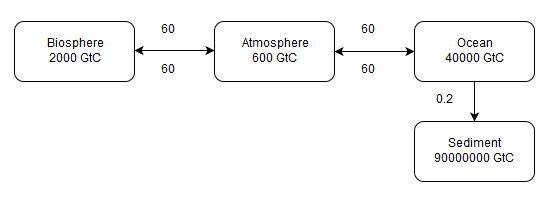
\includegraphics[scale = 0.5]{carboncycle.jpg}}
\end{center}
\end{Exercise}

\begin{Exercise}
Aftershocks can happen when an earthquake or another aftershock has occurred. Assume that the probability of aftershocks (rows) can be modelled such that it depends on the prior earthquake/aftershock only (columns), as the table shown below. Find the expected total number of earthquakes/aftershocks if there is an earthquake of magnitude 8.
\begin{center}
\begin{tabular}{|c|c|c|c|c|}
\hline
& M8 & M6-7 & M$\leq$5 & Stops\\
\hline
M8 & 0.1 & 0 & 0 & 0\\
\hline
M6-7 & 0.8 & 0.66 & 0 & 0\\
\hline
M$\leq$5 & 0.1 & 0.32 & 0.92 & 0\\
\hline
Stops & 0 & 0.02 & 0.08 & 1\\
\hline
\end{tabular}
\end{center}
Note: The numbers are made up and the real-world situation is much more complicated. Markov Chain can definitely be a tool for Seismology, but the usage will be more involved.
\end{Exercise}

\begin{Exercise}
Daniel is drunk at a bar. He wants to go to the train station so that he can go home. However, since he is drunk, he loses his sense of direction, and will move randomly along the green edge (shown in the map below) once at a time. Assume that at any starred location, the chances of moving to all other neighbouring locations are equal. Nevertheless, once he arrives at the train station, he will stop wandering and take the train. How many moves does it take on average for Daniel to reach the train station?
\begin{center}
(Placeholder for Diagram)
\end{center}
\end{Exercise}

\begin{Exercise}
Attempt \href{https://projecteuler.net/problem=84}{Project Euler Problem 84}, preferably with programming.
\end{Exercise}
\chapter{Matrix Factorization Methods}

In this chapter, we are going to discuss some matrix factorization methods. We have introduced one of them (QR Decomposition) in \autoref{chap:6}. In the past, matrix factorization is not a hot topic in Earth Science. However, as Machine Learning gains popularity in different Scientific fields, many Earth Science research starts to involve matrix factorization, which has been a main instrument in Machine Learning. Apart from this, a less visible usage of matrix factorization is embedded in the implementation of linear algebra package in programming languages (e.g. LAPACK, for Fortran). Those matrix factorization enables a much faster and stable computation of linear algebra problems, such as finding inverses or solving linear systems. Other potential applications include image processing, data compression, and more.

\section{Square Matrix Factorization}
\subsection{Cholesky Factorization}

\textit{Cholesky Decomposition} is for a special class of matrices which are symmetric and positive-definite. We have talked about how a matrix is positive-definite in section \ref{Conic}. For a symmetric and positive-definite matrix $A$, Cholesky Decomposition factorizes it into $U^TU$, where $U$ is an upper triangular matrix, $U^T$ is hence a lower triangular matrix. (Upper/lower triangular implies non-zero entries only present along or above/below the main diagonal) An example would be
\begin{align*}
A = 
\begin{bmatrix}
1 & 0 & 1 \\
0 & 1 & 1 \\
1 & 1 & 6
\end{bmatrix}
&=
\begin{bmatrix}
1 & 0 & 0 \\
0 & 1 & 0 \\
1 & 1 & 2
\end{bmatrix}
\begin{bmatrix}
1 & 0 & 1 \\
0 & 1 & 1 \\
0 & 0 & 2
\end{bmatrix} \\
&= 
\begin{bmatrix}
1 & 0 & 1 \\
0 & 1 & 1 \\
0 & 0 & 2
\end{bmatrix}^T
\begin{bmatrix}
1 & 0 & 1 \\
0 & 1 & 1 \\
0 & 0 & 2
\end{bmatrix} \\
&= U^TU 
\end{align*}

We can compute Cholesky Decomposition step by step, first rewriting the $n \times n$ matrix $A$ into the proposed factorized form of
\begin{align*}
A = U^T U = 
\begin{bmatrix}
u_{11} & \vec{r_1}^T \\
\vec{0} & U_b 
\end{bmatrix}^T
\begin{bmatrix}
u_{11} & \vec{r_1}^T \\
\vec{0} & U_b 
\end{bmatrix} = 
\begin{bmatrix}
u_{11} & \vec{0}^T \\
\vec{r_1} & U_b^T
\end{bmatrix}
\begin{bmatrix}
u_{11} & \vec{r_1}^T \\
\vec{0} & U_b 
\end{bmatrix}
\end{align*}
where $u_{11}$ is the first diagonal element of $U$, $\vec{r_1}$ is a column vector of length $n-1$ and $U_b$ is a block matrix with size $(n-1, n-1)$. The matrix dot product at R.H.S. gives
\begin{align*}
A = 
\begin{bmatrix}
\alpha_{11} & \vec{a_1}^T \\
\vec{a_1} & A_b 
\end{bmatrix}
=
\begin{bmatrix}
u_{11}^2 & u_{11}\vec{r_1}^T \\
u_{11}\vec{r_1} & \vec{r_1}\vec{r_1}^T + U_b^T U_b
\end{bmatrix}
= U^TU
\end{align*}
where $\alpha_{11}$ is the first diagonal element of $A$, $\vec{a_1}$ and $A_b$ is also a column vector just like $\vec{r_1}$ and $U_b$. The dot product involving block matrices is carried out just like usual matrix dot product. Comparing the both sides, we have
\begin{align*}
\alpha_{11} &= u_{11}^2 \\
\vec{a_1} &= u_{11}\vec{r_1} \\
A_b &= \vec{r_1}\vec{r_1}^T + U_b^T U_b
\end{align*}
\begin{align*}
u_{11} &= \sqrt{\alpha_{11}} \\
\vec{r_1} &= \frac{\vec{a_1}}{\sqrt{\alpha_{11}}} \\
U_b^T U_b &= A_b - \vec{r_1}\vec{r_1}^T
\end{align*}
By the relations above, we determine the first row and column of $U$. Subsequently, the remaining block $U_b$ is constructed by applying the same procedure on $A_2 = U_b^T U_b$ which has been obtained from the last relation, and then keep repeating the method to reduce the resulted block matrix on until the last entry is processed.
\begin{defn}
The Cholesky Factorization $U^TU$ of a symmetric, positive-definite matrix $A$, is constructed by the recursive relations
\begin{align*}
u_{mm} &= \sqrt{\alpha_{mm}} \\
\vec{r_m} &= \frac{\vec{a_m}}{\sqrt{\alpha_{mm}}} \\
U_b^T U_b &= A_b - \vec{r_m}\vec{r_m}^T
\end{align*}
where the subscript $m$ implies the $m$-th step. The formula are applied iteratively on $A_m = U_b^T U_b$ acquired at every step.
\end{defn}

\begin{exmp}
Perform Cholesky Factorization on the symmetric, positive-definite matrox
\begin{align*}
A &=
\begin{bmatrix}
4 & 2 & 0 \\
2 & 2 & 2 \\
0 & 2 & 5 
\end{bmatrix}
\end{align*}
The first step results in
\begin{align*}
u_{11} &= \sqrt{4} = \textcolor{red}{2} \\
\vec{r_1} &= \frac{1}{\sqrt{4}}
\begin{bmatrix}
2 \\
0
\end{bmatrix}
= 
\begin{bmatrix}
\textcolor{blue}{1} \\
\textcolor{blue}{0}
\end{bmatrix} \\
A_2 = U_b^T U_b &= 
\begin{bmatrix}
2 & 2 \\
2 & 5
\end{bmatrix}
-
\begin{bmatrix}
1 \\
0
\end{bmatrix}
\begin{bmatrix}
1 & 0
\end{bmatrix} \\
&= \begin{bmatrix}
1 & 2 \\
2 & 5 
\end{bmatrix}
\end{align*}
So we know that
\begin{align*}
U &=
\begin{bmatrix}
\textcolor{red}{2} & \textcolor{blue}{1} & \textcolor{blue}{0} \\
0 & ? & ? \\
0 & ? & ? \\
\end{bmatrix}
\end{align*}
The next iteration $A_2$ on gives
\begin{align*}
u_{22} &= \sqrt{1} = \textcolor{red}{1} \\  
\vec{r_2} &= \frac{1}{\sqrt{1}}
\begin{bmatrix}
2
\end{bmatrix}
=
\begin{bmatrix}
\textcolor{blue}{2}
\end{bmatrix} \\
U_b^T U_b &=
5 - 
\begin{bmatrix}
2
\end{bmatrix}
\begin{bmatrix}
2
\end{bmatrix} \\
&= 
\begin{bmatrix}
1
\end{bmatrix}
\end{align*}
We still need to deal with the $1 \times 1$ matrix that is left. At the third step, we simply take
\begin{align*}
u_{33} = \sqrt{1} = \textcolor{Green}{1}
\end{align*}
So the final expression of $U$ is given by
\begin{align*}
U = 
\begin{bmatrix}
2 & 1 & 0 \\
0 & \textcolor{red}{1} & \textcolor{blue}{2} \\
0 & 0 & \textcolor{Green}{1}
\end{bmatrix}
\end{align*}
Short Exercise: Check if $A = U^T U$.
\end{exmp}

\subsection{LU/LDU Factorization}

\textit{LU Factorization} is similar to Cholesky Factorization. It decomposes any matrix into one upper and one lower triangular matrix, but the original matrix needs not to be symmetric or positive-definite. The key to LU factorization is the method of Gaussian Elimination discussed in sections \ref{Echelon} and \ref{subsection:invGauss}. By Gaussian Elimination we can always reduce a given matrix to an upper triangular matrix (row echelon form), through a sequence of elementary row operations, or equivalently taking the dot product with a sequence of elementary matrices to the left. \\
\\
Denote such operations with $E_1', E_2', \cdots, E_n'$, in the spirit similar to theorem \ref{GaussElimPrinciple}, we have $E_n'\cdots E_2'E_1'A = U$, where $U$ is an upper triangular matrix produced from the forward phase of Gaussian Elimination. Rearrangement gives
\begin{align*}
A = (E_1'^{-1}E_2'^{-1}\cdots E_n'^{-1})U    
\end{align*}
If all $E_i'$ involves no row interchanges, then they would be all lower triangular matrices as required by the forward stage of Gaussian Elimination (if there is row interchange, then $E_i'$ will not be a lower triangular matrix.). As a result, $(E_1'^{-1}E_2'^{-1}\cdots E_n'^{-1})$ will be a lower triangular matrix $L$, and the LU Factorization $A = LU$ is constructed.
\begin{thm}
LU Factorization of a matrix $A$ is possible if it can be reduced to a row echelon form $U$, which will be an upper triangular matrix, by forward Gaussian Elimination. The steps and elementary matrices used to produce $U$ can be grouped together, and inverted to give a lower triangular matrix $L$. The LU Factorization will then be $A = LU$.
\end{thm}

\begin{exmp}
Compute a LU Factorization for
\begin{align*}
A = 
\begin{bmatrix}
2 & 0 & 0 \\
0 & 1 & 1 \\
2 & 0 & 4
\end{bmatrix}
\end{align*}
By Gaussian Elimination, we have
\begin{align*}
\begin{bmatrix}
2 & 0 & 0 \\
0 & 1 & 1 \\
2 & 0 & 4
\end{bmatrix}
&\rightarrow 
\begin{bmatrix}
1 & 0 & 0 \\
0 & 1 & 1 \\
2 & 0 & 4 
\end{bmatrix}
& E_1' =
\begin{bmatrix}
\frac{1}{2} & 0 & 0 \\
0 & 1 & 0 \\
0 & 0 & 1 \\
\end{bmatrix}
\\
&\rightarrow 
\begin{bmatrix}
1 & 0 & 0 \\
0 & 1 & 1 \\
0 & 0 & 4 
\end{bmatrix}
&
E_2' =
\begin{bmatrix}
1 & 0 & 0 \\
0 & 1 & 0 \\
-2 & 0 & 1 
\end{bmatrix}
\\
&\rightarrow 
\begin{bmatrix}
1 & 0 & 0 \\
0 & 1 & 1 \\
0 & 0 & 1
\end{bmatrix}
&
E_3' = 
\begin{bmatrix}
1 & 0 & 0 \\
0 & 1 & 0 \\
0 & 0 & \frac{1}{4}
\end{bmatrix}
\end{align*}
Therefore, we can take
\begin{align*}
U &= 
\begin{bmatrix}
1 & 0 & 0 \\
0 & 1 & 1 \\
0 & 0 & 1 
\end{bmatrix}
\\
L &= E_3'^{-1}E_2'^{-1}E_1'^{-1} \\
&=
\begin{bmatrix}
\frac{1}{2} & 0 & 0 \\
0 & 1 & 0 \\
0 & 0 & 1 
\end{bmatrix}^{-1}
\begin{bmatrix}
1 & 0 & 0 \\
0 & 1 & 0 \\
-2 & 0 & 1 
\end{bmatrix}^{-1}
\begin{bmatrix}
1 & 0 & 0 \\
0 & 1 & 0 \\
0 & 0 & \frac{1}{4} 
\end{bmatrix}
^{-1} \\
&= \begin{bmatrix}
2 & 0 & 0 \\
0 & 1 & 0 \\
0 & 0 & 1 
\end{bmatrix}
\begin{bmatrix}
1 & 0 & 0 \\
0 & 1 & 0 \\
2 & 0 & 1 
\end{bmatrix}
\begin{bmatrix}
1 & 0 & 0 \\
0 & 1 & 0 \\
0 & 0 & 4 
\end{bmatrix}
\end{align*}
This sequence amounts to a series of elementary row operations. Doing them starting from the right to the left, it is easy to arrive at
\begin{align*}
L &=
\begin{bmatrix}
2 & 0 & 0 \\
0 & 1 & 0 \\
2 & 0 & 4
\end{bmatrix}
\end{align*}
\end{exmp}

Note that LU Factorization is not unique. However, one can derive \textit{LDU Factorization} that is unique given it has one, where $D$ is a diagonal matrix, while $L$ and $U$ have all the diagonal entries being one. Using the above example, we observe that
\begin{align*}
L &=
\begin{bmatrix}
2 & 0 & 0 \\
0 & 1 & 0 \\
2 & 0 & 4
\end{bmatrix} = 
\begin{bmatrix}
1 & 0 & 0 \\
0 & 1 & 0 \\
1 & 0 & 1
\end{bmatrix}
\begin{bmatrix}
2 & 0 & 0 \\
0 & 1 & 0 \\
0 & 0 & 4
\end{bmatrix}
\end{align*}
where we factor out a diagonal matrix from $L$ to force all the entries along the main diagonal to be $1$. So the corresponding LDU Factorization is
\begin{align*}
A =
\begin{bmatrix}
1 & 0 & 0 \\
0 & 1 & 0 \\
1 & 0 & 1
\end{bmatrix}
\begin{bmatrix}
2 & 0 & 0 \\
0 & 1 & 0 \\
0 & 0 & 4
\end{bmatrix}
\begin{bmatrix}
1 & 0 & 0 \\
0 & 1 & 1 \\
0 & 0 & 1 
\end{bmatrix}
\end{align*}

There is another variant of LU Factorization which is called \textit{PLU Factorization}, applicable to any matrix $A$. The idea is to first interchange the rows in $A$ so that LU Factorization becomes possible. After obtaining the LU Factorization, we collect all the elementary row matrices involved in the initial row interchanges as a matrix $P$ to be added at the left.

\subsection{Solving Linear Systems with LU Decomposition}
As mentioned in the start of the chapter, matrix factorization helps a lot when it comes to electronic calculation. For instance, $LU$ factorization is widely applied in solving linear systems in computer, preferred over direct Gaussian Elimination or using inverse, due to the reasons we are going to discuss later.\\
\\
Basically, it involves a two step procedure. For a linear system $A\vec{x} = \vec{h}$, if we have the LU Decomposition, then it can be rewritten as $LU\vec{x} = \vec{h}$. It then becomes a two step process to solve the system, where we let $U\vec{x} = \vec{y}$, and solve $L\vec{y} = \vec{h}$ first, and then come back to solve $U\vec{x} = \vec{y}$. Due to the nature of $L$ and $U$, we can do the forward and backward substitution to solve the two systems with relative ease.

\begin{exmp}
Given a linear system $A\vec{x} = \vec{h}$, where
\begin{align*}
A &= 
\begin{bmatrix}
1 & 1 & 0 \\
0 & 2 & 2 \\
1 & 2 & 4 
\end{bmatrix}
& \vec{h} = 
\begin{bmatrix}
3 \\
2 \\
4
\end{bmatrix}
\end{align*}
and we are given the LU factorization of A as
\begin{align*}
A &= LU = 
\begin{bmatrix}
1 & 0 & 0 \\
0 & 2 & 0 \\
1 & 1 & 3 
\end{bmatrix}
\begin{bmatrix}
1 & 1 & 0 \\
0 & 1 & 1 \\
0 & 0 & 1 
\end{bmatrix}
\end{align*}
We can solve the equivalent problem $LU\vec{x} = \vec{h}$, where $U\vec{x} = \vec{y}$ and thus $L\vec{y} = \vec{h}$. The latter one leads to
\begin{align*}
\begin{bmatrix}
1 & 0 & 0 \\
0 & 2 & 0 \\
1 & 1 & 3 
\end{bmatrix}
\begin{bmatrix}
y_1 \\
y_2 \\
y_3
\end{bmatrix}
&=
\begin{bmatrix}
3 \\
2 \\
4
\end{bmatrix} \\
\vec{y} = 
\begin{bmatrix}
y_1 \\
y_2 \\
y_3
\end{bmatrix}
&=
\begin{bmatrix}
3 \\
1 \\
0
\end{bmatrix}
\end{align*}
We leave the last step of solving $U\vec{x} = \vec{y}$ to the readers, the solution of which is $\vec{x} = (2,1,0)^T$.
\end{exmp}

\paragraph{Remark} To solve a family of linear systems $A\vec{x} = \vec{h_i}$, where $\vec{h_i}$ are many different column vectors, can be very time-consuming if we use Gaussian Elimination every time. LU Decomposition extracts and encapsulates the information from Gaussian Elimination, and saves the effort needed to compute Gaussian Elimination for different $\vec{h_i}$ every time. While it is also possible to achieve similar effects by utilizing the inverse $A^{-1}$, calculating the inverse for large-scale systems can be unstable and expensive.

\section{Non-Square Matrix Factorization}

\subsection{Singular Value Decomposition}

LU Factorization can also be applied on a non-square matrix. However, there is another factorization method called \textit{Singular Value Decomposition} that is very useful in data compression. This method is not simple, and the readers may need some time to digest the instructions below. First, let's define what are singular values.
\begin{defn}
For a $m \times n$ matrix $A$, its singular values $\sigma_i$ are the square roots of the eigenvalues $\lambda_i$ of $A^TA$ (an $n \times n$ symmetric matrix, guaranteed to have $n$ eigenvalue-eigenvector pairs by theorem \ref{symdiag}). So
\begin{align*}
\sigma_i = \sqrt{\lambda_i}
\end{align*}
for $i = 1, 2, \cdots, n$.
\end{defn}
Attentive readers may notice a potential pitfall if $\lambda_i$ is negative. However, it cannot be the case. Consider the norm/length of the vector $A\hat{v_i}$ where $\hat{v_i}$ is the $i$-th unit eigenvector of $A^TA$. Then
\begin{align*}
\norm{A\hat{v_i}}^2 &= A\hat{v_i} \cdot A\hat{v_i}\\
&= \hat{v_i} \cdot (A^TA\hat{v_i}) \\
&= \hat{v_i} \cdot (\lambda_i\hat{v_i}) \\
&= \lambda_i (\hat{v_i} \cdot \hat{v_i}) = \lambda_i \norm{\hat{v_i}}^2 = \lambda_i
\end{align*}
where properties \ref{dotproper} and the definition \ref{eigen} of eigenvector are used. Since $\norm{A\vec{v_i}}^2$ must be non-negative, $\lambda_i$ will be non-negative as well. For example, the matrix
\begin{align*}
A &= 
\begin{bmatrix}
1 & 0 & 1\\
2 & 1 & 0
\end{bmatrix}
\end{align*}
leads to
\begin{align*}
A^TA &= 
\begin{bmatrix}
1 & 2\\
0 & 1 \\
1 & 0
\end{bmatrix} 
\begin{bmatrix}
1 & 0 & 1\\
2 & 1 & 0
\end{bmatrix} \\
&=
\begin{bmatrix}
5 & 2 & 1 \\
2 & 1 & 0 \\
1 & 0 & 1
\end{bmatrix}
\end{align*}
as a symmetric matrix that has eigenvalues of $\lambda = 6, 1, 0$, and hence $A$ has a sequence of singular values of $\sigma = \sqrt{6}, 1, 0$. The readers are invited to confirm the computation. We also note a key observation, that we are not going to prove. (It requires some fundamental concepts that we have chosen not to be included in the book)
\begin{thm}
For a $m \times n$ matrix $A$, where $m < n$, so that $A$ has more columns than rows, then there must be at least $n-m$ zero eigenvalues for $A^TA$, and hence the same number of zero singular values for $A$.
\end{thm}
If $m > n$, it is obvious that there are only at most $n$ eigenvalues for $A^TA$. Collectively, it implies that for a $m \times n$ matrix $A$, it will have at most $\min(m,n)$ (the smaller of $m$ and $n$) non-zero singular values. This is consistent with the example we have seen above. Now we are prepared to see how Singular Value Decomposition is done.
\begin{defn}
The Singular Value Decomposition for a $m \times n$ matrix $A$ is
\begin{align*}
A = U\Sigma V^T
\end{align*}
where $U$, $\Sigma$, $V$ is a $m \times m$, $m \times n$ and $n \times n$ matrix. $V$ is constructed by
\begin{align*}
V = 
\begin{bmatrix}
\hat{v_1} | \hat{v_2} | \cdots | \hat{v_n}
\end{bmatrix}
\end{align*}
where the unit column vectors $\hat{v_1}, \hat{v_2}, \cdots, \hat{v_n}$ are the orthonormal eigenvectors of the symmetric matrix $A^TA$ (refers to the notes for theorem \ref{symdiag}), ordered by decreasing eigenvalues. $\Sigma$ consists of the non-zero singular values $\sigma_j$ (also in decreasing order) of the corresponding column vectors $\hat{v_j}$ in $V$ along the main diagonal, and has a value of zero elsewhere. $U$ is made up of the unit column vectors (that are also orthogonal to each other) that satisfies
\begin{align*}
\hat{u_j} = \frac{1}{\sigma_j} A\hat{v_j}
\end{align*}
for all $j$ that represents a non-zero singular value $\sigma_j \neq 0$. In the case where there are not enough column vectors to construct $U$ by the relation above, use Gram-Schmidt Orthogonalization (or other feasible methods) to create orthonormal vectors that extend the basis of $\hat{u_j}$ up to $j = m$.
\end{defn}

\begin{exmp}
Again, for the $2 \times 3$ matrix
\begin{align*}
A &= 
\begin{bmatrix}
1 & 0 & 1\\
2 & 1 & 0
\end{bmatrix}
\end{align*}    
We have show that the eigenvalues of $A^TA$ are $\lambda = 6,1,0$, and the singular values of $A$ are $\sigma = \sqrt{6}, 1, 0$. The corresponding unit eigenvectors for $A^TA$ are $(\frac{\sqrt{5}}{\sqrt{6}}, \frac{\sqrt{2}}{\sqrt{15}}, \frac{1}{\sqrt{30}})^T$, $(0, -\frac{1}{\sqrt{5}}, \frac{2}{\sqrt{5}})^T$, and $(-\frac{1}{\sqrt{6}}, \frac{2}{\sqrt{6}}, \frac{1}{\sqrt{6}})^T$. So we have
\begin{align*}
&V =
\begin{bmatrix}
\frac{\sqrt{5}}{\sqrt{6}} & 0 & -\frac{1}{\sqrt{6}}\\
\frac{\sqrt{2}}{\sqrt{15}} & -\frac{1}{\sqrt{5}} & \frac{2}{\sqrt{6}}\\
\frac{1}{\sqrt{30}} & \frac{2}{\sqrt{5}} & \frac{1}{\sqrt{6}}
\end{bmatrix}
&\Sigma =
\begin{bmatrix}
\sqrt{6} & 0 & 0 \\
0 & 1 & 0
\end{bmatrix}
\end{align*}
The two column vectors for $U$ are found by
\begin{align*}
\hat{u_1} &= \frac{1}{\sigma_1} A\hat{v_1} \\
&= \frac{1}{\sqrt{6}}
\begin{bmatrix}
1 & 0 & 1\\
2 & 1 & 0
\end{bmatrix}
\begin{bmatrix}
\frac{\sqrt{5}}{\sqrt{6}} \\
\frac{\sqrt{2}}{\sqrt{15}} \\
\frac{1}{\sqrt{30}}
\end{bmatrix} \\
&=
\begin{bmatrix}
\frac{1}{\sqrt{5}} \\
\frac{2}{\sqrt{5}}
\end{bmatrix}
\end{align*}
and
\begin{align*}
\hat{u_2} &= \frac{1}{1}
\begin{bmatrix}
1 & 0 & 1\\
2 & 1 & 0
\end{bmatrix}
\begin{bmatrix}
0 \\
-\frac{1}{\sqrt{5}} \\
\frac{2}{\sqrt{5}}
\end{bmatrix} \\
&= 
\begin{bmatrix}
\frac{2}{\sqrt{5}} \\
-\frac{1}{\sqrt{5}}
\end{bmatrix}
\end{align*}
\end{exmp}
Therefore, we conclude that
\begin{align*}
U &=
\begin{bmatrix}
\frac{1}{\sqrt{5}} & \frac{2}{\sqrt{5}} \\
\frac{2}{\sqrt{5}} & -\frac{1}{\sqrt{5}}
\end{bmatrix} \\
A &= U\Sigma V^T \\
&= 
\begin{bmatrix}
\frac{1}{\sqrt{5}} & \frac{2}{\sqrt{5}} \\
\frac{2}{\sqrt{5}} & -\frac{1}{\sqrt{5}}
\end{bmatrix}
\begin{bmatrix}
\sqrt{6} & 0 & 0 \\
0 & 1 & 0
\end{bmatrix}
\begin{bmatrix}
\frac{\sqrt{5}}{\sqrt{6}} & \frac{\sqrt{2}}{\sqrt{15}} & \frac{1}{\sqrt{30}} \\
0 & -\frac{1}{\sqrt{5}} & \frac{2}{\sqrt{5}} \\
-\frac{1}{\sqrt{6}} & \frac{2}{\sqrt{6}} & \frac{1}{\sqrt{6}}
\end{bmatrix}
\end{align*}

\begin{exmp}
Carry out Singular Value Decomposition for the $3 \times 2$ matrix
\begin{align*}
A =
\begin{bmatrix}
1 & 1 \\
0 & 1 \\
1 & 0
\end{bmatrix}
\end{align*}
We leave to the readers to check that the orthonormal eigenvectors of 
\begin{align*}
A^TA = 
\begin{bmatrix}
2 & 1 \\
1 & 2
\end{bmatrix}
\end{align*}
are 
\begin{align*}
& \hat{v_1} =
\begin{bmatrix}
\frac{1}{\sqrt{2}} \\
\frac{1}{\sqrt{2}}
\end{bmatrix}
& \hat{v_2} =
\begin{bmatrix}
-\frac{1}{\sqrt{2}} \\
\frac{1}{\sqrt{2}}
\end{bmatrix}
\end{align*}
for $\lambda_1 = 3$, $\lambda_2 = 1$, so $\sigma_1 = \sqrt{3}$, $\sigma_2 = 1$, and
\begin{align*}
\Sigma =
\begin{bmatrix}
\sqrt{3} & 0 \\
0 & 1 \\
0 & 0
\end{bmatrix}   
\end{align*}
$\hat{u_1}$, $\hat{u_2}$ are then given by
\begin{align*}
\hat{u_1} &= \frac{1}{\sqrt{3}}A
\begin{bmatrix}
\frac{1}{\sqrt{2}} \\
\frac{1}{\sqrt{2}}
\end{bmatrix}
=
\begin{bmatrix}
\frac{2}{\sqrt{6}} \\
\frac{1}{\sqrt{6}} \\
\frac{1}{\sqrt{6}} 
\end{bmatrix} \\
\hat{u_1} &= \frac{1}{1}A
\begin{bmatrix}
-\frac{1}{\sqrt{2}} \\
\frac{1}{\sqrt{2}}
\end{bmatrix}
=
\begin{bmatrix}
0 \\
\frac{1}{\sqrt{2}} \\
-\frac{1}{\sqrt{2}} 
\end{bmatrix}
\end{align*}
We need another unit vector $\hat{u_3}$ that is orthogonal to both $\hat{u_1}$, $\hat{u_2}$. A quick way for the special case of three-dimensional vector is to find the cross product $\hat{u_1} \times \hat{u_2}$, that is
\begin{align*}
\hat{u_3} &= \hat{u_1} \times \hat{u_2} \\
&=
\begin{vmatrix}
\hat{i} & \hat{j} & \hat{k} \\
\frac{2}{\sqrt{6}} & \frac{1}{\sqrt{6}} & \frac{1}{\sqrt{6}}  \\
0 & \frac{1}{\sqrt{2}} & -\frac{1}{\sqrt{2}}
\end{vmatrix}
= -\frac{1}{\sqrt{3}} \hat{i} + \frac{1}{\sqrt{3}} \hat{j} + \frac{1}{\sqrt{3}} \hat{k}
\end{align*}
\end{exmp}
As a result,
\begin{align*}
U &=
\begin{bmatrix}
\frac{2}{\sqrt{6}} & 0 & -\frac{1}{\sqrt{3}} \\
\frac{1}{\sqrt{6}} & \frac{1}{\sqrt{2}} & \frac{1}{\sqrt{3}}\\
\frac{1}{\sqrt{6}} & -\frac{1}{\sqrt{2}} & \frac{1}{\sqrt{3}}
\end{bmatrix} \\
A &= U\Sigma V^T \\
&= 
\begin{bmatrix}
\frac{2}{\sqrt{6}} & 0 & -\frac{1}{\sqrt{3}} \\
\frac{1}{\sqrt{6}} & \frac{1}{\sqrt{2}} & \frac{1}{\sqrt{3}}\\
\frac{1}{\sqrt{6}} & -\frac{1}{\sqrt{2}} & \frac{1}{\sqrt{3}}
\end{bmatrix}
\begin{bmatrix}
\sqrt{3} & 0 \\
0 & 1 \\
0 & 0
\end{bmatrix} 
\begin{bmatrix}
\frac{1}{\sqrt{2}} & \frac{1}{\sqrt{2}}\\
-\frac{1}{\sqrt{2}} & \frac{1}{\sqrt{2}}
\end{bmatrix}
\end{align*}

\subsection{Truncated Singular Value Decomposition}
The Singular Value Decomposition of a matrix $A$
\begin{align*}
A = U\Sigma V^T = \begin{bmatrix}
\hat{u_1}|\hat{u_2}|\cdots|\hat{u_m}
\end{bmatrix}
\begin{bmatrix}
\sigma_1 & 0 & \cdots \\
0 & \sigma_2 & \\
\vdots & & \ddots
\end{bmatrix}
\left[
\begin{array}{c}
\hat{v_1}^T \\
\hline
\hat{v_2}^T \\
\hline
\cdots \\
\hline
\hat{v_n}^T
\end{array}
\right]
\end{align*}
can be reduced to the so-called \textit{Compact SVD}, by only keeping entries corresponds up to the last ($k$-th) non-zero singular value, where $U_k$ and $V_k$ only keeps the first $k$ columns, with $\Sigma_k$ being a diagonal $k \times k$ matrix that preserves the first $k$ non-zero singular values along the main diagonal. This results in
\begin{align*}
A = U\Sigma V^T = \begin{bmatrix}
\hat{u_1}|\hat{u_2}|\cdots|\hat{u_k}
\end{bmatrix}
\begin{bmatrix}
\sigma_1 & 0 & \cdots & 0 \\
0 & \sigma_2 & & \\
\vdots & & \ddots & \\
0 & & & \sigma_k
\end{bmatrix}
\left[
\begin{array}{c}
\hat{v_1}^T \\
\hline
\hat{v_2}^T \\
\hline
\cdots \\
\hline
\hat{v_k}^T
\end{array}
\right]
\end{align*}
It can also be expanded in a manner similar to Spectral Decomposition suggested at the end of section \ref{orthogonaldiagreal}, which gives
\begin{align*}

\end{align*}


\subsection{Relations to Principal Component Analysis}
\chapter{Index Notation and Introduction to Tensor}
\chapter*{Answers to Exercises}
\addcontentsline{toc}{chapter}{Answers to Exercises}
\rohead{Answer to Exercises}
\lehead{Answer to Exercises}
\shipoutAnswer
\rohead{Index}
\lehead{Index}
\printindex
%\addcontentsline{toc}{chapter}{Index}

\rohead{Bibliography}
\lehead{Bibliography}
\printbibliography[heading=bibintoc]
%\addcontentsline{toc}{chapter}{Bibliography}

\end{document}